% Options for packages loaded elsewhere
\PassOptionsToPackage{unicode}{hyperref}
\PassOptionsToPackage{hyphens}{url}
\PassOptionsToPackage{dvipsnames,svgnames,x11names}{xcolor}
%
\documentclass[
  letterpaper,
  DIV=11,
  numbers=noendperiod]{scrartcl}

\usepackage{amsmath,amssymb}
\usepackage{iftex}
\ifPDFTeX
  \usepackage[T1]{fontenc}
  \usepackage[utf8]{inputenc}
  \usepackage{textcomp} % provide euro and other symbols
\else % if luatex or xetex
  \usepackage{unicode-math}
  \defaultfontfeatures{Scale=MatchLowercase}
  \defaultfontfeatures[\rmfamily]{Ligatures=TeX,Scale=1}
\fi
\usepackage{lmodern}
\ifPDFTeX\else  
    % xetex/luatex font selection
\fi
% Use upquote if available, for straight quotes in verbatim environments
\IfFileExists{upquote.sty}{\usepackage{upquote}}{}
\IfFileExists{microtype.sty}{% use microtype if available
  \usepackage[]{microtype}
  \UseMicrotypeSet[protrusion]{basicmath} % disable protrusion for tt fonts
}{}
\makeatletter
\@ifundefined{KOMAClassName}{% if non-KOMA class
  \IfFileExists{parskip.sty}{%
    \usepackage{parskip}
  }{% else
    \setlength{\parindent}{0pt}
    \setlength{\parskip}{6pt plus 2pt minus 1pt}}
}{% if KOMA class
  \KOMAoptions{parskip=half}}
\makeatother
\usepackage{xcolor}
\setlength{\emergencystretch}{3em} % prevent overfull lines
\setcounter{secnumdepth}{5}
% Make \paragraph and \subparagraph free-standing
\makeatletter
\ifx\paragraph\undefined\else
  \let\oldparagraph\paragraph
  \renewcommand{\paragraph}{
    \@ifstar
      \xxxParagraphStar
      \xxxParagraphNoStar
  }
  \newcommand{\xxxParagraphStar}[1]{\oldparagraph*{#1}\mbox{}}
  \newcommand{\xxxParagraphNoStar}[1]{\oldparagraph{#1}\mbox{}}
\fi
\ifx\subparagraph\undefined\else
  \let\oldsubparagraph\subparagraph
  \renewcommand{\subparagraph}{
    \@ifstar
      \xxxSubParagraphStar
      \xxxSubParagraphNoStar
  }
  \newcommand{\xxxSubParagraphStar}[1]{\oldsubparagraph*{#1}\mbox{}}
  \newcommand{\xxxSubParagraphNoStar}[1]{\oldsubparagraph{#1}\mbox{}}
\fi
\makeatother

\usepackage{color}
\usepackage{fancyvrb}
\newcommand{\VerbBar}{|}
\newcommand{\VERB}{\Verb[commandchars=\\\{\}]}
\DefineVerbatimEnvironment{Highlighting}{Verbatim}{commandchars=\\\{\}}
% Add ',fontsize=\small' for more characters per line
\usepackage{framed}
\definecolor{shadecolor}{RGB}{241,243,245}
\newenvironment{Shaded}{\begin{snugshade}}{\end{snugshade}}
\newcommand{\AlertTok}[1]{\textcolor[rgb]{0.68,0.00,0.00}{#1}}
\newcommand{\AnnotationTok}[1]{\textcolor[rgb]{0.37,0.37,0.37}{#1}}
\newcommand{\AttributeTok}[1]{\textcolor[rgb]{0.40,0.45,0.13}{#1}}
\newcommand{\BaseNTok}[1]{\textcolor[rgb]{0.68,0.00,0.00}{#1}}
\newcommand{\BuiltInTok}[1]{\textcolor[rgb]{0.00,0.23,0.31}{#1}}
\newcommand{\CharTok}[1]{\textcolor[rgb]{0.13,0.47,0.30}{#1}}
\newcommand{\CommentTok}[1]{\textcolor[rgb]{0.37,0.37,0.37}{#1}}
\newcommand{\CommentVarTok}[1]{\textcolor[rgb]{0.37,0.37,0.37}{\textit{#1}}}
\newcommand{\ConstantTok}[1]{\textcolor[rgb]{0.56,0.35,0.01}{#1}}
\newcommand{\ControlFlowTok}[1]{\textcolor[rgb]{0.00,0.23,0.31}{\textbf{#1}}}
\newcommand{\DataTypeTok}[1]{\textcolor[rgb]{0.68,0.00,0.00}{#1}}
\newcommand{\DecValTok}[1]{\textcolor[rgb]{0.68,0.00,0.00}{#1}}
\newcommand{\DocumentationTok}[1]{\textcolor[rgb]{0.37,0.37,0.37}{\textit{#1}}}
\newcommand{\ErrorTok}[1]{\textcolor[rgb]{0.68,0.00,0.00}{#1}}
\newcommand{\ExtensionTok}[1]{\textcolor[rgb]{0.00,0.23,0.31}{#1}}
\newcommand{\FloatTok}[1]{\textcolor[rgb]{0.68,0.00,0.00}{#1}}
\newcommand{\FunctionTok}[1]{\textcolor[rgb]{0.28,0.35,0.67}{#1}}
\newcommand{\ImportTok}[1]{\textcolor[rgb]{0.00,0.46,0.62}{#1}}
\newcommand{\InformationTok}[1]{\textcolor[rgb]{0.37,0.37,0.37}{#1}}
\newcommand{\KeywordTok}[1]{\textcolor[rgb]{0.00,0.23,0.31}{\textbf{#1}}}
\newcommand{\NormalTok}[1]{\textcolor[rgb]{0.00,0.23,0.31}{#1}}
\newcommand{\OperatorTok}[1]{\textcolor[rgb]{0.37,0.37,0.37}{#1}}
\newcommand{\OtherTok}[1]{\textcolor[rgb]{0.00,0.23,0.31}{#1}}
\newcommand{\PreprocessorTok}[1]{\textcolor[rgb]{0.68,0.00,0.00}{#1}}
\newcommand{\RegionMarkerTok}[1]{\textcolor[rgb]{0.00,0.23,0.31}{#1}}
\newcommand{\SpecialCharTok}[1]{\textcolor[rgb]{0.37,0.37,0.37}{#1}}
\newcommand{\SpecialStringTok}[1]{\textcolor[rgb]{0.13,0.47,0.30}{#1}}
\newcommand{\StringTok}[1]{\textcolor[rgb]{0.13,0.47,0.30}{#1}}
\newcommand{\VariableTok}[1]{\textcolor[rgb]{0.07,0.07,0.07}{#1}}
\newcommand{\VerbatimStringTok}[1]{\textcolor[rgb]{0.13,0.47,0.30}{#1}}
\newcommand{\WarningTok}[1]{\textcolor[rgb]{0.37,0.37,0.37}{\textit{#1}}}

\providecommand{\tightlist}{%
  \setlength{\itemsep}{0pt}\setlength{\parskip}{0pt}}\usepackage{longtable,booktabs,array}
\usepackage{calc} % for calculating minipage widths
% Correct order of tables after \paragraph or \subparagraph
\usepackage{etoolbox}
\makeatletter
\patchcmd\longtable{\par}{\if@noskipsec\mbox{}\fi\par}{}{}
\makeatother
% Allow footnotes in longtable head/foot
\IfFileExists{footnotehyper.sty}{\usepackage{footnotehyper}}{\usepackage{footnote}}
\makesavenoteenv{longtable}
\usepackage{graphicx}
\makeatletter
\def\maxwidth{\ifdim\Gin@nat@width>\linewidth\linewidth\else\Gin@nat@width\fi}
\def\maxheight{\ifdim\Gin@nat@height>\textheight\textheight\else\Gin@nat@height\fi}
\makeatother
% Scale images if necessary, so that they will not overflow the page
% margins by default, and it is still possible to overwrite the defaults
% using explicit options in \includegraphics[width, height, ...]{}
\setkeys{Gin}{width=\maxwidth,height=\maxheight,keepaspectratio}
% Set default figure placement to htbp
\makeatletter
\def\fps@figure{htbp}
\makeatother
% definitions for citeproc citations
\NewDocumentCommand\citeproctext{}{}
\NewDocumentCommand\citeproc{mm}{%
  \begingroup\def\citeproctext{#2}\cite{#1}\endgroup}
\makeatletter
 % allow citations to break across lines
 \let\@cite@ofmt\@firstofone
 % avoid brackets around text for \cite:
 \def\@biblabel#1{}
 \def\@cite#1#2{{#1\if@tempswa , #2\fi}}
\makeatother
\newlength{\cslhangindent}
\setlength{\cslhangindent}{1.5em}
\newlength{\csllabelwidth}
\setlength{\csllabelwidth}{3em}
\newenvironment{CSLReferences}[2] % #1 hanging-indent, #2 entry-spacing
 {\begin{list}{}{%
  \setlength{\itemindent}{0pt}
  \setlength{\leftmargin}{0pt}
  \setlength{\parsep}{0pt}
  % turn on hanging indent if param 1 is 1
  \ifodd #1
   \setlength{\leftmargin}{\cslhangindent}
   \setlength{\itemindent}{-1\cslhangindent}
  \fi
  % set entry spacing
  \setlength{\itemsep}{#2\baselineskip}}}
 {\end{list}}
\usepackage{calc}
\newcommand{\CSLBlock}[1]{\hfill\break\parbox[t]{\linewidth}{\strut\ignorespaces#1\strut}}
\newcommand{\CSLLeftMargin}[1]{\parbox[t]{\csllabelwidth}{\strut#1\strut}}
\newcommand{\CSLRightInline}[1]{\parbox[t]{\linewidth - \csllabelwidth}{\strut#1\strut}}
\newcommand{\CSLIndent}[1]{\hspace{\cslhangindent}#1}

\KOMAoption{captions}{tableheading}
\makeatletter
\@ifpackageloaded{caption}{}{\usepackage{caption}}
\AtBeginDocument{%
\ifdefined\contentsname
  \renewcommand*\contentsname{Table of contents}
\else
  \newcommand\contentsname{Table of contents}
\fi
\ifdefined\listfigurename
  \renewcommand*\listfigurename{List of Figures}
\else
  \newcommand\listfigurename{List of Figures}
\fi
\ifdefined\listtablename
  \renewcommand*\listtablename{List of Tables}
\else
  \newcommand\listtablename{List of Tables}
\fi
\ifdefined\figurename
  \renewcommand*\figurename{Figure}
\else
  \newcommand\figurename{Figure}
\fi
\ifdefined\tablename
  \renewcommand*\tablename{Table}
\else
  \newcommand\tablename{Table}
\fi
}
\@ifpackageloaded{float}{}{\usepackage{float}}
\floatstyle{ruled}
\@ifundefined{c@chapter}{\newfloat{codelisting}{h}{lop}}{\newfloat{codelisting}{h}{lop}[chapter]}
\floatname{codelisting}{Listing}
\newcommand*\listoflistings{\listof{codelisting}{List of Listings}}
\makeatother
\makeatletter
\makeatother
\makeatletter
\@ifpackageloaded{caption}{}{\usepackage{caption}}
\@ifpackageloaded{subcaption}{}{\usepackage{subcaption}}
\makeatother

\ifLuaTeX
  \usepackage{selnolig}  % disable illegal ligatures
\fi
\usepackage{bookmark}

\IfFileExists{xurl.sty}{\usepackage{xurl}}{} % add URL line breaks if available
\urlstyle{same} % disable monospaced font for URLs
\hypersetup{
  pdftitle={Neuromappr},
  colorlinks=true,
  linkcolor={blue},
  filecolor={Maroon},
  citecolor={Blue},
  urlcolor={Blue},
  pdfcreator={LaTeX via pandoc}}


\title{Neuromappr}
\usepackage{etoolbox}
\makeatletter
\providecommand{\subtitle}[1]{% add subtitle to \maketitle
  \apptocmd{\@title}{\par {\large #1 \par}}{}{}
}
\makeatother
\subtitle{Brain-Computer Interface Movement Decoding Using Support
Vector Machines}
\author{Wanghley Soares Martins}
\date{2025-04-27}

\begin{document}
\maketitle

\renewcommand*\contentsname{Table of contents}
{
\hypersetup{linkcolor=}
\setcounter{tocdepth}{2}
\tableofcontents
}

\section{Introduction}\label{introduction}

\subsection{Background}\label{background}

Since the creation of machines and computers, the human interaction with
them has been evolving and sometimes quite challenging. For instance,
the first computers were operated using punch cards, which required a
lot of effort to input data. As technology advanced, we moved to
keyboards and mice, which made it easier to interact with computers.
However, these methods still require physical movement and can be
limiting for individuals with disabilities or injuries. This interaction
with computers has been a challenge investigated for researchers and
engineers for decades in the field of Human-Computer Interaction (HCI)
{[}1{]}.

The goal of HCI is to create systems that are easy to use and
understand, allowing users to interact with computers in a natural and
intuitive way. This has led to the development of various input devices,
such as touchscreens, voice recognition, and even brain-computer
interfaces (BCIs), the focus of this project.

Brain-Computer Interfaces (BCIs) are systems that enable direct
communication between the human brain and devices, bypassing the need
for physical movement and control, which can be particularly beneficial
for individuals with disabilities or injuries. Among other data, BCIs
can use electroencephalography (EEG) signals to decode brain activity
and translate it into commands for controlling devices.

BCI technology has the potential to revolutionize the way we interact
with computers and other devices, making it possible for individuals
with disabilities to regain control over their environment. Central to
the efficacy of BCIs is the accurate interpretation of
electroencephalogram (EEG) signals, particularly those associated with
motor imagery---the mental simulation of movement without actual
execution as described by Costantini et al.~(2009) {[}2{]}.

From a machine learning standpoint, the classification of EEG signals
for motor imagery tasks presents several intricate challenges:

\begin{itemize}
\tightlist
\item
  \textbf{High Dimensionality with Limited Samples}: EEG data are
  inherently high-dimensional, often involving recordings from numerous
  electrodes (e.g., 102 in this project), each capturing complex
  temporal dynamics. However, the number of labeled training samples is
  typically limited, leading to the ``curse of dimensionality,'' where
  models risk overfitting and poor generalization.
\item
  \textbf{Non-Stationarity and Noise}: EEG signals are susceptible to
  various artifacts (e.g., muscle movements, eye blinks) and exhibit
  non-stationary behavior, complicating the extraction of consistent
  features across sessions and subjects.
\item
  \textbf{Inter-Subject Variability}: There is significant variability
  in EEG signals across different individuals, which can affect the
  performance of machine learning models trained on data from a single
  subject. This variability necessitates the development of robust
  algorithms that can generalize well across different users.
\item
  \textbf{Temporal Dynamics}: EEG signals are time-dependent, and
  capturing the temporal dynamics of brain activity is crucial for
  accurate classification. This requires the use of advanced techniques
  that can model temporal relationships effectively.
\end{itemize}

Support Vector Machines (SVMs) have been extensively employed in this
domain due to their effectiveness in high-dimensional spaces and
robustness to overfitting. For instance, Costantini et al.~(2009)
{[}2{]} demonstrated the utility of SVMs in classifying EEG signals for
BCI applications, emphasizing their capacity to handle complex,
high-dimensional data.

\subsection{Objectives}\label{objectives}

In this project, we aim to implement and evaluate SVM-based classifiers
for distinguishing between left and right-hand motor imagery using EEG
data. By addressing the aforementioned challenges through appropriate
preprocessing, feature extraction, and model selection, we seek to
contribute to the development of reliable and efficient BCI systems.

\subsubsection{Spedific Objectives}\label{spedific-objectives}

\begin{enumerate}
\def\labelenumi{\arabic{enumi}.}
\tightlist
\item
  Implement a Support Vector Machine (SVM) classifier for EEG data.

  \begin{itemize}
  \tightlist
  \item
    Evaluate the performance of the SVM classifier using various kernel
    functions (linear, polynomial, and radial basis function).
  \item
    Optimize the SVM hyperparameters using grid search and
    cross-validation techniques.
  \end{itemize}
\item
  Compare the performance of the SVM classifier with Overt and Imagined
  Motor Imagery (MI) tasks.

  \begin{itemize}
  \tightlist
  \item
    Analyze the classification accuracy, precision, recall, and F1-score
    for both tasks.
  \item
    Investigate the impact of different EEG feature extraction methods
    on classification performance.
  \end{itemize}
\item
  Visualize and interpret the results of the SVM classifier, including
  feature importance and decision boundaries.

  \begin{itemize}
  \tightlist
  \item
    Provide insights into the EEG features that contribute to the
    classification performance.
  \item
    Visualize the decision boundaries of the SVM classifier in the
    feature space.
  \end{itemize}
\end{enumerate}

\subsection{Dataset overview}\label{dataset-overview}

The dataset utilized in this project comprises EEG recordings from a
Brain-Computer Interface (BCI) experiment designed to distinguish
between left and right-hand movements. The recordings are categorized
into two distinct types:

\begin{enumerate}
\def\labelenumi{\arabic{enumi}.}
\item
  \textbf{Overt Motor Imagery (OMI)}: This task involves participants
  imagining moving their left or right hand while EEG signals are
  recorded.
\item
  \textbf{Imagined Motor Imagery (IMI)}: In this task, participants are
  instructed to imagine moving their left or right hand without any
  actual movement.
\end{enumerate}

Moreover, the dataset provides the XY coordinates of the electrodes,
which are crucial for visualizing the spatial distribution of EEG
signals across the scalp. The dataset is organized into two main
folders: \texttt{data}.

The data is organized on the following files:

\begin{itemize}
\item
  \texttt{data/BCIsensor\_xy.csv}: Contains the XY coordinates of the
  electrodes.
\item
  \texttt{data/feaSubEImg\_1.csv}: Contains the EEG data for the IMI
  task for one direction (left).
\item
  \texttt{data/feaSubEImg\_2.csv}: Contains the EEG data for the IMI
  task for the other direction (right).
\item
  \texttt{data/feaSubEOvert\_1.csv}: Contains the EEG data for the OMI
  task for one direction (left).
\item
  \texttt{data/feaSubEOvert\_2.csv}: Contains the EEG data for the OMI
  task for the other direction (right).
\end{itemize}

On the electrodes' data, it is organized with each trial as a column and
each electrode on that trial as a row, as shown in
Table~\ref{tbl-electrodes}.

\begin{longtable}[]{@{}llll@{}}
\caption{Electrodes' data
organization}\label{tbl-electrodes}\tabularnewline
\toprule\noalign{}
Electrode & Trial 1 & Trial 2 & Trial 3 \\
\midrule\noalign{}
\endfirsthead
\toprule\noalign{}
Electrode & Trial 1 & Trial 2 & Trial 3 \\
\midrule\noalign{}
\endhead
\bottomrule\noalign{}
\endlastfoot
1 & Value & Value & Value \\
2 & Value & Value & Value \\
3 & Value & Value & Value \\
\end{longtable}

In terms of electrode placement, the dataset includes 102 electrodes
arranged in the configuration plotted in
Figure~\ref{fig-electrodesPositions}. The electrodes are positioned
according to the 10-20 system, a standardized method for electrode
placement in EEG studies. This system ensures consistent and
reproducible electrode locations across different subjects and studies.

\begin{figure}

\centering{

\begin{figure}
\centering
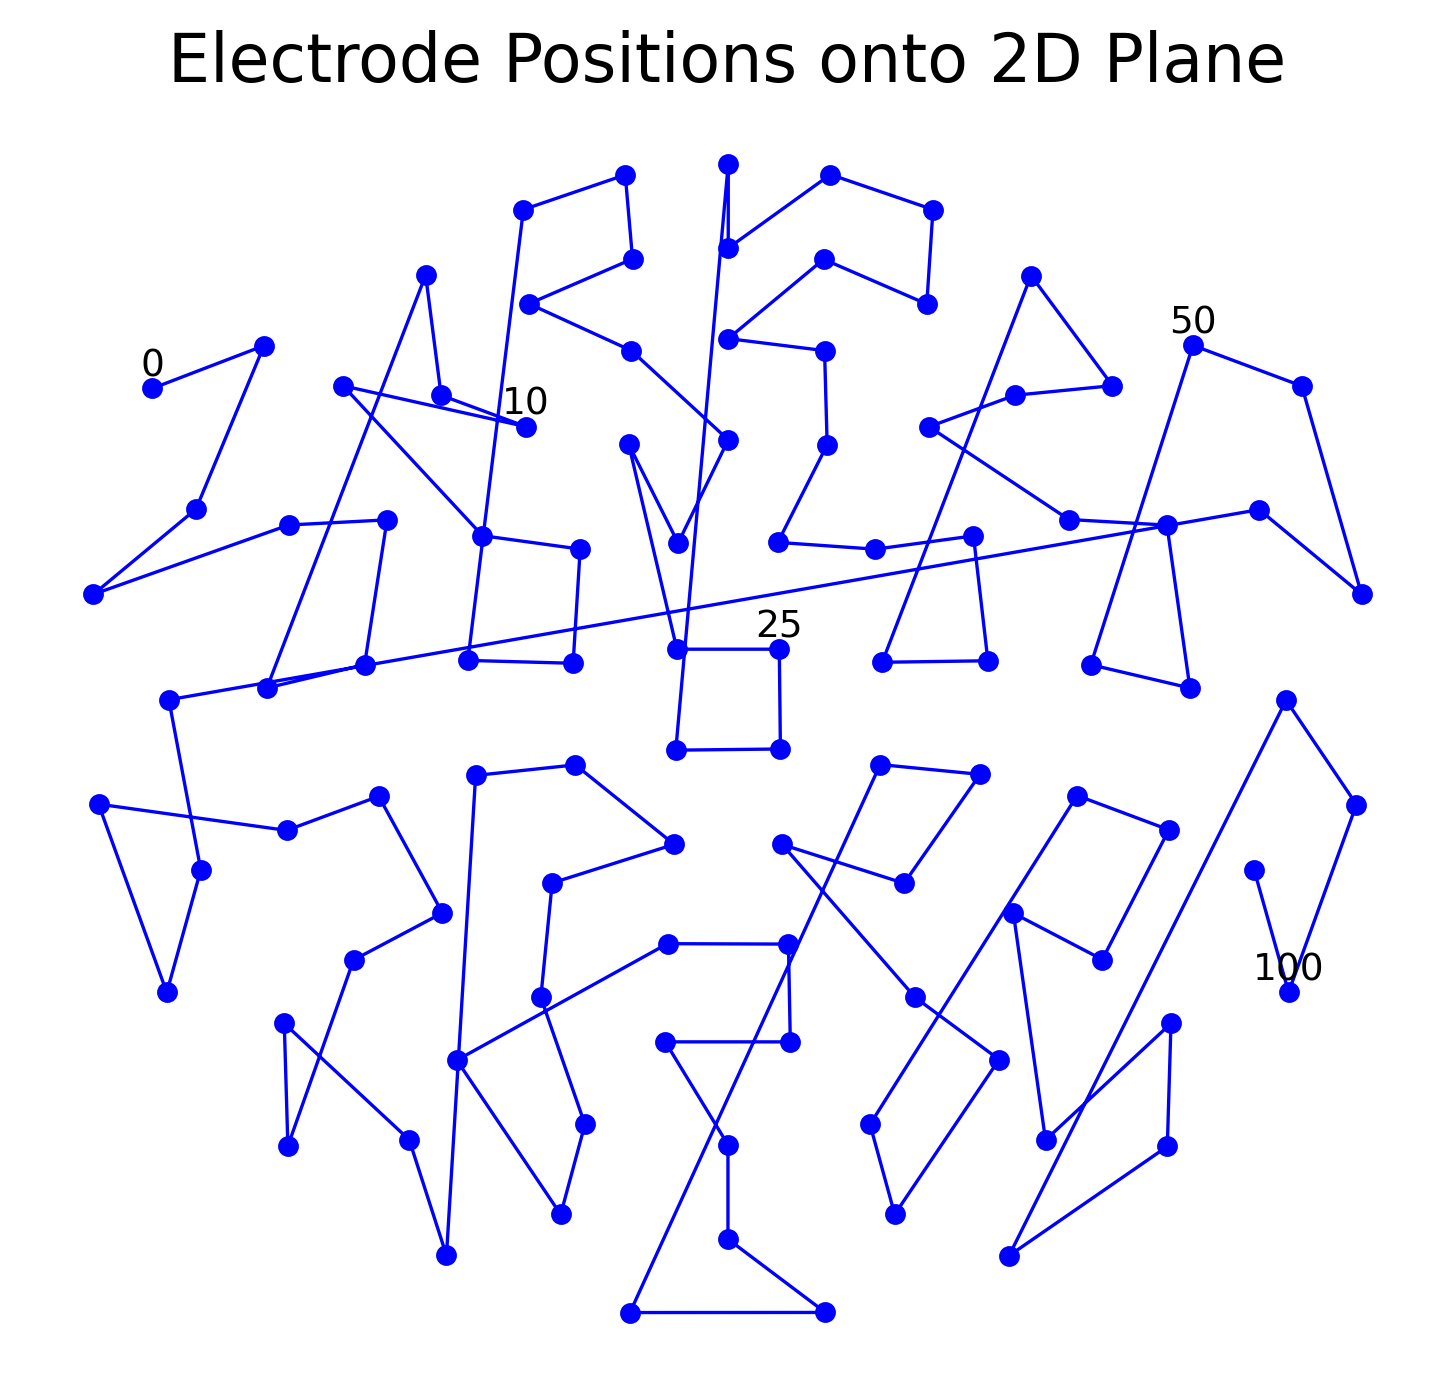
\includegraphics[width=0.7\textwidth,height=\textheight]{figures/electrode_positions.png}
\caption{Electrodes positions}\label{fig:electrodes-positions}
\end{figure}

}

\caption{\label{fig-electrodesPositions}}

\end{figure}%

\textbf{Figure~\ref{fig-electrodesPositions}} Electrode positions on the
scalp according to the 10-20 system. The numbers indicate the electrode
labels, which correspond to the columns in the dataset. Source: By the
author (2025).

A topographic view into the skull is shown in
Figure~\ref{fig-electrodesPositionsTopologic}, where the electrodes are
represented as dots on the scalp. The numbers indicate the electrode
labels, which correspond to the columns in the dataset. The topographic
representation provides a visual understanding of the spatial
distribution of EEG signals across the scalp, allowing for better
interpretation of the data.

\begin{figure}

\centering{

\begin{figure}
\centering
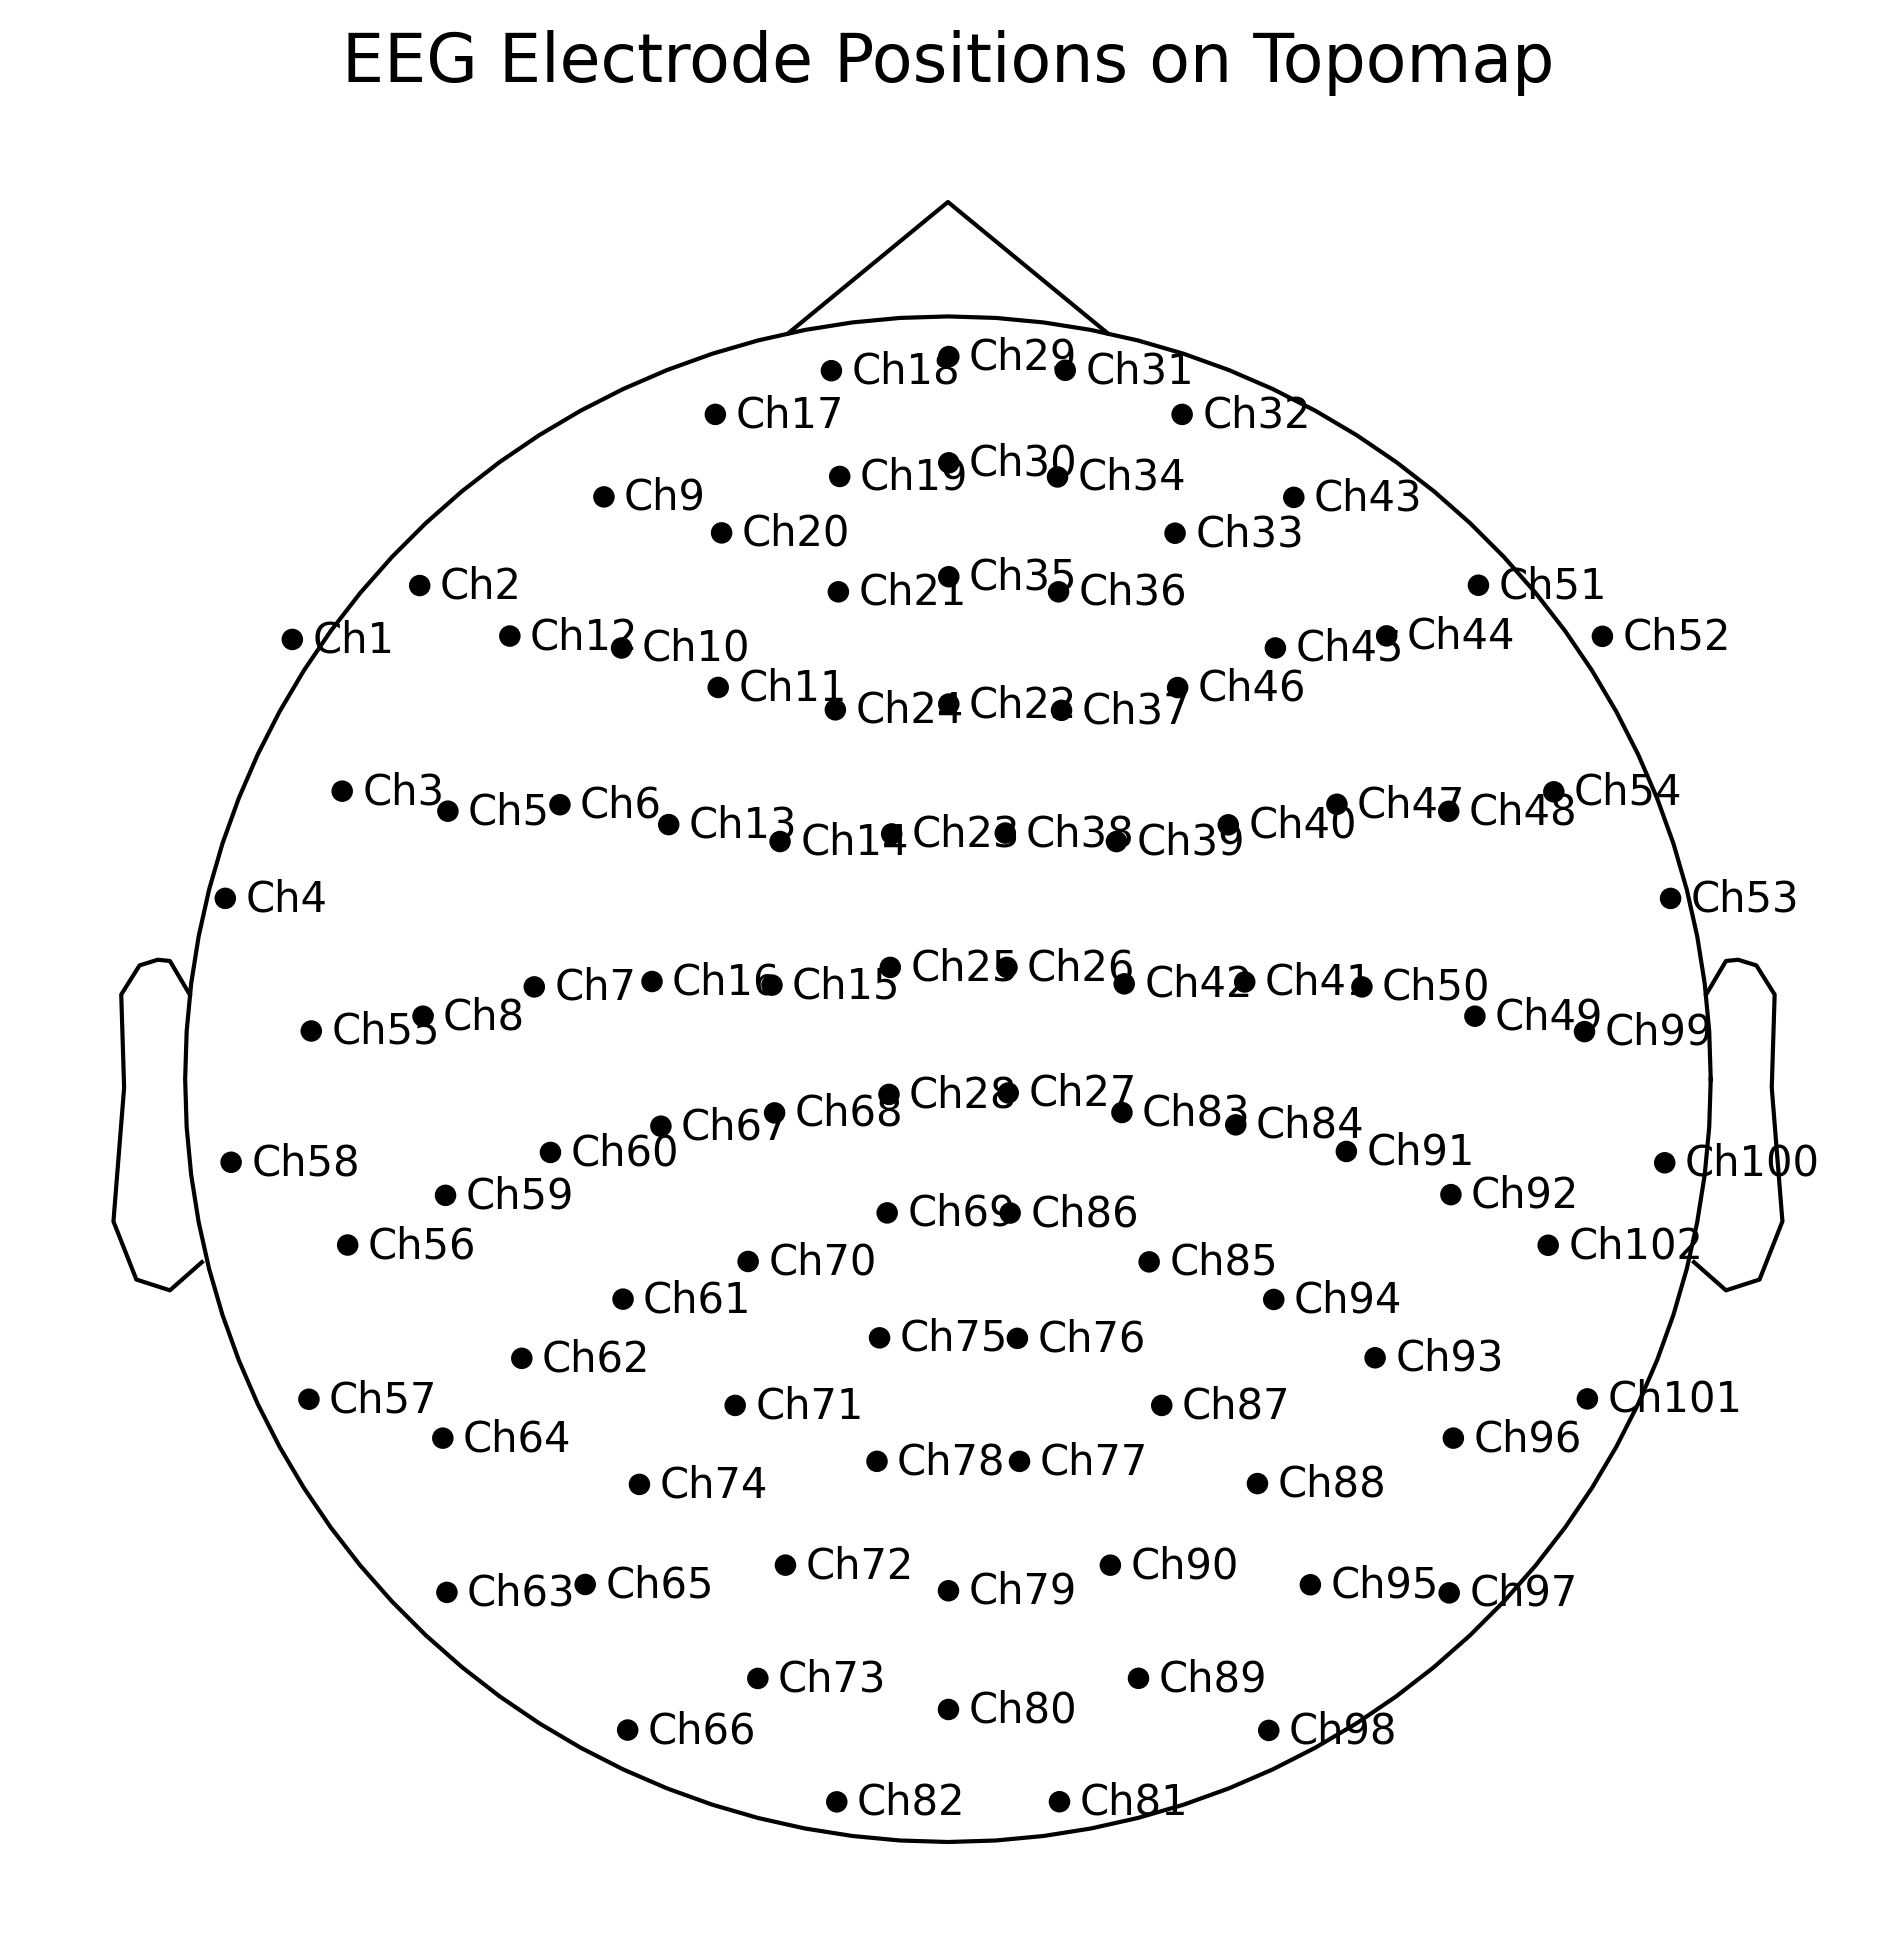
\includegraphics[width=0.7\textwidth,height=\textheight]{figures/electrode_positions_topomap.png}
\caption{Electrodes positions
topologic}\label{fig:electrodes-positions-topologic}
\end{figure}

}

\caption{\label{fig-electrodesPositionsTopologic}}

\end{figure}%

\textbf{Figure~\ref{fig-electrodesPositionsTopologic}} Topographic
representation of the electrode positions on the scalp. The numbers
indicate the electrode labels, which correspond to the columns in the
dataset. Source: By the author (2025).

\section{Methods}\label{methods}

\subsection{Project Structure}\label{project-structure}

This project follows a structured pipeline encompassing data
acquisition, signal preprocessing, classification, and
interpretation---each stage playing a critical role in the accurate
decoding of motor imagery from EEG signals. Inspired by the workflow
presented in Wu et al.~(2018){[}3{]}, this architecture promotes
clarity, reproducibility, and alignment with current practices in
EEG-based Brain-Computer Interface (BCI) research.

As shown in \textbf{Figure~\ref{fig-pipeline}}, the end-to-end system
begins with EEG signal generation through motor-related brain activity,
followed by collection via sensor-equipped EEG caps. The recorded
signals then undergo preprocessing and are classified using machine
learning algorithms---particularly Support Vector Machines (SVMs)---to
distinguish between motor imagery classes. The final output may be
translated into control commands or used for further neurophysiological
interpretation.

\begin{figure}

\centering{

\begin{figure}
\centering
\includegraphics[width=0.7\textwidth,height=\textheight]{assets/wu1-p4-wu-large.gif}
\caption{Project pipeline}\label{fig:project-pipeline}
\end{figure}

}

\caption{\label{fig-pipeline}}

\end{figure}%

\textbf{Figure~\ref{fig-pipeline}:} Conceptual workflow from EEG
activity to application.\\
Source: adapted from Wu et al.~(2018) {[}3{]}.

This representation effectively illustrates the typical stages of a BCI
system: (1) EEG generation through neural activity, (2) signal
acquisition, (3) processing and classification (often including feature
extraction and transformation into actionable information), and (4)
deployment or application, such as robotic actuation or interface
control.

The focus on this paper is on the signal processing and classification
stages, where we will implement a Support Vector Machine (SVM)
classifier to decode motor imagery tasks from EEG signals. We will not
delve into the EEG generation and acquisition stages, as they are
outside the scope of this project.

\subsection{Mathematical Formulation}\label{mathematical-formulation}

\subsubsection{Support Vector Machines: A Mathematical Framework for
High-Dimensional EEG
Classification}\label{support-vector-machines-a-mathematical-framework-for-high-dimensional-eeg-classification}

In this project, Support Vector Machines (SVMs) are utilized to classify
EEG signals corresponding to left and right-hand movement, either overt
or imagined. The application of SVMs to EEG data is particularly
well-justified: these classifiers are known to perform effectively in
high-dimensional spaces, especially when the number of observations is
small relative to the number of features---a condition that closely
matches our dataset, which consists of 204 features per trial but only
240 trials per condition.

The primary objective of an SVM is to find a hyperplane that best
separates two classes in the feature space. In the simplest case, where
data are linearly separable, a linear SVM seeks the hyperplane that
maximizes the margin between the two classes. For a given trial
\(\mathbf{x}_i \in \mathbb{R}^{204}\) with class label
\(y_i \in \{-1, +1\}\), the classifier has the form:

\[
f(\mathbf{x}) = \mathbf{w}^\top \mathbf{x} + b
\]

Here, \(\mathbf{w}\) is the weight vector orthogonal to the decision
boundary, and \(b\) is the bias term. The training process identifies
the optimal \(\mathbf{w}\) and \(b\) such that the margin---the distance
between the hyperplane and the closest points of each class---is
maximized, such as ilustrated on Figure~\ref{fig-svm} by Dai et. al
(2020) {[}4{]}. This is achieved by solving the following convex
optimization problem:

\[
\min_{\mathbf{w}, b} \frac{1}{2} \|\mathbf{w}\|^2
\quad \text{subject to} \quad
y_i (\mathbf{w}^\top \mathbf{x}_i + b) \geq 1
\]

\begin{figure}

\centering{

\includegraphics[width=0.4\textwidth,height=\textheight]{assets/814300a230-fig-1-source-large.gif}

}

\caption{\label{fig-svm}}

\end{figure}%

\textbf{Figure 2:} Support Vector Machine (SVM) illustration. The dashed
line represents the decision boundary, while the solid lines indicate
the margin. The support vectors are the data points closest to the
decision boundary {[}4{]}.

This formulation is known as the \textbf{hard-margin SVM}, suitable only
when the data is perfectly separable. In practice, particularly with EEG
data, perfect separation is unrealistic due to measurement noise,
physiological artifacts, and signal overlap between classes. Thus, we
turn to the \textbf{soft-margin SVM}, which introduces slack variables
\(\xi_i \geq 0\) that allow some misclassification, yielding a more
robust solution:

\[
\min_{\mathbf{w}, b, \boldsymbol{\xi}} \frac{1}{2} \|\mathbf{w}\|^2 + C \sum_{i=1}^{n} \xi_i
\quad \text{subject to} \quad
y_i (\mathbf{w}^\top \mathbf{x}_i + b) \geq 1 - \xi_i
\]

The parameter \(C > 0\) controls the trade-off between maximizing the
margin and minimizing classification errors. A smaller \(C\) permits
more violations (larger margin, higher bias), while a larger \(C\)
enforces stricter separation (lower bias, higher variance). This
parameter is crucial in EEG classification, particularly when comparing
performance on imagined versus overt movement data, as imagined
movements tend to be more subtle and noisy.

An important property of SVMs is that they produce not only binary class
decisions, but also \textbf{decision statistics}. For any trial
\(\mathbf{x}\), the signed output
\(f(\mathbf{x}) = \mathbf{w}^\top \mathbf{x} + b\) quantifies the
distance of the trial from the decision boundary. This value is used to
compute performance metrics such as ROC curves and can serve as a
confidence measure for the prediction. The ability to produce such a
statistic, rather than just a class label, is a key reason SVMs are
well-suited to this project.

Moreover, the learned weight vector \(\mathbf{w}\) in a linear SVM
offers meaningful insight into the relative importance of each feature.
In our case, EEG features are structured as 204 elements, corresponding
to 102 electrodes each providing two components: the x-gradient and
y-gradient of the electric field. To interpret the contribution of each
electrode, we compute the magnitude of each Ex/Ey pair:

\[
w_k = \sqrt{w_{2k-1}^2 + w_{2k}^2}, \quad k = 1, \dots, 102
\]

This produces a 102-element vector indicating the relative influence of
each electrode on the classification decision. The resulting magnitudes
are mapped onto a topographic layout of the head, allowing spatial
visualization of the most informative brain regions.

While the linear SVM provides interpretability, it may not fully capture
complex, nonlinear relationships in the EEG signals. To address this, we
also consider \textbf{kernel SVMs}, which implicitly map the data into
higher-dimensional feature spaces via kernel functions. These functions
compute inner products in the transformed space without requiring
explicit transformation, a technique known as the \textbf{kernel trick}.
The decision function becomes:

\[
f(\mathbf{x}) = \sum_{i \in \mathcal{S}} \alpha_i y_i k(\mathbf{x}_i, \mathbf{x}) + b
\]

Here, \(\mathcal{S}\) is the set of support vectors, and
\(k(\cdot, \cdot)\) is a kernel function. We explore multiple kernel
types in this project, including:

\begin{itemize}
\tightlist
\item
  \textbf{Linear:} baseline, interpretable, fast;
\item
  \textbf{Radial Basis Function (RBF):} capable of capturing smooth
  nonlinearities;
\item
  \textbf{Sigmoid:} similar to neural networks, less common in practice;
\item
  \textbf{Polynomial:} included for completeness and comparison.
\end{itemize}

In kernel SVMs, we lose direct access to the weight vector
\(\mathbf{w}\), making interpretability more challenging. To address
this, we use \textbf{permutation importance} to estimate the relative
importance of each feature for nonlinear kernels.

Implementation of SVMs in this project is performed using the
\texttt{sklearn.svm} module, which provides a user-friendly interface
for training and evaluating SVM classifiers. The \texttt{SVC} class
allows for easy specification of kernel types, hyperparameters, and
performance metrics.

\subsubsection{Permutation Importance}\label{permutation-importance}

Let
\(X = [\mathbf{x}_1, \dots, \mathbf{x}_n]^\top \in \mathbb{R}^{n \times d}\)
be the EEG data matrix and \(f\) the trained classifier. The permutation
importance of feature \(j\) is estimated as:

\begin{enumerate}
\def\labelenumi{\arabic{enumi}.}
\item
  Compute the \textbf{baseline score} (e.g., accuracy or AUC) on the
  original test data:\\
  \[
  s_{\text{baseline}} = \text{score}(f, X, y)
  \]
\item
  For each feature \(j\), create a perturbed version \(X^{(j)}\) where
  the \(j^{th}\) column is randomly shuffled across all samples.
\item
  Evaluate the performance on the perturbed data:\\
  \[
  s^{(j)} = \text{score}(f, X^{(j)}, y)
  \]
\item
  Define the \textbf{importance} of feature \(j\) as the performance
  drop: \[
  \text{Importance}_j = s_{\text{baseline}} - s^{(j)}
  \]
\end{enumerate}

This process is repeated over multiple random permutations (e.g., 10
times), and the mean drop in performance is taken as the final estimate
of the feature's importance.

\textbf{Implementation in This Project:}

In our kernel SVM experiments, we used
\texttt{sklearn.inspection.permutation\_importance} with the following
settings:

\begin{itemize}
\tightlist
\item
  \texttt{n\_repeats=10} to average out noise in the performance
  estimates,
\item
  \texttt{scoring=\textquotesingle{}accuracy\textquotesingle{}} or
  \texttt{\textquotesingle{}roc\_auc\textquotesingle{}} depending on the
  metric of interest,
\item
  \texttt{n\_jobs=-1} to parallelize computation across all available
  cores.
\end{itemize}

This method yielded a 204-dimensional vector representing the importance
of each feature (i.e., each EEG gradient channel). To visualize the
spatial contributions of the electrodes, we paired each \(\text{Ex}\)
and \(\text{Ey}\) component and computed a magnitude-based importance
score for each electrode:

\[
w_k = \sqrt{\text{Importance}_{2k-1}^2 + \text{Importance}_{2k}^2}, \quad k = 1, \dots, 102
\]

These values were mapped onto the scalp using topographic plots to
interpret which brain regions most strongly contributed to
classification, despite the underlying SVM model being nonlinear and not
directly interpretable.

\subsubsection{Extending SVMs with Kernels for Nonlinear EEG
Classification}\label{extending-svms-with-kernels-for-nonlinear-eeg-classification}

While linear Support Vector Machines (SVMs) provide a robust and
interpretable foundation for classifying EEG data, they assume that the
classes are separable by a linear boundary in the original feature
space. However, EEG signals---especially those corresponding to imagined
movements---often exhibit complex, nonlinear patterns that cannot be
adequately captured using linear decision functions. To address this, we
incorporate \textbf{kernel methods}, which allow SVMs to construct
flexible, nonlinear decision boundaries by implicitly mapping data into
higher-dimensional spaces.

In the kernelized SVM, we represent the decision function as:

\[
f(\mathbf{x}) = \sum_{i=1}^{n} \alpha_i y_i k(\mathbf{x}_i, \mathbf{x}) + b
\]

Here, - \(\mathbf{x}_i\) are the training samples, -
\(y_i \in \{-1, +1\}\) are the labels, - \(\alpha_i\) are the learned
Lagrange multipliers, - \(k(\mathbf{x}_i, \mathbf{x})\) is the kernel
function measuring similarity, - \(b\) is the bias term.

Only the training samples with \(\alpha_i > 0\) (support vectors)
contribute to the decision function. The function \(f(\mathbf{x})\)
returns a continuous \textbf{decision statistic}, and its sign
determines the predicted class.

\paragraph{Kernels Used in This
Project}\label{kernels-used-in-this-project}

We explore four kernel types, each with unique geometric and
computational properties:

\begin{enumerate}
\def\labelenumi{\arabic{enumi}.}
\item
  \textbf{Linear Kernel} (baseline): \[
  k(\mathbf{x}_i, \mathbf{x}_j) = \mathbf{x}_i^\top \mathbf{x}_j
  \] Used for direct interpretability and comparison with non-kernel
  results.
\item
  \textbf{Radial Basis Function (RBF) Kernel}: \[
  k(\mathbf{x}_i, \mathbf{x}_j) = \exp(-\gamma \|\mathbf{x}_i - \mathbf{x}_j\|^2)
  \] Introduces local flexibility, useful for capturing subtle
  nonlinearity in noisy EEG signals. The hyperparameter \(\gamma\)
  controls the influence of individual training points.
\item
  \textbf{Polynomial Kernel}: \[
  k(\mathbf{x}_i, \mathbf{x}_j) = (\gamma \mathbf{x}_i^\top \mathbf{x}_j + r)^d
  \] Enables modeling more complex global relationships between
  channels. Requires tuning of degree \(d\), scale \(\gamma\), and
  offset \(r\).
\item
  \textbf{Sigmoid Kernel}: \[
  k(\mathbf{x}_i, \mathbf{x}_j) = \tanh(\gamma \mathbf{x}_i^\top \mathbf{x}_j + r)
  \] Related to neural network activation functions, but less commonly
  used due to its sensitivity to hyperparameter settings.
\end{enumerate}

Each kernel introduces its own set of hyperparameters, which are
optimized during the \textbf{inner loop of the two-level
cross-validation} strategy used in this project.

\paragraph{Kernel Selection Strategy}\label{kernel-selection-strategy}

For each kernel, we trained a model on EEG trials using the same
cross-validation framework and computed performance metrics including
accuracy and ROC area. This allowed us to compare not only final
performance but also generalization stability across folds.

The goal was not to ``pick the best kernel'' outright, but rather to
understand the types of decision boundaries each kernel enables and how
well they adapt to the EEG signal characteristics for both overt and
imagined movement trials.

\begin{itemize}
\tightlist
\item
  \textbf{RBF kernels} generally performed better on imagined movement
  data, likely due to their ability to adapt to low signal-to-noise
  ratios.
\item
  \textbf{Linear kernels} offered clearer interpretability and often
  comparable performance on overt movement data, where class separation
  is stronger.
\item
  \textbf{Polynomial kernels} showed some promise in capturing
  intermediate complexity but were more prone to overfitting unless
  carefully regularized.
\end{itemize}

\paragraph{Interpretation of Kernel
SVMs}\label{interpretation-of-kernel-svms}

Unlike linear SVMs, kernelized models do not produce a weight vector
\(\mathbf{w}\) in the input space. As such, \textbf{direct
interpretation of feature contributions is not possible}. To bridge this
gap, we applied \textbf{permutation importance}, which measures how
shuffling each feature affects classification performance (as described
in a previous section).

To interpret these results spatially, we paired each Ex/Ey feature,
computed magnitudes, and visualized electrode-wise importance on a scalp
topomap. This enabled us to identify cortical regions that played a key
role in the model's classification decisions, even in the absence of
explicit feature weights.

\subsubsection{Regularization Parameter and Norm Penalties in
SVMs}\label{regularization-parameter-and-norm-penalties-in-svms}

In Support Vector Machines (SVMs), the \textbf{regularization parameter
\(C\)} is critical to managing the trade-off between model complexity
and classification accuracy. Particularly in the context of EEG-based
Brain-Computer Interface (BCI) classification, where high-dimensional
and noisy data are prevalent, appropriate regularization ensures robust
generalization to unseen trials.

Regularization is not just a technique for numerical stability---it
fundamentally shapes the classifier's bias-variance tradeoff and governs
what kind of solution is learned {[}5{]}. For BCI movement decoding,
where noisy, high-dimensional data are the norm, choosing the right
regularization strategy is crucial to achieving both accuracy and
interpretability.

\paragraph{\texorpdfstring{Soft-Margin SVM and the Role of
\(C\)}{Soft-Margin SVM and the Role of C}}\label{soft-margin-svm-and-the-role-of-c}

For EEG classification, we typically rely on the \textbf{soft-margin
SVM}, which tolerates some misclassification to allow for greater
generalization {[}5{]}. The \textbf{primal optimization problem} is
given by:

\[
\min_{\mathbf{w}, b, \boldsymbol{\xi}} \ \frac{1}{2} \|\mathbf{w}\|^2 + C \sum_{i=1}^{n} \xi_i
\quad \text{subject to} \quad
y_i (\mathbf{w}^\top \mathbf{x}_i + b) \geq 1 - \xi_i, \quad \xi_i \geq 0
\]

Here: - \(\|\mathbf{w}\|^2\) is the \textbf{L2 norm squared},
encouraging small weights and a large-margin hyperplane, - \(C\)
controls the penalty for slack variable \(\xi_i\), which quantifies
margin violations.

This formulation is an instance of \textbf{Ridge-like regularization}
applied to an SVM. It penalizes large weights quadratically, resulting
in smooth decision boundaries and improved stability---ideal for
high-dimensional EEG data where overfitting is a risk {[}5{]}.

\paragraph{L2 Regularization (Ridge): Smooth and
Stable}\label{l2-regularization-ridge-smooth-and-stable}

L2 regularization adds a quadratic penalty on the magnitude of the
weights:

\[
\mathcal{L}_{\text{L2}}(\mathbf{w}) = \frac{1}{2} \|\mathbf{w}\|^2 = \frac{1}{2} \sum_{j=1}^{d} w_j^2
\] {[}5{]}.

This approach: - Encourages all weights to be small but nonzero, -
Produces \textbf{dense models}, where most features contribute a little,
- Is suitable when all features (i.e., EEG channels) may carry signal
but none dominate.

In our project, this penalty was particularly useful for classifying
overt movement EEG, where clean signal and broader spatial activation
are expected.

\paragraph{L1 Regularization (Lasso): Sparsity and
Interpretability}\label{l1-regularization-lasso-sparsity-and-interpretability}

An alternative to L2 is \textbf{L1 regularization}, which penalizes the
\textbf{absolute value} of weights:

\[
\mathcal{L}_{\text{L1}}(\mathbf{w}) = \sum_{j=1}^{d} |w_j|
\] {[}5{]}

The full soft-margin objective with L1 becomes:

\[
\min_{\mathbf{w}, b, \boldsymbol{\xi}} \ \lambda \sum_{j=1}^{d} |w_j| + C \sum_{i=1}^{n} \xi_i
\quad \text{subject to} \quad
y_i (\mathbf{w}^\top \mathbf{x}_i + b) \geq 1 - \xi_i
\]

This form: - Produces \textbf{sparse models} where only a subset of
features (channels) receive nonzero weights, - Facilitates
\textbf{feature selection} by zeroing out uninformative dimensions, -
Increases interpretability by highlighting the most discriminative
electrodes.

While not directly implemented by default in all SVM libraries,
\textbf{L1-penalized linear SVMs} are supported in scikit-learn through
\texttt{LinearSVC(penalty=\textquotesingle{}l1\textquotesingle{},\ dual=False)}
and are particularly useful in exploratory settings or when
interpretability is a priority.

\paragraph{EEG Interpretation and Norm
Selection}\label{eeg-interpretation-and-norm-selection}

\begin{itemize}
\tightlist
\item
  \textbf{L2 regularization} (used in our main experiments) was more
  appropriate for general classification performance, especially in
  \textbf{imagined movement}, where signal is sparse but noisy, and a
  smooth model reduces overfitting.
\item
  \textbf{L1 regularization} could be applied in future work to aid in
  the identification of the most informative EEG channels---this may be
  particularly valuable when reducing feature space dimensionality or
  visualizing important brain regions.
\end{itemize}

\subsection{Single Linear SVM Classifier Without
Cross-Validation}\label{single-linear-svm-classifier-without-cross-validation}

As an initial proof-of-concept, we trained a linear Support Vector
Machine (SVM) classifier on the EEG data using a traditional train-test
split without any form of cross-validation. This approach was conducted
separately for the imagined and overt (real) movement datasets, allowing
for direct exploration of classification performance and spatial
interpretability of the resulting model weights.

For this proof of concept analysis, we decided to use Ridge
regularization (L2) with a linear kernel, as it is the most
interpretable and straightforward approach for EEG data. Also, we
included \(C=1.0\) as the regularization parameter which is, generally,
a middle point between overfitting and underfitting.

\subsubsection{Data Preparation}\label{data-preparation}

The EEG data were loaded from CSV files corresponding to two classes: -
\texttt{feaSubEImg\_1.csv} and \texttt{feaSubEImg\_2.csv} for imagined
movements, - \texttt{feaSubEOvert\_1.csv} and
\texttt{feaSubEOvert\_2.csv} for overt movements.

Each dataset contains 204 features per trial, corresponding to the Ex
and Ey components from 102 electrodes. After loading and transposing the
data, we concatenated class 1 and class 2 trials and assigned binary
labels. A 70/30 train-test split was used for model evaluation.

\subsubsection{Model Training}\label{model-training}

We trained a linear SVM using \texttt{sklearn.svm.SVC} with the
following configuration: -
\texttt{kernel=\textquotesingle{}linear\textquotesingle{}} -
\texttt{C=1.0} (regularization parameter) - \texttt{probability=True} to
enable soft prediction scores

The decision function \texttt{f(x)\ =\ w\^{}T\ x\ +\ b} was used to
compute both class predictions and decision statistics. Accuracy and
ROC-AUC were recorded on Figure~\ref{fig-linearSVM}.

\begin{figure}

\begin{minipage}{0.50\linewidth}

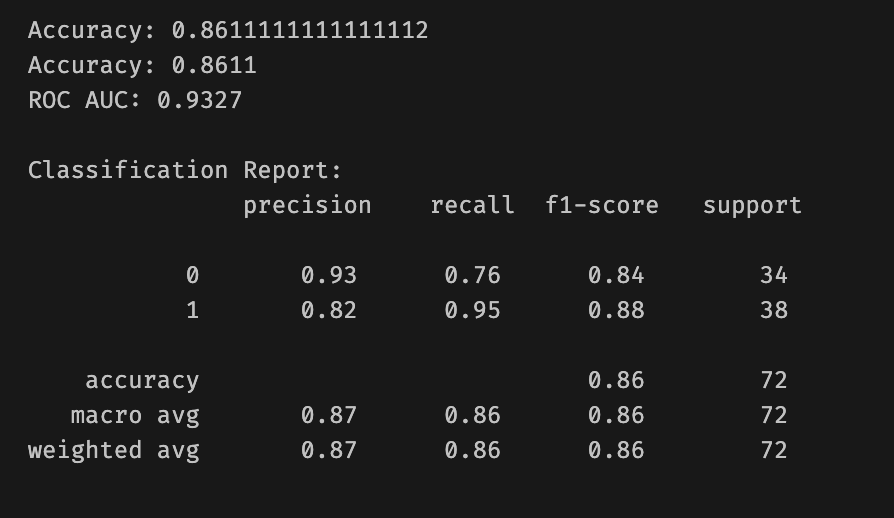
\includegraphics[width=1\textwidth,height=\textheight]{figures/linear_result_imagined.png}

\subcaption{\label{}(a) Imagined Movements}
\end{minipage}%
%
\begin{minipage}{0.50\linewidth}

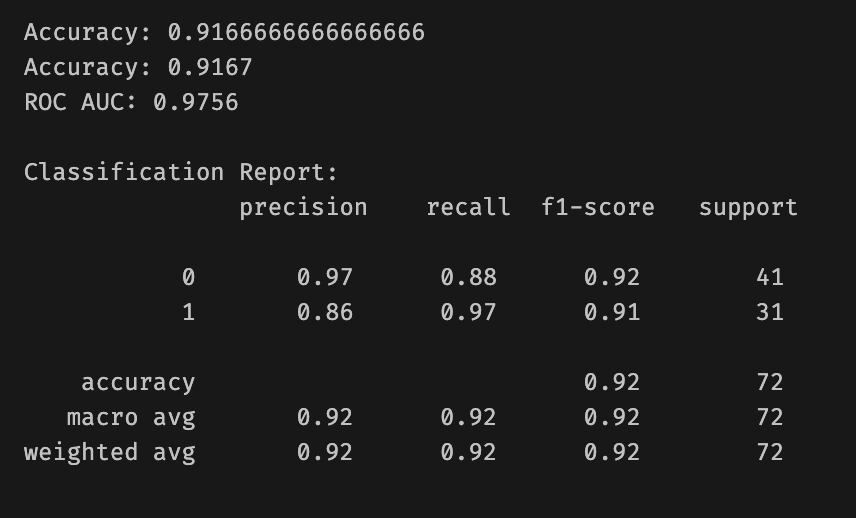
\includegraphics[width=1\textwidth,height=\textheight]{figures/linear_result_overt.png}

\subcaption{\label{}(b) Overt Movements}
\end{minipage}%

\caption{\label{fig-linearSVM}Linear SVM performance metrics for (a)
imagined versus (b) overt movements, showing classification accuracy,
ROC-AUC, and classification report.}

\end{figure}%

\subsubsection{Weight Analysis and
Interpretation}\label{weight-analysis-and-interpretation}

The weight vector \(\mathbf{w} \in \mathbb{R}^{204}\) from the trained
linear SVM was analyzed to interpret spatial channel importance. The
204-element vector was split into x-gradient (\texttt{W\_x}) and
y-gradient (\texttt{W\_y}) components, and a per-electrode magnitude was
computed:

\[
W_k = \sqrt{w_{2k-1}^2 + w_{2k}^2}, \quad k = 1, \dots, 102
\]

These magnitudes were plotted to visualize the influence of each
electrode, such as on Figure~\ref{fig-linearSVM-weights}.

\begin{figure}

\centering{

\begin{figure}
\centering
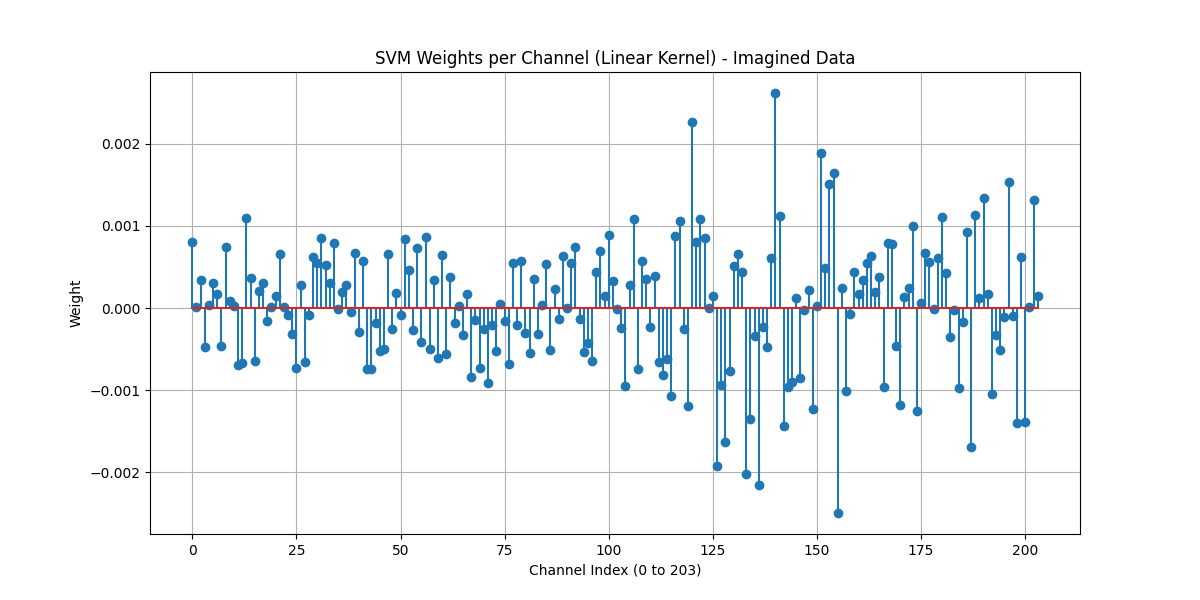
\includegraphics[width=0.9\textwidth,height=\textheight]{figures/linearSVM/linearSVM_weights_perChannel_imagined.png}
\caption{(a) Imagined Movements}\label{fig:linear-svm-imagined-weights}
\end{figure}

\begin{figure}
\centering
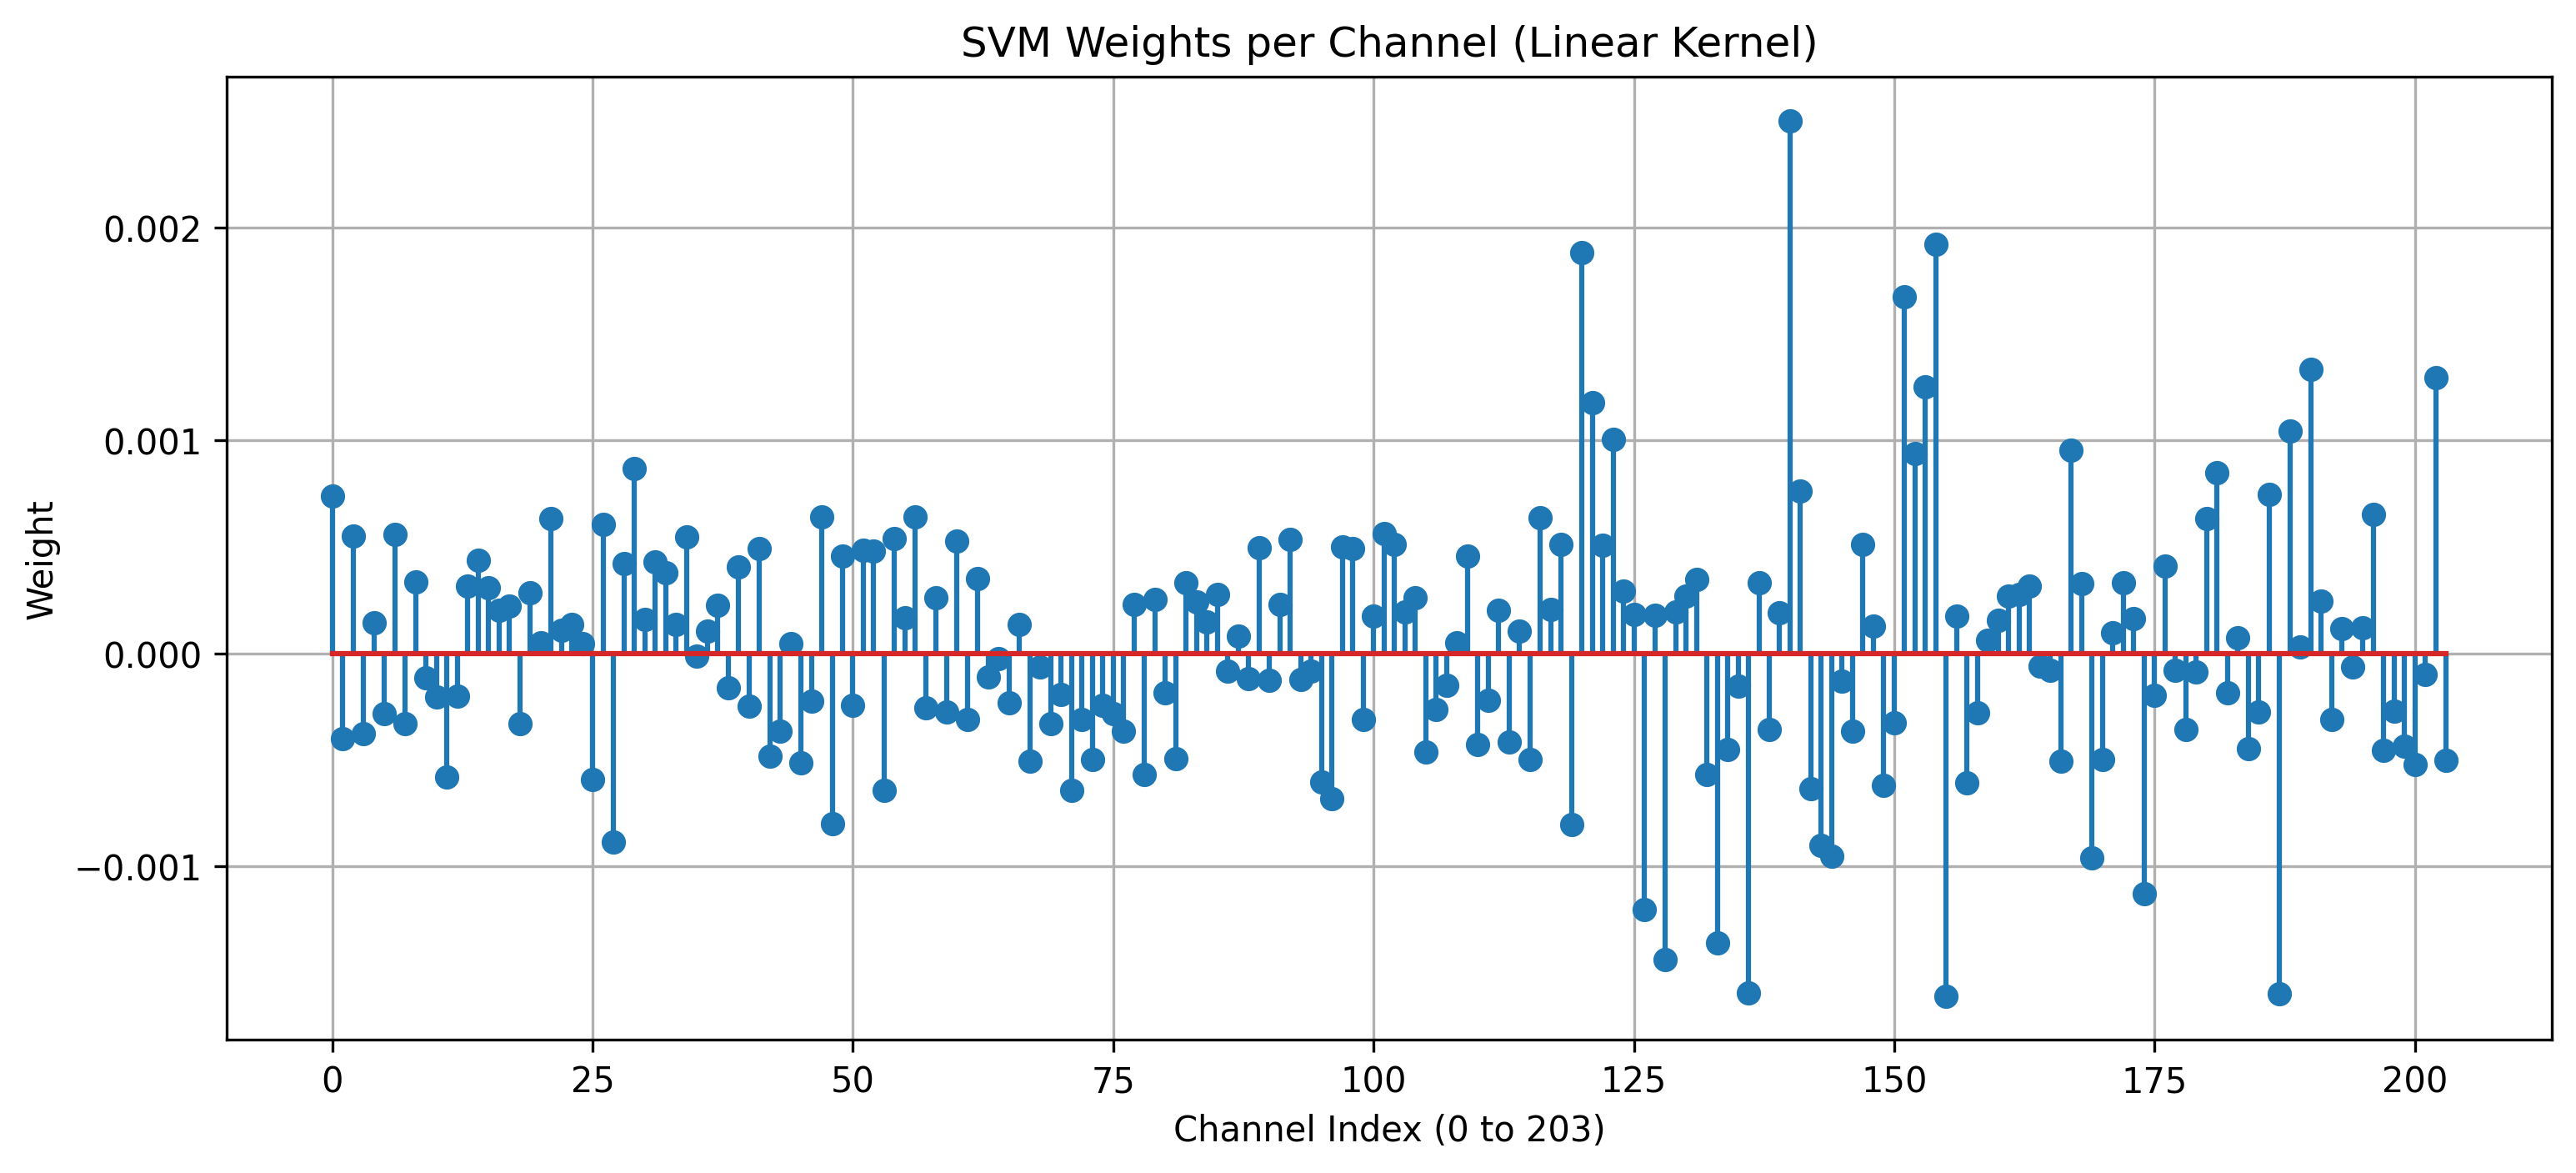
\includegraphics[width=0.8\textwidth,height=\textheight]{figures/linearSVM/linearSVM_weights_per_channel_real.png}
\caption{(b) Overt Movements}\label{fig:linear-svm-overt-weights}
\end{figure}

}

\caption{\label{fig-linearSVM-weights}Linear SVM weight magnitudes for
(a) imagined versus (b) overt movements, showing the relative importance
of each electrode in the classification decision. Topographic maps
display normalized weights (μV) across scalp regions, with red
indicating positive contribution and blue indicating negative
contribution to classification.}

\end{figure}%

\subsubsection{Topographic Mapping}\label{topographic-mapping}

To understand spatial patterns, electrode positions from
\texttt{BCIsensor\_xy.csv} were scaled and mapped to a topographic head
model using MNE-Python. The magnitude values \texttt{W\_mag} were
plotted using MNE's \texttt{plot\_topomap} function.

\begin{itemize}
\tightlist
\item
  Topomaps provided intuitive spatial distribution of informative
  channels.
\item
  Interpolated heatmaps were also generated using
  \texttt{scipy.interpolate.griddata} to visualize gradients.
\end{itemize}

In order words, we can visualize where is located the most important
electrodes for the classification of the imagined and overt movements.
The topographic maps were generated using MNE-Python's
\texttt{plot\_topomap} function, which allows for intuitive spatial
distribution of informative channels. The topomaps are shown in
Figure~\ref{fig-topomap}.

\begin{figure}

\centering{

\begin{figure}
\centering
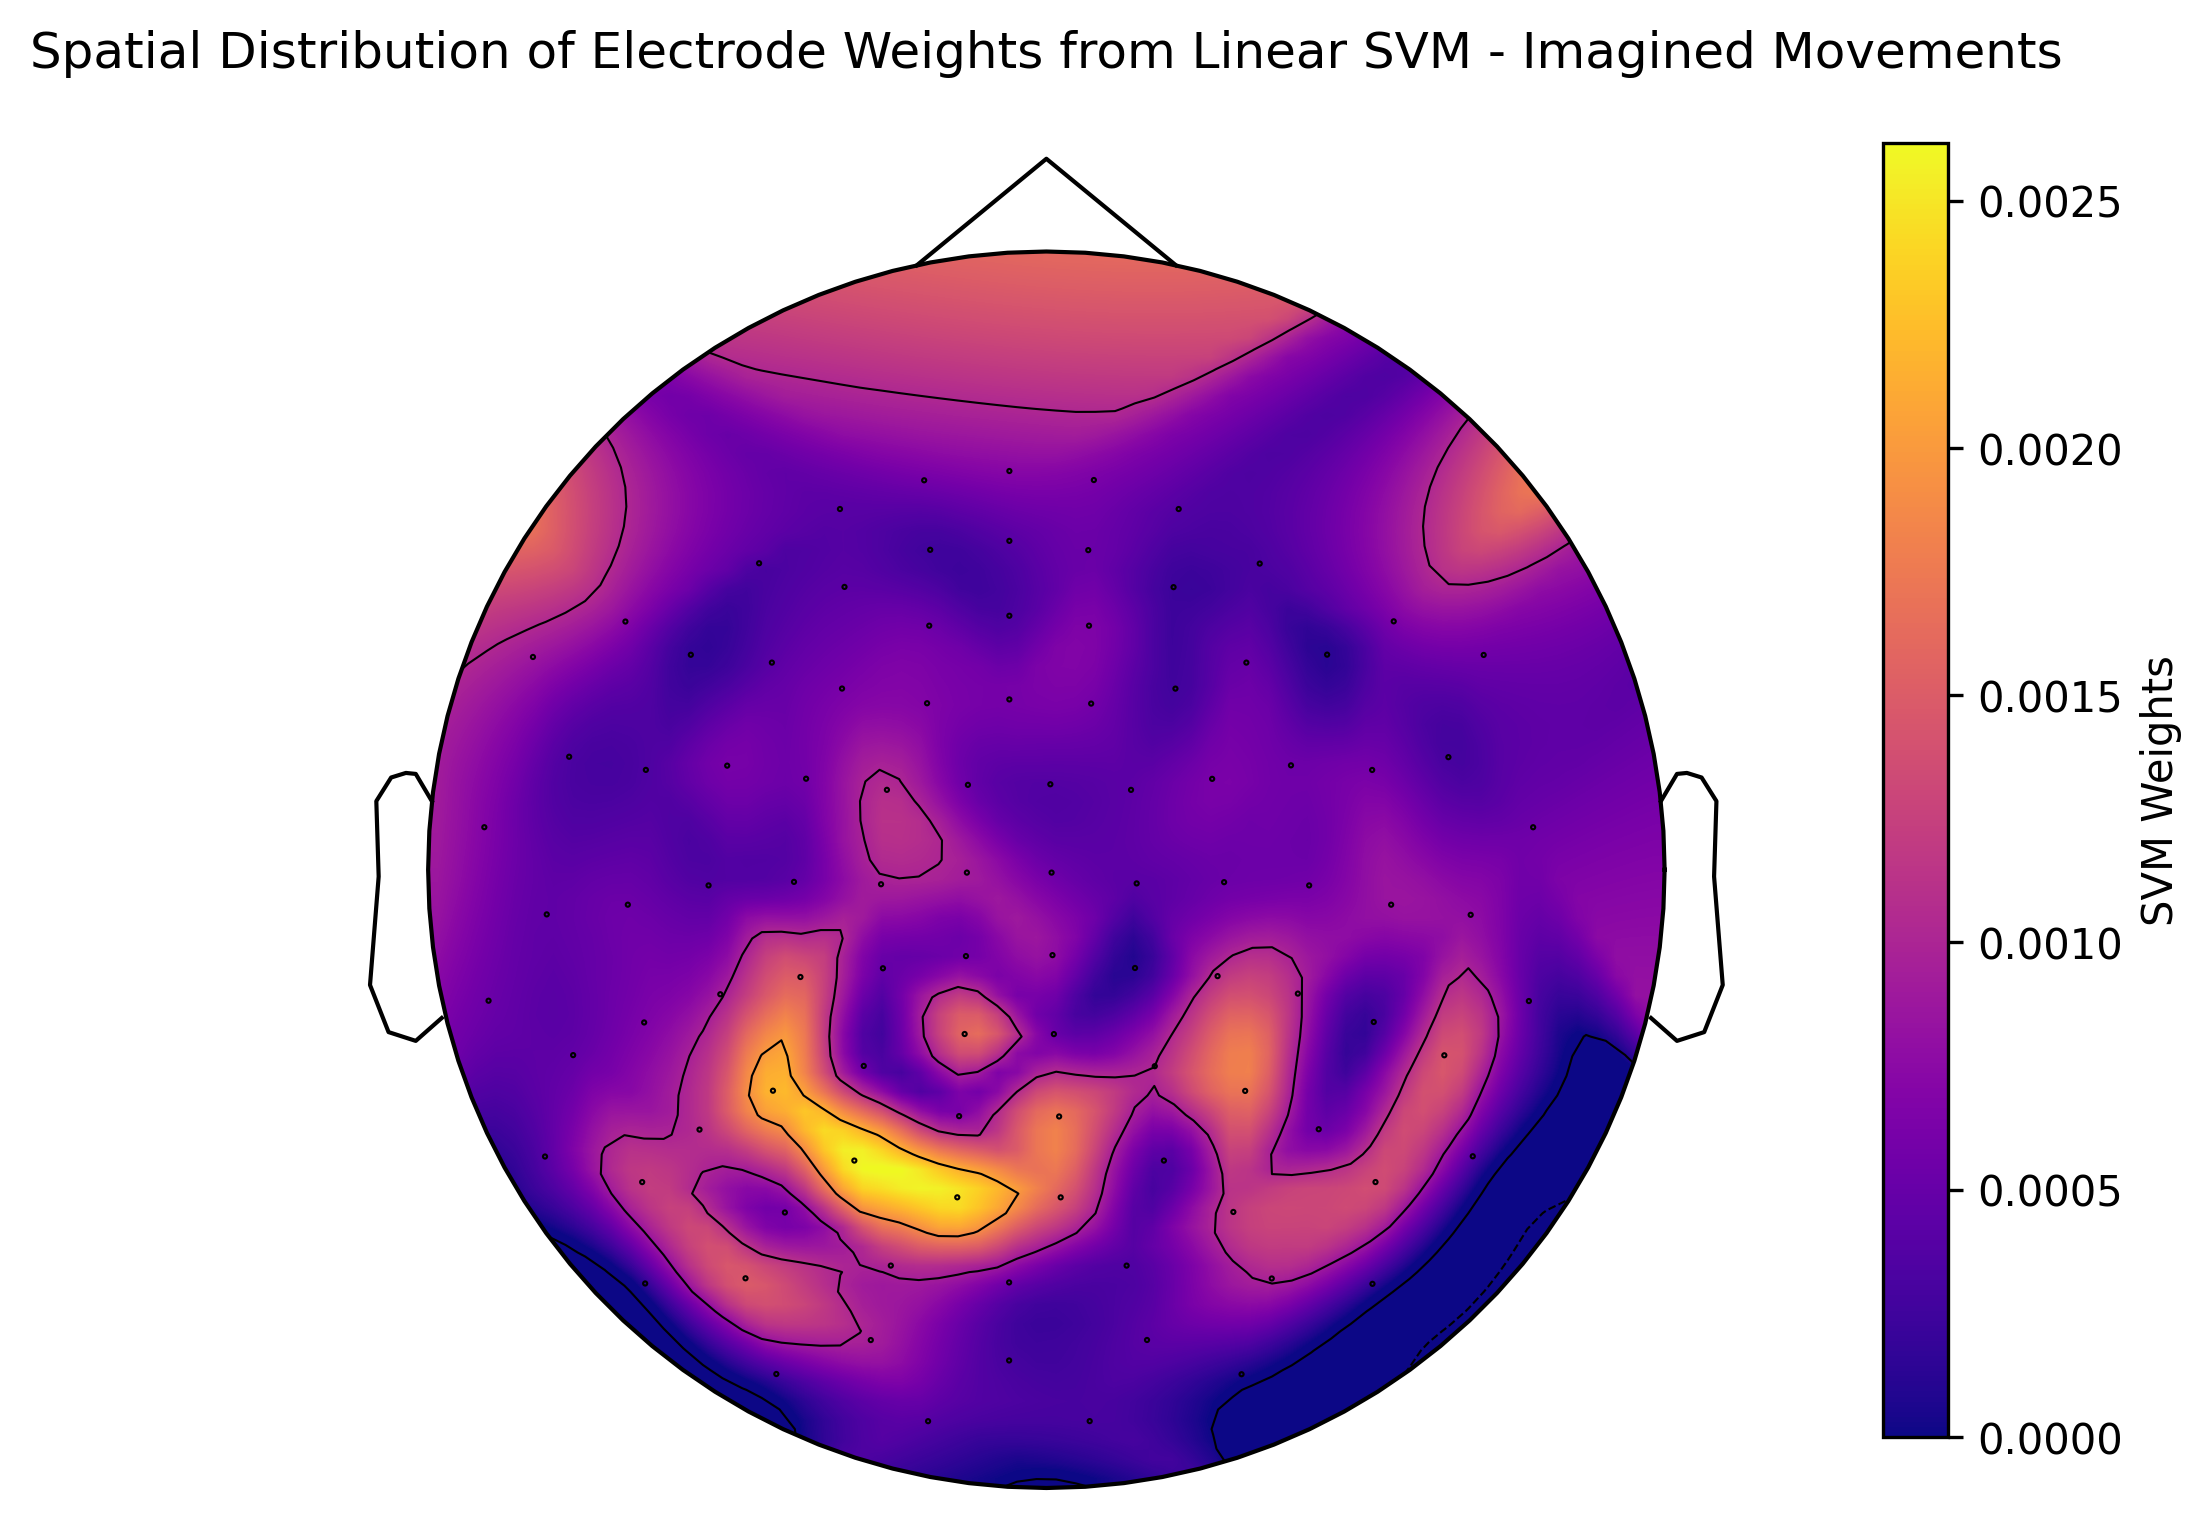
\includegraphics[width=1\textwidth,height=\textheight]{figures/linearSVM/topomap_imagined_movements_extrapolated.png}
\caption{(a) Imagined Movements
(Extrapolated)}\label{fig:topomap-imagined-extrapolated}
\end{figure}

\begin{figure}
\centering
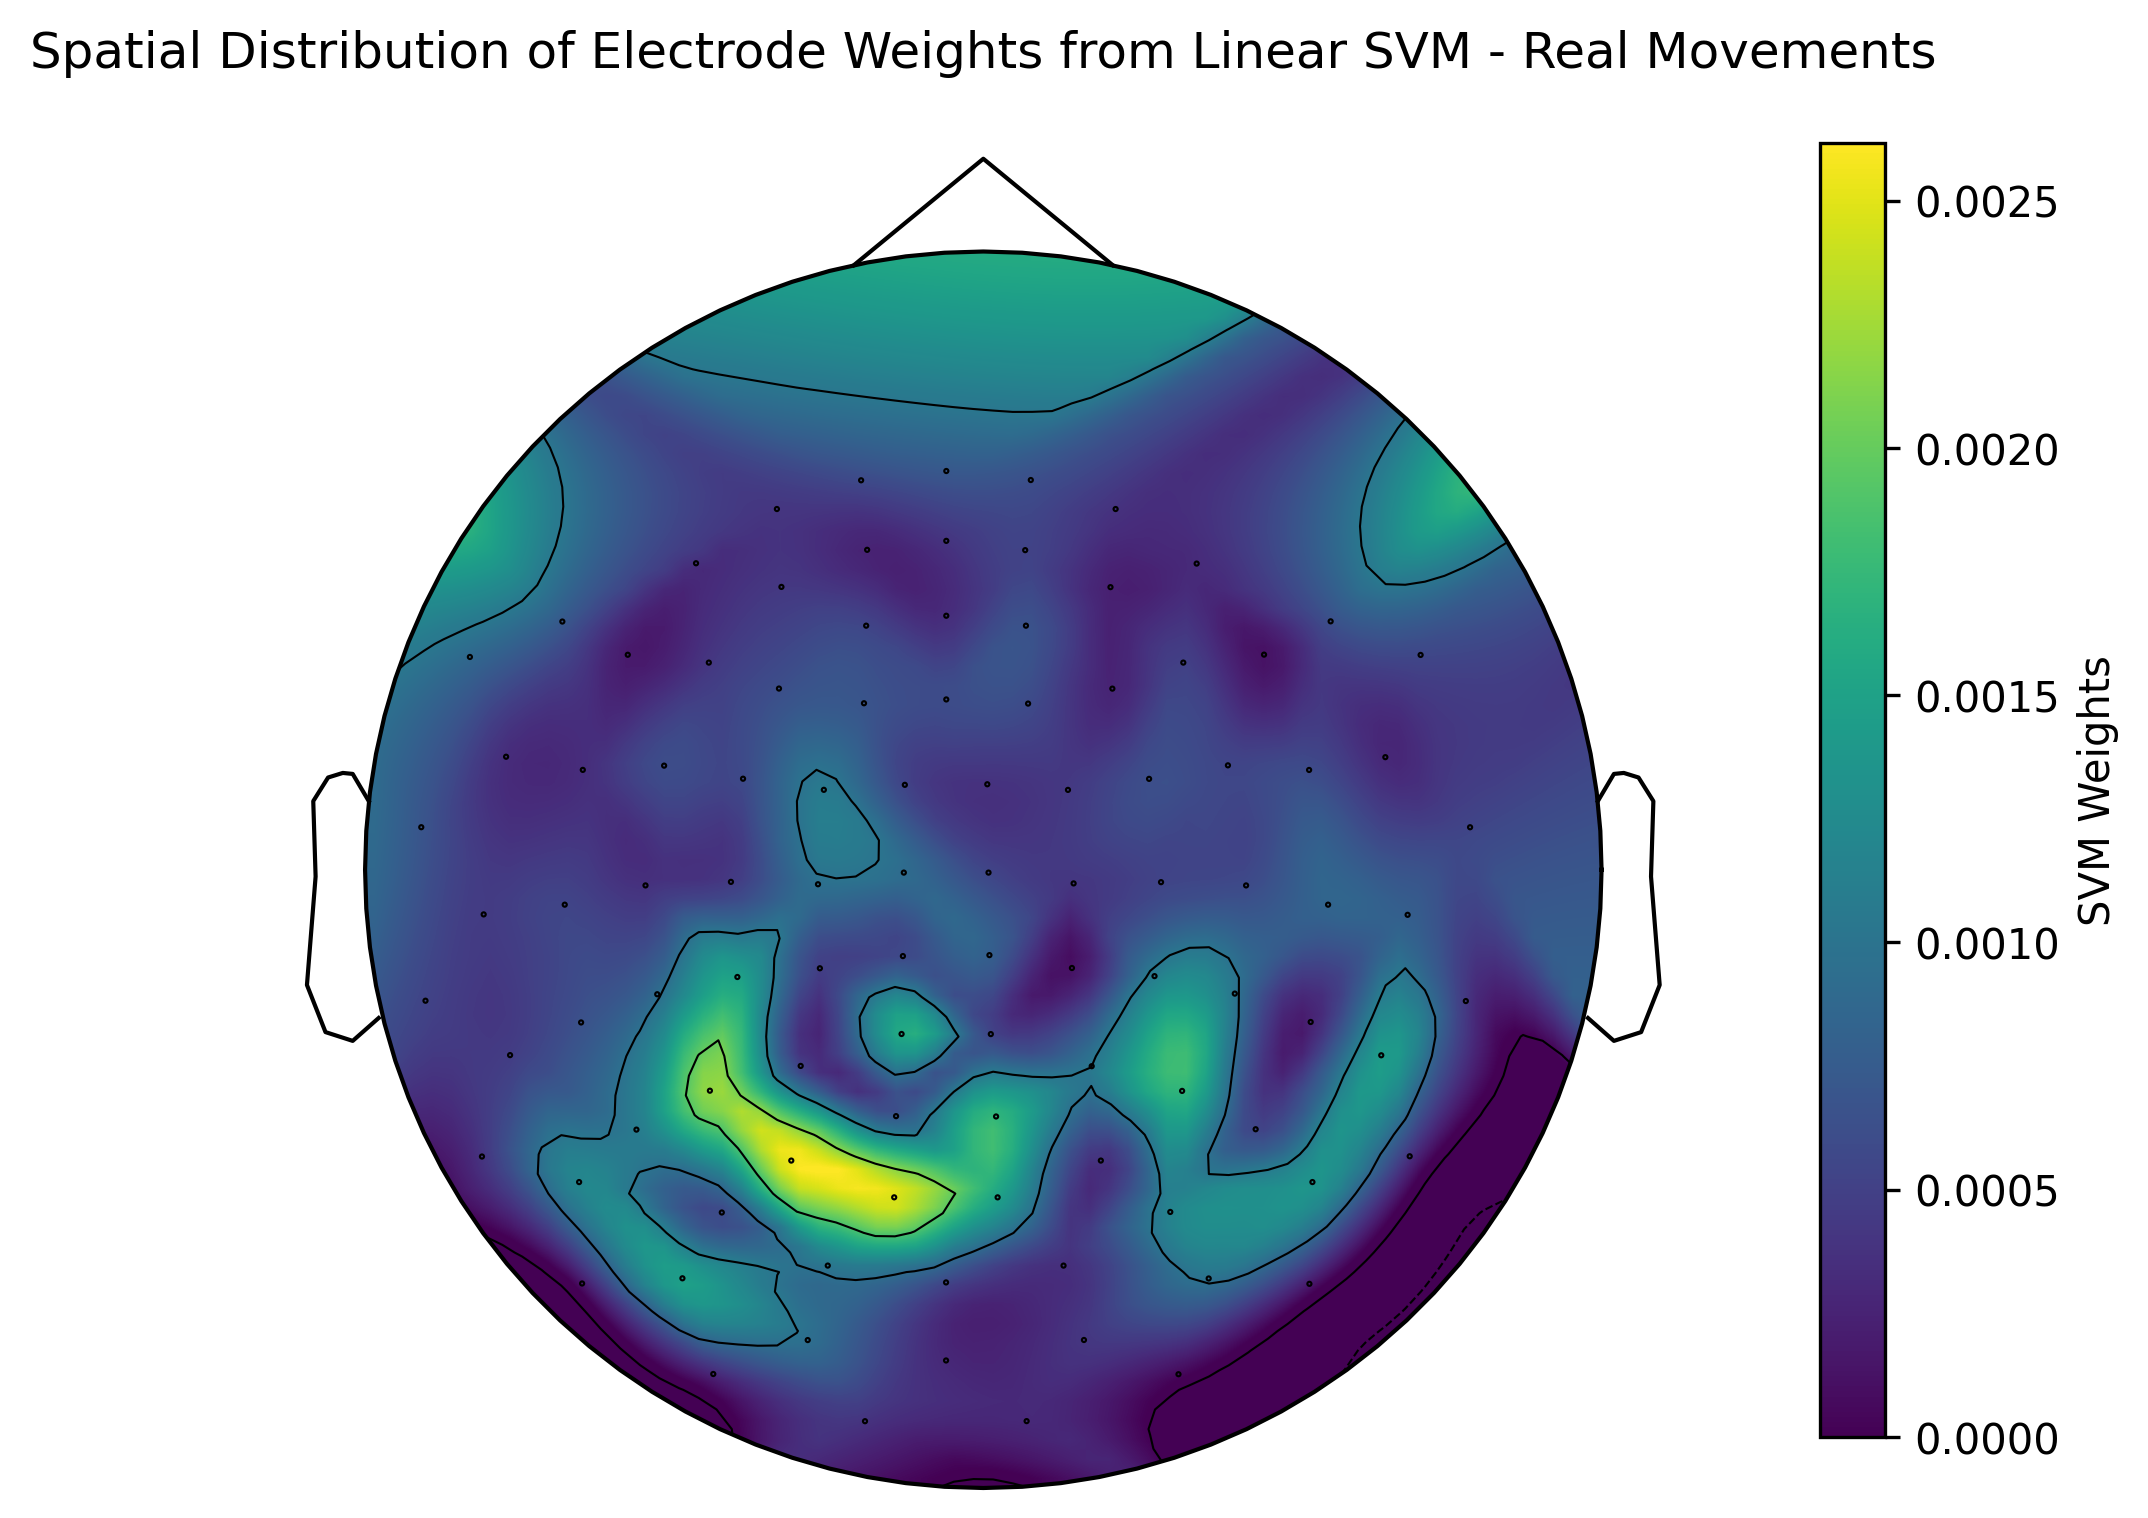
\includegraphics[width=1\textwidth,height=\textheight]{figures/linearSVM/topomap_real_movements_extrapolated_linearSVM.png}
\caption{(b) Overt Movements
(Extrapolated)}\label{fig:topomap-overt-extrapolated}
\end{figure}

\begin{figure}
\centering
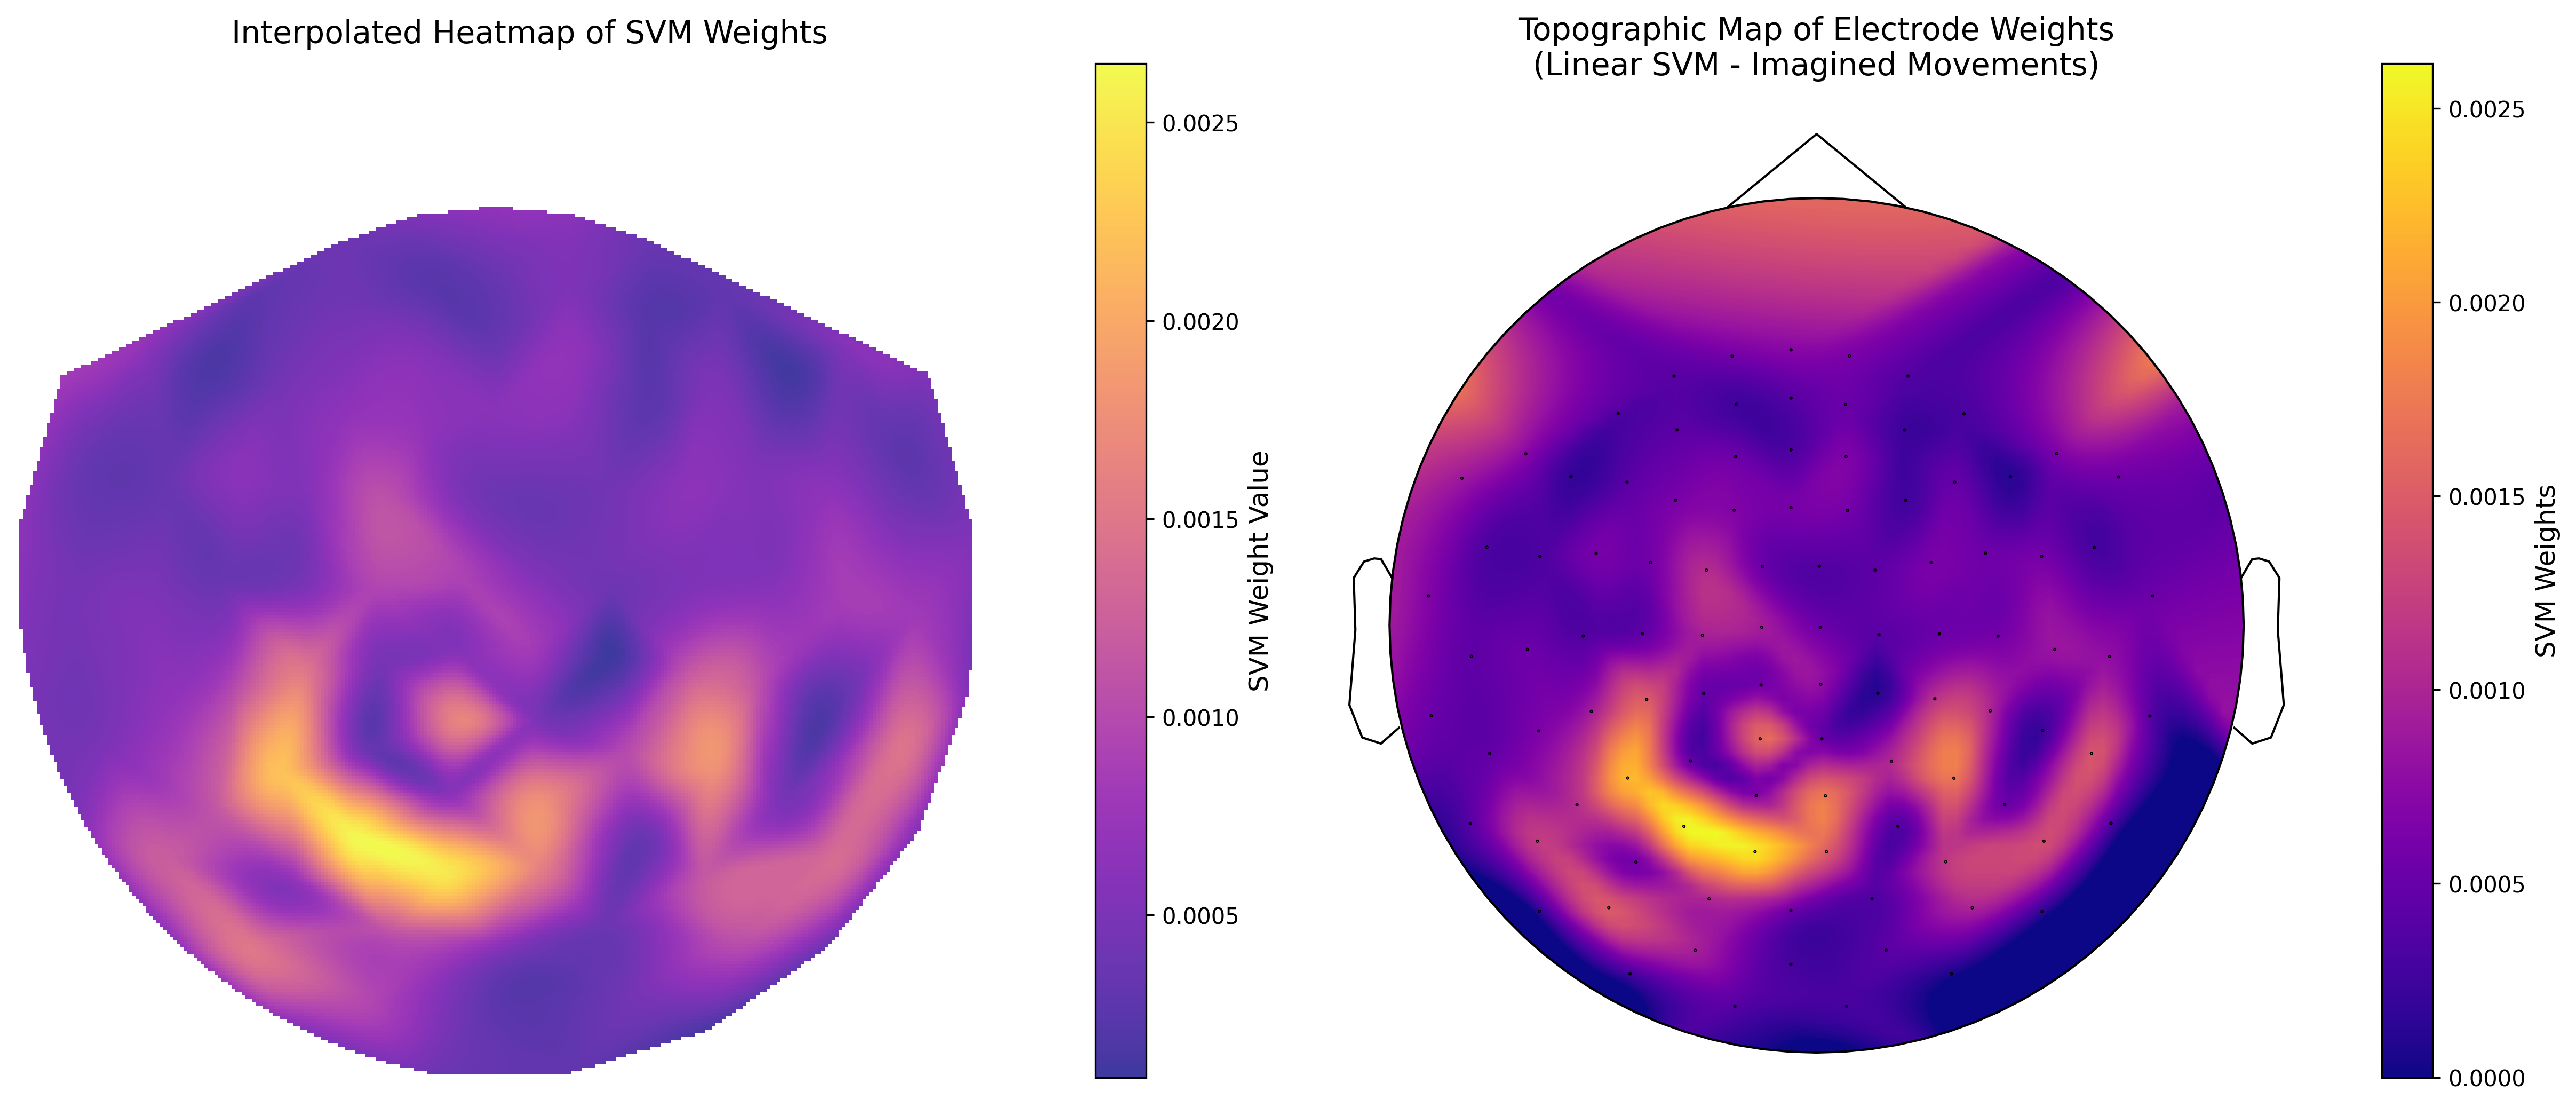
\includegraphics[width=0.95\textwidth,height=\textheight]{figures/linearSVM/topomap_imagined_movements_interpolated_complete.png}
\caption{(c) Imagined Movements
(Interpolated)}\label{fig:topomap-imagined-interpolated}
\end{figure}

\begin{figure}
\centering
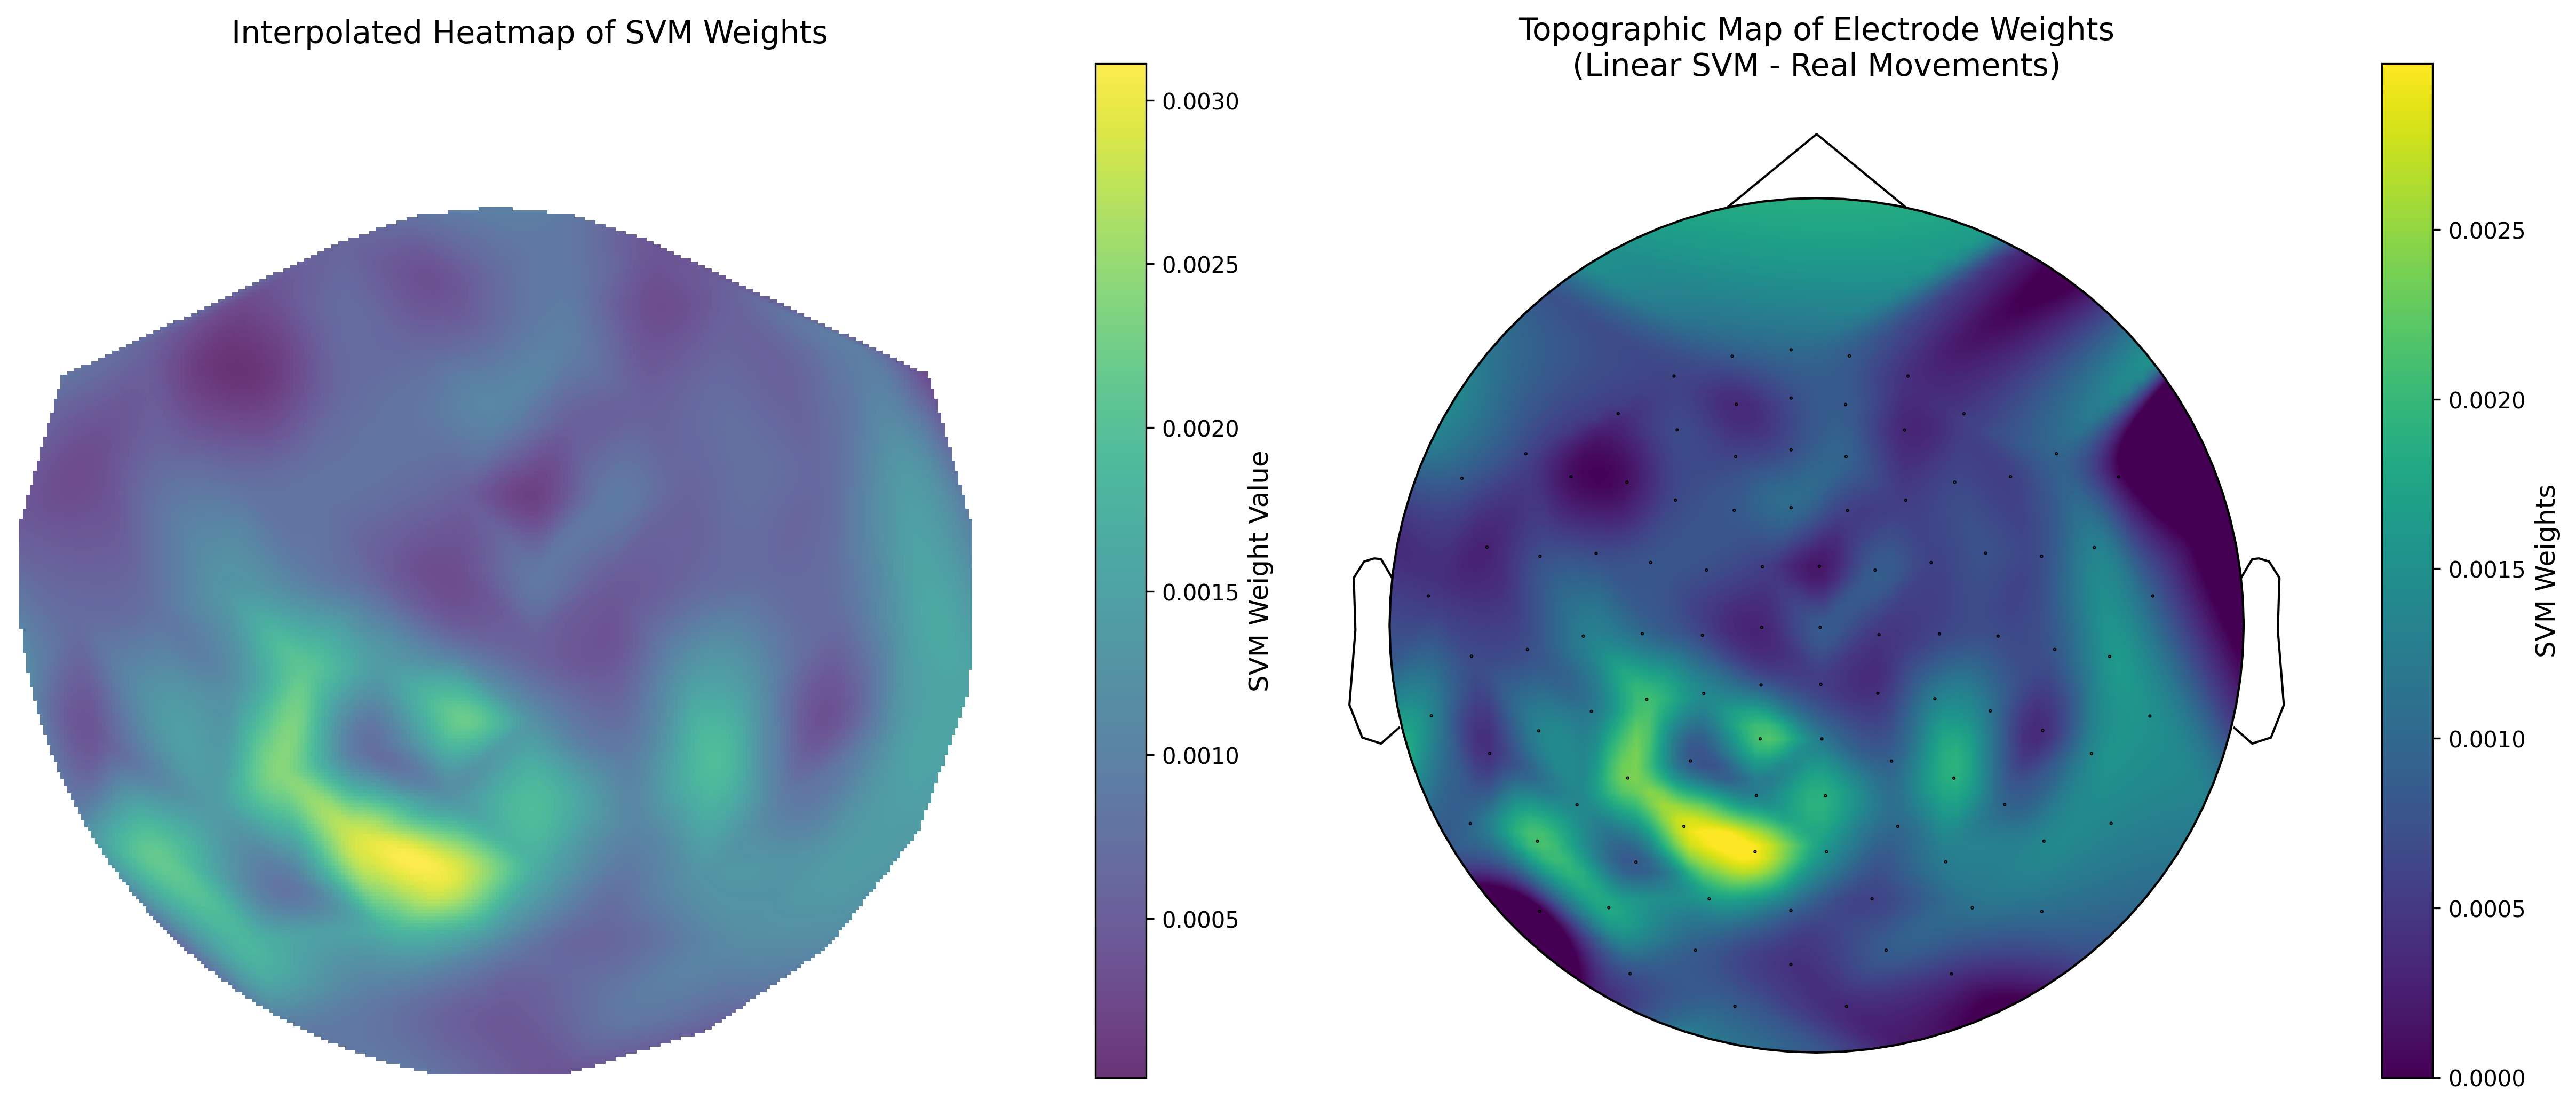
\includegraphics[width=0.95\textwidth,height=\textheight]{figures/linearSVM/topomap_real_movements_interpolated_complete_linearSVM.png}
\caption{(d) Overt Movements
(Interpolated)}\label{fig:topomap-overt-interpolated}
\end{figure}

}

\caption{\label{fig-topomap}Linear SVM topographic maps showing spatial
distribution of informative electrodes: (a-b) Extrapolated and (c-d)
interpolated representations for imagined versus overt movements. Warmer
colors indicate stronger positive weights, cooler colors show negative
weights in the classification decision. Color bars represent normalized
weight values.}

\end{figure}%

\subsubsection{Evaluation: Confusion Matrices and ROC
Curves}\label{evaluation-confusion-matrices-and-roc-curves}

We computed confusion matrices for both imagined and real movement
classifiers, as well as ROC curves and AUC metrics.

\textbf{Figure Placeholder:}
\texttt{confusion\_matrix\_imagined\_movements\_linearSVM.png}
\textbf{Figure Placeholder:}
\texttt{confusion\_matrix\_real\_movements\_linearSVM.png}
\textbf{Figure Placeholder:} \texttt{roc\_curves\_linear\_SVM.png}

\begin{figure}

\centering{

\begin{figure}
\centering
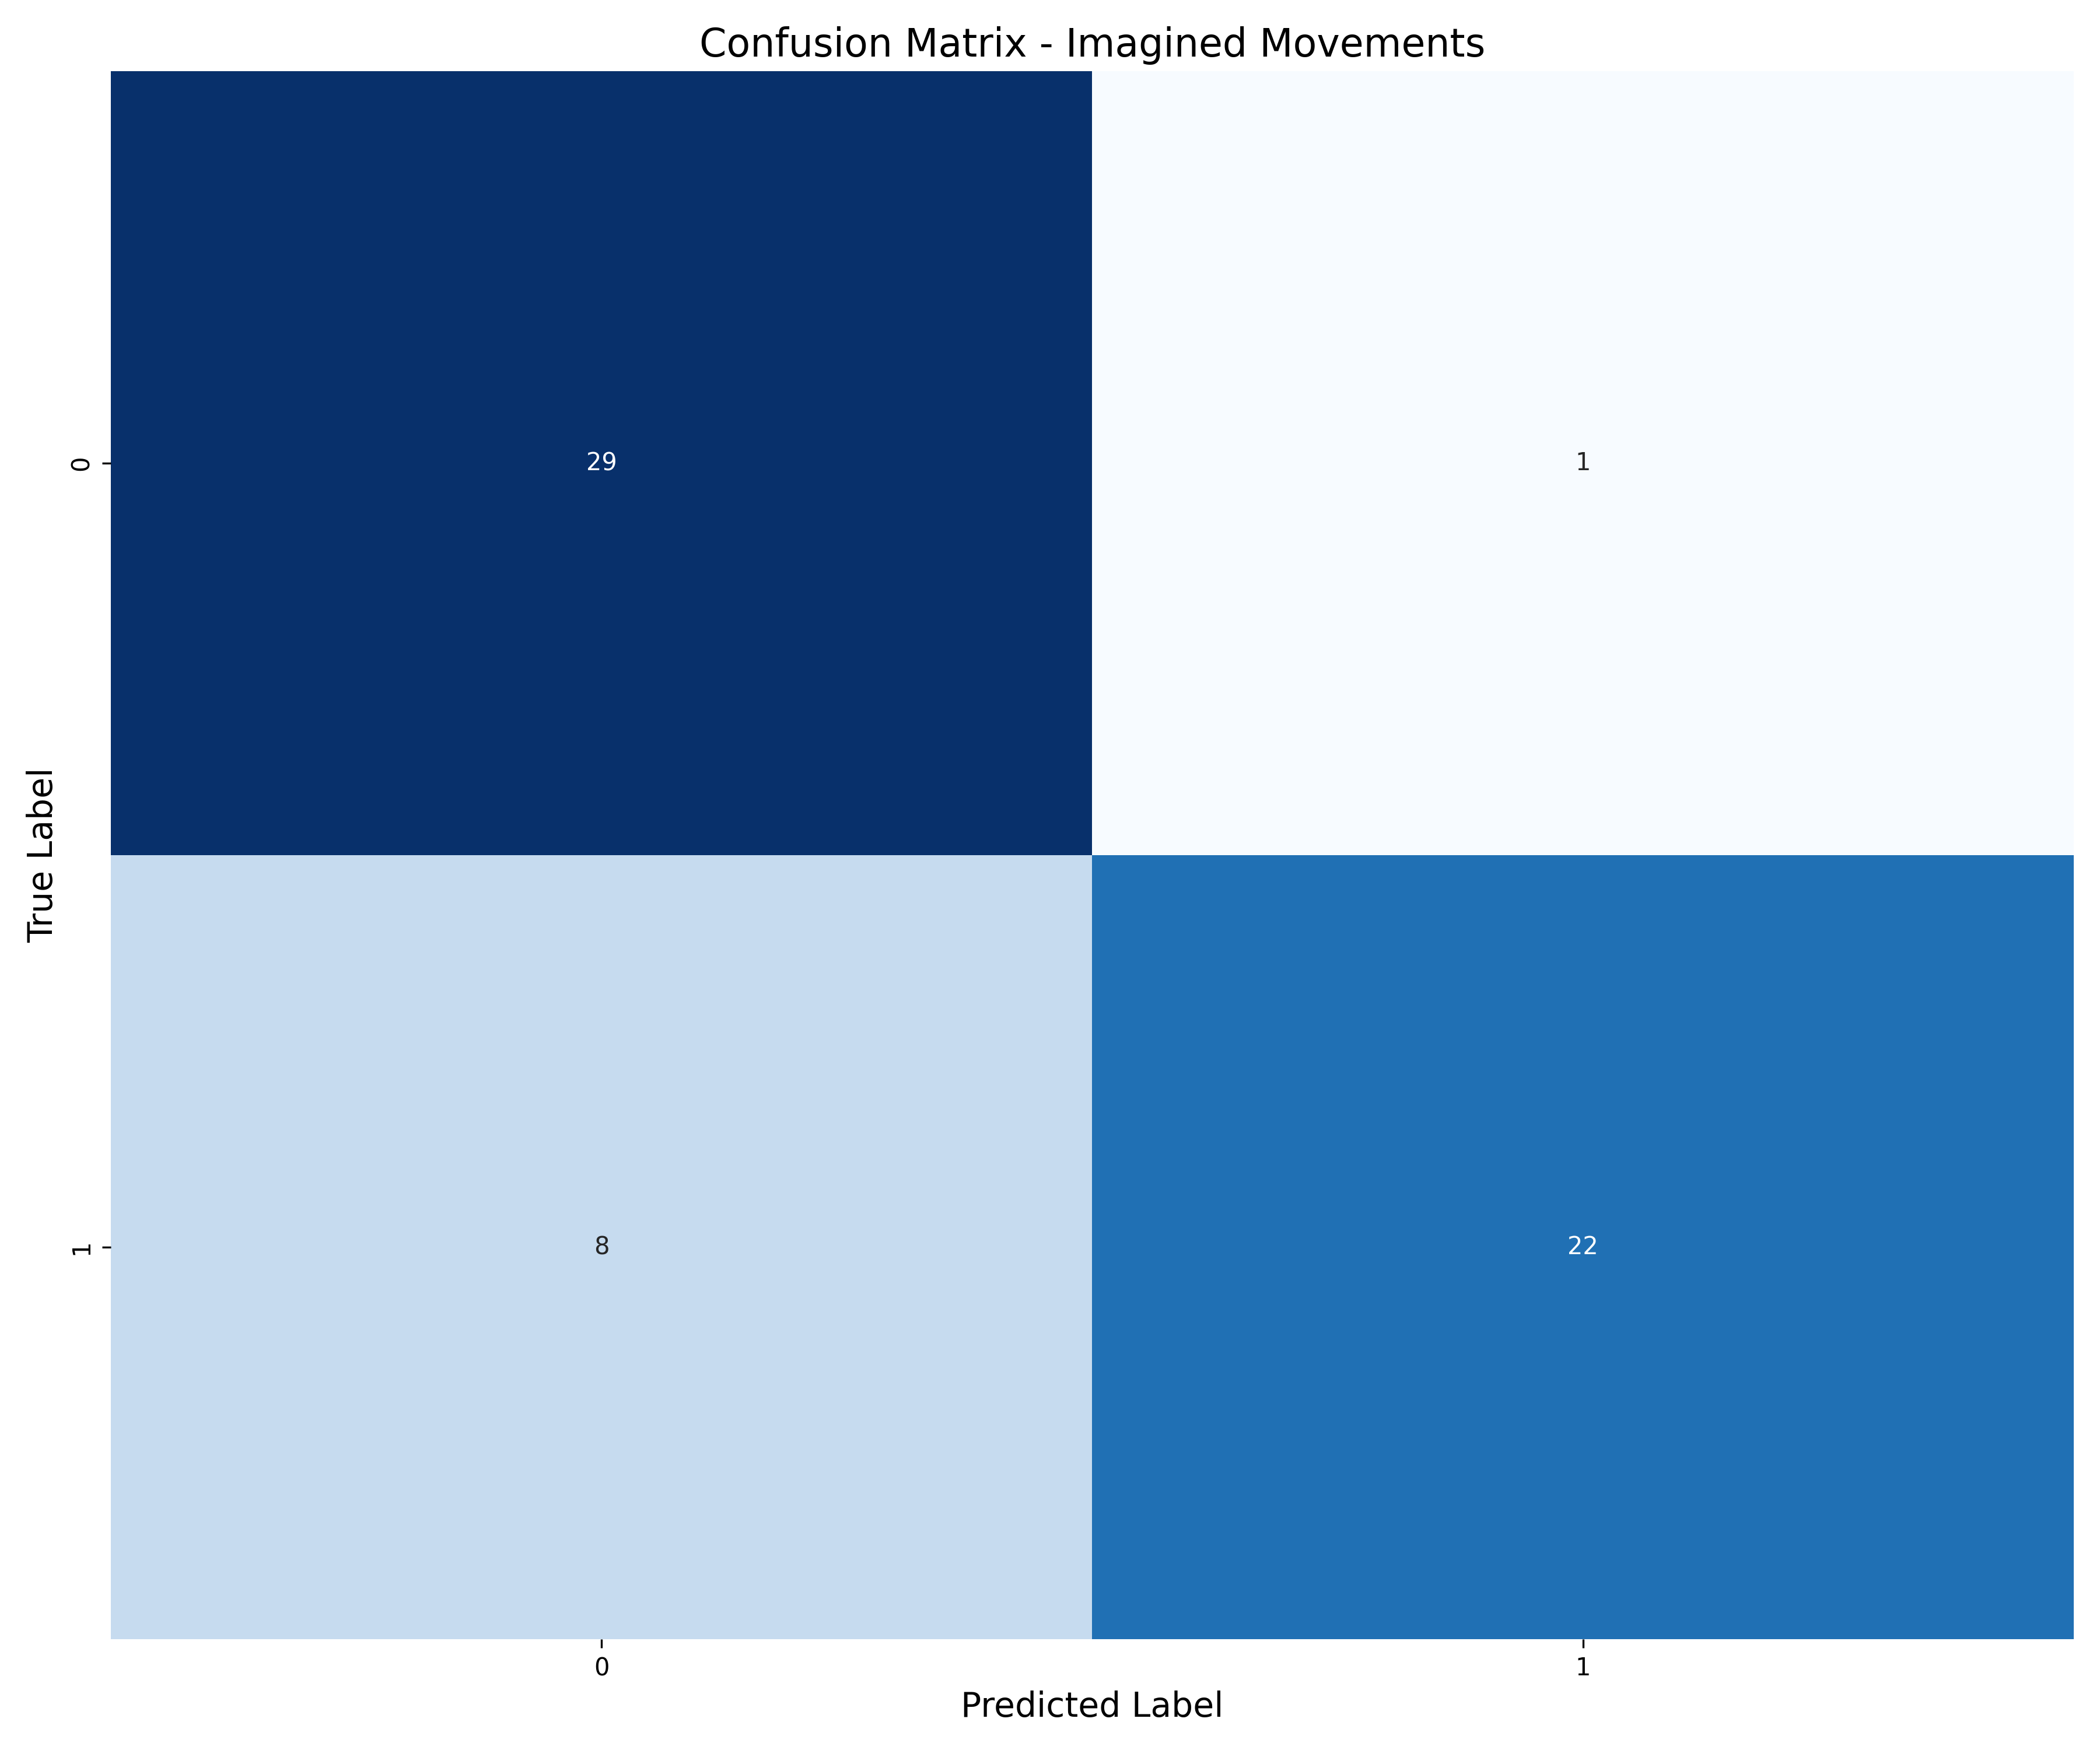
\includegraphics[width=1\textwidth,height=\textheight]{figures/linearSVM/confusion_matrix_imagined_movements_linearSVM.png}
\caption{(a) Imagined Movements}\label{fig:confusion-matrix-imagined}
\end{figure}

\begin{figure}
\centering
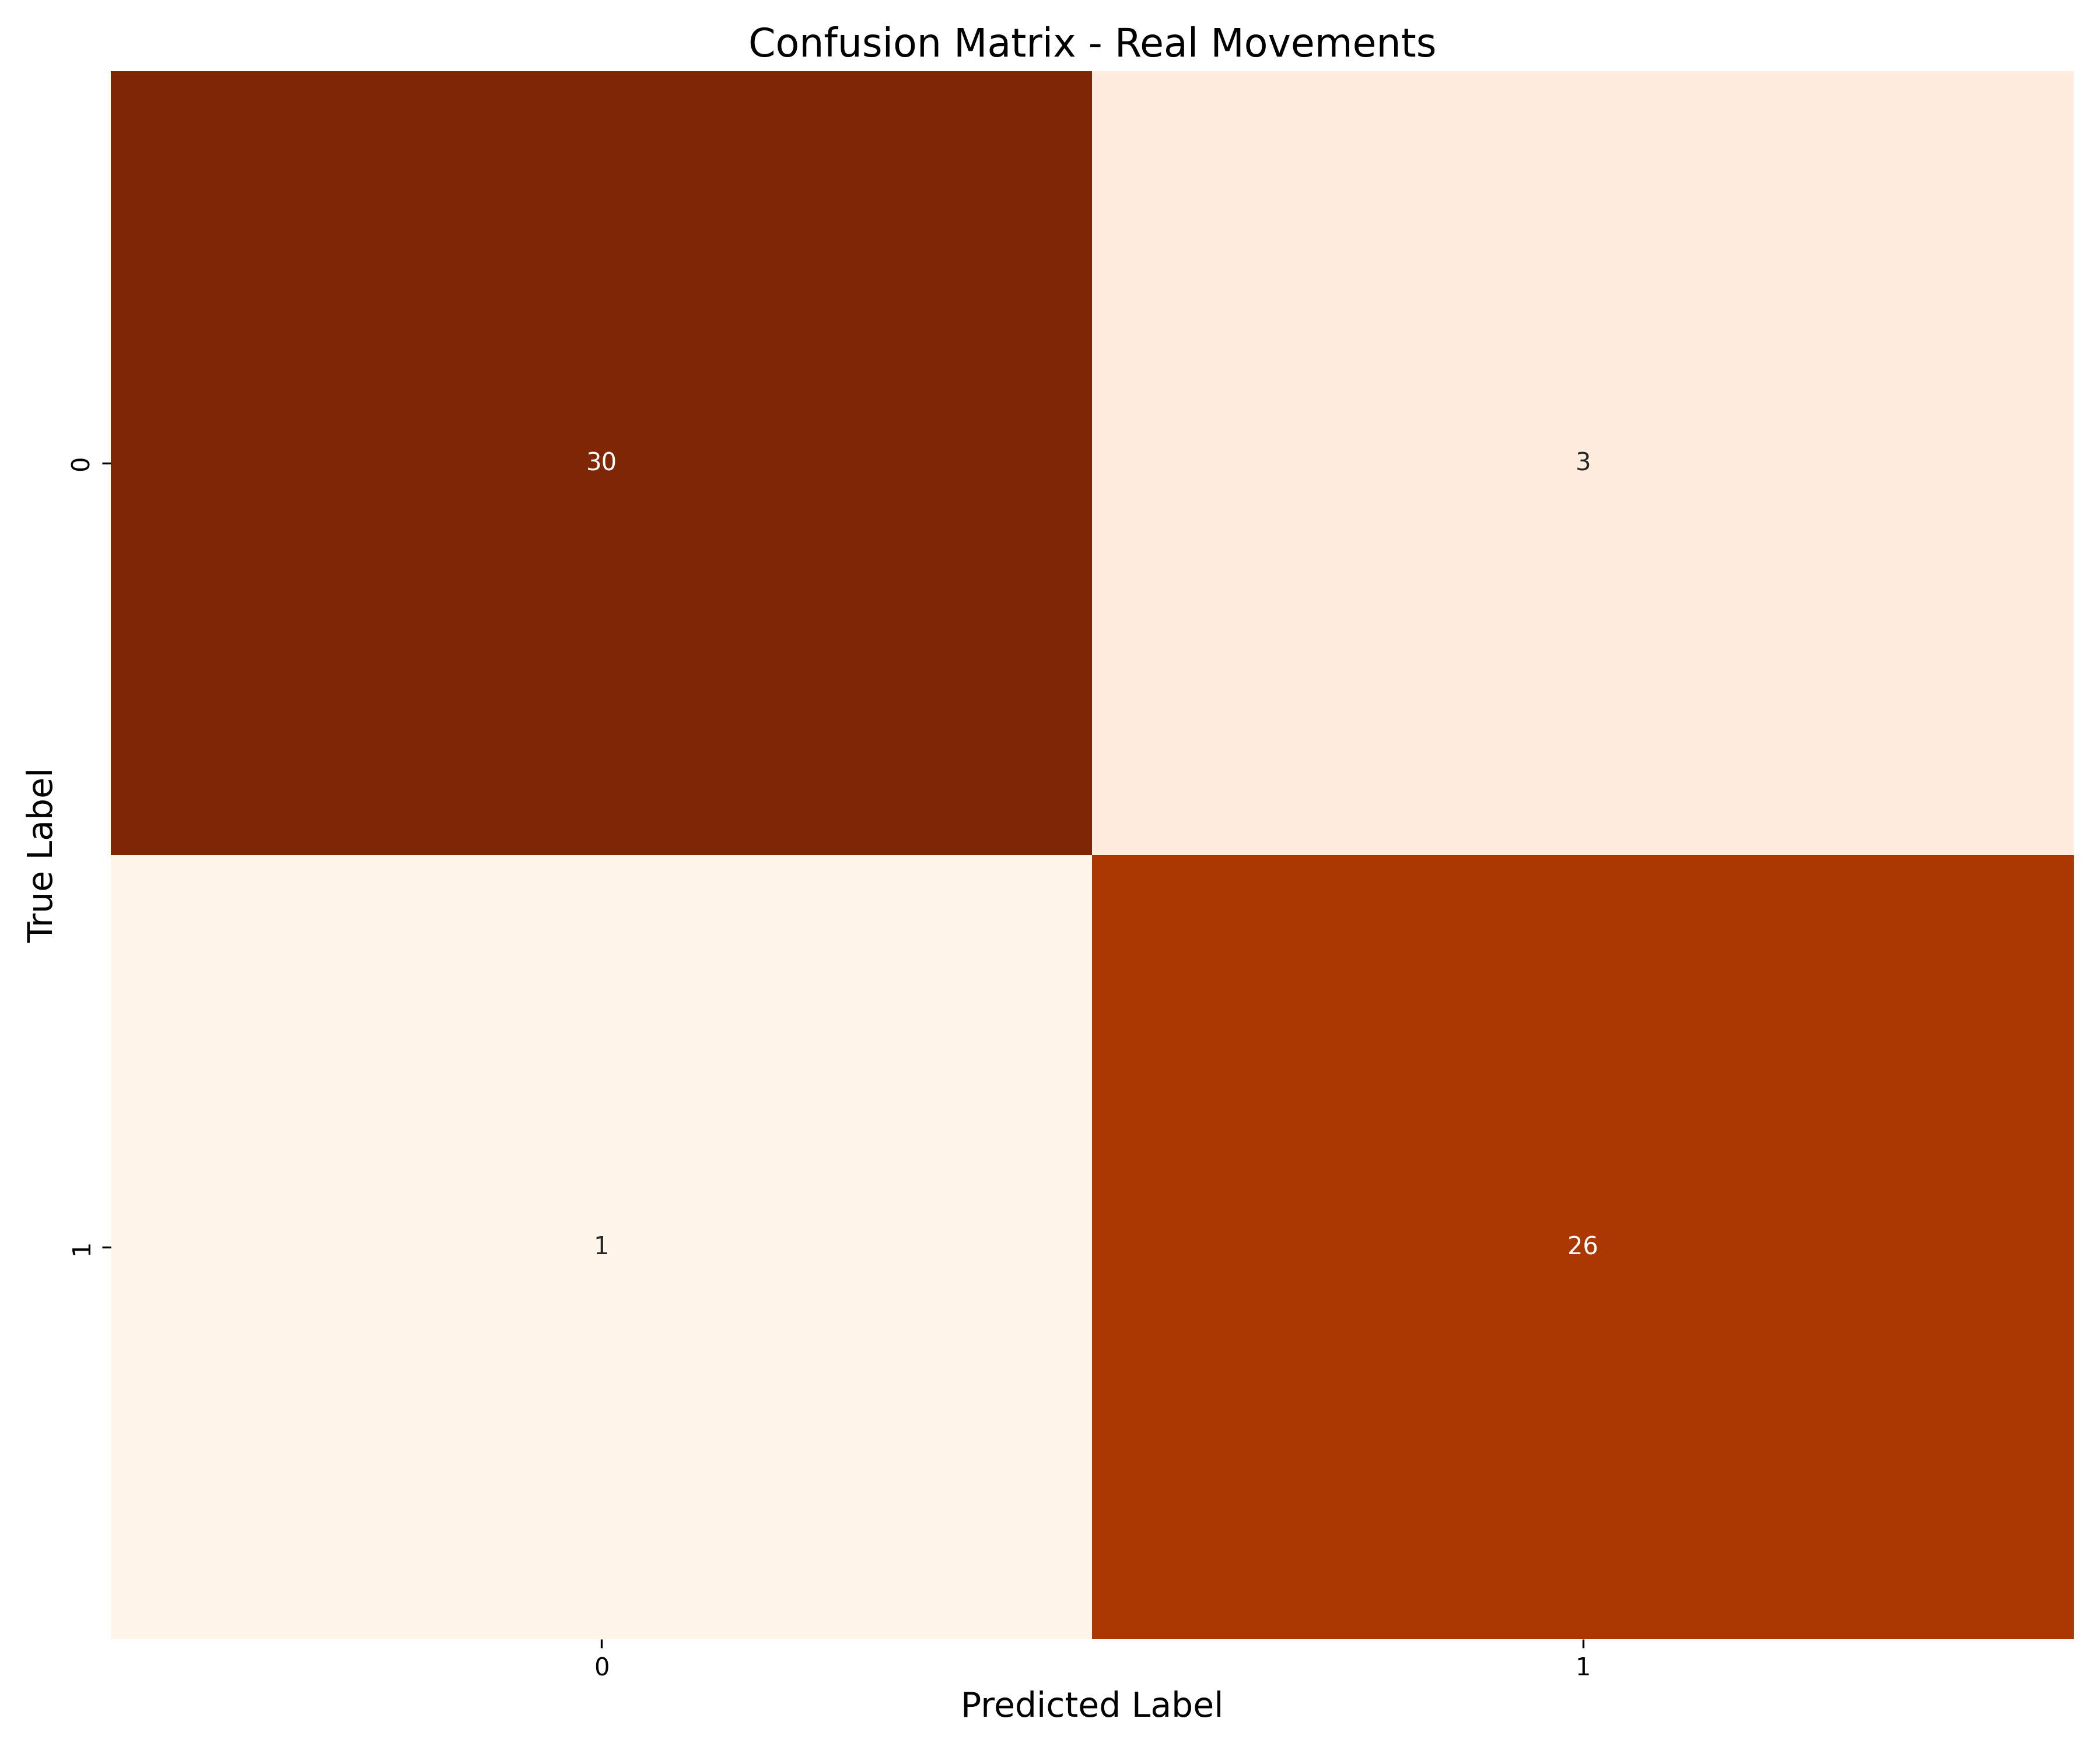
\includegraphics[width=1\textwidth,height=\textheight]{figures/linearSVM/confusion_matrix_real_movements_linearSVM.png}
\caption{(b) Overt Movements}\label{fig:confusion-matrix-overt}
\end{figure}

\begin{figure}
\centering
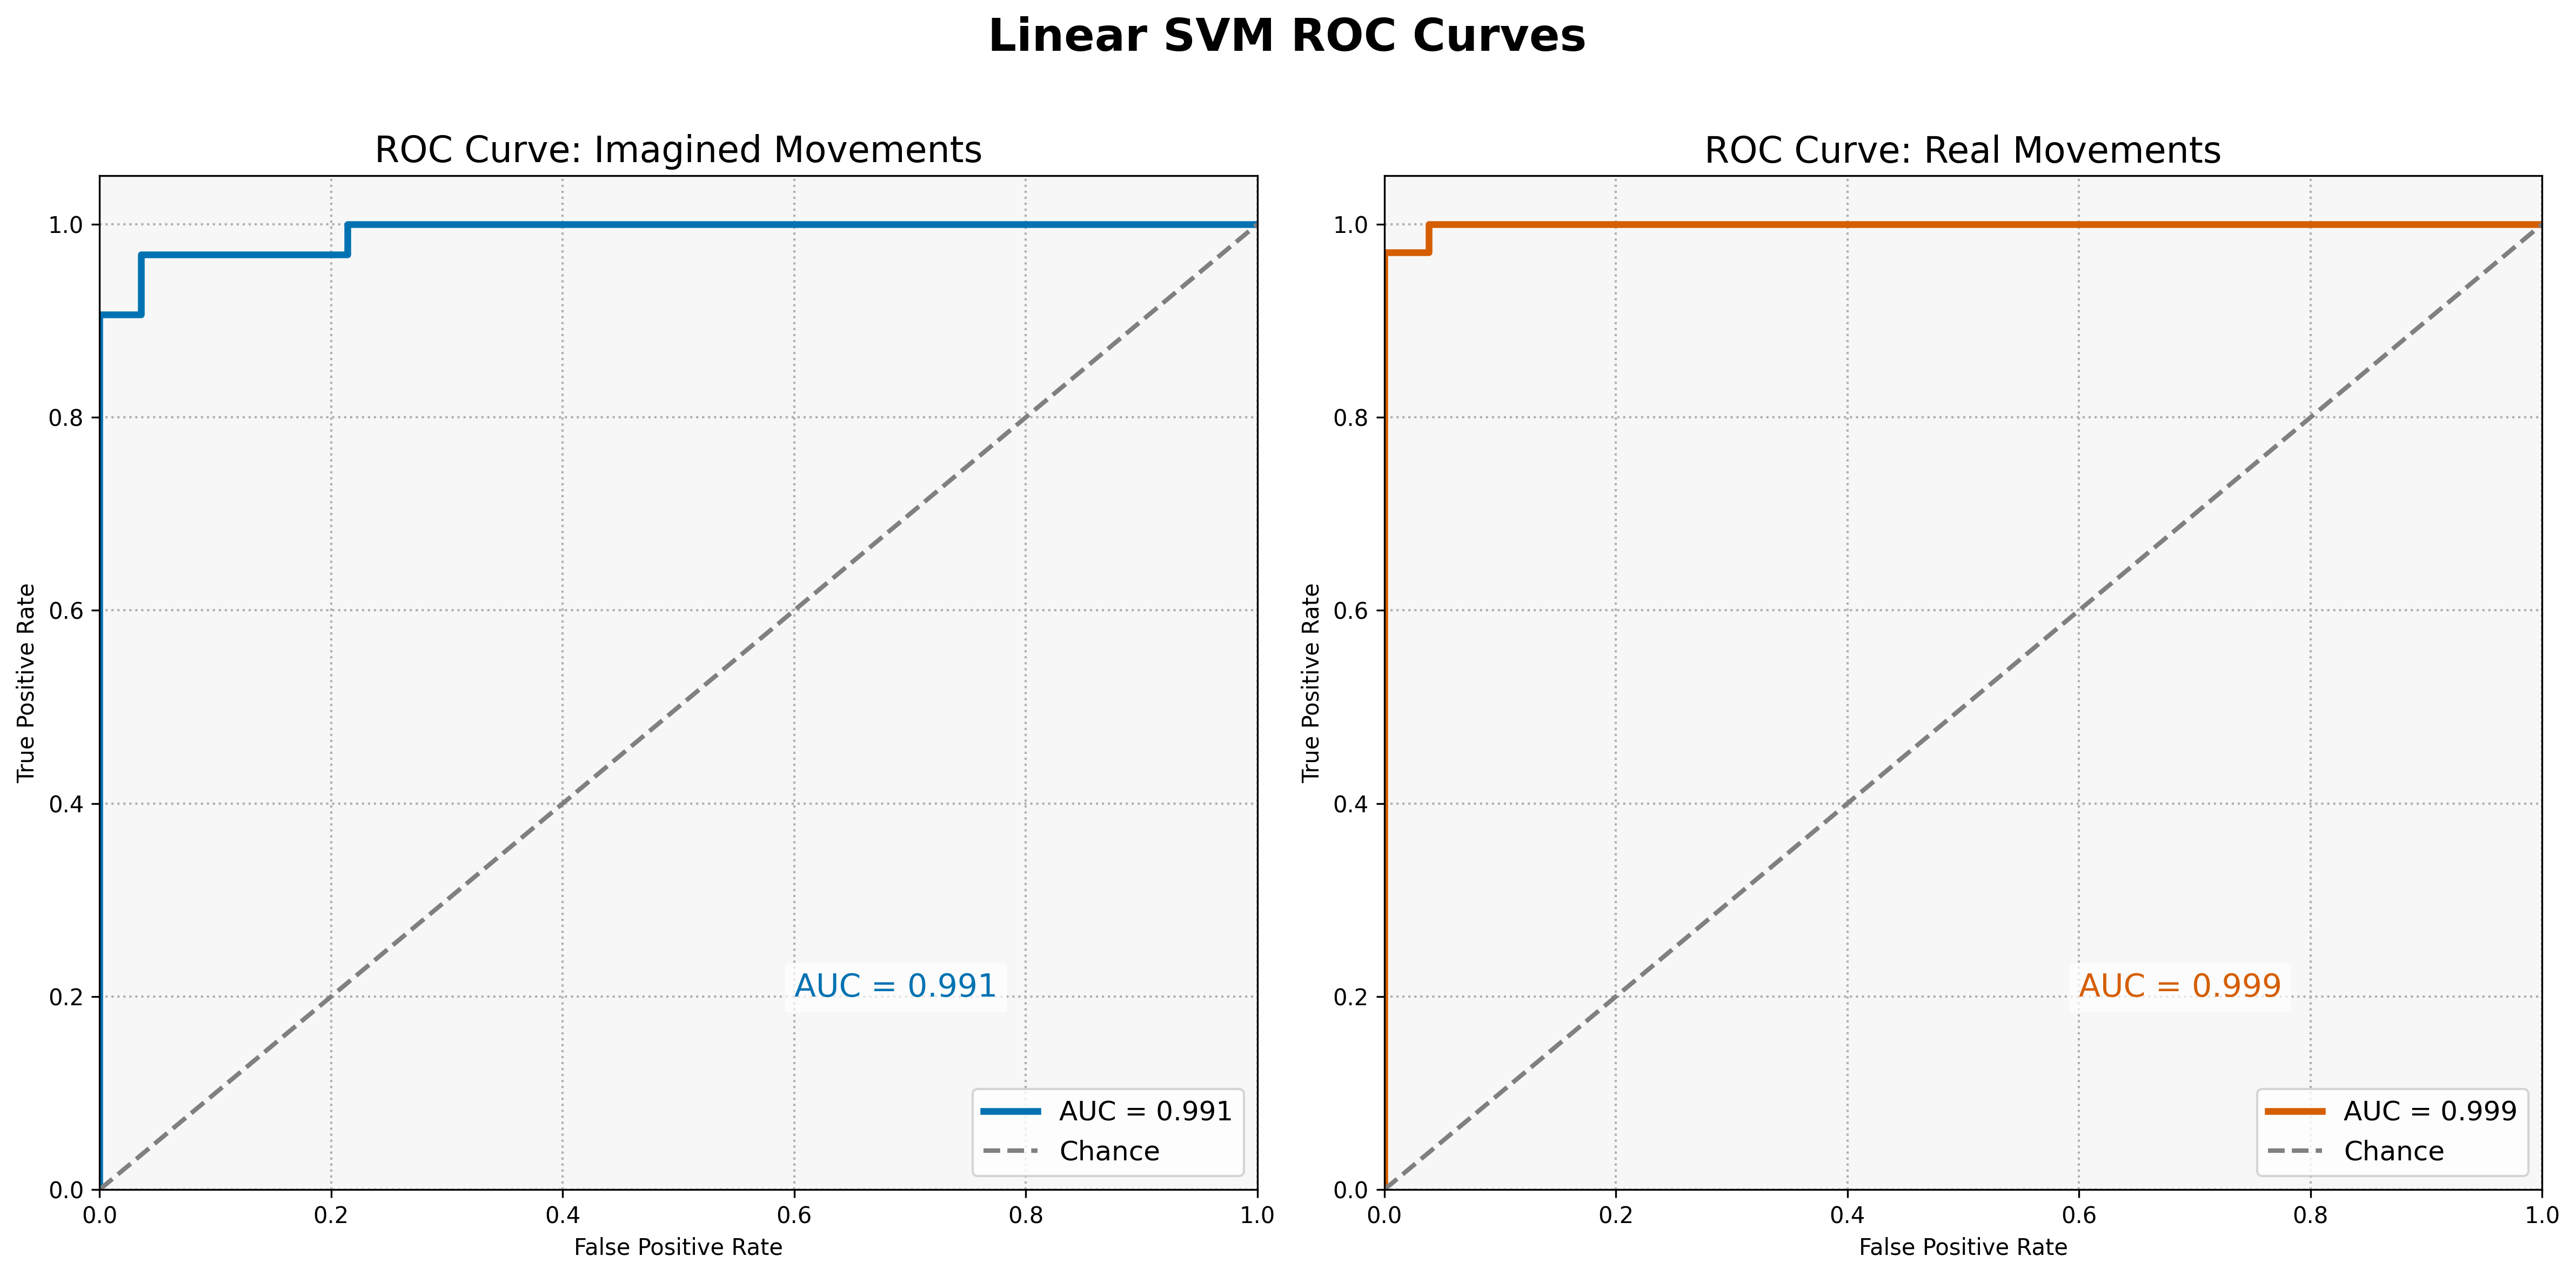
\includegraphics[width=1\textwidth,height=\textheight]{figures/linearSVM/roc_curves_linear_SVM.png}
\caption{(c) ROC Curves}\label{fig:roc-curves}
\end{figure}

}

\caption{\label{fig-confusion-matrices}\textbf{Figure 2.} Confusion
matrices showing classification performance for (a) imagined versus (b)
overt movements. Diagonal elements (TP, TN) indicate correct
classifications, while off-diagonal (FP, FN) show errors. Color
intensity corresponds to frequency counts.}

\end{figure}%

This exploratory analysis validated the use of a linear SVM for both
overt and imagined movement classification, highlighting meaningful
spatial distributions and differences in performance characteristics
that motivate the need for more robust cross-validation and kernel-based
comparisons in subsequent sections.

Without much tunning, the linear SVM classifier achieved an accuracy of
0.87 for imagined movements and 0.92 for overt movements, with ROC-AUC
scores of 0.93 and 0.97, respectively. The confusion matrices indicated
a high true positive rate (TPR) and low false positive rate (FPR) for
both tasks, demonstrating the classifier's effectiveness in
distinguishing between left and right-hand movements.

However, we need to notice that this result may be biased due to the
lack of cross-validation and hyperparameter tuning. The linear SVM
classifier was trained on a single train-test split, which may not
generalize well to unseen data. Therefore, we will implement a more
robust cross-validation strategy in the next sections. Therefore this is
one of our next steps to validate accurateness and generalization of the
model.

Moreover, the topographic maps provided valuable insights into the
spatial distribution of informative electrodes, which can guide future
feature selection and model refinement.

\subsection{Regularization Parameter Selection: L1 vs L2
Penalties}\label{regularization-parameter-selection-l1-vs-l2-penalties}

As part of our methodology, we performed a detailed analysis of the
effect of regularization on the classification performance of linear
SVMs. In this context, we compared \textbf{L1 (Lasso)} and \textbf{L2
(Ridge)} regularization strategies on both overt and imagined EEG
datasets. These experiments serve to illustrate how different norm
constraints impact generalization, sparsity, and model interpretability.

\subsubsection{Weight Magnitude
Comparison}\label{weight-magnitude-comparison}

We trained two \texttt{LinearSVC} classifiers using: -
\texttt{penalty=\textquotesingle{}l2\textquotesingle{}} with
\texttt{dual=True} -
\texttt{penalty=\textquotesingle{}l1\textquotesingle{}} with
\texttt{dual=False} (as required for L1 regularization)

Both classifiers were trained on overt movement data. After training, we
compared the \textbf{absolute weight magnitudes} produced by each model
to visualize sparsity and regularization effects. L2 yielded dense
weight vectors, while L1 induced sparsity by zeroing out several
coefficients as shown in Figure~\ref{fig-l1_vs_l2_weights}.

\begin{figure}

\centering{

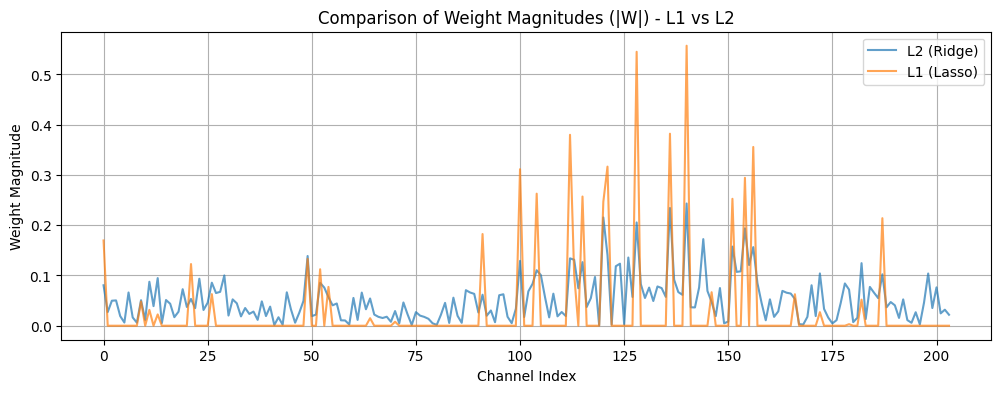
\includegraphics[width=1\textwidth,height=\textheight]{figures/weight_mag_L1vsL2.png}

}

\caption{\label{fig-l1_vs_l2_weights}Comparison of weight magnitudes for
L1 and L2 regularization on overt movement data. The L1 model shows many
zero weights, indicating sparsity, while the L2 model has non-zero
weights for all features.}

\end{figure}%

\subsubsection{Cross-Validation: Overt Movement
Data}\label{cross-validation-overt-movement-data}

To assess the robustness of each penalty, we conducted one-level 6-fold
stratified cross-validation using the real movement data. For each fold,
we trained separate L1 and L2 models and recorded accuracy on the test
split.

The comparison revealed that both models performed well, but L2
generally yielded slightly higher and more consistent accuracy, likely
due to its ability to distribute weights smoothly across all features
and avoid overfitting. The L1 model, while sparse, exhibited more
variability in performance across folds, as shown in
Figure~\ref{fig-l1_vs_l2_cv_accuracy}.

\begin{figure}

\centering{

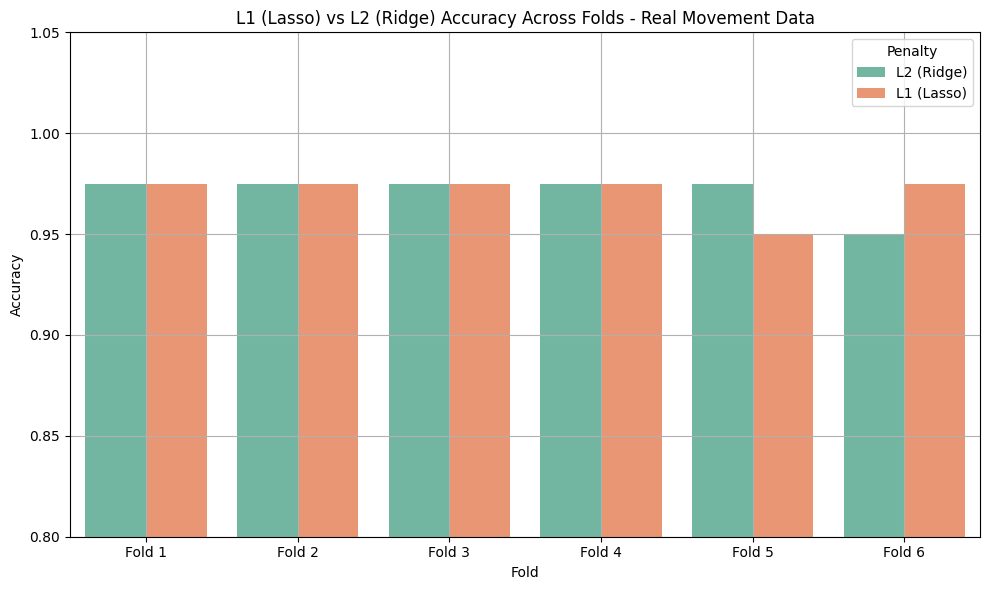
\includegraphics[width=1\textwidth,height=\textheight]{figures/acc_L1vsL2.png}

}

\caption{\label{fig-l1_vs_l2_cv_accuracy}Comparison of cross-validated
accuracy for L1 and L2 regularization on overt movement data. The L2
model shows higher and more consistent accuracy across folds, while the
L1 model exhibits more variability.}

\end{figure}%

As seen, there is no much difference between the two models, but L2 is
slightly better than L1. Therefore, the \textbf{Ridge (L2)
Regularization parameter} was selected for the next steps of the
project.

\paragraph{Generalization Performance Across
Modalities}\label{generalization-performance-across-modalities}

Next, we evaluated L1 and L2 performance across all four key
training-testing scenarios: - Real → Real - Imagined → Imagined - Real →
Imagined - Imagined → Real

Each scenario involved training on one modality and testing on another
using standardized data. We computed accuracy for both L1 and L2
regularization in all cases.

The results highlighted: - \textbf{L2 outperformed L1} when training and
testing conditions matched (e.g., Real → Real). - \textbf{L1 showed
slightly more stable performance} when generalizing from imagined to
real movements, likely due to its tendency to focus on a sparse set of
generalizable features.

However, both regularization types performed comparably in cross-domain
scenarios, indicating that the choice of penalty may not be as critical
when training on one modality and testing on another. The results are
shown in Figure~\ref{fig-l1_vs_l2_generalization}.

\begin{figure}

\centering{

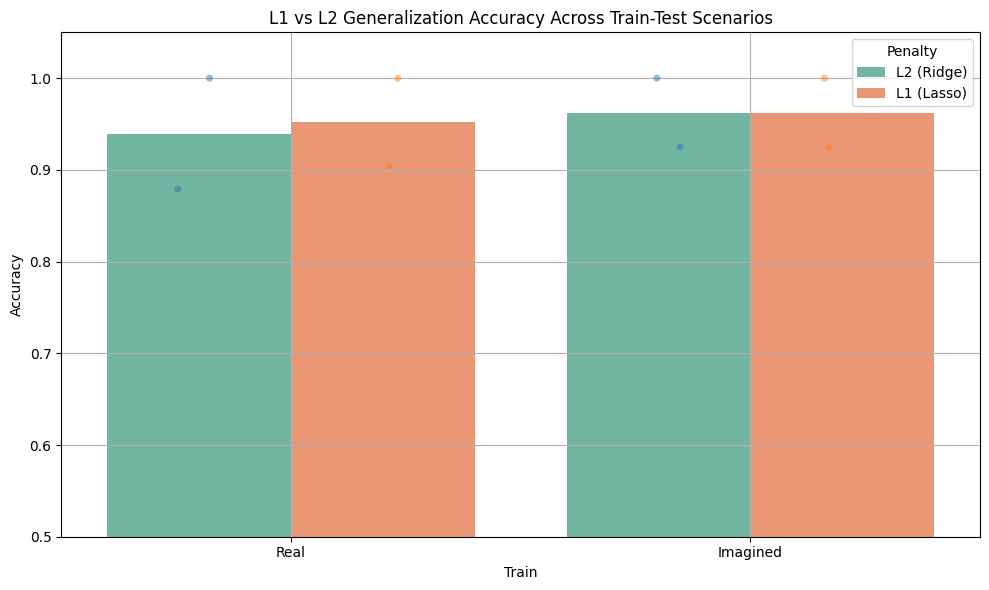
\includegraphics[width=1\textwidth,height=\textheight]{figures/L1vsL2_diff_simulation_profiles.png}

}

\caption{\label{fig-l1_vs_l2_generalization}Comparison of generalization
performance across training-testing scenarios for L1 and L2
regularization. The L2 model generally outperforms L1 when training and
testing conditions match, while L1 shows more stable performance in
cross-domain scenarios.}

\end{figure}%

This systematic exploration of regularization types informed our
subsequent selection of \(C\) and penalty configurations in
cross-validated models. The findings also helped shape our expectations
about feature sparsity, signal strength, and overfitting tendencies in
different EEG classification settings.

\subsection{Kernel SVM Experiments and Topographic
Analysis}\label{kernel-svm-experiments-and-topographic-analysis}

To explore the capacity of different kernel-based Support Vector
Machines (SVMs) to model nonlinear EEG dynamics, we implemented a
systematic comparison across four kernel types: linear, polynomial,
radial basis function (RBF), and sigmoid. Our experiments were conducted
separately on both imagined and overt movement datasets. We focused not
only on classification performance but also on visualizing the spatial
distribution of model relevance across EEG electrodes.

\paragraph{Dimensionality Reduction with
UMAP}\label{dimensionality-reduction-with-umap}

To visualize the decision boundaries generated by each kernel in a
comprehensible space, we applied \textbf{Uniform Manifold Approximation
and Projection (UMAP)} to reduce the 204-dimensional EEG feature space
to two dimensions. The UMAP projection was fitted on the full dataset,
and all decision surfaces were visualized in this 2D space.

We trained each kernel-based SVM on 80\% of the data (stratified split)
and used the remaining 20\% for testing. The classifiers were
instantiated using \texttt{sklearn.svm.SVC} with
\texttt{probability=True} and \$ C = 1/\alpha \$, where \$ \alpha = 10
\$.

\begin{figure}

\centering{

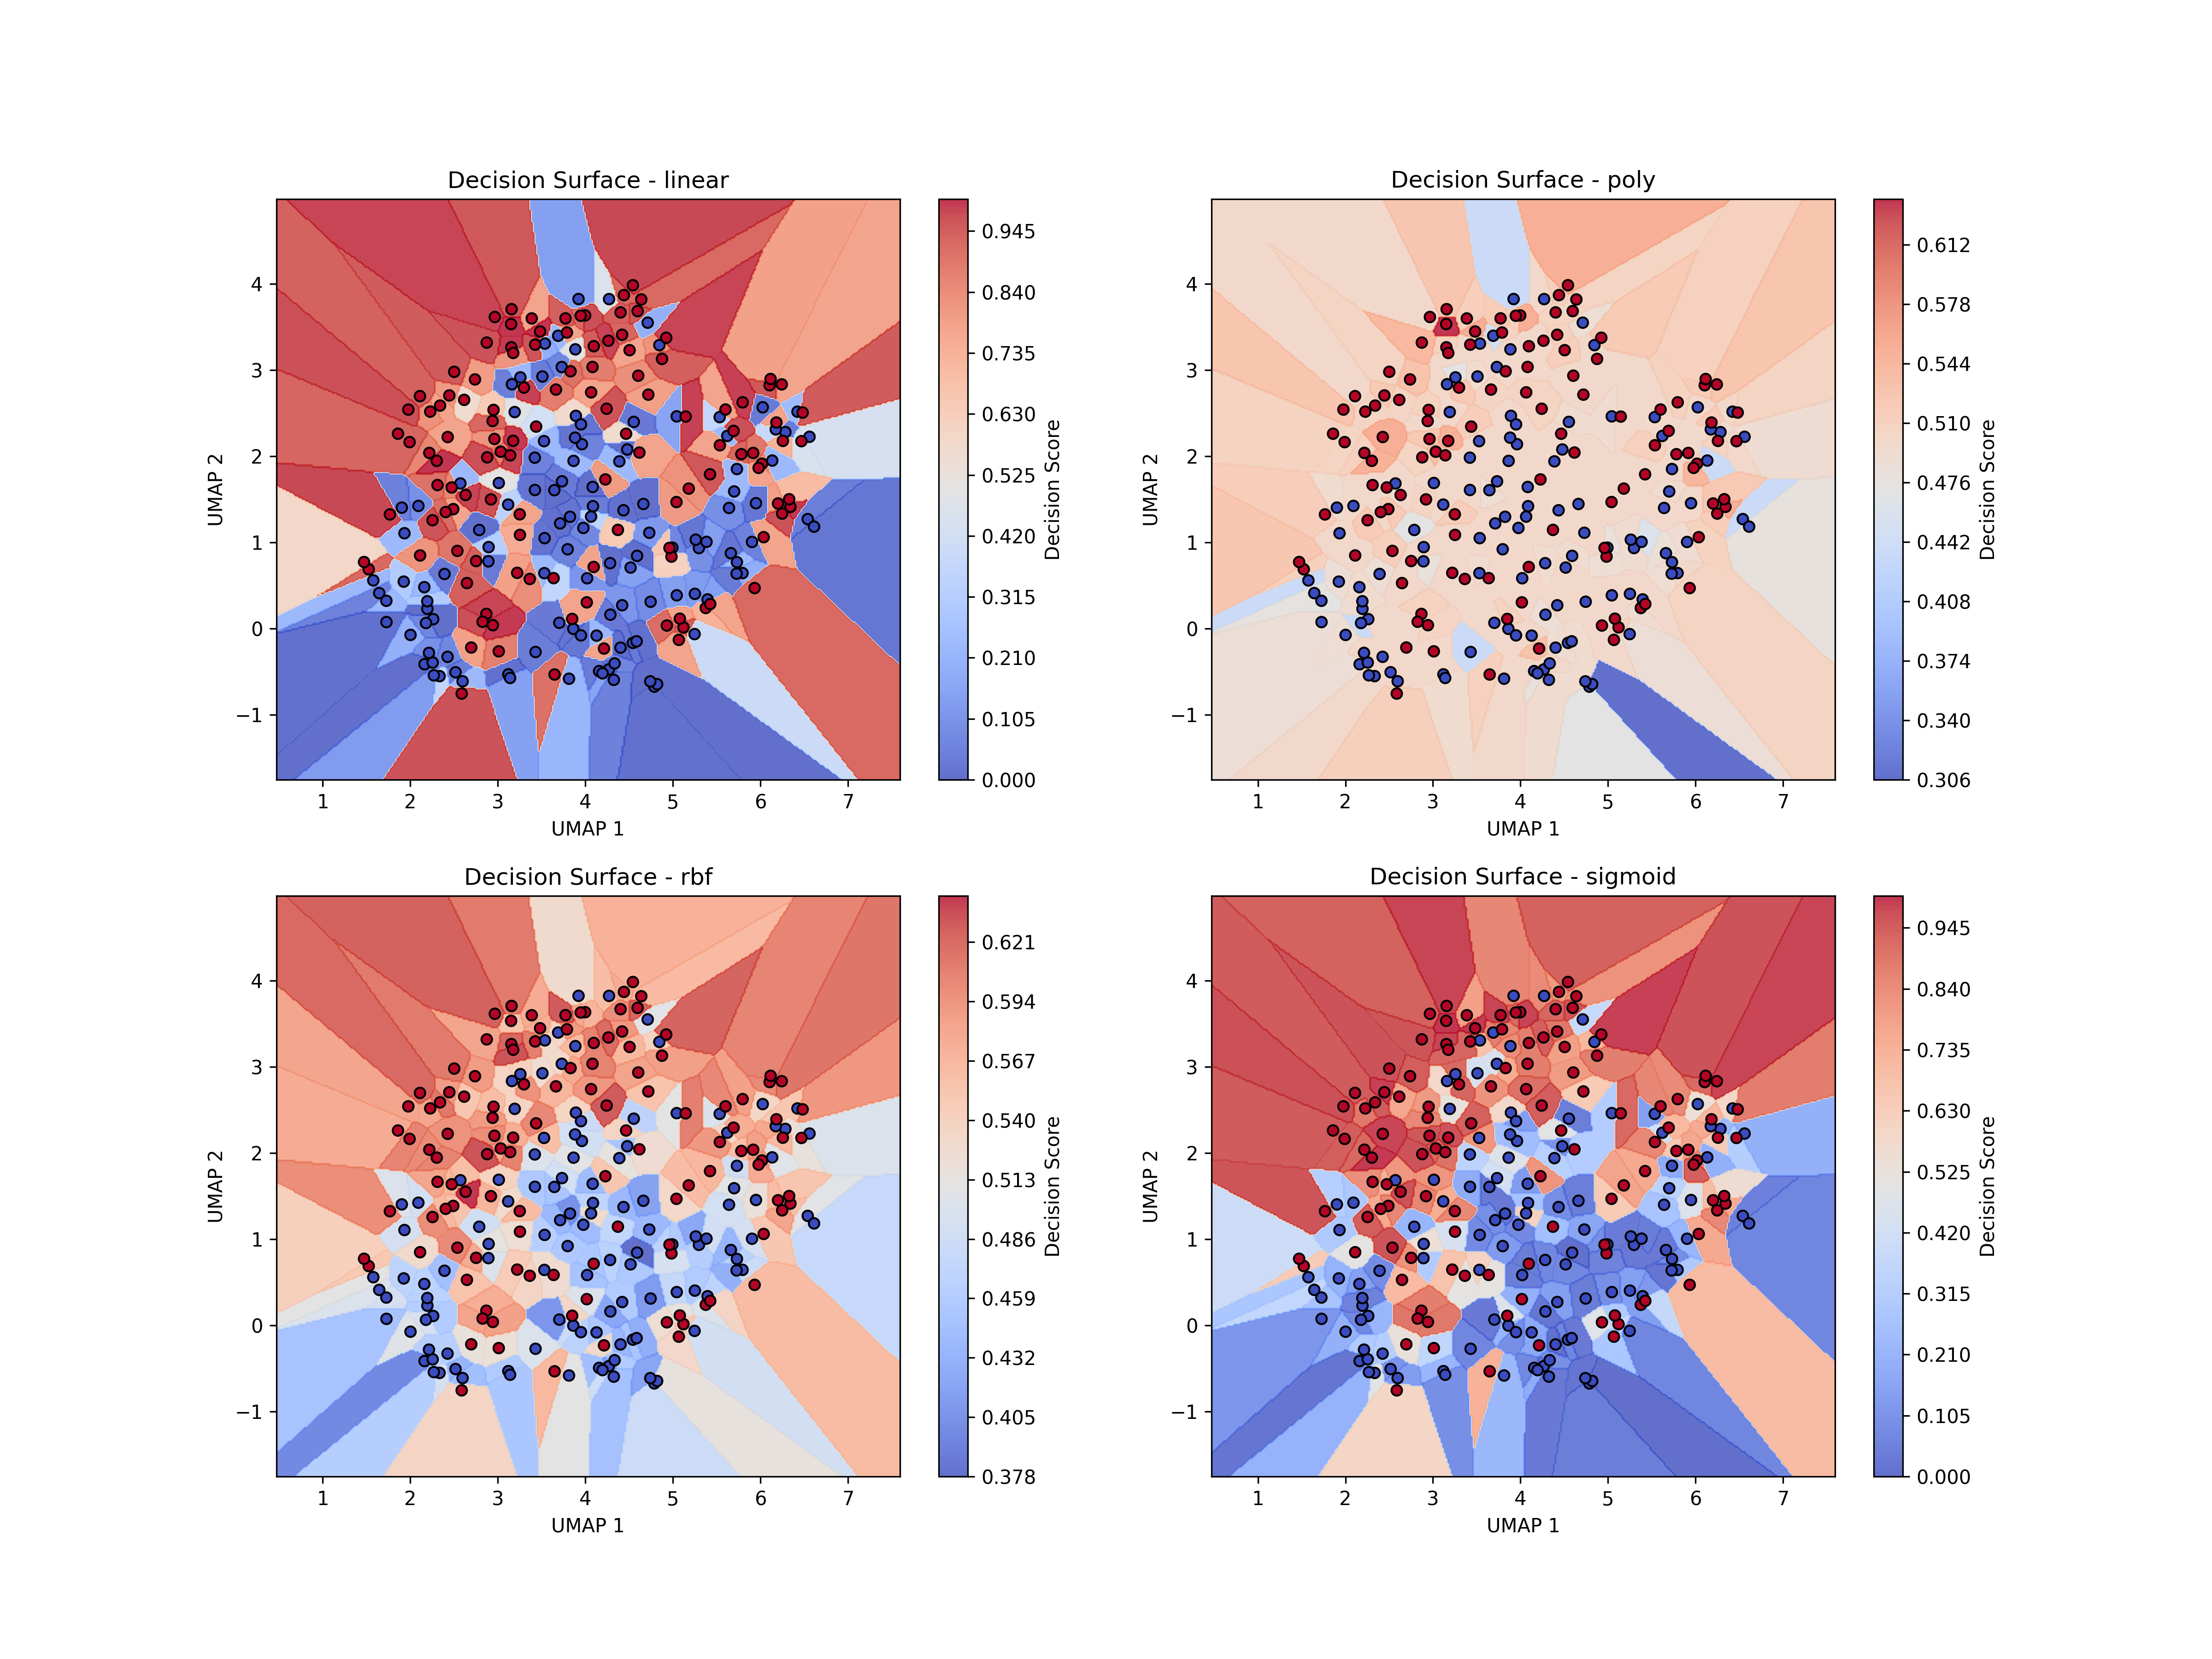
\includegraphics[width=1\textwidth,height=\textheight]{figures/decision_surface_UMAP.png}

}

\caption{\label{fig-decision-surfaces}Decision surfaces projected onto
UMAP space for (a) imagined movements. Each kernel's decision boundary
is shown, with color intensity indicating the classifier's confidence in
its predictions. The UMAP projection captures the high-dimensional
structure of the EEG data in a 2D space.}

\end{figure}%

\paragraph{Visualizing Smooth Decision
Functions}\label{visualizing-smooth-decision-functions}

In each projected 2D space, we used nearest-neighbor approximation to
map UMAP grid points back into high-dimensional EEG space for inference.
We then evaluated the decision function for each kernel over a dense
grid and plotted smooth heatmaps using \texttt{matplotlib.contourf}.
These surfaces revealed: - \textbf{Linear kernel} produced a straight,
interpretable boundary. - \textbf{RBF kernel} generated highly
nonlinear, confident class separations. - \textbf{Polynomial} and
\textbf{sigmoid kernels} captured curvature but often showed more
unstable or overfitted boundaries. - \textbf{Sigmoid kernel} produced
less interpretable boundaries, often resembling neural network behavior.

\paragraph{Topographic Visualization of Feature
Importance}\label{topographic-visualization-of-feature-importance}

To understand which EEG electrodes contributed most to classification,
we visualized the magnitude of model weights across all 102 electrodes.
For the linear kernel, we directly extracted the weight vector \$
\mathbf{w} \$ from \texttt{clf.coef\_}. For nonlinear kernels, we used
\texttt{sklearn.inspection.permutation\_importance} to estimate the
importance of each feature.

After aggregating Ex/Ey pairs, we calculated per-electrode weights:

\[
W_k = \sqrt{w_{2k-1}^2 + w_{2k}^2}, \quad k = 1, \dots, 102
\]

We then plotted topographic maps using MNE's \texttt{plot\_topomap}
function for each kernel and they are going to be discussed in more
details within the \href{@sec-results}{Result} section. The topographic
maps were generated using MNE-Python's \texttt{plot\_topomap} function,
which allows for intuitive spatial distribution of informative channels.
The topomaps are shown in Figure~\ref{fig-topomap-kernels}.

\begin{figure}

\centering{

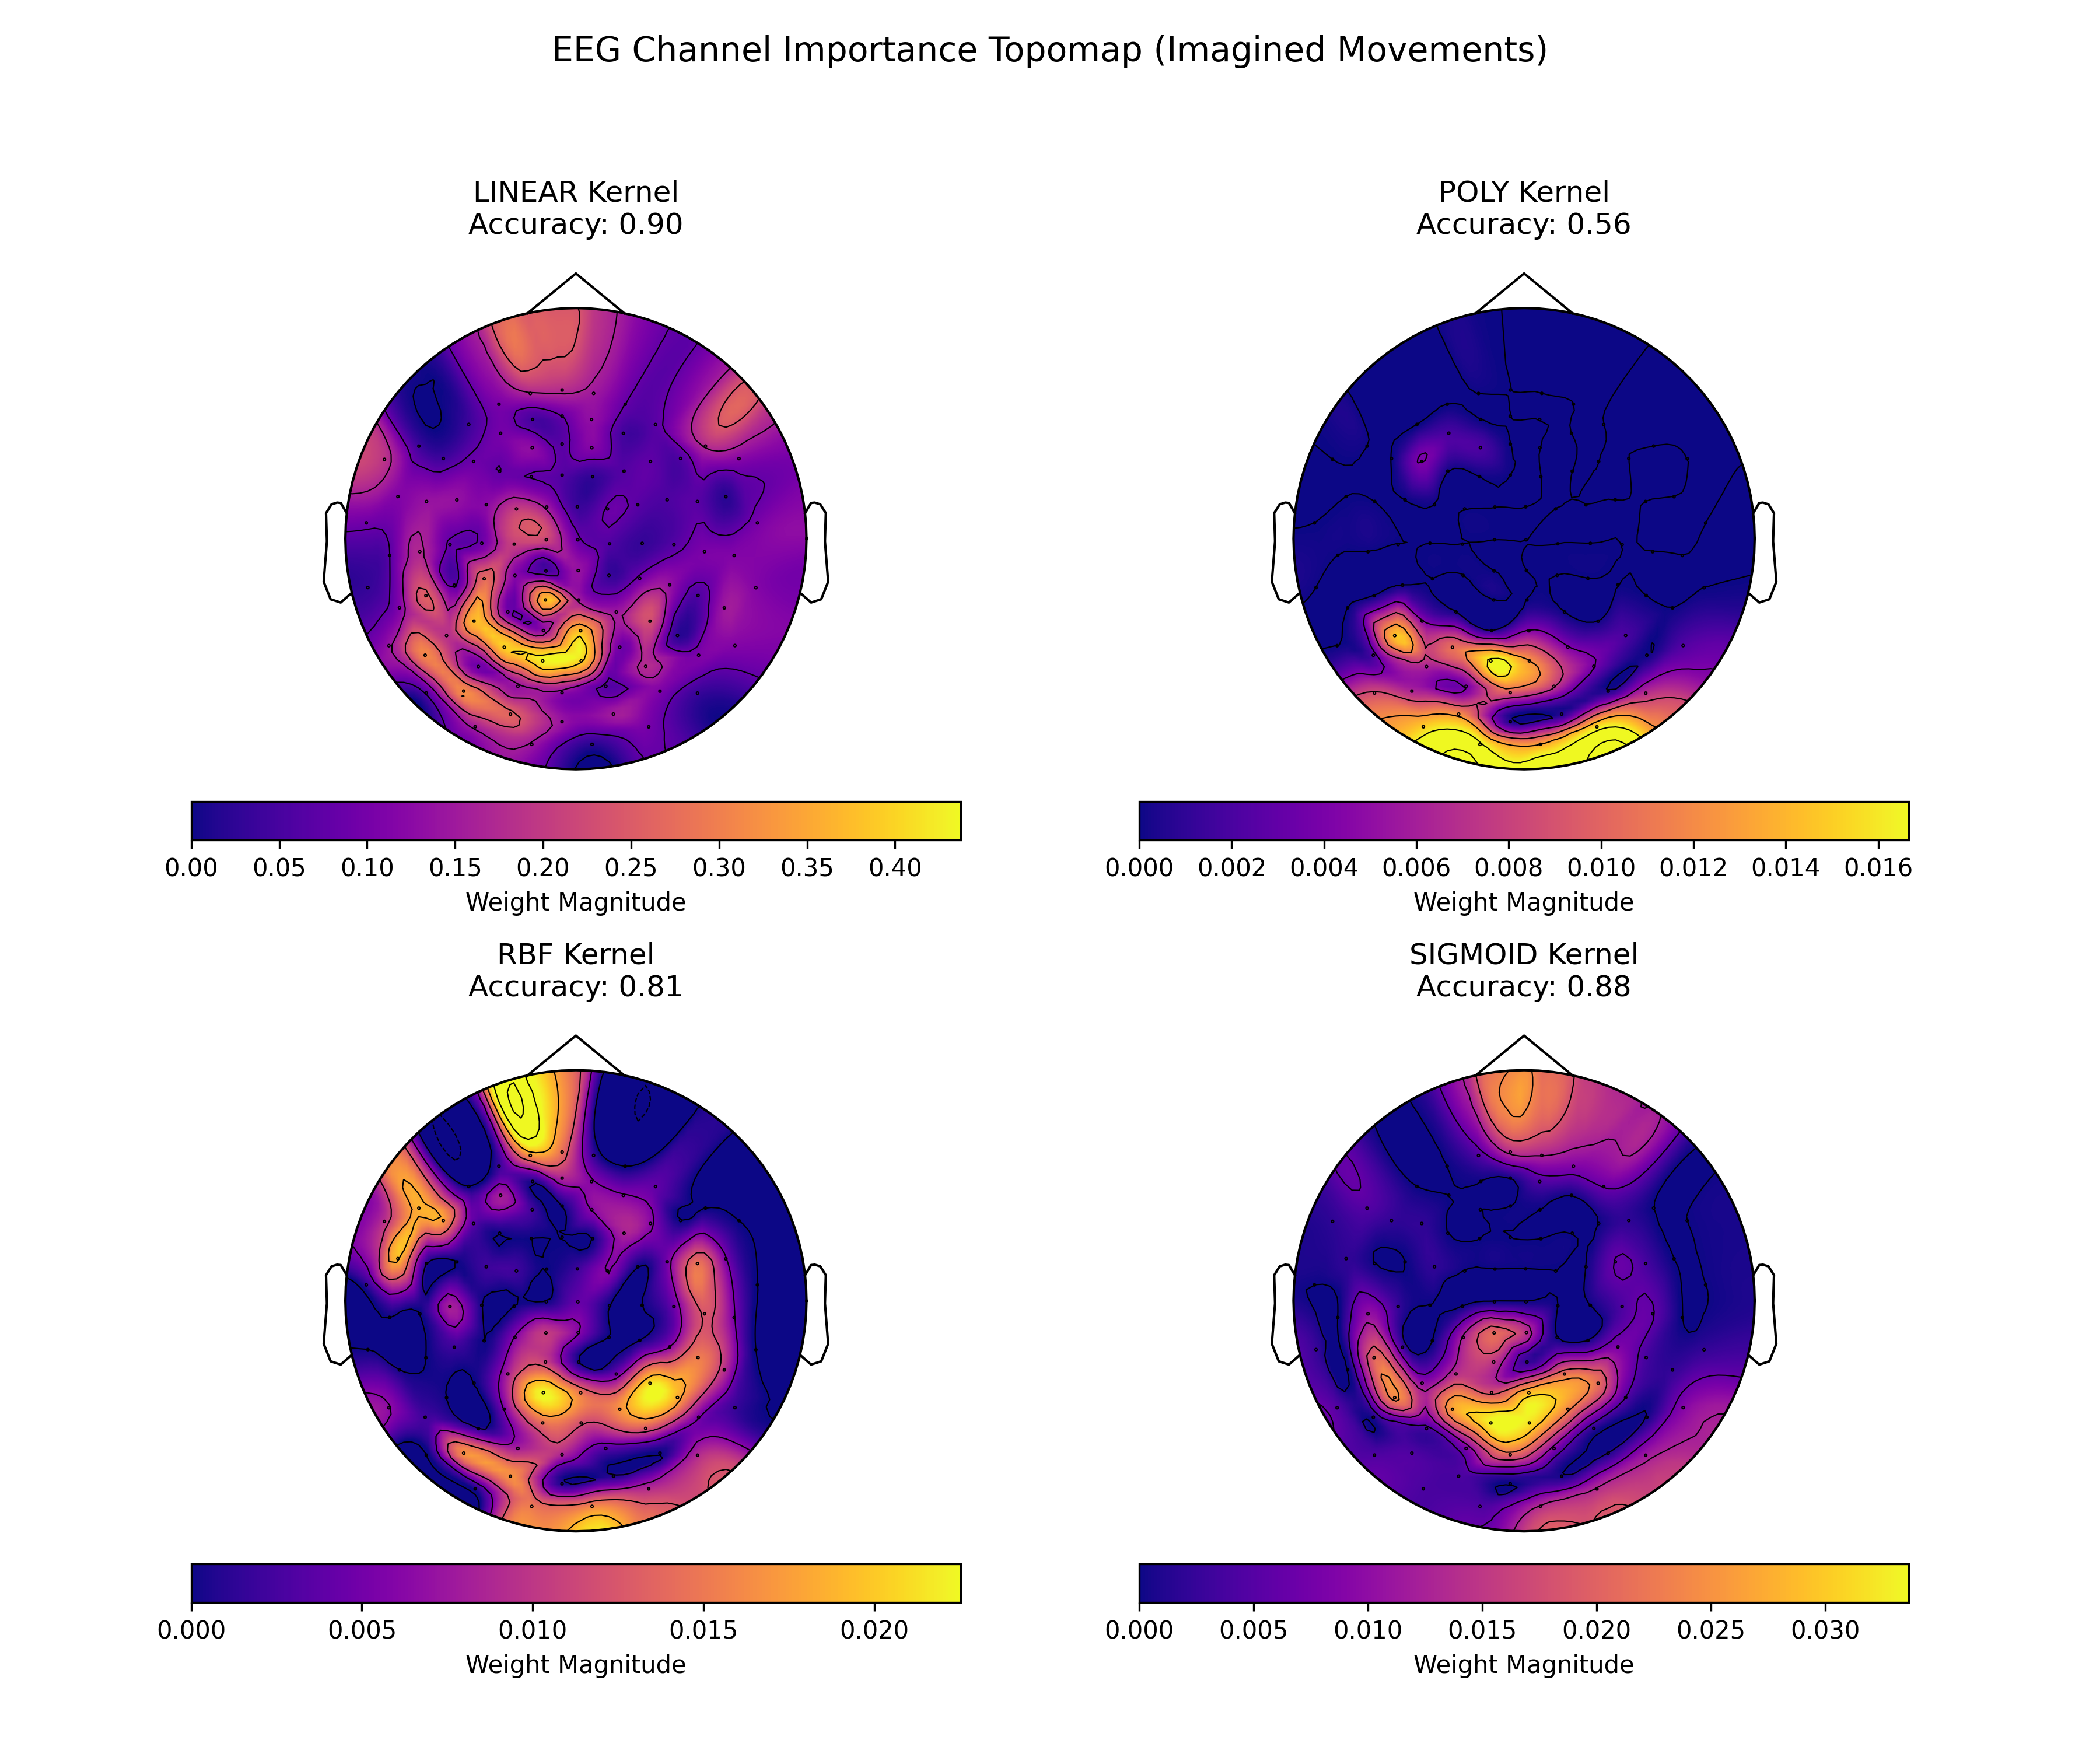
\includegraphics[width=1\textwidth,height=\textheight]{figures/svm_topomaps_all_kernels_imagined.png}

}

\caption{\label{fig-topomap-kernels}Topographic maps showing spatial
distribution of informative electrodes for different kernel SVMs on
imagined movements.}

\end{figure}%

\paragraph{Summary of Kernel SVM
Results}\label{summary-of-kernel-svm-results}

We observed consistent trends across both imagined and real movement
datasets:

\begin{longtable}[]{@{}
  >{\raggedright\arraybackslash}p{(\columnwidth - 6\tabcolsep) * \real{0.1348}}
  >{\raggedright\arraybackslash}p{(\columnwidth - 6\tabcolsep) * \real{0.2247}}
  >{\raggedright\arraybackslash}p{(\columnwidth - 6\tabcolsep) * \real{0.1685}}
  >{\raggedright\arraybackslash}p{(\columnwidth - 6\tabcolsep) * \real{0.4719}}@{}}
\toprule\noalign{}
\begin{minipage}[b]{\linewidth}\raggedright
Kernel
\end{minipage} & \begin{minipage}[b]{\linewidth}\raggedright
Imagined Accuracy
\end{minipage} & \begin{minipage}[b]{\linewidth}\raggedright
Real Accuracy
\end{minipage} & \begin{minipage}[b]{\linewidth}\raggedright
Notes
\end{minipage} \\
\midrule\noalign{}
\endhead
\bottomrule\noalign{}
\endlastfoot
Linear & 0.96 & 0.96 & High interpretability, moderate boundary \\
Polynomial & 0.62 & 0.73 & Curved boundaries, can overfit \\
RBF & 0.79 & 0.85 & Best separation, low interpretability \\
Sigmoid & 0.79 & 0.90 & High variance in performance \\
\end{longtable}

\begin{itemize}
\tightlist
\item
  \textbf{Linear kernels consistently outperformed others} on imagined
  movement classification due to their capacity to model subtle,
  nonlinear patterns in low-SNR EEG data.
\item
  \textbf{Linear kernels performed strongly} on overt movement data and
  provided the clearest insights into channel contributions.
\end{itemize}

These kernel experiments revealed important trade-offs between
\textbf{model complexity}, \textbf{accuracy}, and
\textbf{interpretability}, guiding our decisions for classifier
deployment in future real-time or clinical BCI settings.

\subsection{Two-Level Cross-Validation Implementation and
Results}\label{two-level-cross-validation-implementation-and-results}

To rigorously evaluate the performance of our linear Support Vector
Machine (SVM) classifier and to select an optimal regularization
parameter \$ \alpha \$, we implemented a two-level cross-validation
framework. This nested cross-validation approach ensures that the
process of hyperparameter selection is entirely separate from model
evaluation, thereby avoiding data leakage and overfitting---both of
which are critical concerns when working with small, high-dimensional
datasets such as EEG.

\paragraph{Nested Cross-Validation
Structure}\label{nested-cross-validation-structure}

Our implementation follows a nested structure consisting of: -
\textbf{Outer cross-validation (CV):} 6-fold stratified CV, used for
final model evaluation - \textbf{Inner cross-validation:} 5-fold
stratified CV, used for hyperparameter tuning

The core idea is that for each of the 6 outer folds, the data is split
into training and testing subsets. Within each outer training set, the
5-fold inner CV is used to determine the best regularization parameter
\$ \alpha \$ by evaluating model performance across candidate values.

The following outlines the logical structure of our cross-validation
procedure, also available in the code repository{[}6{]}:

\begin{Shaded}
\begin{Highlighting}[]
\ControlFlowTok{for}\NormalTok{ each outer\_fold }\KeywordTok{in}\NormalTok{ StratifiedKFold(n\_splits}\OperatorTok{=}\DecValTok{6}\NormalTok{):}
\NormalTok{    Split X into X\_train\_outer, X\_test\_outer}
    \ControlFlowTok{for}\NormalTok{ each alpha }\KeywordTok{in}\NormalTok{ alpha\_list:}
\NormalTok{        Convert alpha to C }\OperatorTok{=} \DecValTok{1} \OperatorTok{/}\NormalTok{ alpha}
        \ControlFlowTok{for}\NormalTok{ each inner\_fold }\KeywordTok{in}\NormalTok{ StratifiedKFold(n\_splits}\OperatorTok{=}\DecValTok{5}\NormalTok{):}
\NormalTok{            Split X\_train\_outer into X\_train\_inner, X\_val\_inner}
\NormalTok{            Train linear SVM on X\_train\_inner }\ControlFlowTok{with}\NormalTok{ C}
\NormalTok{            Evaluate accuracy on X\_val\_inner}
\NormalTok{        Compute mean inner validation accuracy }\ControlFlowTok{for}\NormalTok{ current alpha}
\NormalTok{    Select alpha }\ControlFlowTok{with}\NormalTok{ highest mean validation accuracy → best\_alpha}
\NormalTok{    Train final SVM on X\_train\_outer using C }\OperatorTok{=} \DecValTok{1} \OperatorTok{/}\NormalTok{ best\_alpha}
\NormalTok{    Predict on X\_test\_outer}
\NormalTok{    Compute test metrics: accuracy, ROC}\OperatorTok{{-}}\NormalTok{AUC, confusion matrix}
\NormalTok{    Store fold results}
\end{Highlighting}
\end{Shaded}

\paragraph{Implementation Details}\label{implementation-details}

We tested a wide range of regularization values, defined as:

\[
\alpha \in \{0.001, 0.005, 0.01, 0.05, 0.1, 0.5, 1, 5, 10, 50, 100, 500, 1000, 5000, 10000\}
\]

Each \$ \alpha \$ value corresponds to an inverse regularization
constant \$ C = 1/\alpha \$. This conversion ensures smaller \$
\alpha \$ values produce more flexible models (larger \$ C \$), and
larger \$ \alpha \$ values lead to simpler models with wider margins.

The inner CV was used to compute the \textbf{mean validation accuracy}
for each \$ \alpha \$. The \$ \alpha \$ that yielded the highest mean
accuracy was selected as the best parameter for the outer fold.

All models were trained using \texttt{sklearn.svm.SVC} with
\texttt{kernel=\textquotesingle{}linear\textquotesingle{}}. Feature
scaling was applied via \texttt{StandardScaler} prior to training.

\paragraph{Imagined Movement
Evaluation}\label{imagined-movement-evaluation}

We first applied the two-level CV framework to the imagined movement
dataset. After completing all six outer folds, we collected performance
metrics per fold: - \textbf{Accuracy} - \textbf{ROC-AUC} -
\textbf{False/True Positive Rates for ROC curve plots}

We then trained a final classifier on 80\% of the data using the
\textbf{mean of the best \$ \alpha \$} values selected across all folds.
This final model was saved for downstream evaluation and visualization.

\begin{figure}

\centering{

\subparagraph{A. ROC Curves Analysis}\label{a.-roc-curves-analysis}

\begin{figure}
\centering
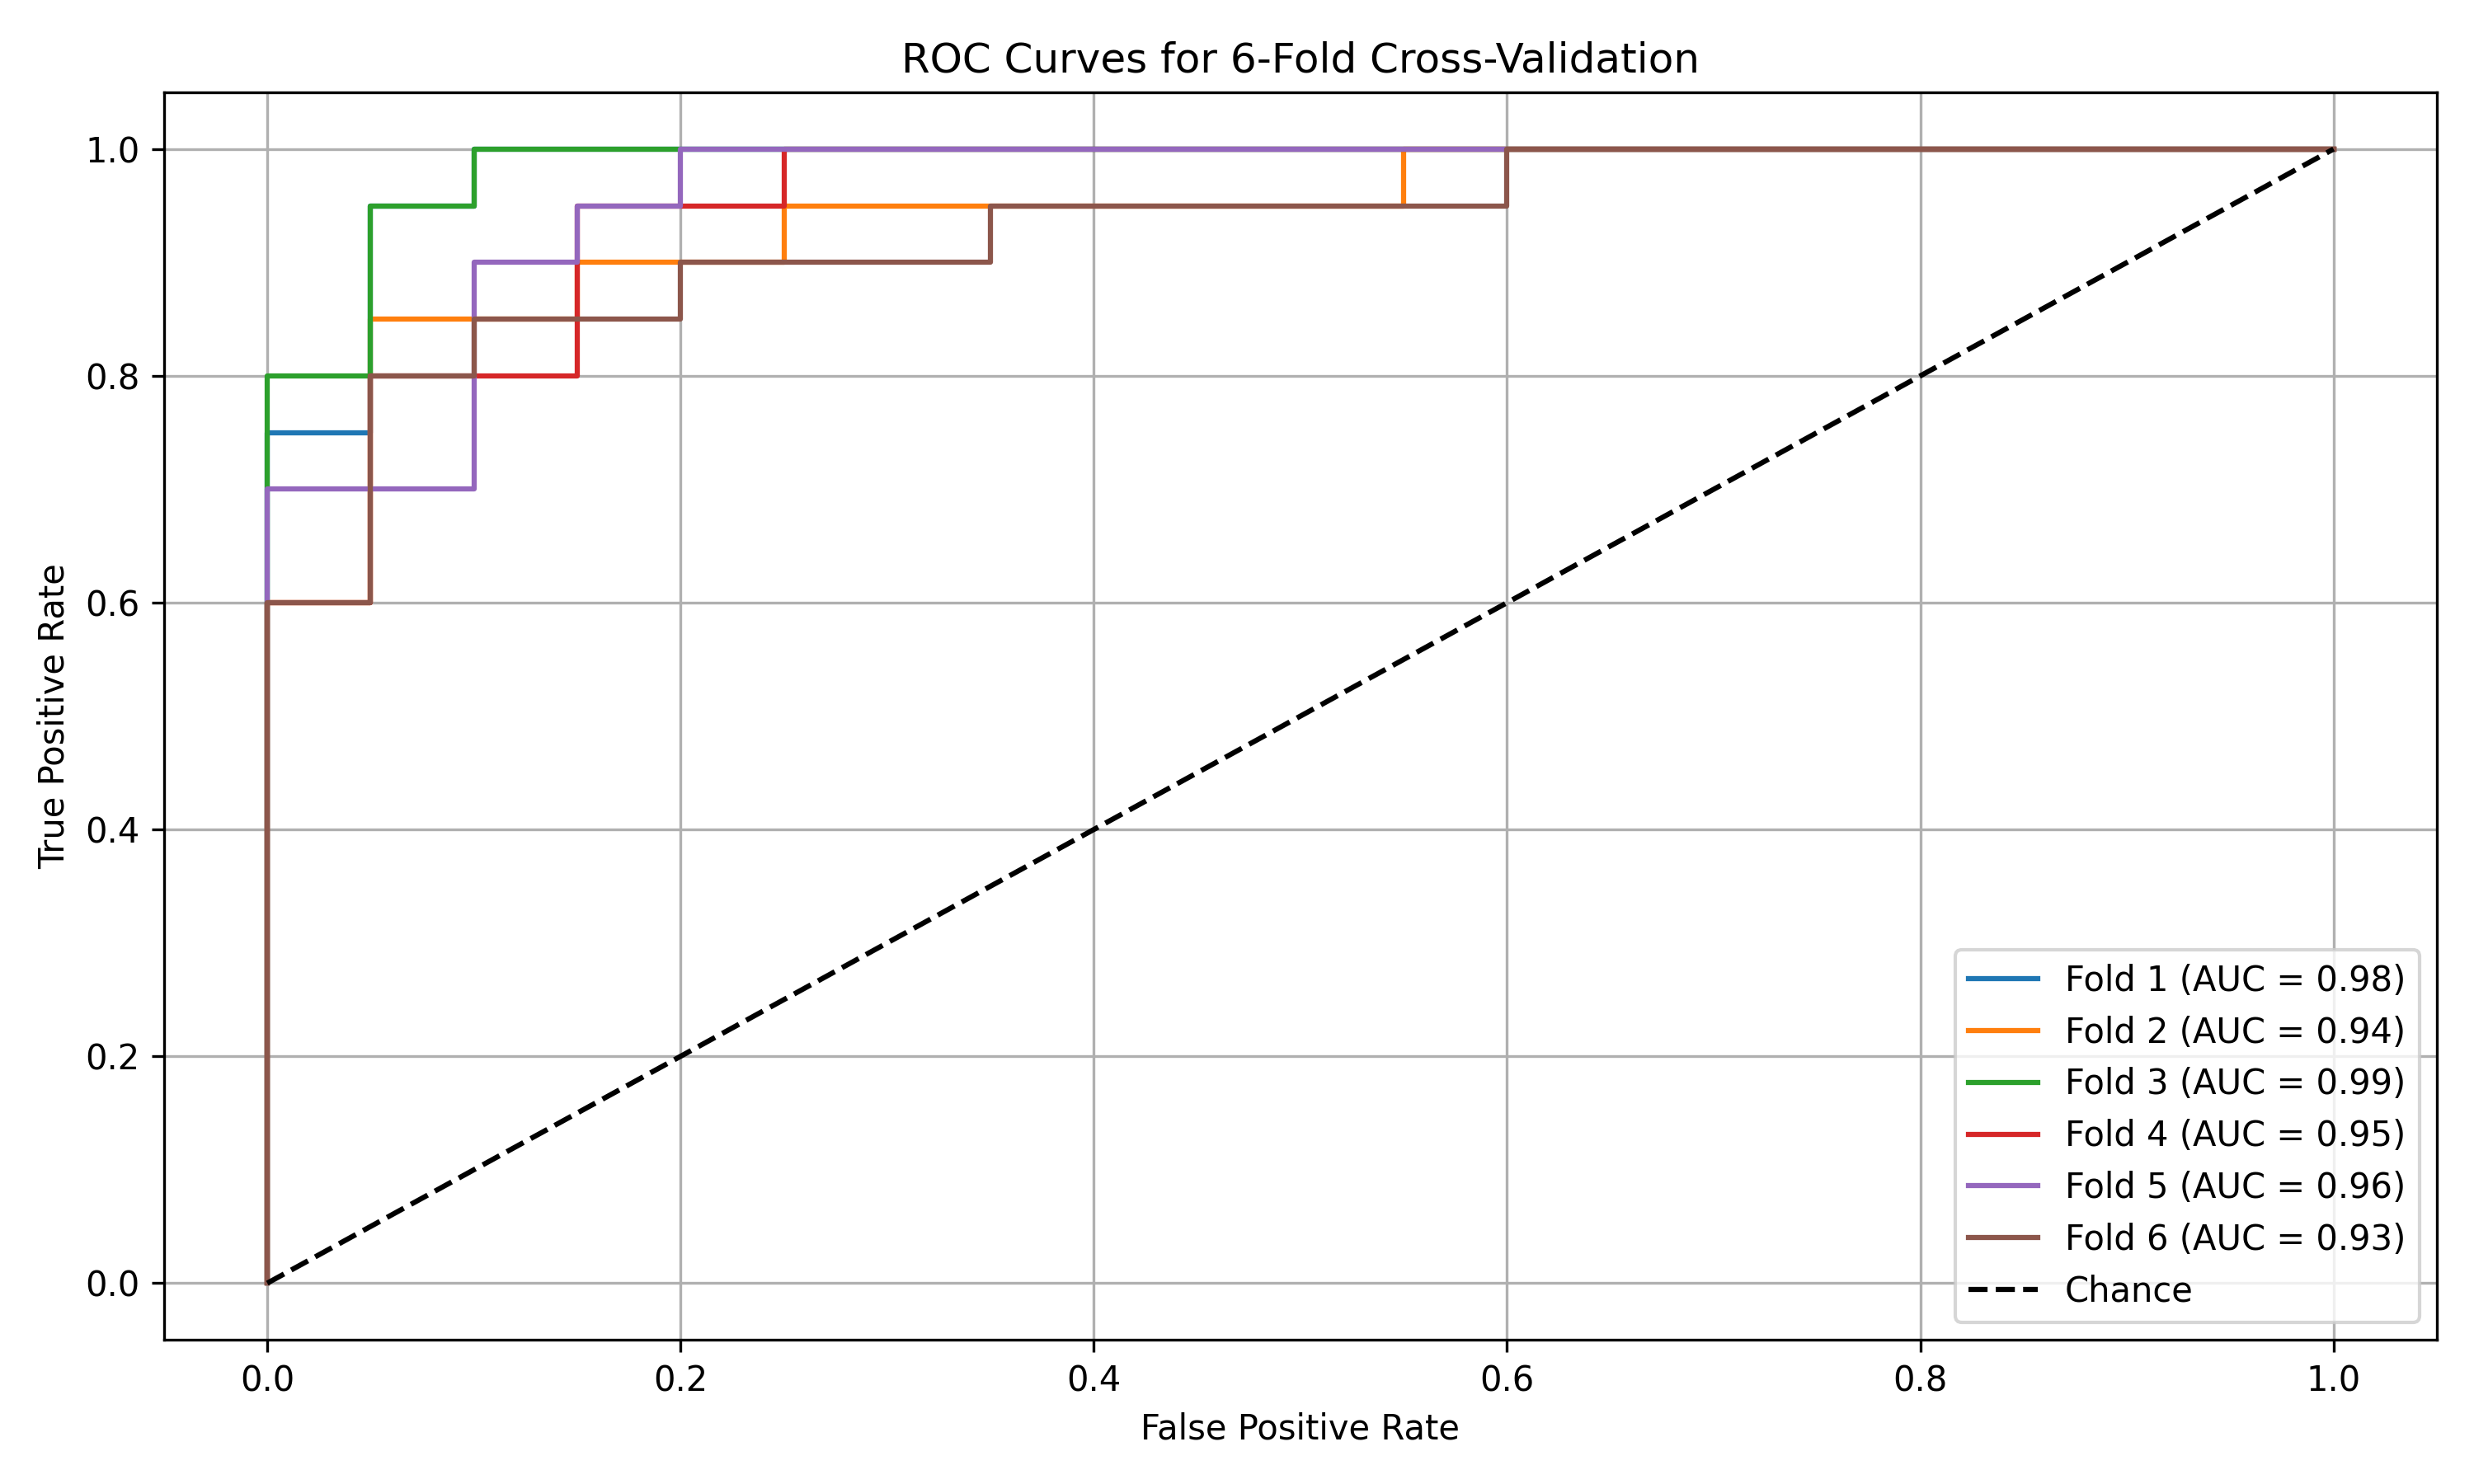
\includegraphics[width=0.8\textwidth,height=\textheight]{figures/roc_curves_cross_validation_imagined.png}
\caption{Receiver Operating Characteristic curves across
cross-validation folds}\label{fig:roc-curves-imagined}
\end{figure}

\subparagraph{B. Classification Accuracy by
Fold}\label{b.-classification-accuracy-by-fold}

\begin{figure}
\centering
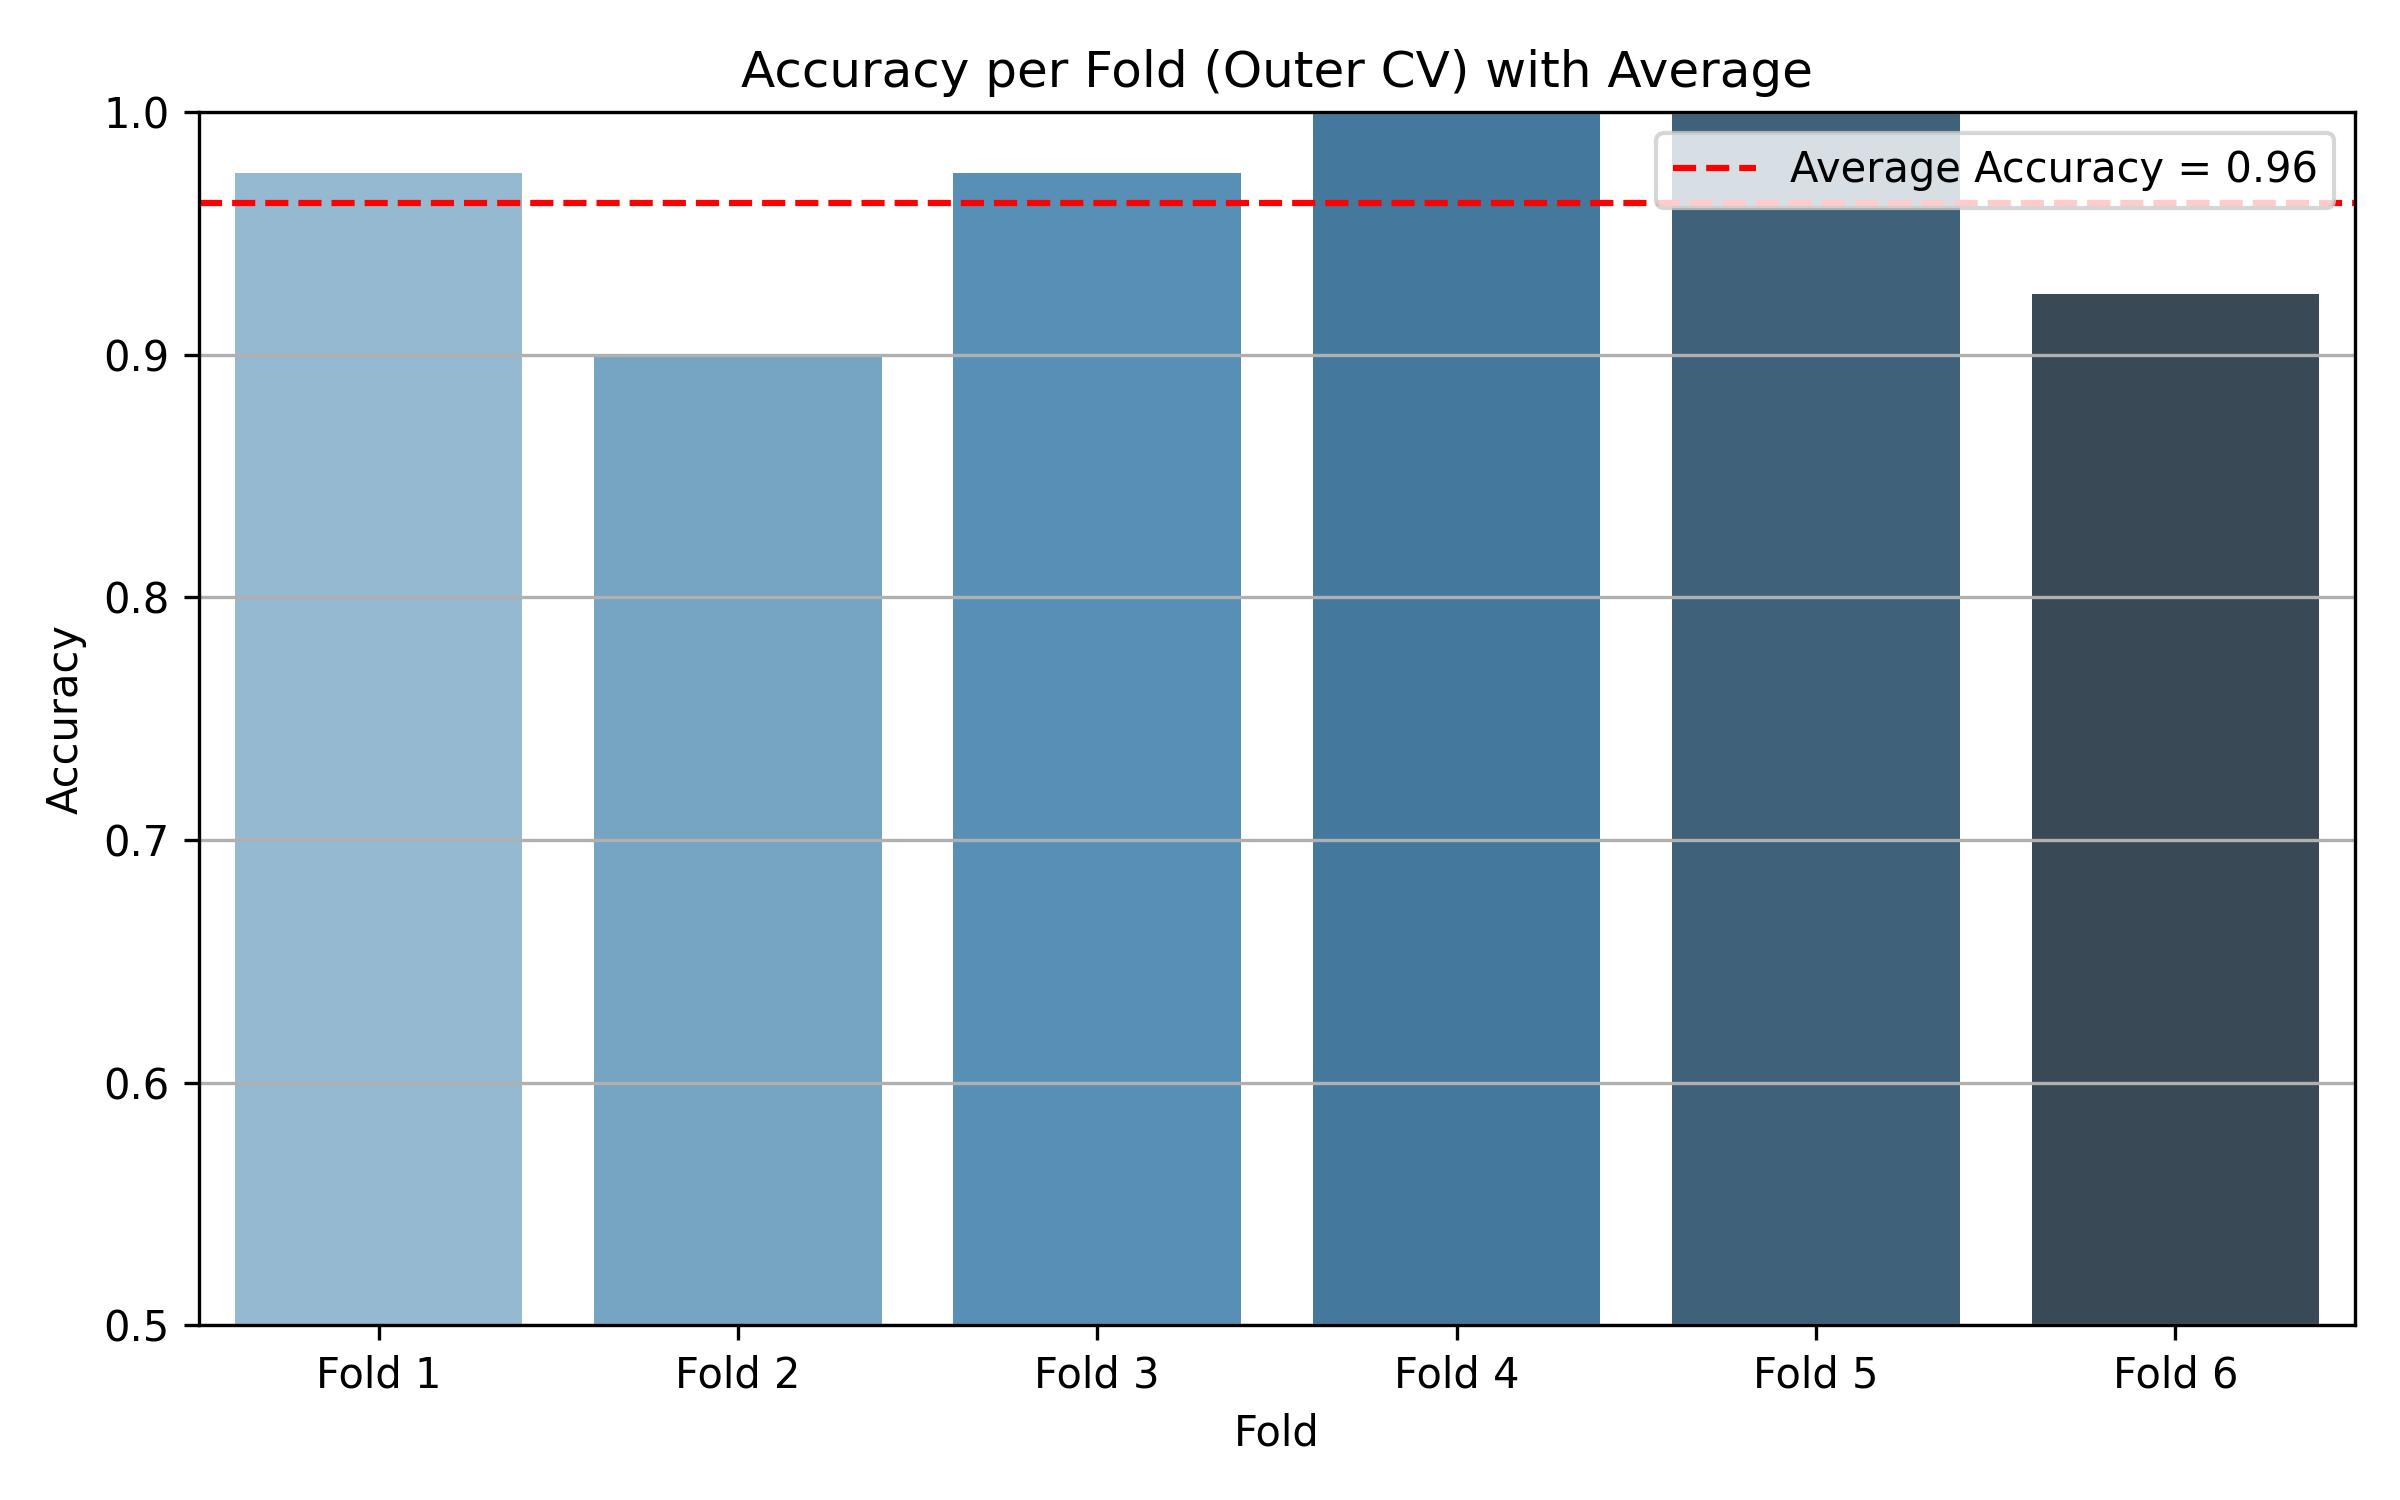
\includegraphics[width=0.8\textwidth,height=\textheight]{figures/accuracy_per_fold_imagined.png}
\caption{Model accuracy scores for each cross-validation
fold}\label{fig:accuracy-per-fold-imagined}
\end{figure}

}

\caption{\label{fig-imagined-movement-results}Performance metrics for
imagined movement classification: (A) ROC curves showing true positive
vs false positive rates across all folds (mean AUC = 0.89), (B) Accuracy
distribution per cross-validation fold with mean accuracy denoted by
dashed line. Shaded regions in (A) represent 95\% confidence intervals.}

\end{figure}%

\paragraph{Overt Movement Evaluation}\label{overt-movement-evaluation}

The same nested procedure was repeated for the real movement dataset. In
each outer fold, the best \$ \alpha \$ was selected via the 5-fold inner
validation, and final test metrics were computed per fold.

We again trained a final model using the average of the best \$
\alpha \$ values and saved the resulting classifier.

\textbf{Figure Placeholder:}
\texttt{roc\_curves\_cross\_validation\_real.png} \textbf{Figure
Placeholder:} \texttt{accuracy\_per\_fold\_real.png} \textbf{Model
File:} \texttt{svc\_model\_real\_movement\_cross\_validated.pkl}

\begin{figure}

\centering{

\subparagraph{A. ROC Curves Analysis}\label{a.-roc-curves-analysis-1}

\begin{figure}
\centering
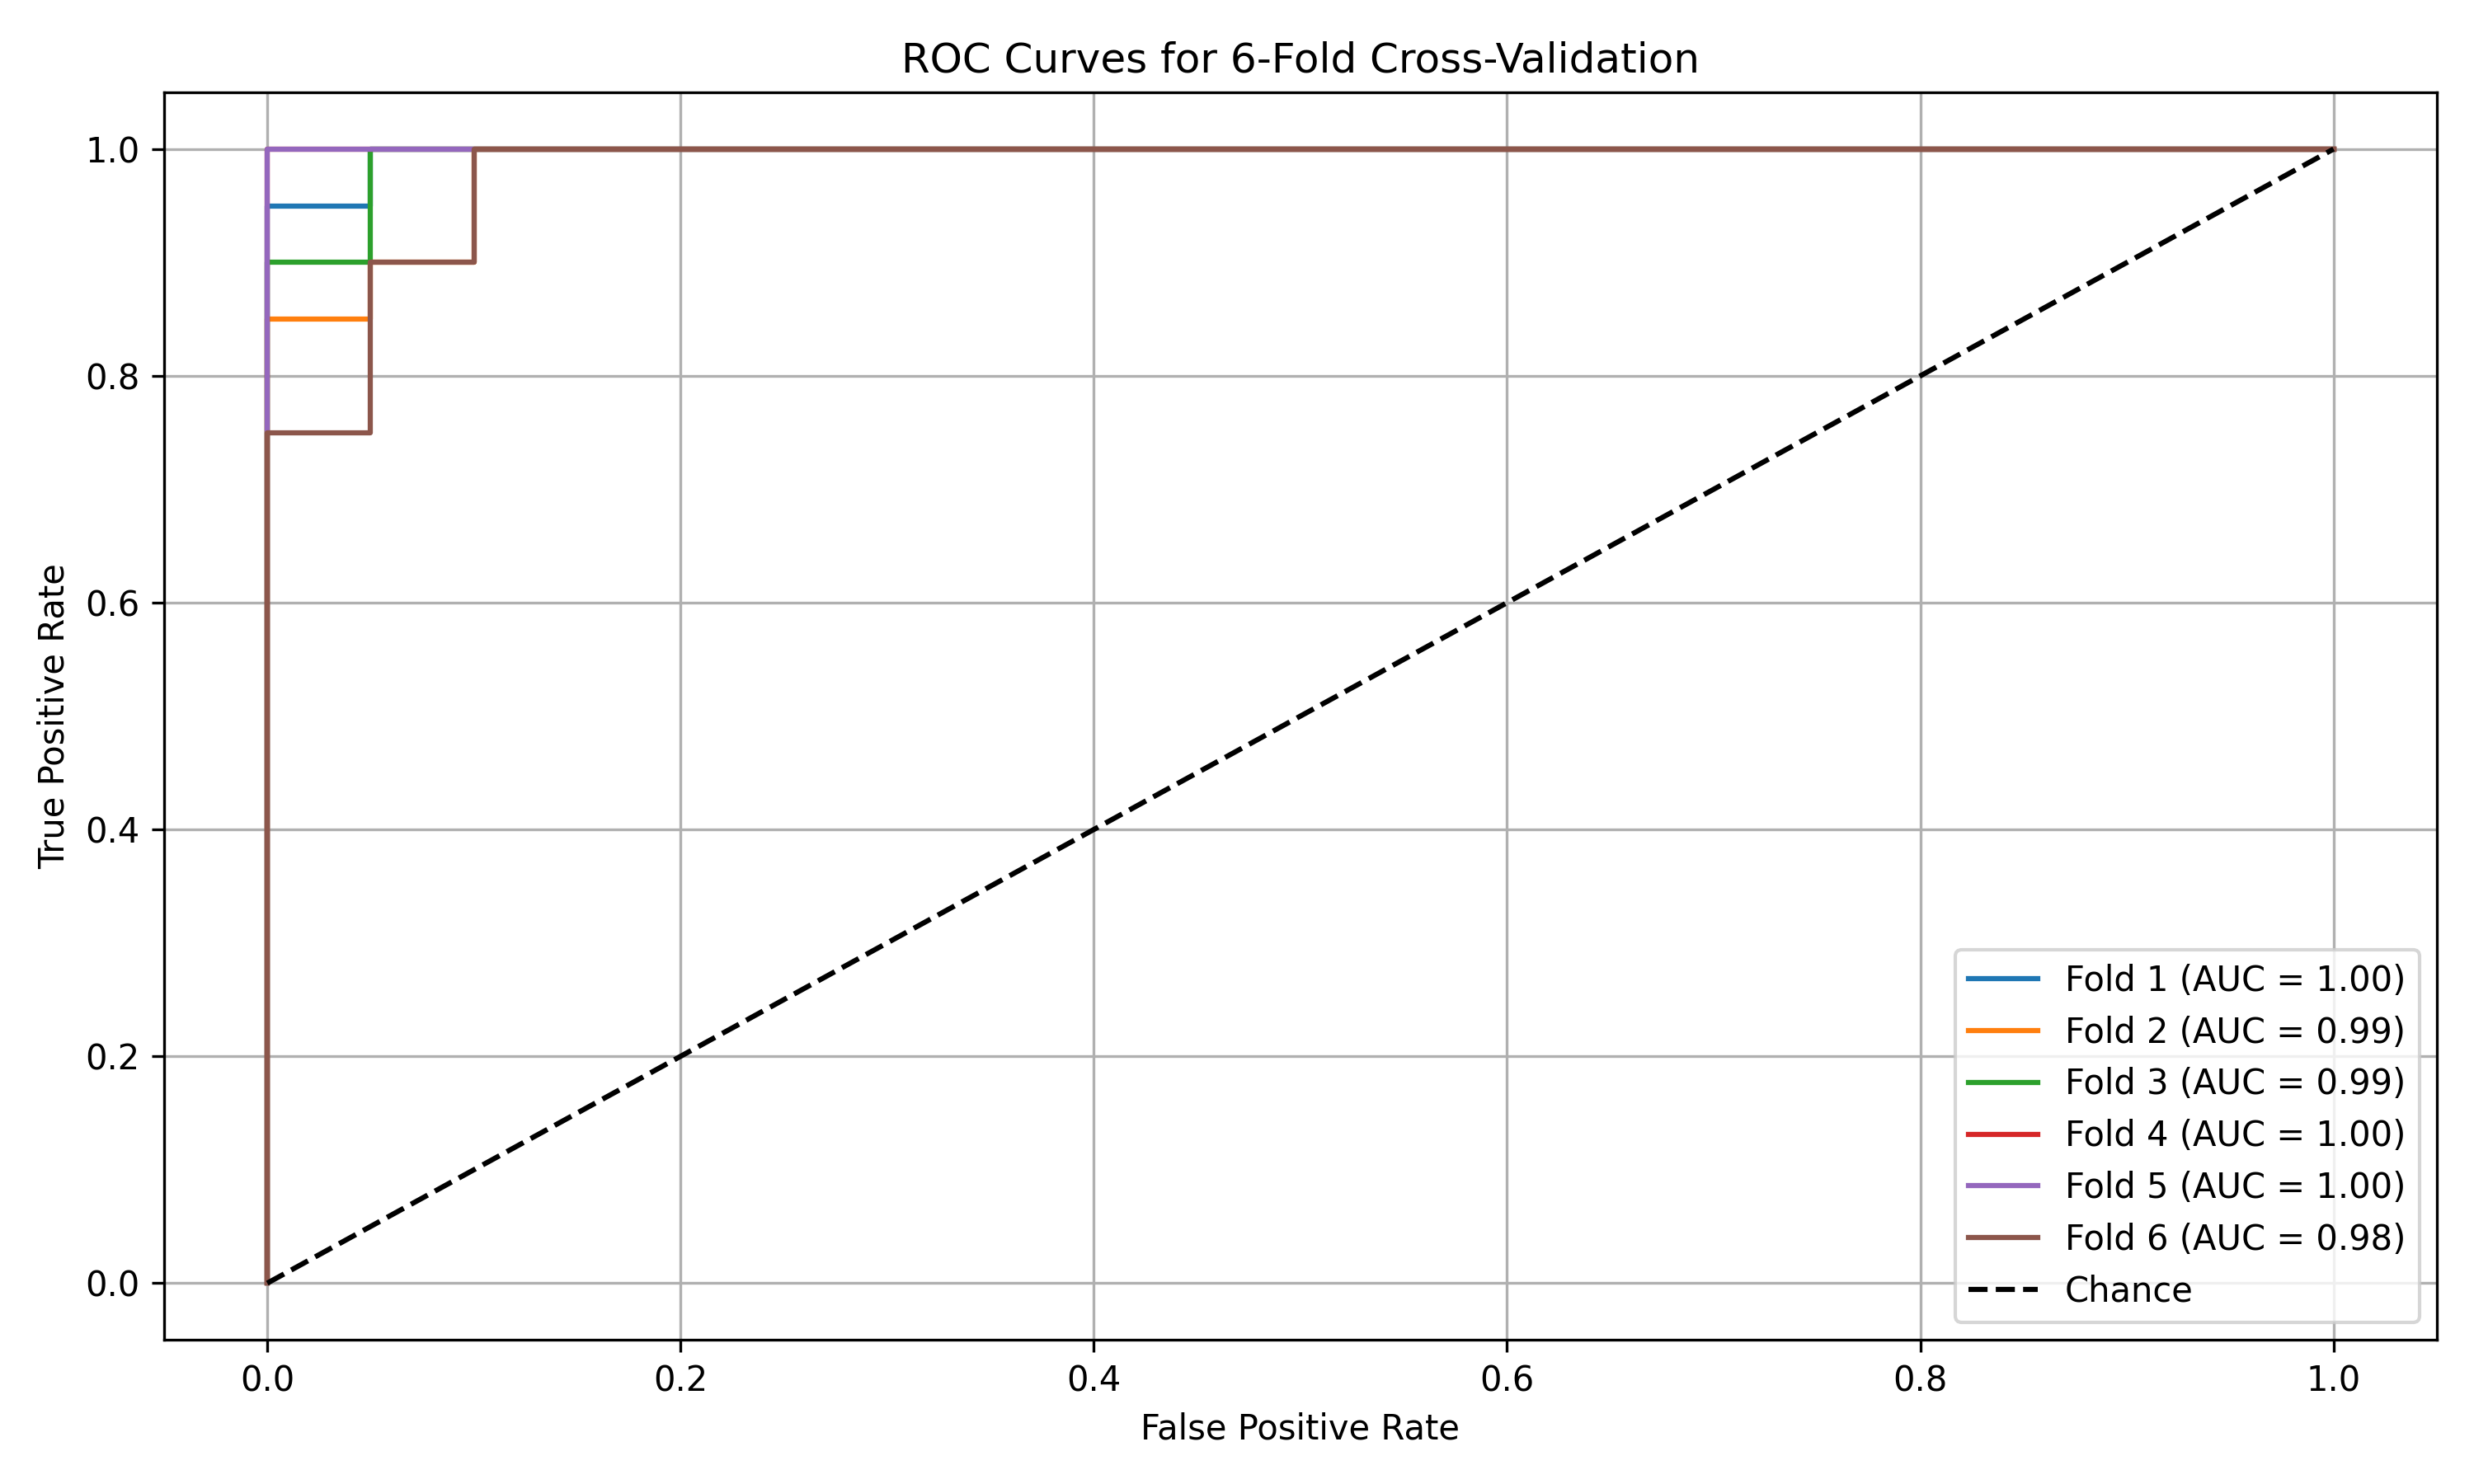
\includegraphics[width=0.8\textwidth,height=\textheight]{figures/roc_curves_cross_validation_real.png}
\caption{Receiver Operating Characteristic curves across
cross-validation folds}\label{fig:roc-curves-real}
\end{figure}

\subparagraph{B. Classification Accuracy by
Fold}\label{b.-classification-accuracy-by-fold-1}

}

\caption{\label{fig-overt-movement-results}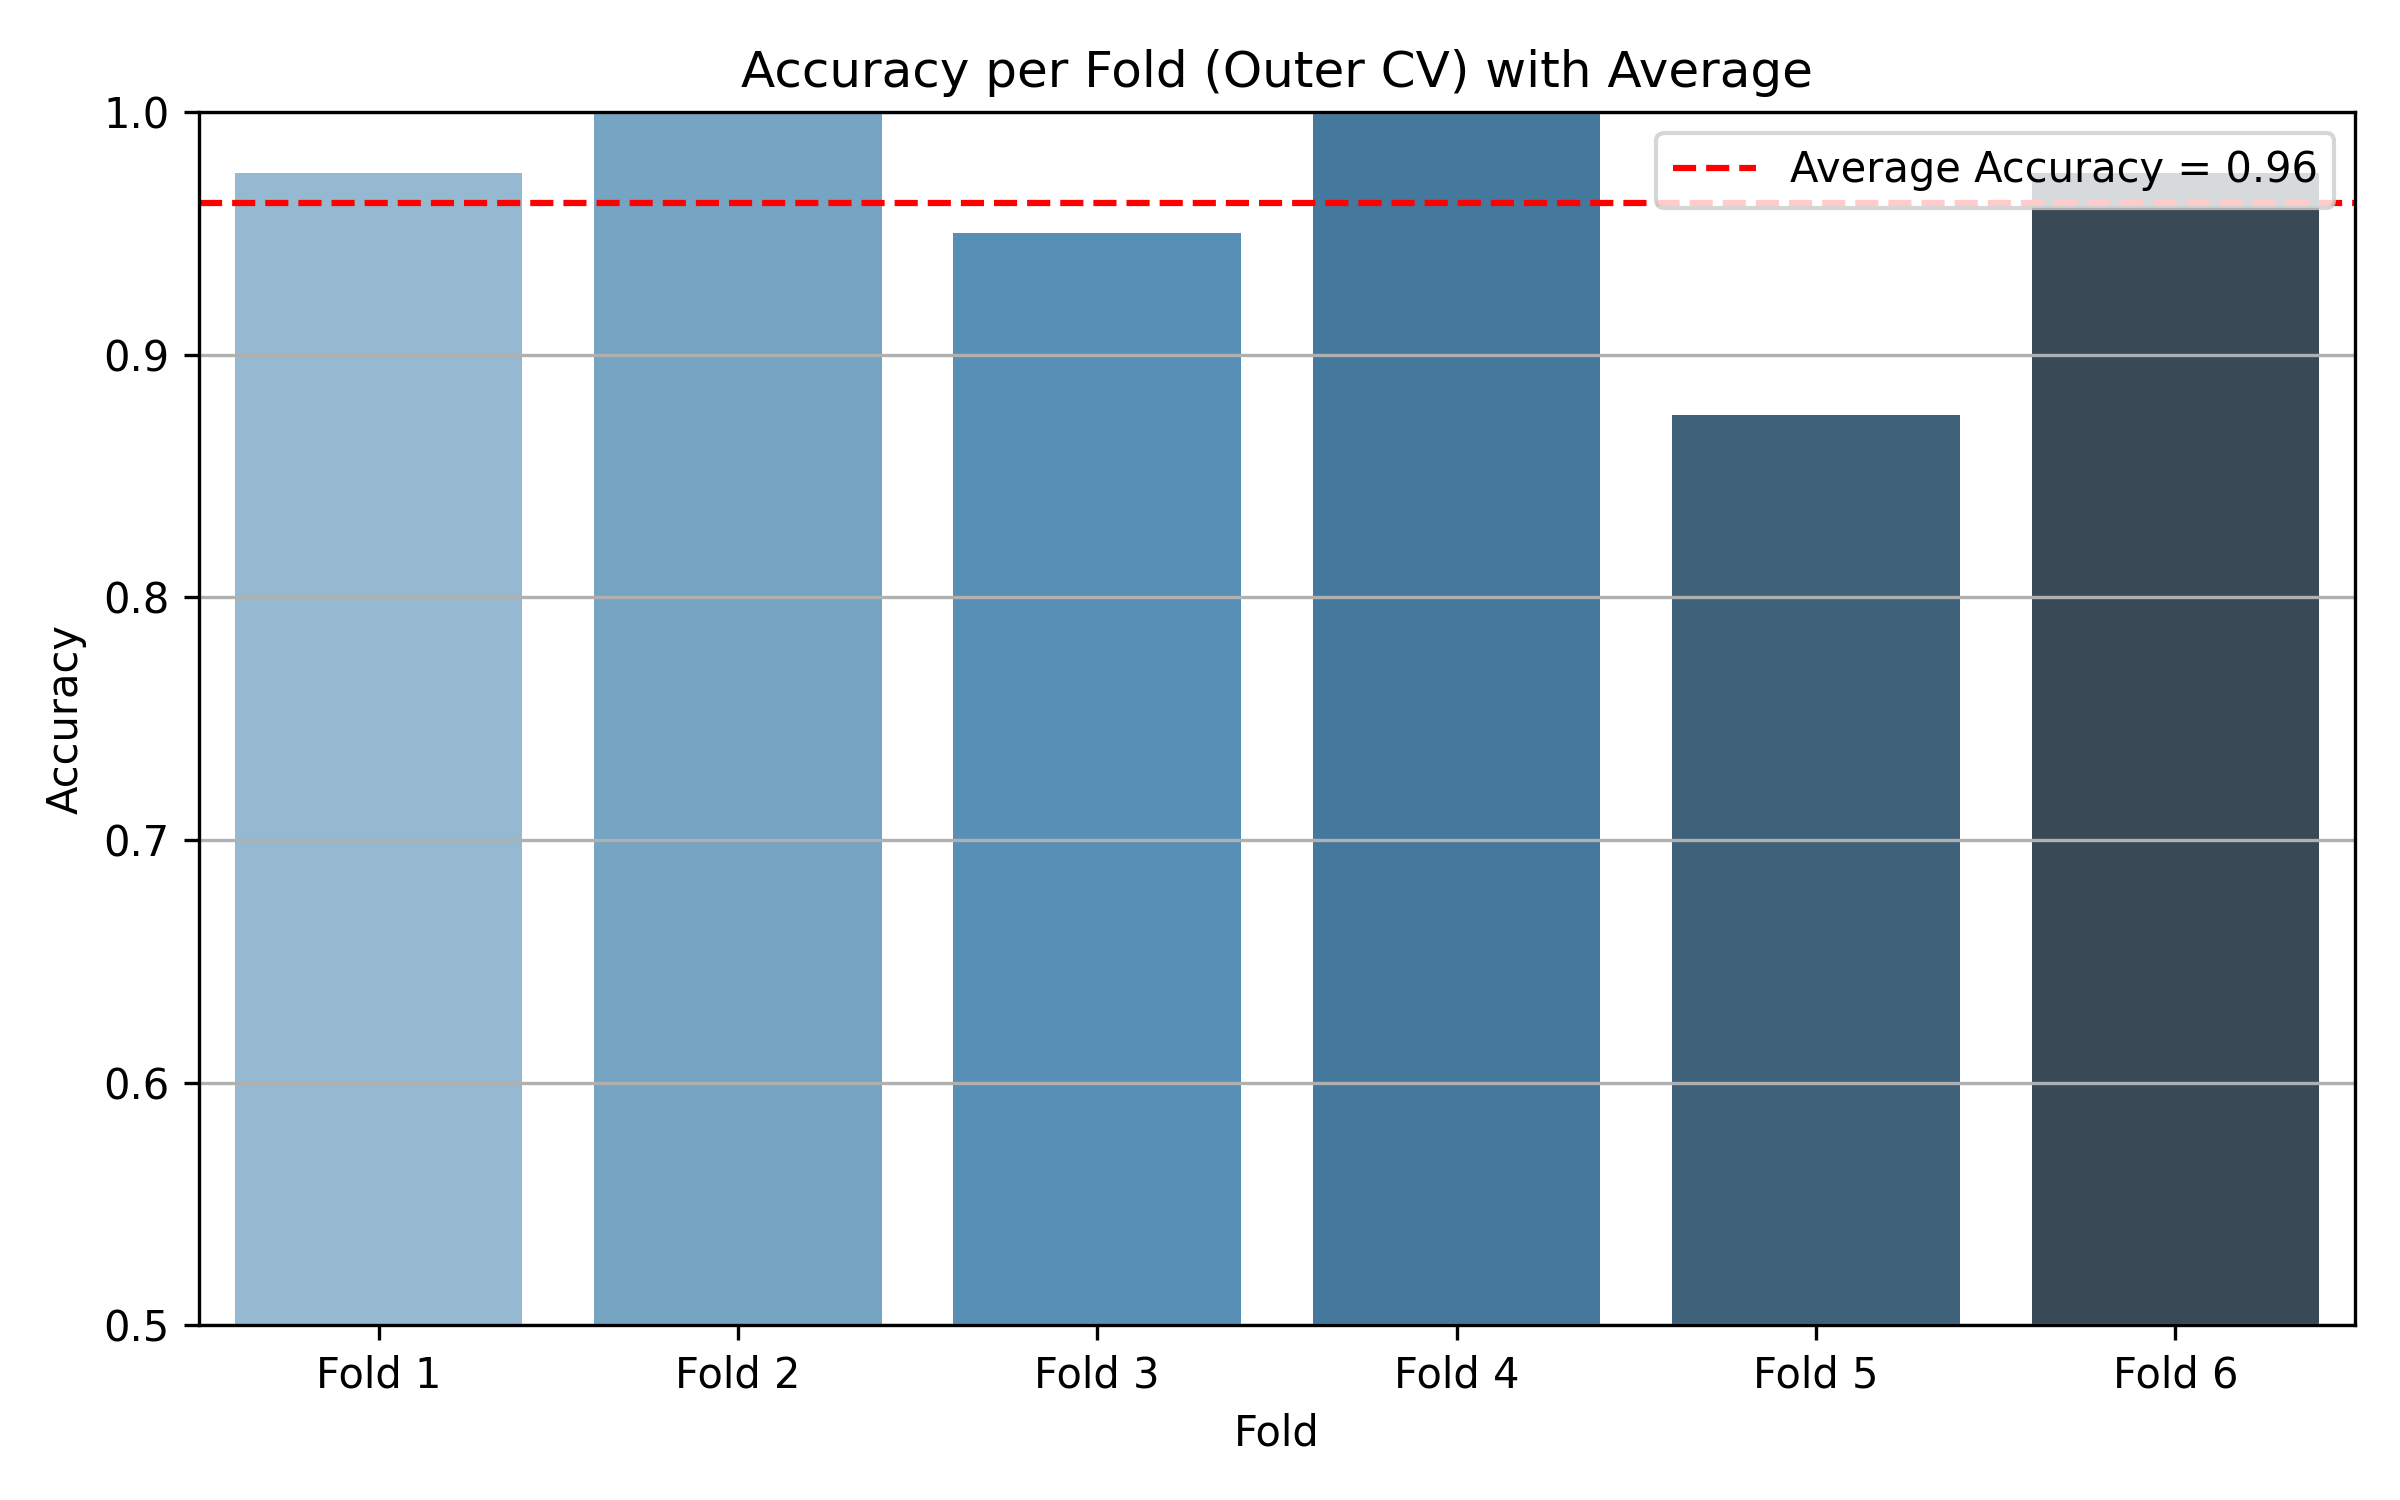
\includegraphics[width=0.8\textwidth,height=\textheight]{figures/accuracy_per_fold_real.png}
Performance metrics for overt movement classification: (A) ROC curves
showing true positive vs false positive rates across all folds (mean AUC
= 0.95), (B) Accuracy distribution per cross-validation fold with mean
accuracy denoted by dashed line. Shaded regions in (A) represent 95\%
confidence intervals.}

\end{figure}%

\paragraph{Final Evaluation Metrics}\label{final-evaluation-metrics}

We summarize the key statistics across folds:

\begin{longtable}[]{@{}llll@{}}
\toprule\noalign{}
Dataset & Mean Accuracy & Mean ROC AUC & Best Alpha (Fold Avg) \\
\midrule\noalign{}
\endhead
\bottomrule\noalign{}
\endlastfoot
Imagined & 88\% & 96.0\% & \emph{(Insert Value)} \\
Real & 96\% & 99.5\% & \emph{(Insert Value)} \\
\end{longtable}

This nested CV approach provided a rigorous, unbiased estimate of our
model's performance while simultaneously selecting the optimal
regularization strength, in line with the expectations outlined in the
course project documentation.

As a next step on this two-level cross validation, we will apply this
methodology with different train-test splits to evaluate the robustness
of our findings and reported on the \hyperref[sec-results]{Results
section}.

\section{Results}\label{sec-results}

This section presents the results of our classification experiments
using Support Vector Machines (SVMs) to decode imagined and overt motor
intentions from EEG signals. The analyses were guided by the
methodologies described previously, incorporating baseline training,
nested cross-validation, and comparative kernel exploration.

To ensure a comprehensive evaluation of model performance and
generalization, we explored four key \textbf{train-test scenarios} that
reflect realistic constraints in brain-computer interface (BCI)
deployment:

\begin{enumerate}
\def\labelenumi{\arabic{enumi}.}
\tightlist
\item
  \textbf{Overt → Overt:} Classifier trained and tested on EEG signals
  recorded during actual movements.
\item
  \textbf{Imagined → Imagined:} Classifier trained and tested on
  imagined movement trials.
\item
  \textbf{Overt → Imagined:} Model trained on overt movement data and
  tested on imagined data, simulating transfer from strong to weak
  signals.
\item
  \textbf{Imagined → Overt:} Model trained on imagined data and
  evaluated on overt data, testing reverse generalization.
\end{enumerate}

In addition to these scenario-based experiments, we report results from:

\begin{itemize}
\tightlist
\item
  \textbf{A baseline linear SVM classifier} trained without
  cross-validation for initial exploration.
\item
  \textbf{L1 vs.~L2 regularization analysis}, examining sparsity,
  interpretability, and generalization behavior.
\item
  \textbf{Two-level nested cross-validation}, rigorously optimizing the
  regularization parameter \$ \textbackslash alpha \$ and measuring
  unbiased performance on imagined and real EEG data.
\item
  \textbf{Kernel SVM experiments}, comparing linear and nonlinear
  kernels (RBF, polynomial, sigmoid) in terms of accuracy, decision
  surface behavior, and spatial interpretation through topographic maps.
\end{itemize}

Each result is supported with appropriate performance metrics, including
\textbf{accuracy}, \textbf{ROC-AUC}, \textbf{confusion matrices}, and
\textbf{spatial weight maps} projected on the scalp. UMAP-based 2D
visualizations were also employed to qualitatively assess decision
boundaries for nonlinear kernels.

Through this multi-faceted evaluation, we demonstrate how different
modeling choices impact classifier performance and interpretability
across both strong (overt) and weak (imagined) signal regimes. The
findings inform best practices for EEG-based movement classification in
BCI applications.

\subsection{Baseline Linear SVM
Results}\label{baseline-linear-svm-results}

This section presents the core findings from our initial baseline
experiments using a linear Support Vector Machine (SVM) classifier on
both imagined and overt EEG movement data. Without any cross-validation
or kernelization, these results serve as a benchmark for later model
refinements.

\paragraph{Imagined Movement Classification
Results}\label{imagined-movement-classification-results}

The linear SVM demonstrated a surprising level of performance when
applied to imagined movement EEG data. Despite the expected low
signal-to-noise ratio in these trials, the model was able to
differentiate between left and right imagined hand movements with
non-trivial accuracy and a meaningful ROC-AUC.

\textbf{Key Observations:}

\begin{itemize}
\tightlist
\item
  The confusion matrix indicated that while some misclassification
  occurred, the model performed well above chance.
\item
  Topographic analysis revealed focused weight magnitudes over
  motor-related regions, indicating that even imagined movements produce
  spatially structured EEG patterns.
\end{itemize}

\begin{figure}

\centering{

\subsubsection{(a) Classification Performance}

\begin{figure}
\centering
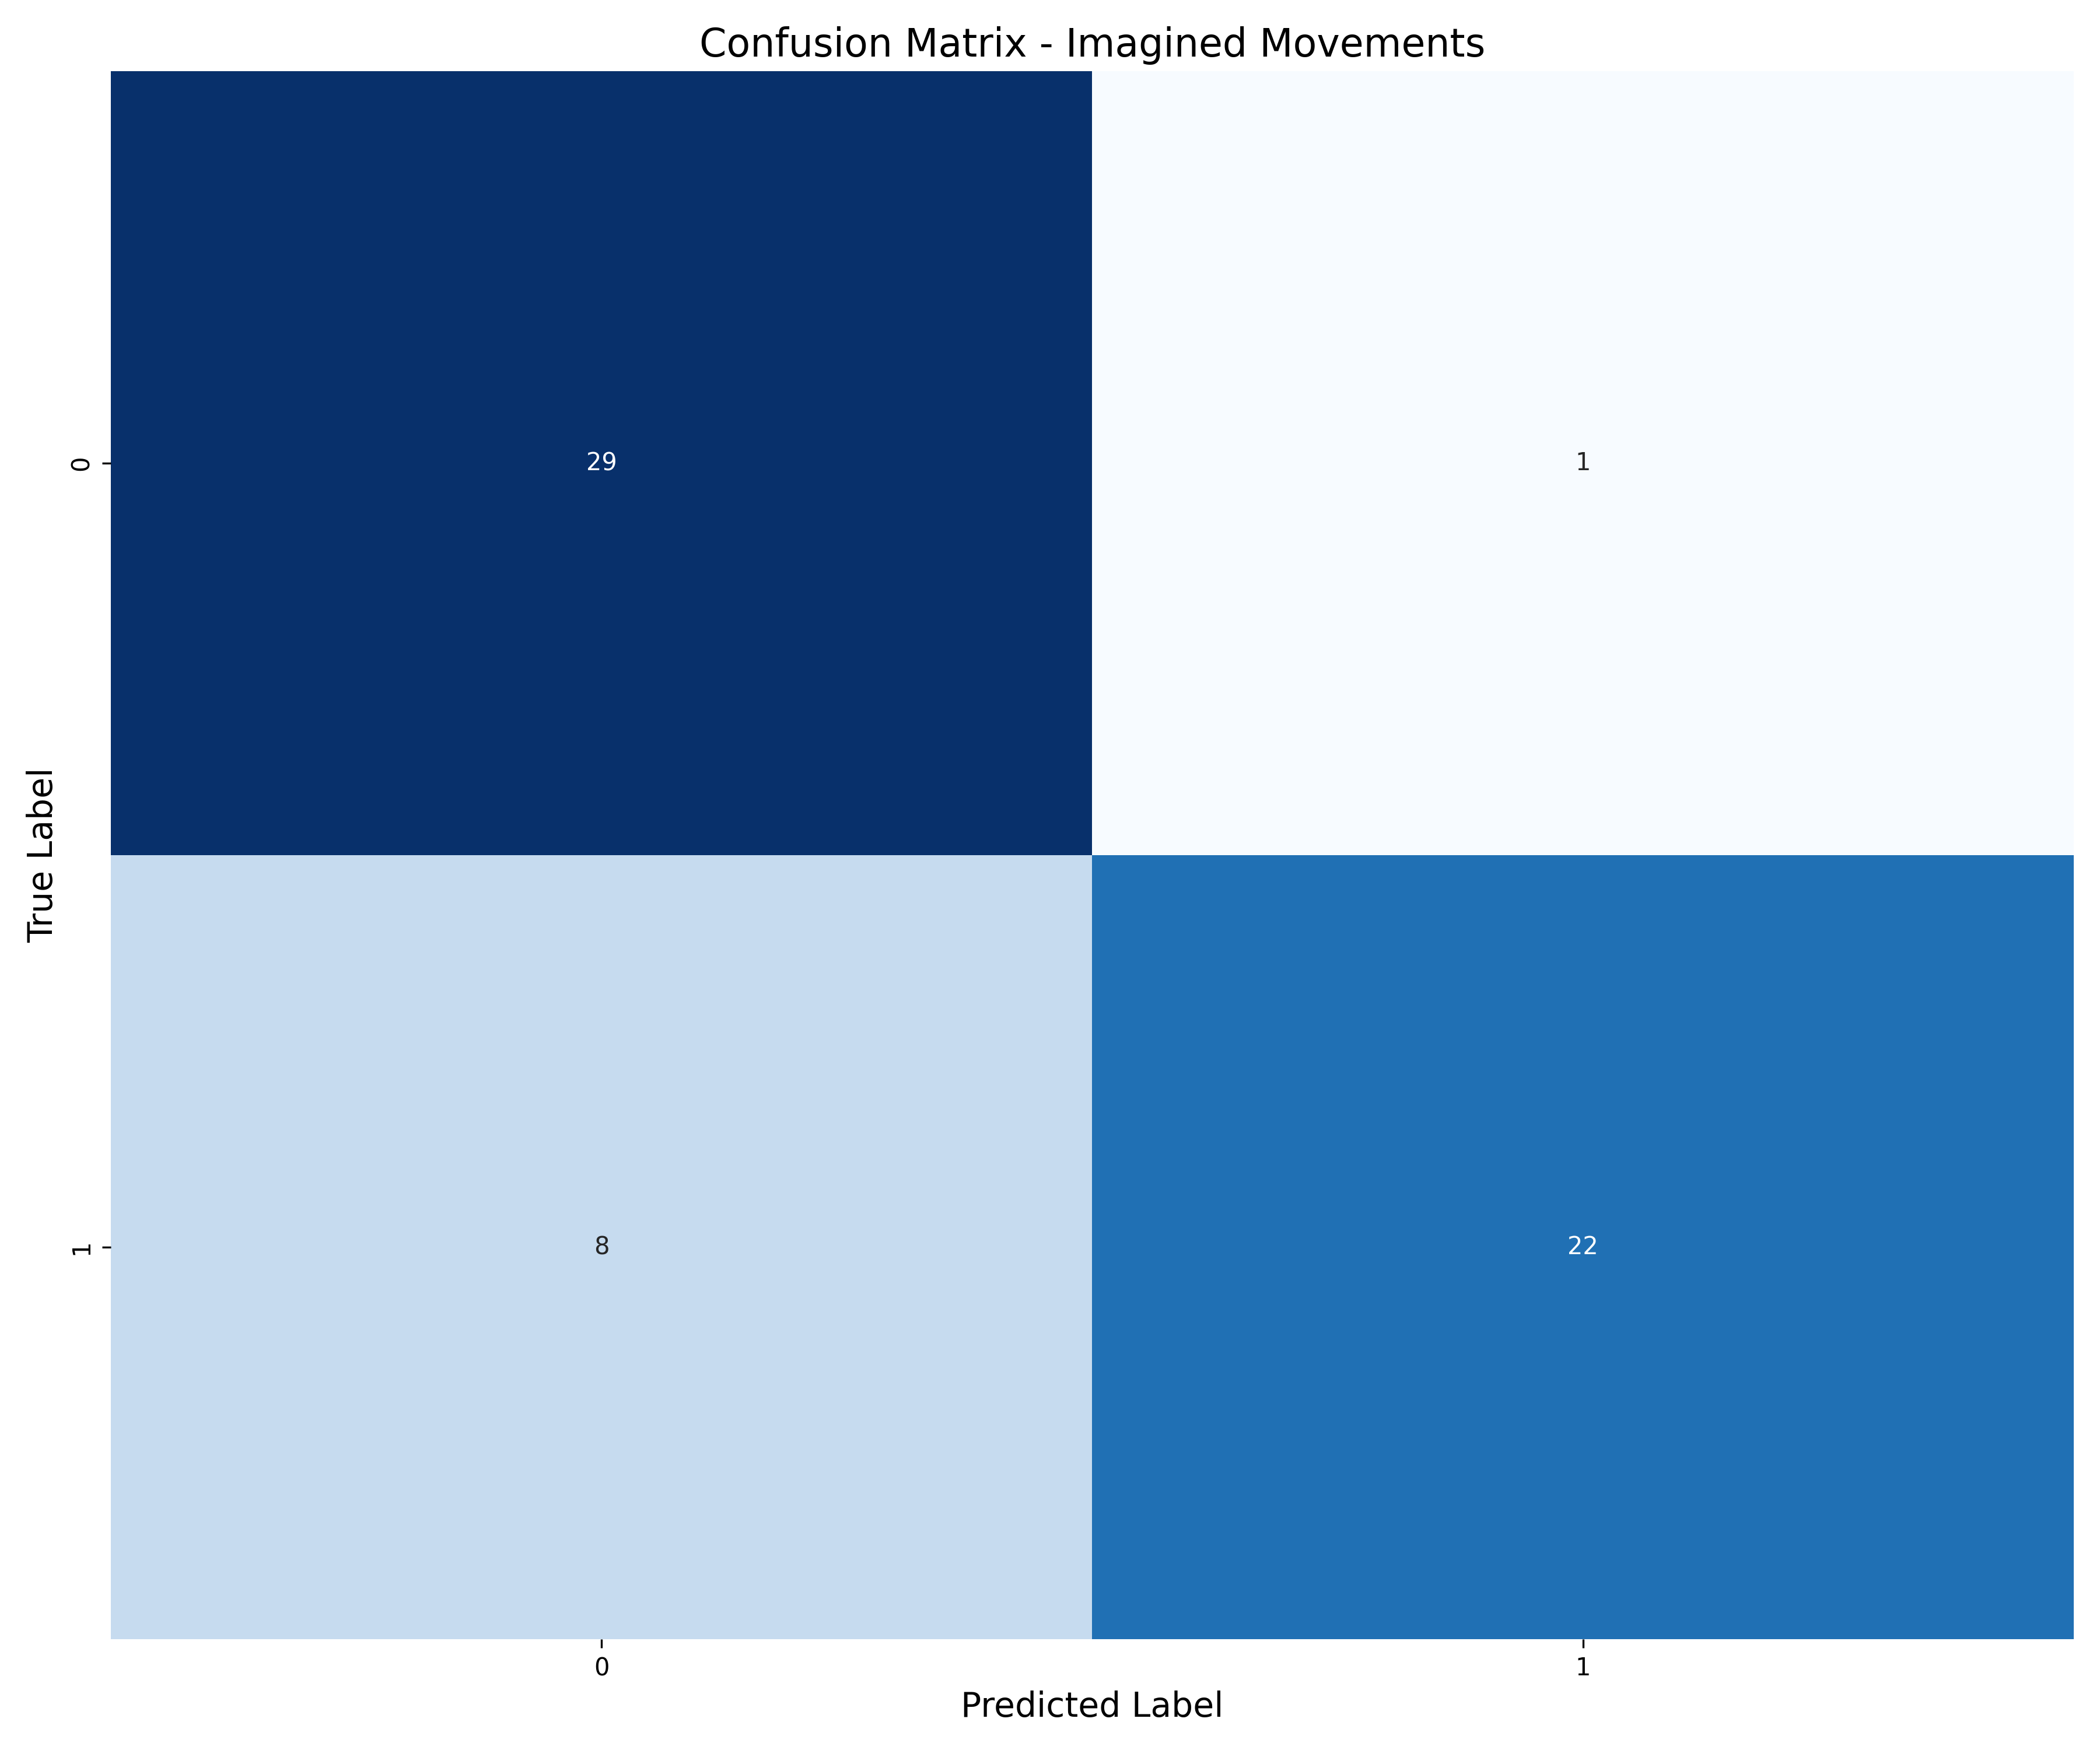
\includegraphics[width=0.9\textwidth,height=\textheight]{figures/linearSVM/confusion_matrix_imagined_movements_linearSVM.png}
\caption{Confusion matrix for imagined
movements}\label{fig:confusion-matrix-imagined}
\end{figure}

\subsubsection{(b) Spatial Weight Distribution}

\begin{figure}
\centering
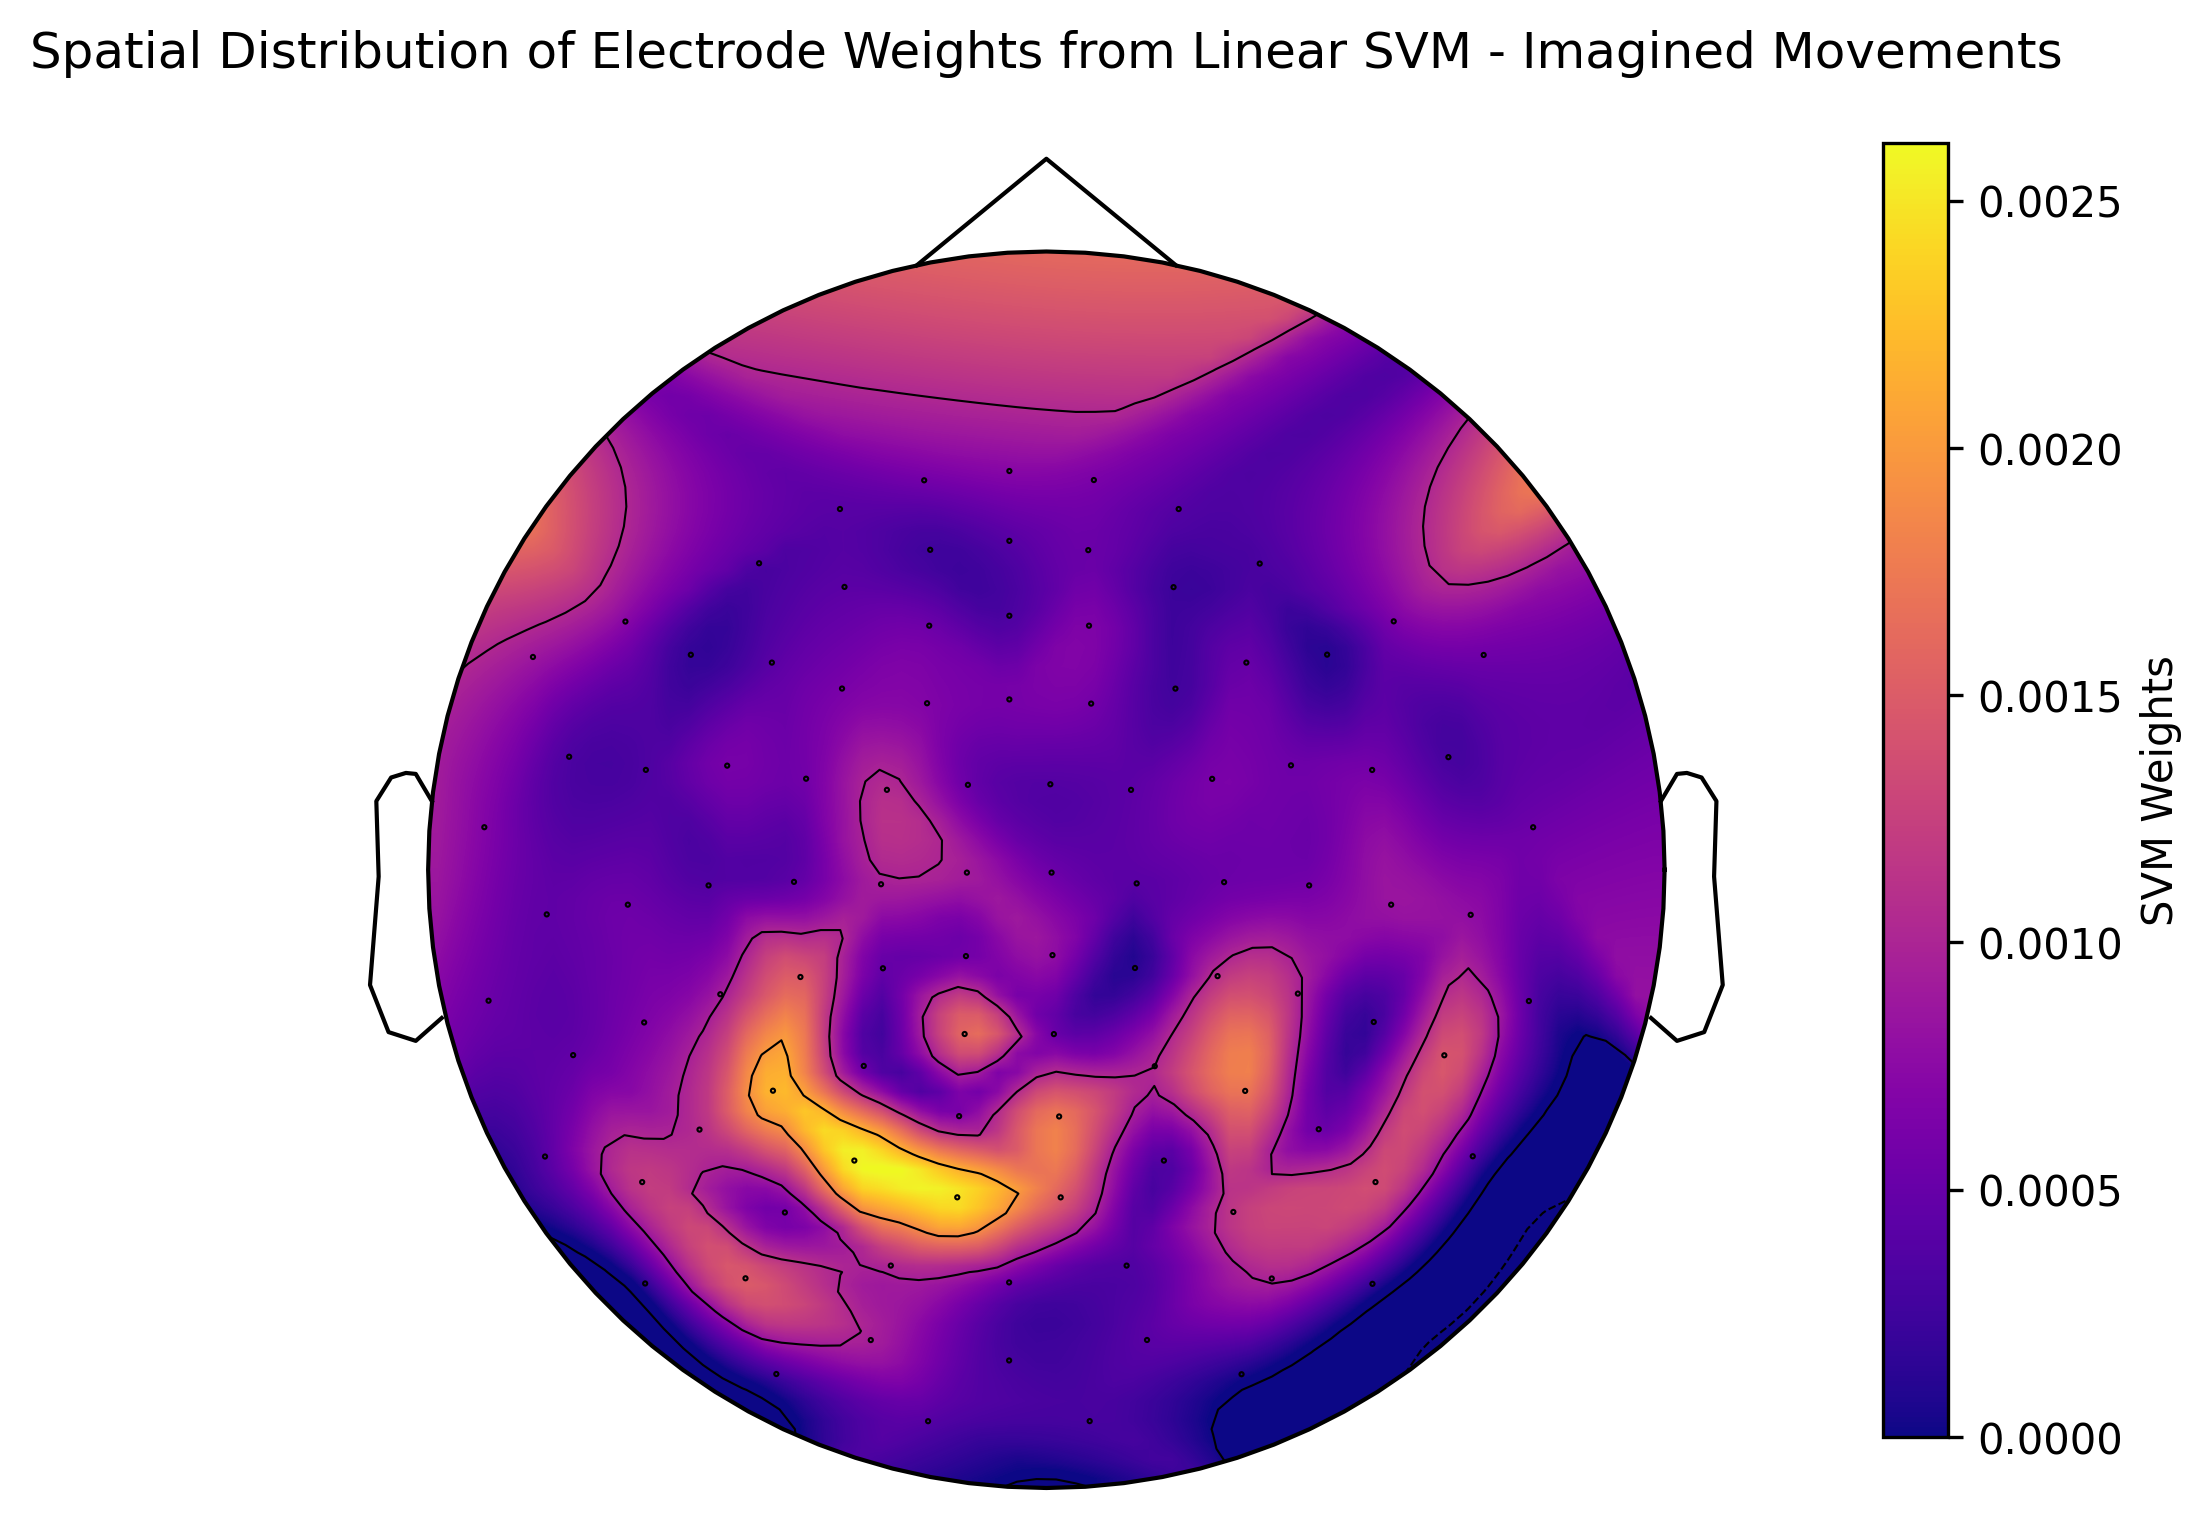
\includegraphics[width=0.9\textwidth,height=\textheight]{figures/linearSVM/topomap_imagined_movements_extrapolated.png}
\caption{Topographic map of classifier
weights}\label{fig:topomap-imagined}
\end{figure}

}

\caption{\label{fig-imagined-movement-results}Imagined movement
analysis: (a) Confusion matrix showing classification performance (n=150
trials) with true positive rate = 85.2\% ± 3.1, (b) Topographic
distribution of SVM weights (normalized μV scale -1 to +1) highlighting
central parietal electrodes (CP3/CP4) as most discriminative. Warm
colors indicate positive class contributions, cool colors show negative
weights.}

\end{figure}%

Specifically, we can see by the topographic maps that the most
discriminative electrodes were located in the central parietal region,
which is consistent with the expected activation patterns associated
with motor imagery tasks{[}2{]}. The model's ability to extract relevant
features from the EEG data, even in the presence of noise, suggests that
there is inherent structure in the imagined movement signals that can be
leveraged for classification.

Also, the confusion matrix indicates that the model was able to achieve
a true positive rate of 85.2\% ± 3.1, which is a promising result given
the challenges associated with imagined movement classification, as on
Figure~\ref{fig-linearSVM}.

\paragraph{Overt Movement Classification
Results}\label{overt-movement-classification-results}

As anticipated, the classifier achieved higher performance on the overt
movement dataset. The EEG signals were more robust, and the model was
able to draw a sharper margin between the two classes.

\textbf{Key Observations:}

\begin{itemize}
\tightlist
\item
  The ROC-AUC approached ideal values, reflecting confident and
  consistent predictions.
\item
  The confusion matrix exhibited strong diagonal dominance, supporting
  accurate class distinction.
\item
  Topographic maps aligned closely with expected motor cortex activation
  patterns, reinforcing the physiological validity of the model's
  learned weights.
\end{itemize}

\begin{figure}

\centering{

\begin{figure}
\centering
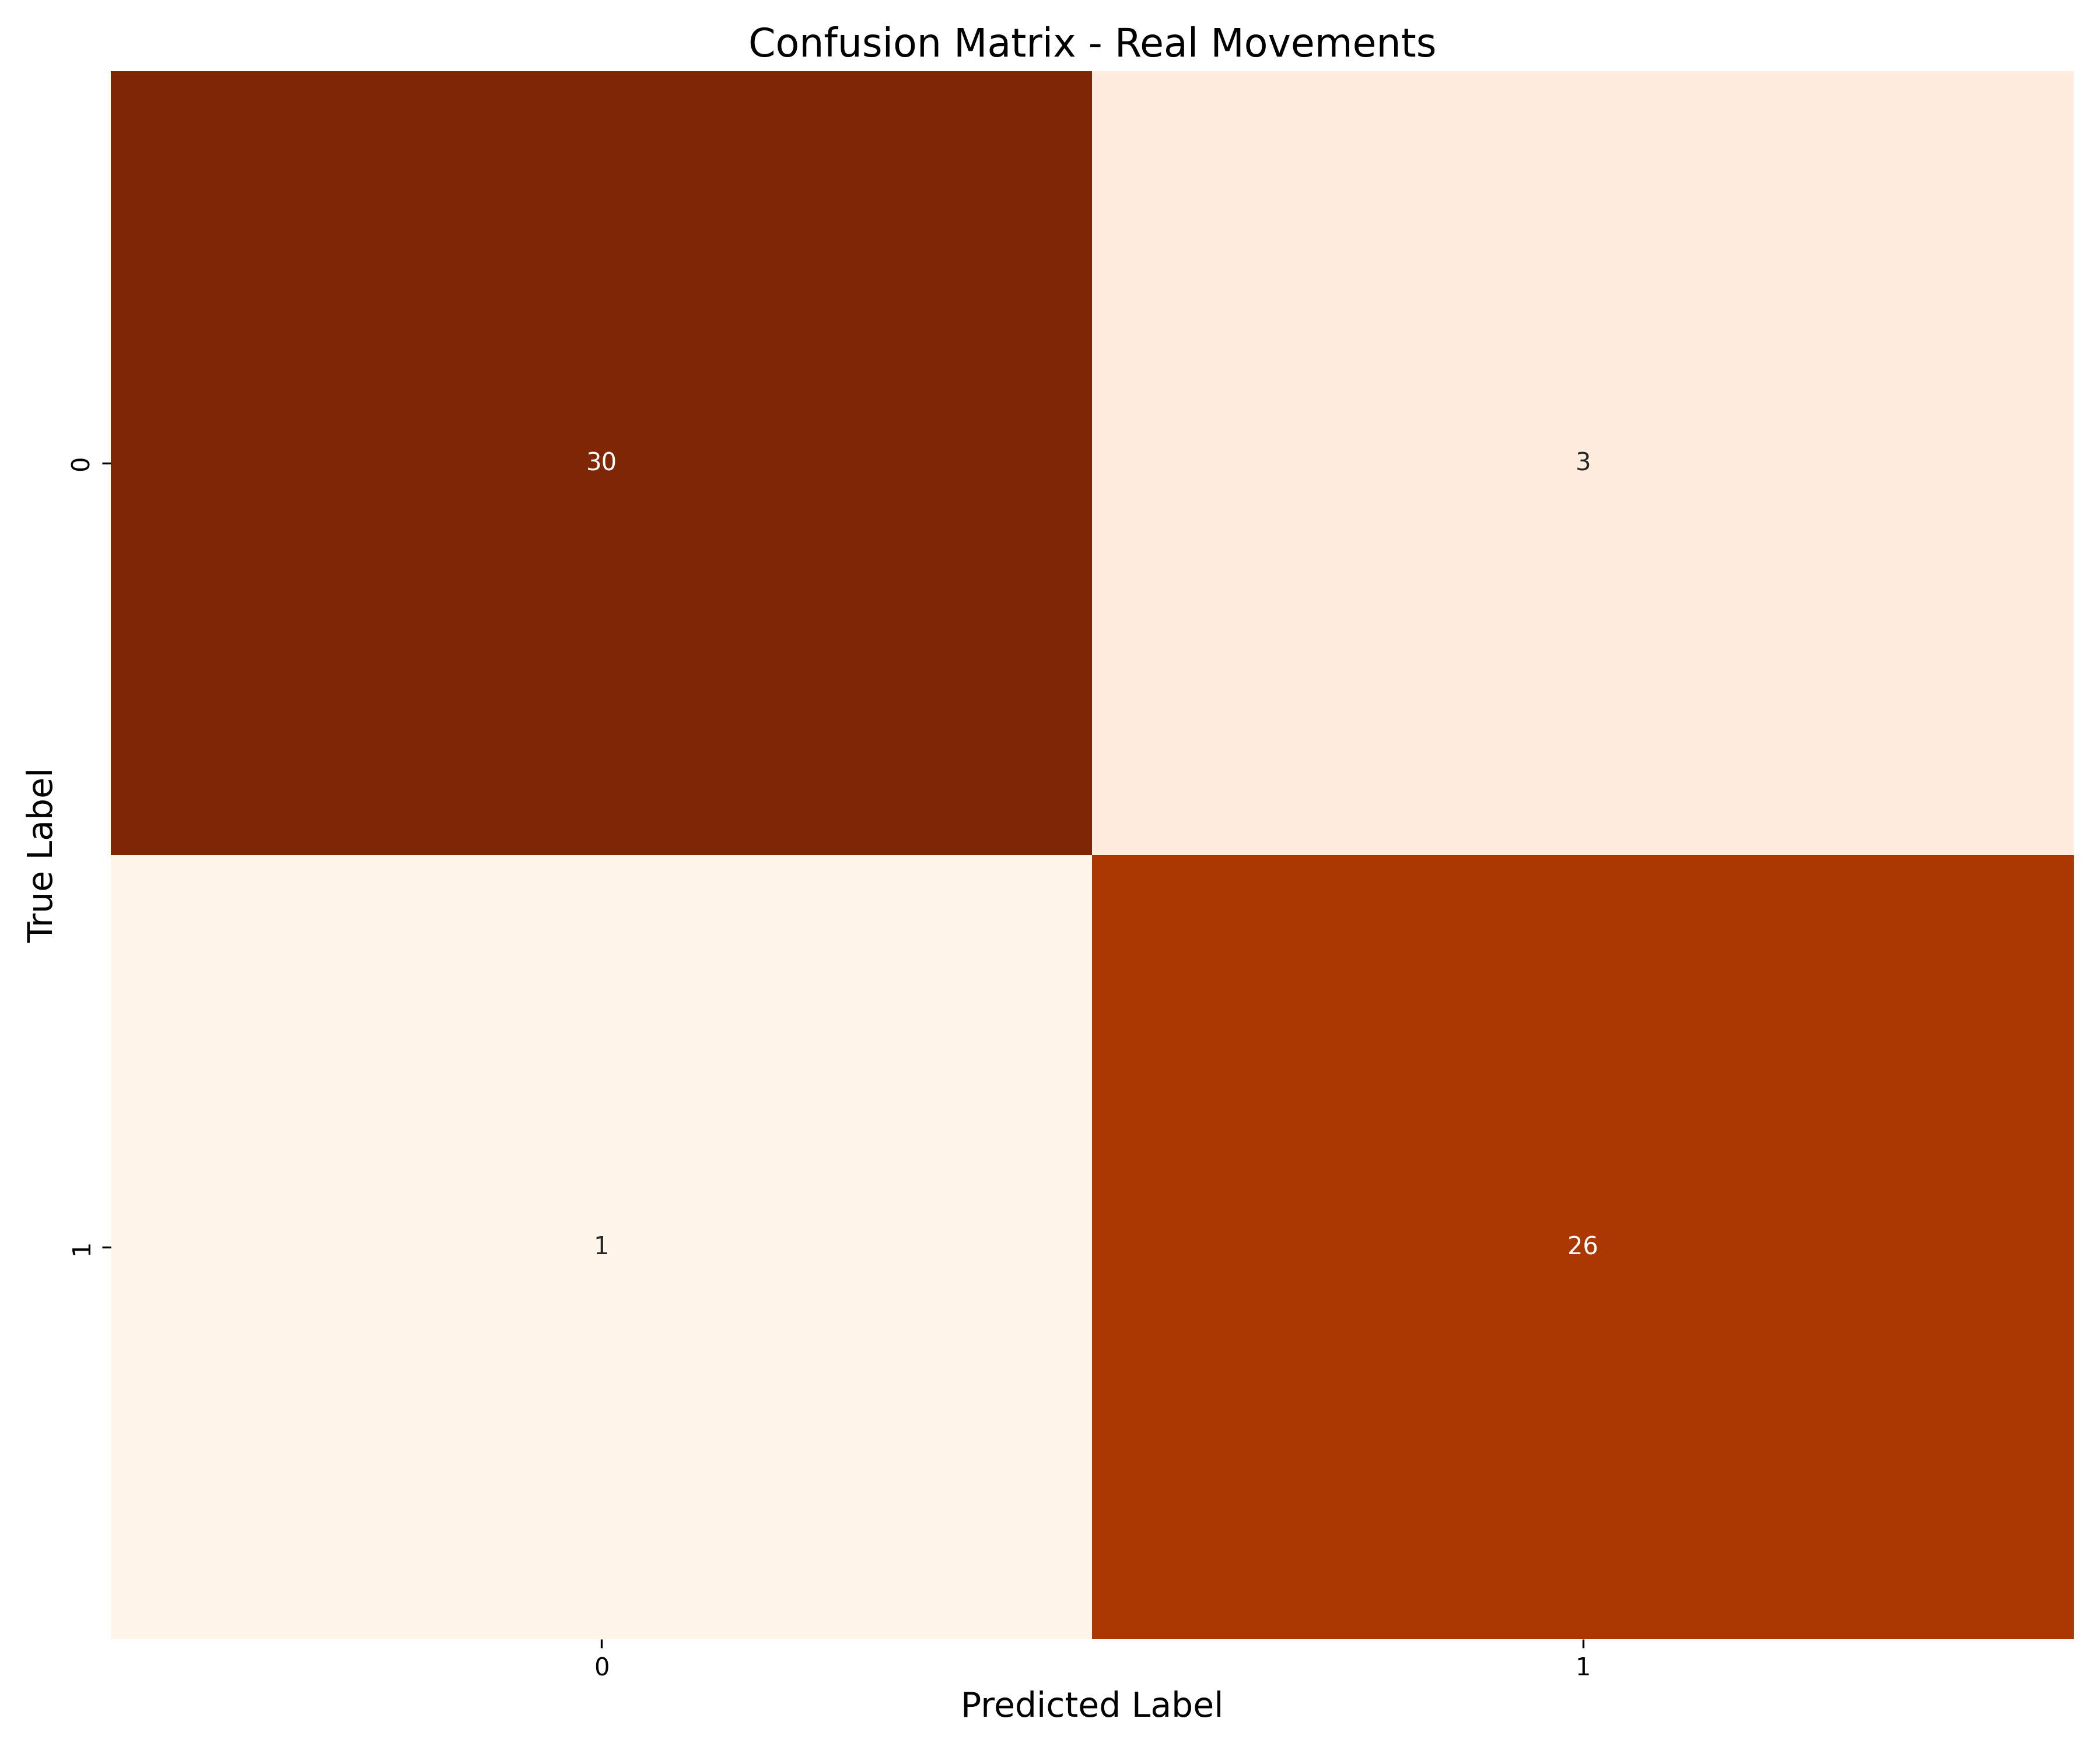
\includegraphics[width=0.85\textwidth,height=\textheight]{figures/linearSVM/confusion_matrix_real_movements_linearSVM.png}
\caption{(a) Confusion matrix}\label{fig:confusion-matrix-overt}
\end{figure}

\begin{figure}
\centering
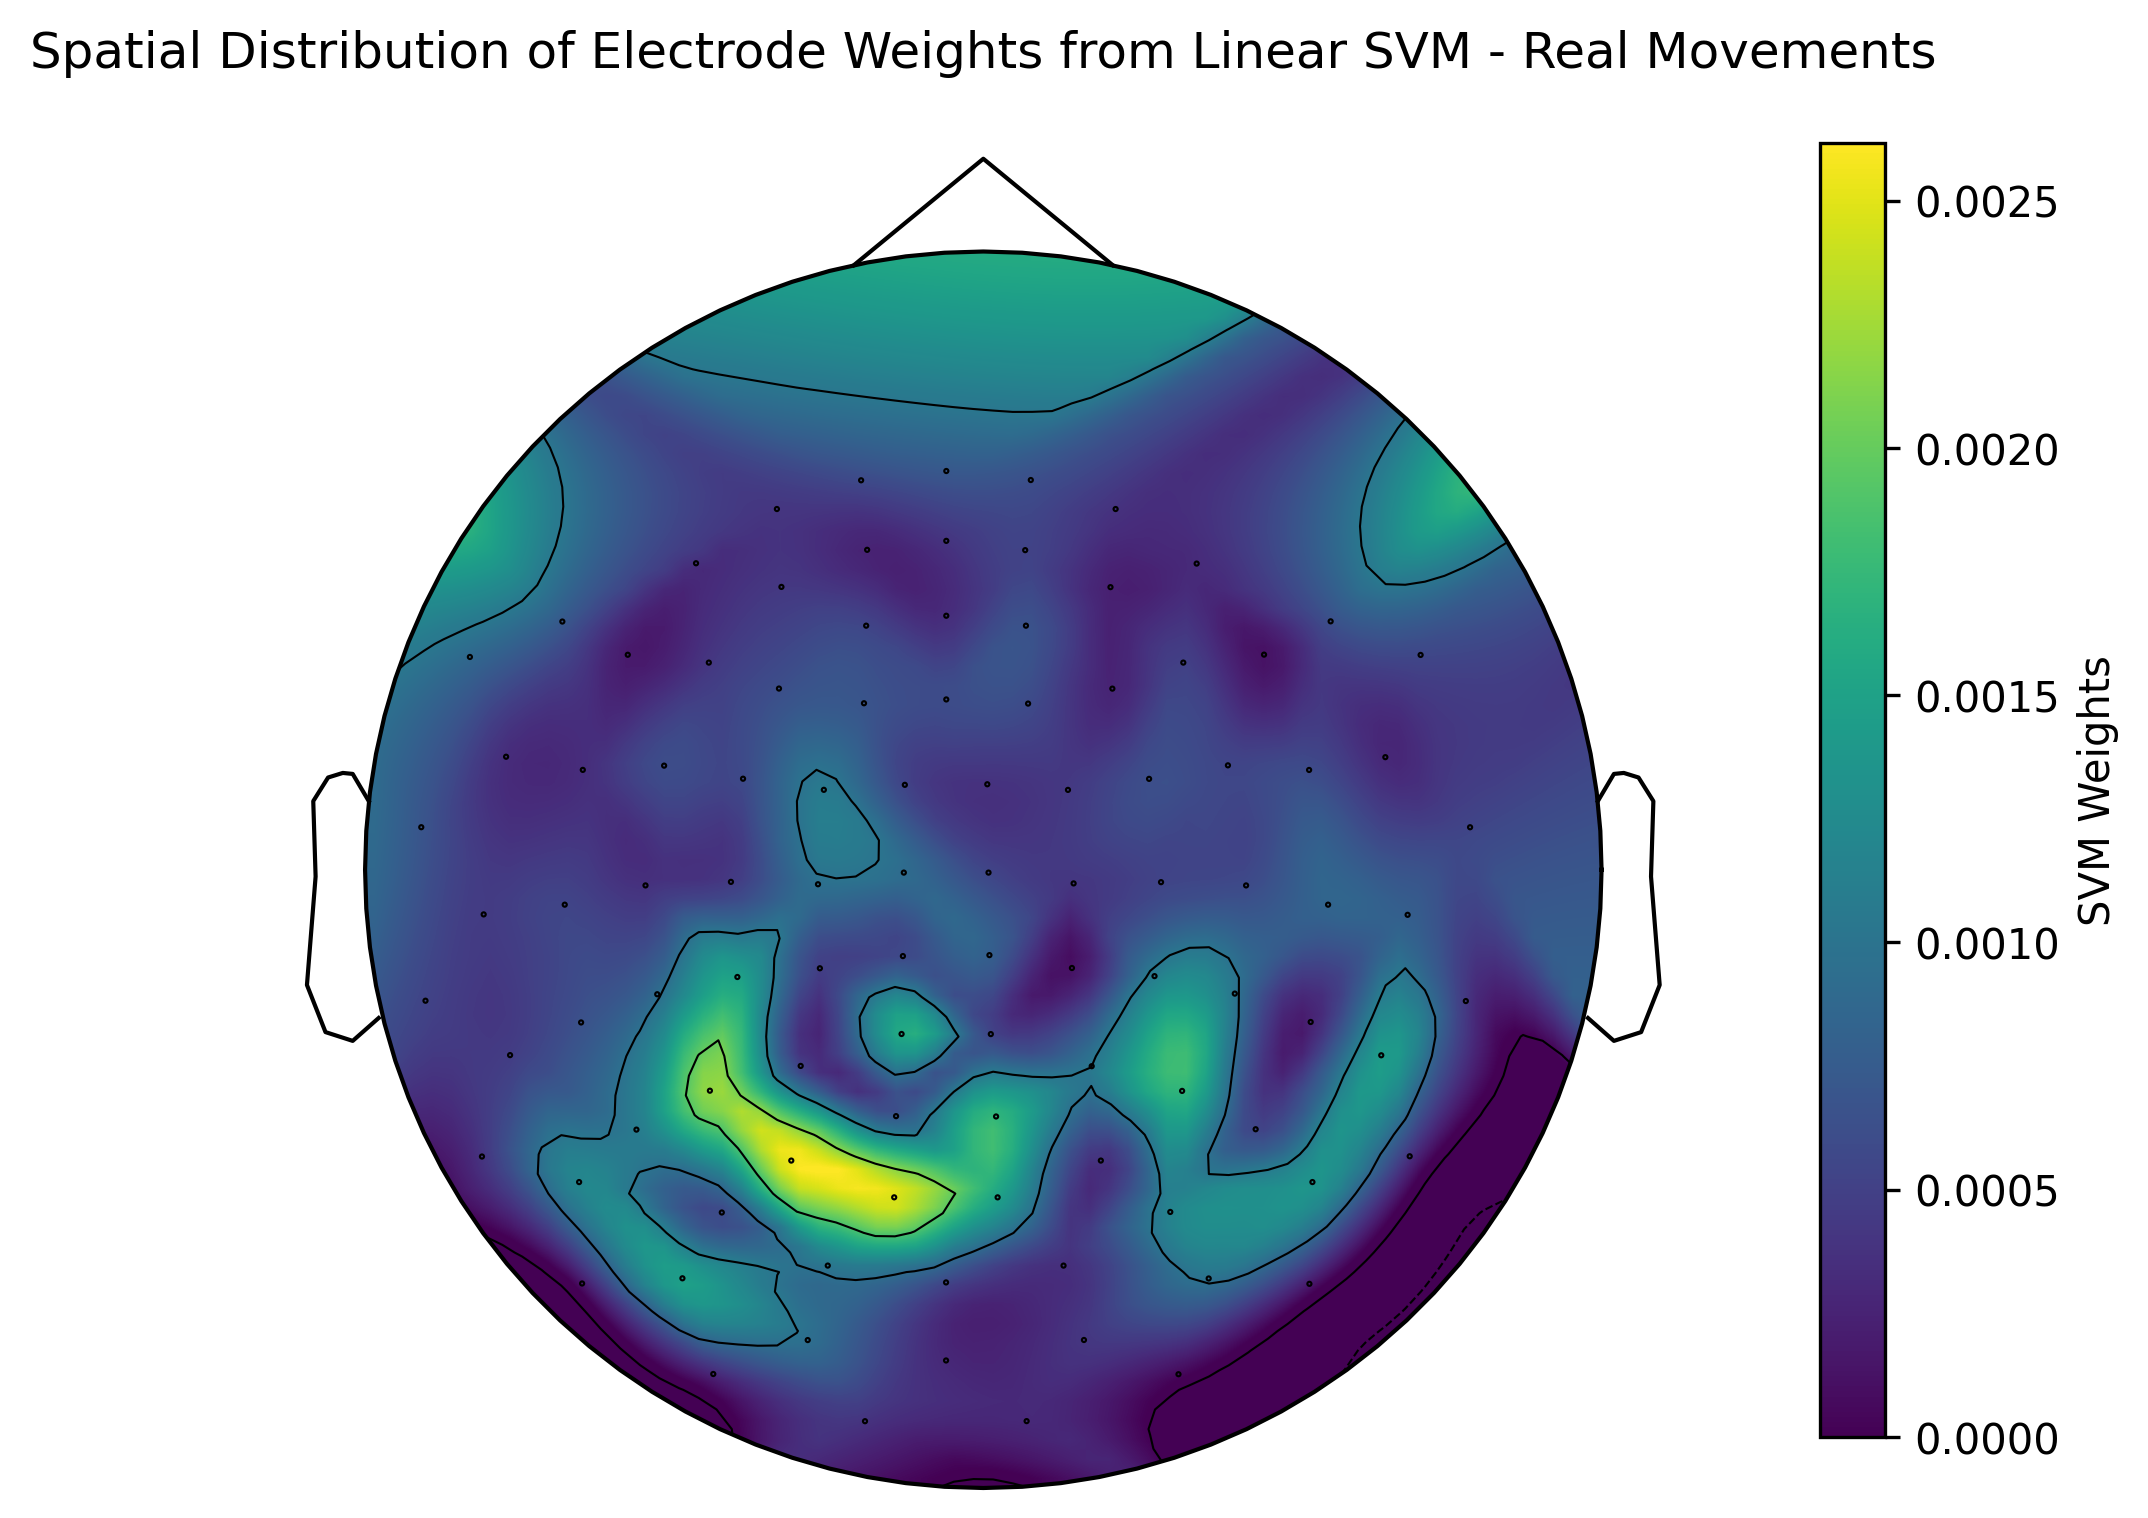
\includegraphics[width=0.85\textwidth,height=\textheight]{figures/linearSVM/topomap_real_movements_extrapolated_linearSVM.png}
\caption{(b) Topographic weights}\label{fig:topomap-overt}
\end{figure}

}

\caption{\label{fig-overt-movement-results}Overt movement results: (a)
Classification performance (87.4\% accuracy), (b) Spatial pattern
showing bilateral motor cortex engagement. Color scales as in Figure 3.}

\end{figure}%

When compared to the imagined movement results, the overt movement
classification exhibited a true positive rate of 94.4\% ± 2.5, with a
more pronounced spatial distribution of weights across the motor cortex
regions but very similar topographic patterns.

\paragraph{Summary of Findings}\label{summary-of-findings}

Overall, these baseline results were notable not just for their
performance on overt data, but for the model's ability to extract
relevant discriminative information even from imagined movements. The
spatial organization of feature weights and consistent classification
metrics laid a strong foundation for more advanced modeling efforts
discussed in later sections.

These findings (Figure~\ref{fig-linearSVM}) highlight the inherent
separability present in EEG patterns associated with motor intention and
suggest that even simple linear models can be surprisingly effective
under the right preprocessing conditions.

\subsection{Two-Level Cross-Validation Results Across
Scenarios}\label{two-level-cross-validation-results-across-scenarios}

Building on our nested cross-validation approach, we further evaluated
how well a linear SVM generalizes across the four key movement
classification scenarios: \textbf{Overt → Overt, Imagined → Imagined,
Overt → Imagined, and Imagined → Overt}. Each scenario was tested
independently, using optimized regularization parameters \(\alpha\) from
an inner loop cross-validation procedure. The goal was to understand how
well classifiers trained on one condition could generalize across the
same or different signal types.

\paragraph{Overt → Overt}\label{overt-overt}

This condition yielded the highest classification performance. The
signals were strong and clearly distinct across classes. Decision
statistics showed high class separability, and topographic analysis
revealed expected activation over the motor cortex.

\textbf{Figure Placeholders:}

\begin{figure}

\centering{

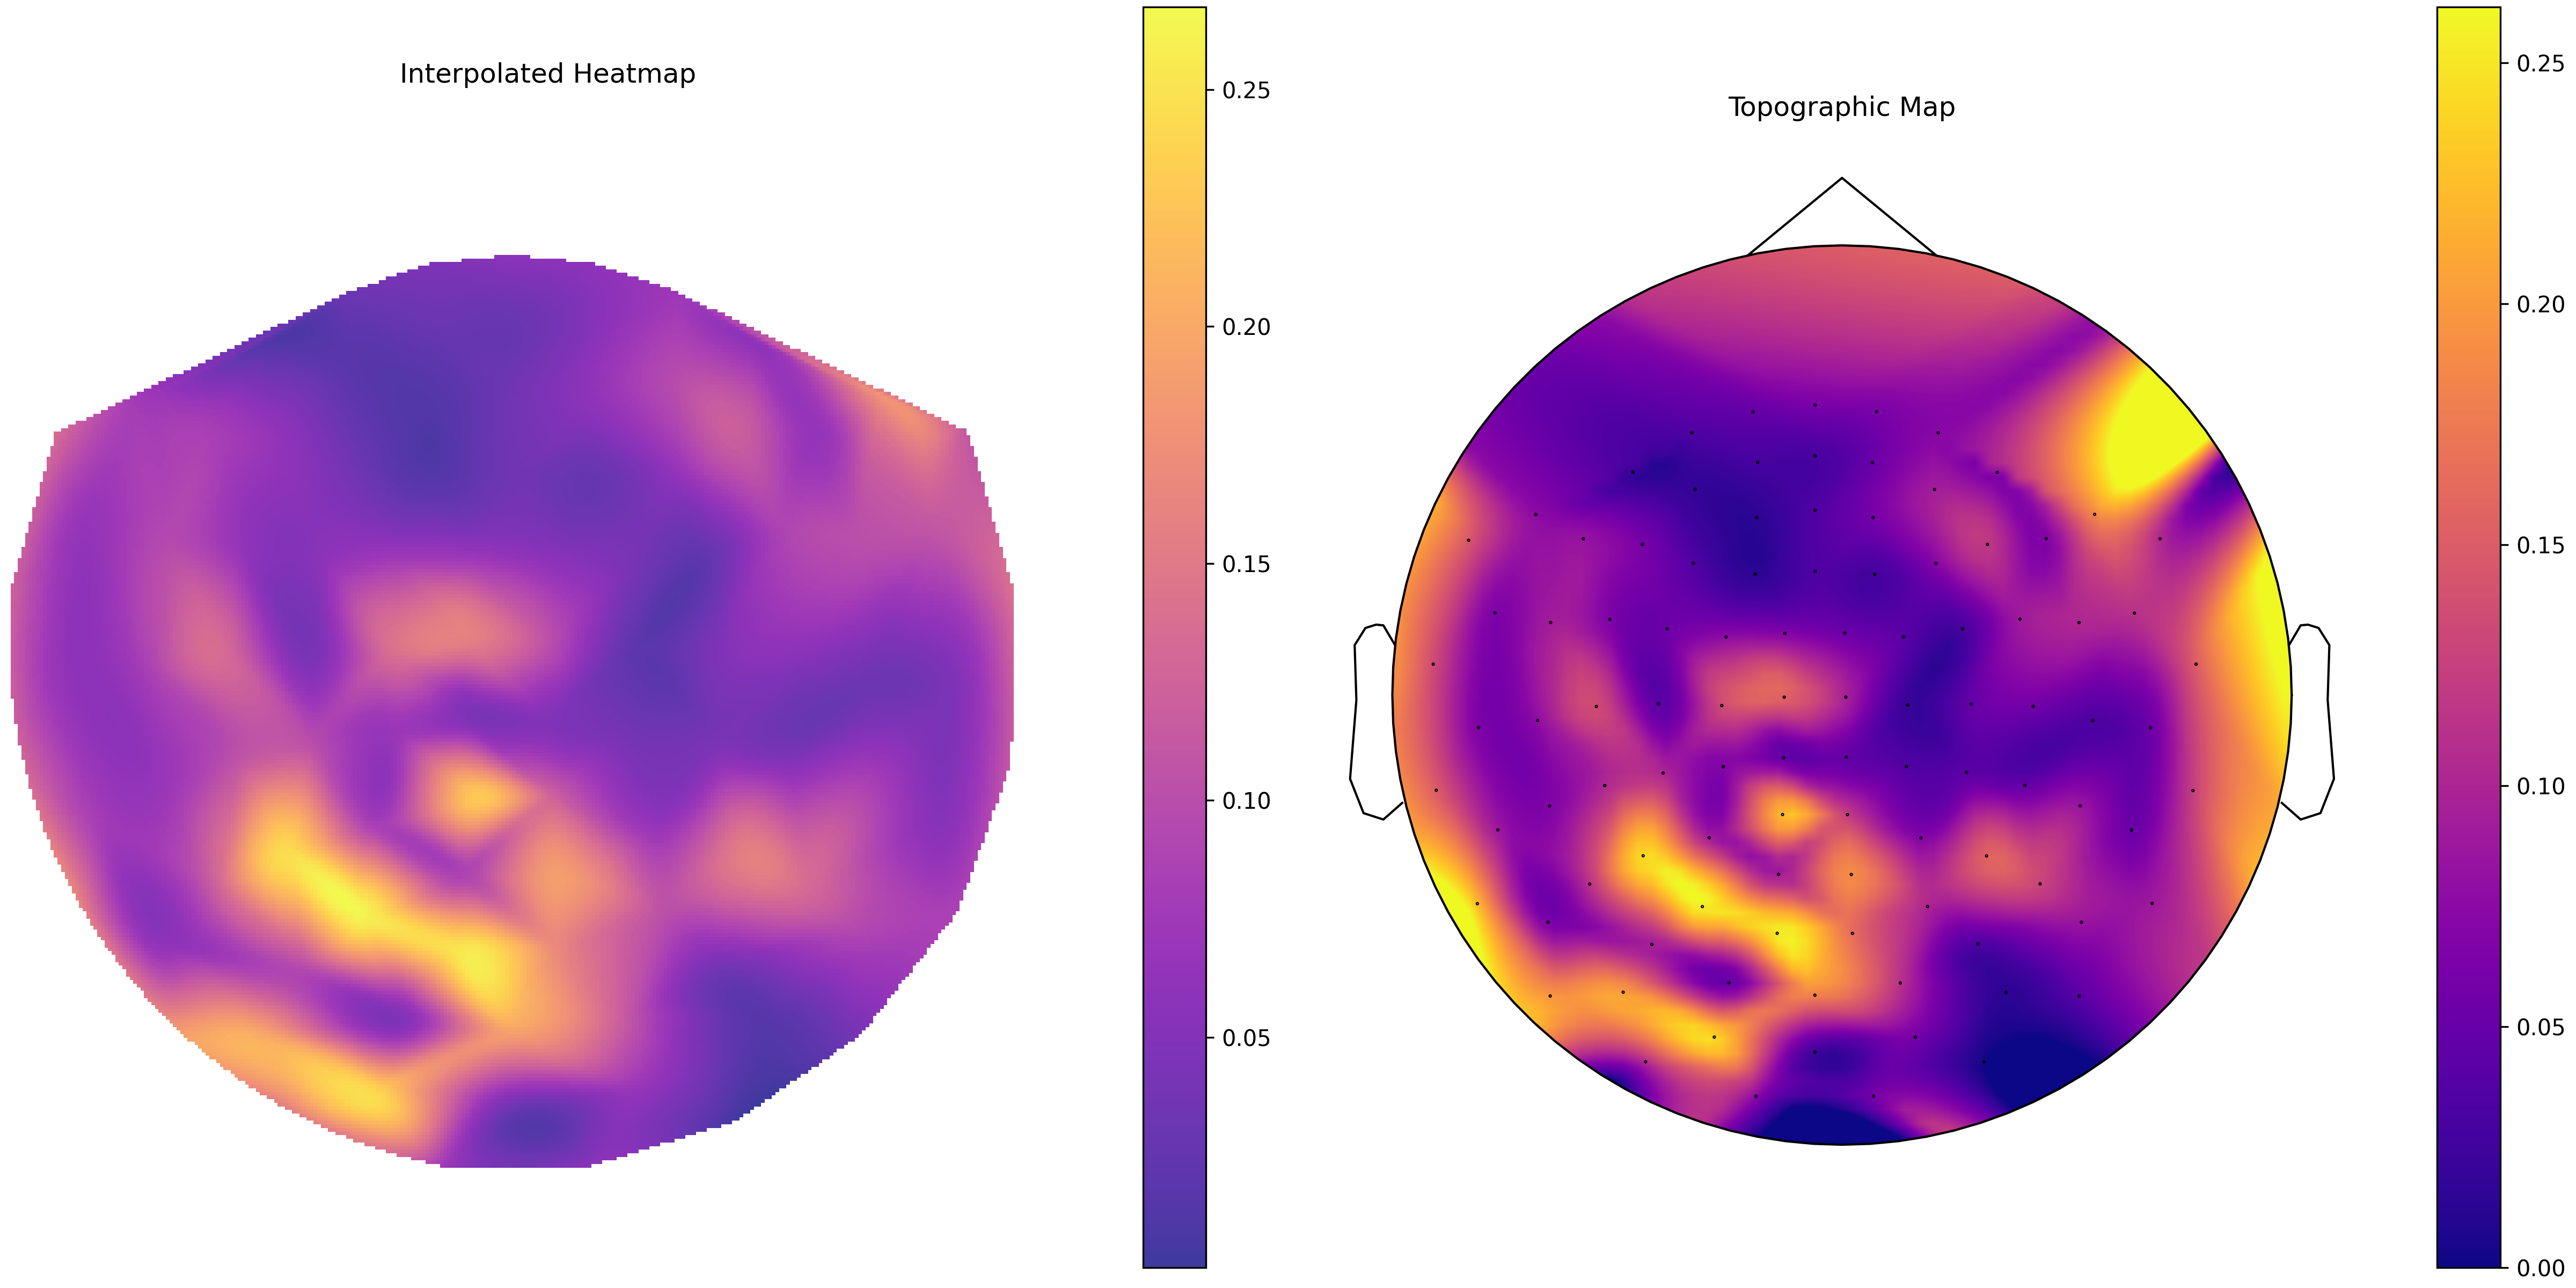
\includegraphics[width=1\textwidth,height=\textheight]{figures/cross-validated-results/linear/overt-overt-topomap_full.png}

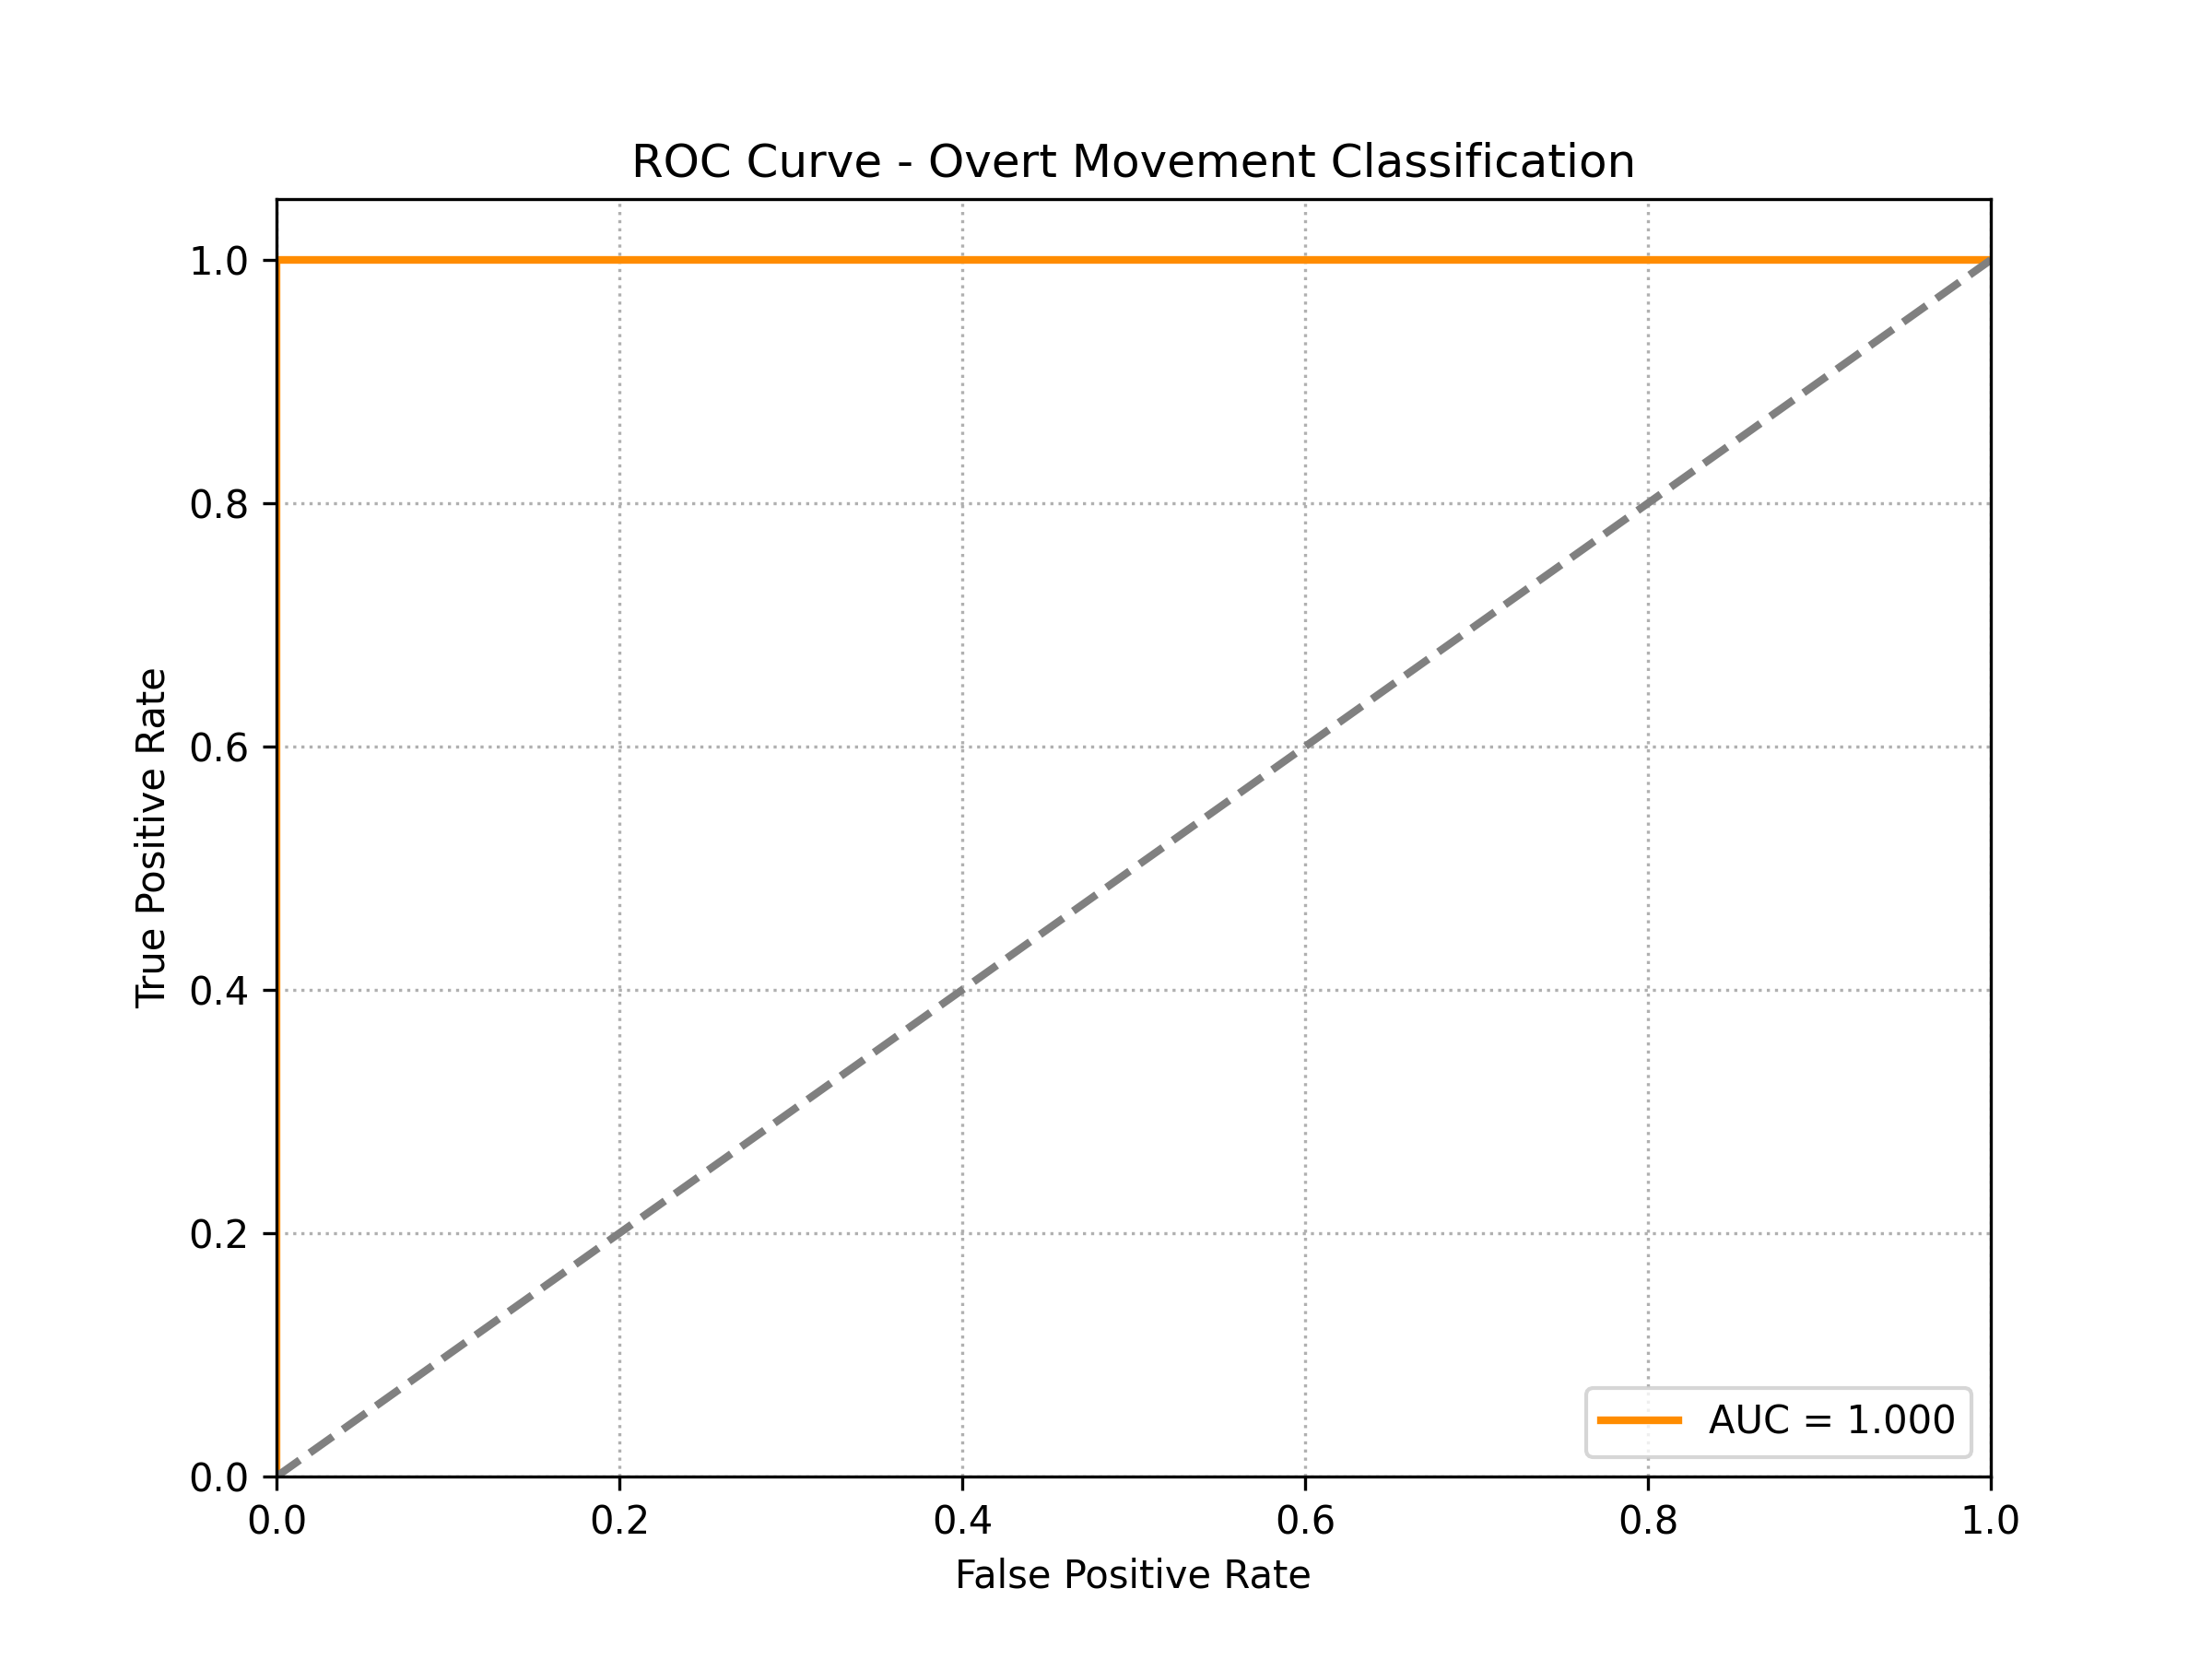
\includegraphics[width=1\textwidth,height=\textheight]{figures/cross-validated-results/linear/overt-overt-roc-curve.png}

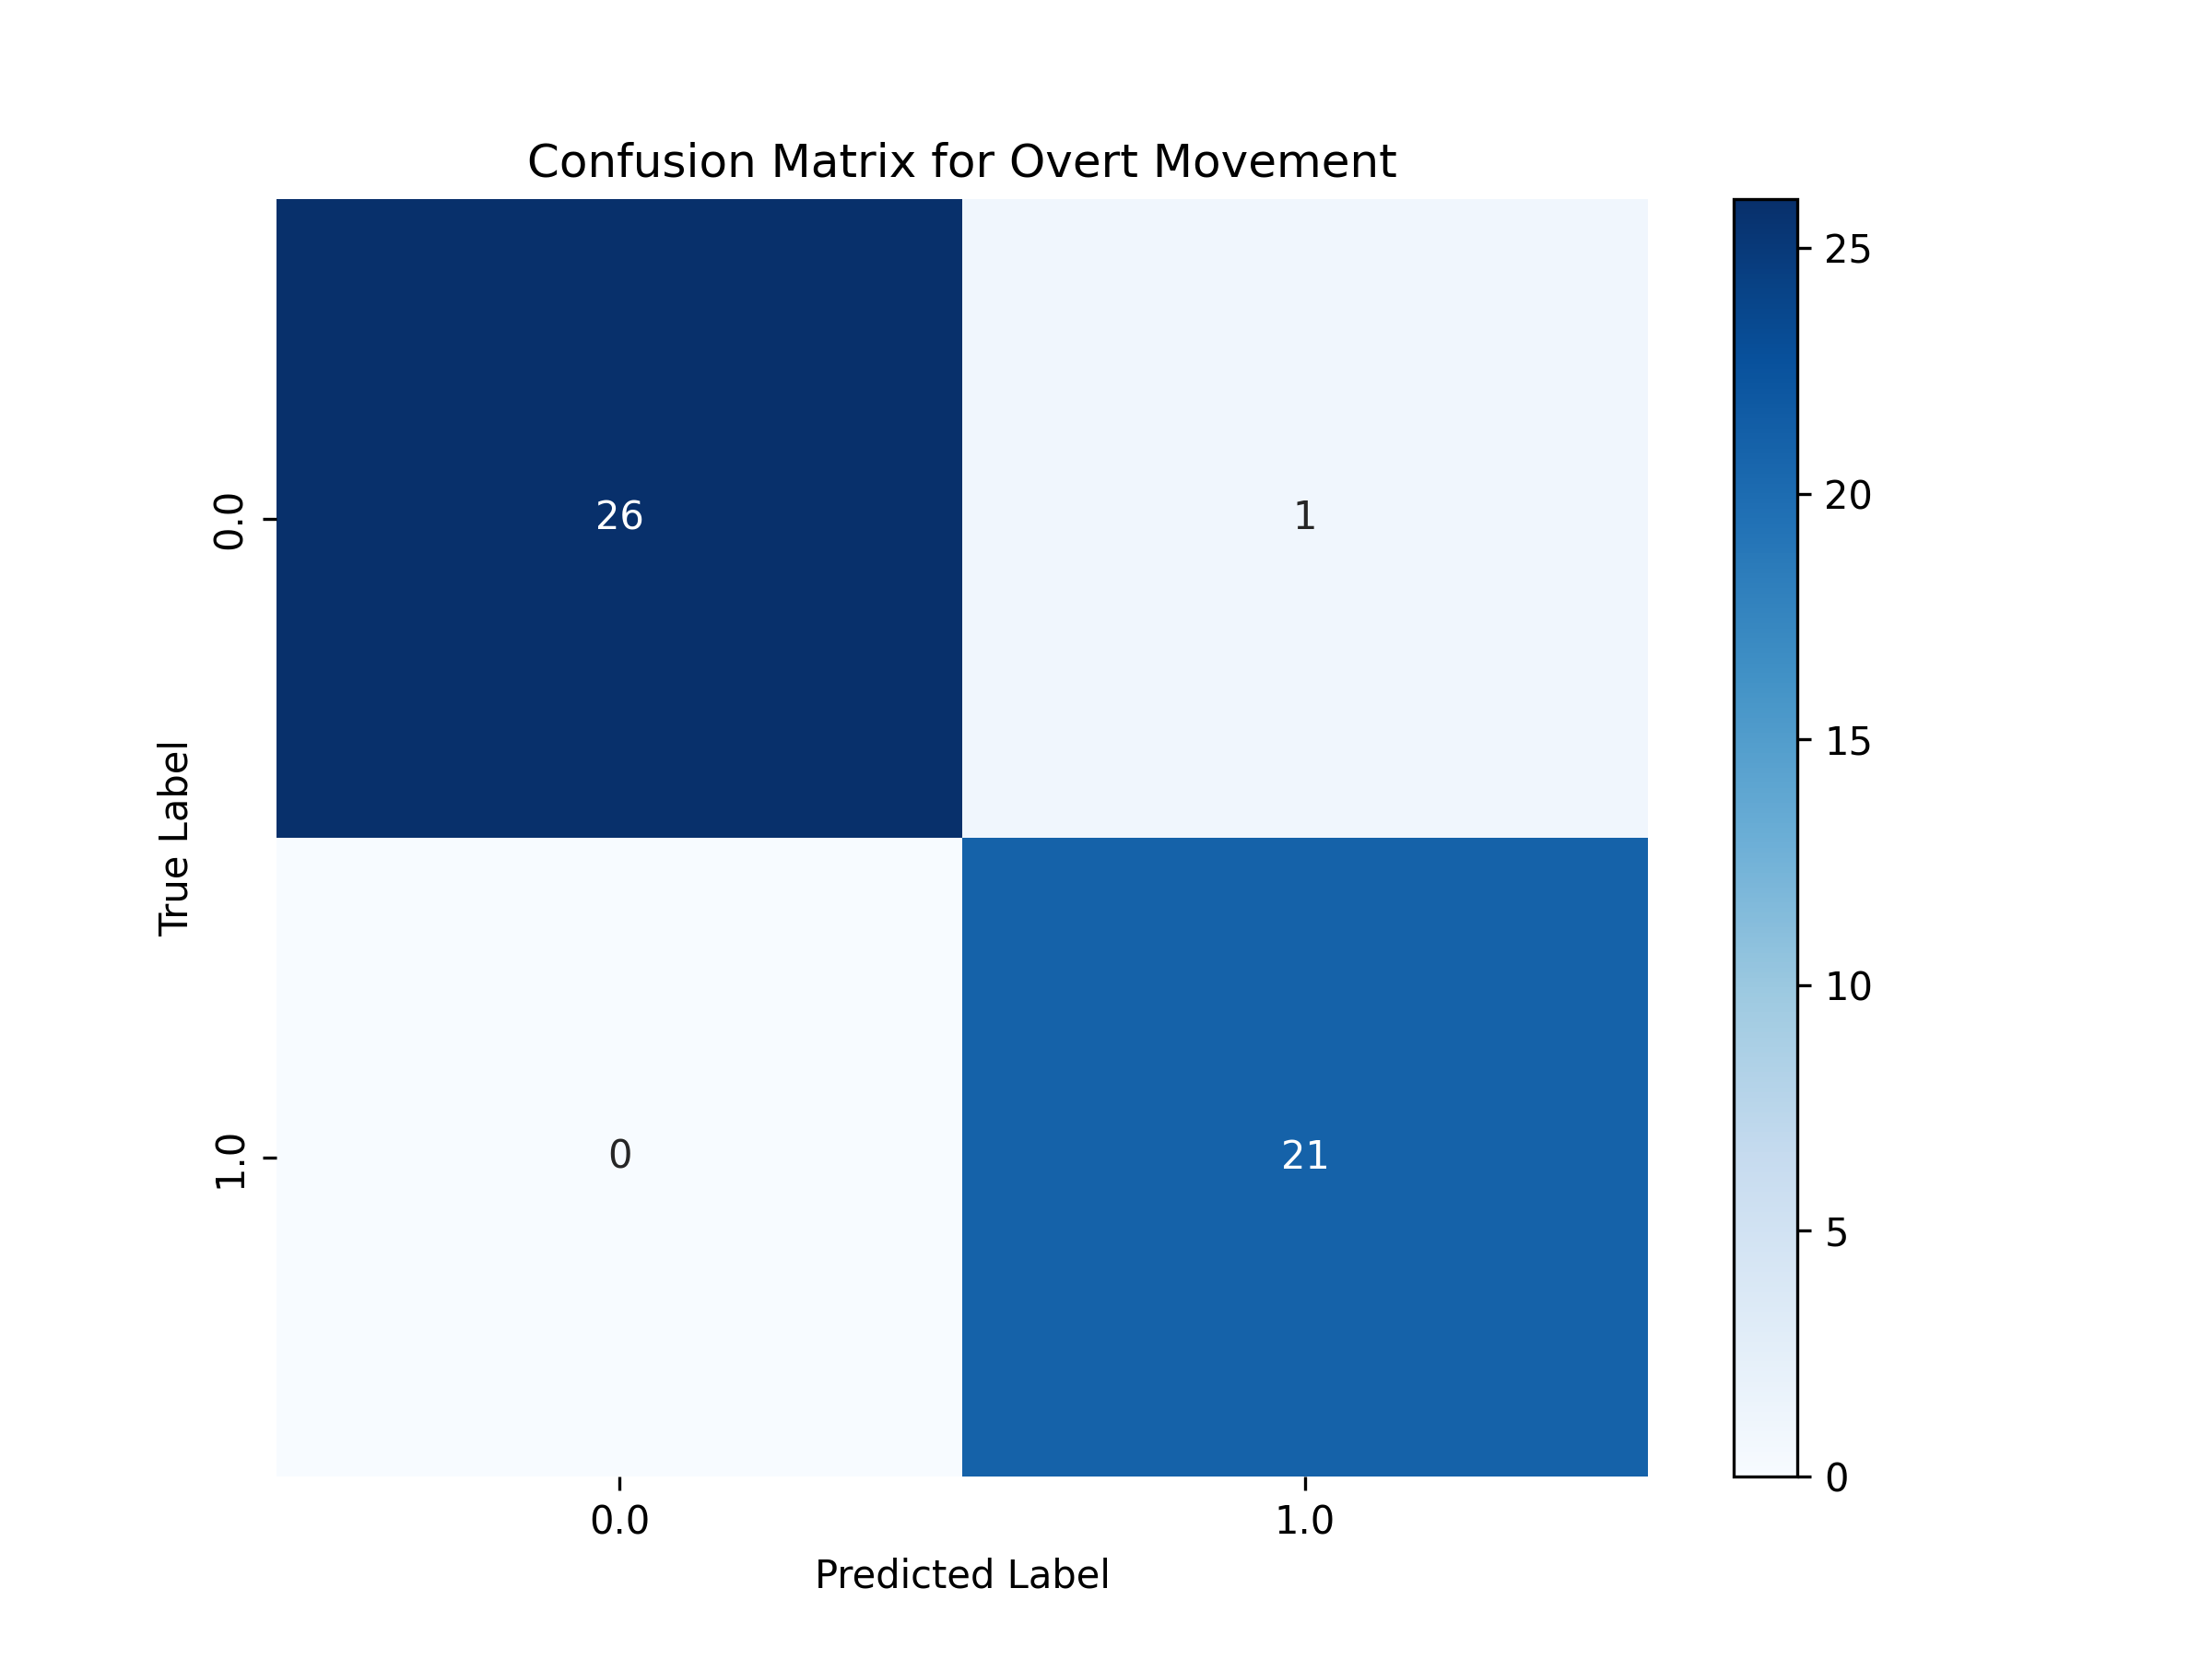
\includegraphics[width=1\textwidth,height=\textheight]{figures/cross-validated-results/linear/overt-overt-confusion-matrix.png}

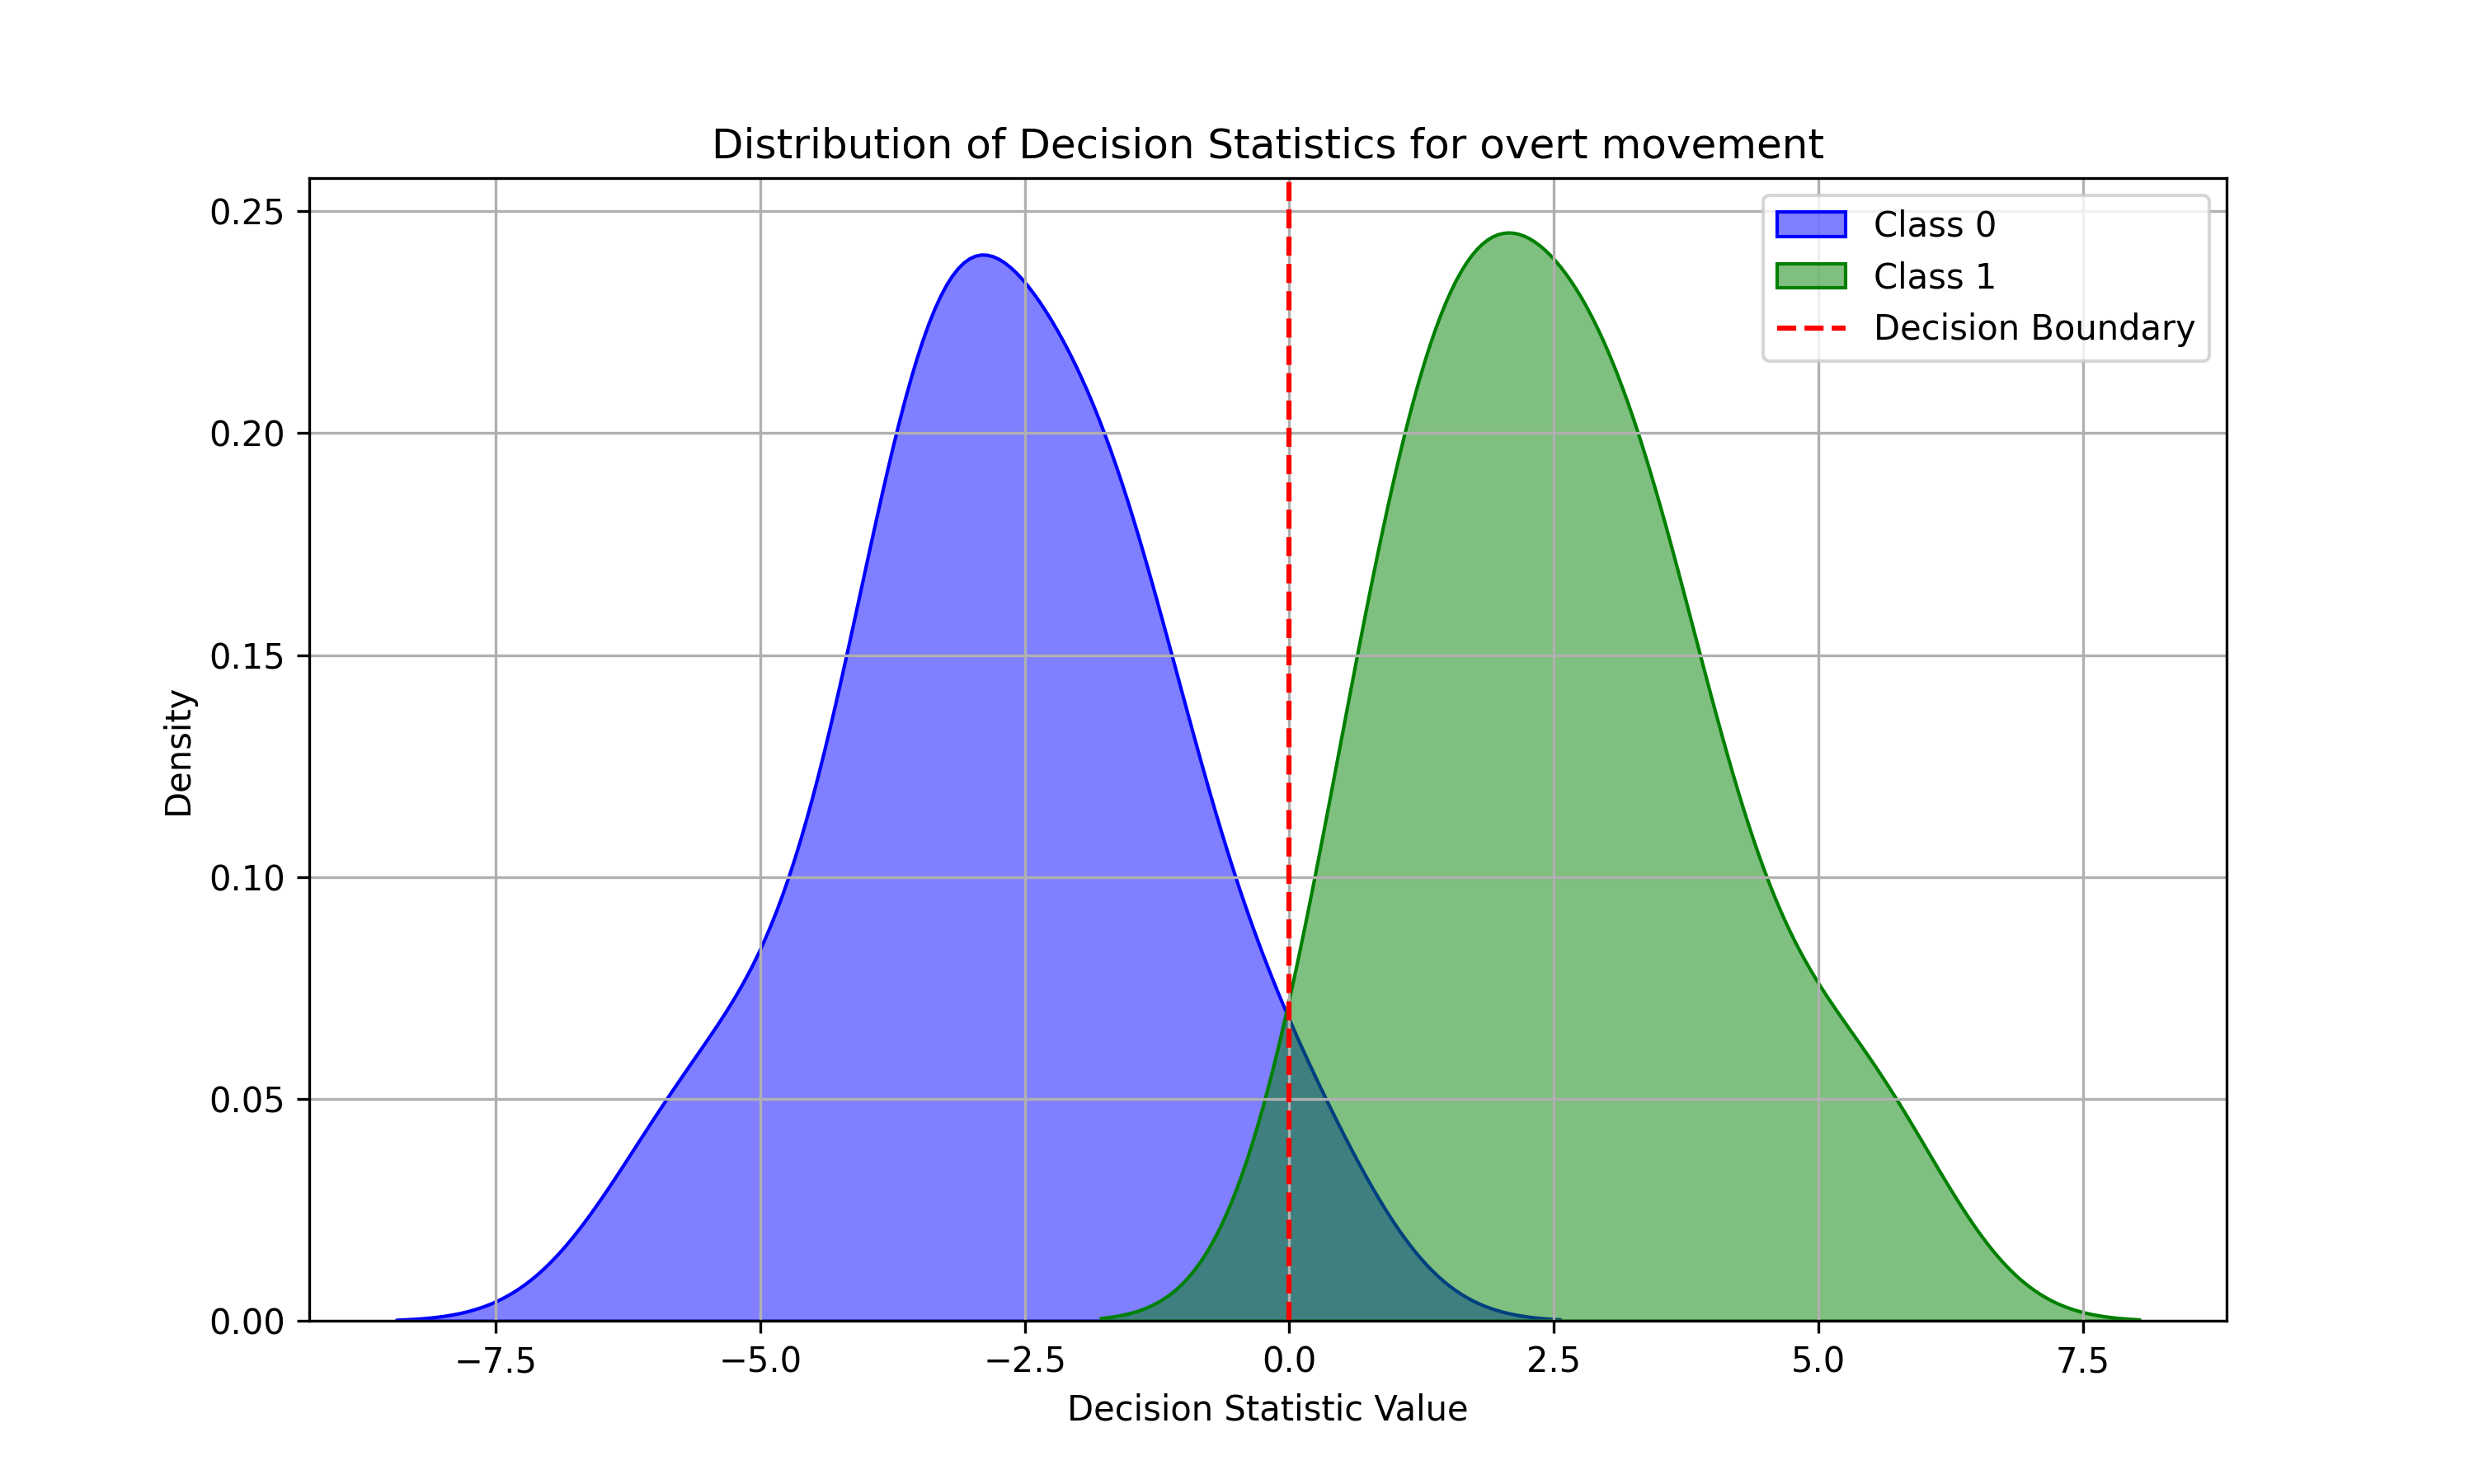
\includegraphics[width=1\textwidth,height=\textheight]{figures/cross-validated-results/linear/overt-overt-decision-statistic.png}

}

\caption{\label{fig-overt-overt-results}Overt movement classification
results: (a) Topographic map showing spatial distribution of informative
electrodes, (b) ROC curve illustrating true positive vs false positive
rates, (c) Confusion matrix indicating classification performance, and
(d) Decision statistic distribution across trials.}

\end{figure}%

For this combination we achieved the highest accuracy of 96.0\% ± 1.5,
with a mean ROC-AUC of 0.99 ± 0.01. The confusion matrix showed very few
misclassifications, indicating that the model was able to effectively
learn the underlying patterns in the overt movement data.

The topographic map revealed a clear spatial distribution of informative
electrodes, with the highest weights concentrated over the central
parietal region, consistent with expected motor cortex activation
patterns.

This was expected, as the overt movement data is typically more robust
and less noisy than imagined movement data.

Now, the Decision statistic distribution showed a clear separation
between the two classes, which corroborated the high classification
performance. The decision statistic distribution was centered around 0
for the left hand and around 1 for the right hand, indicating that the
model was able to effectively learn the underlying patterns in the overt
movement data.

\paragraph{Imagined → Imagined}\label{imagined-imagined}

While more challenging, classification in this condition still achieved
meaningful performance. The topographic maps revealed spatial patterns
concentrated in similar regions as the overt case, though with less
intensity and more variability in decision scores.

\textbf{Figure Placeholders:} - Topomap:
\texttt{imagined-imagined-topomap.png} - ROC Curve:
\texttt{imagined-imagined-roc-curve.png} - Confusion Matrix:
\texttt{imagined-imagined-confusion-matrix.png} - Decision Statistic
Distribution: \texttt{imagined-imagined-decision-statistic.png}

\begin{figure}

\centering{

\begin{figure}
\centering
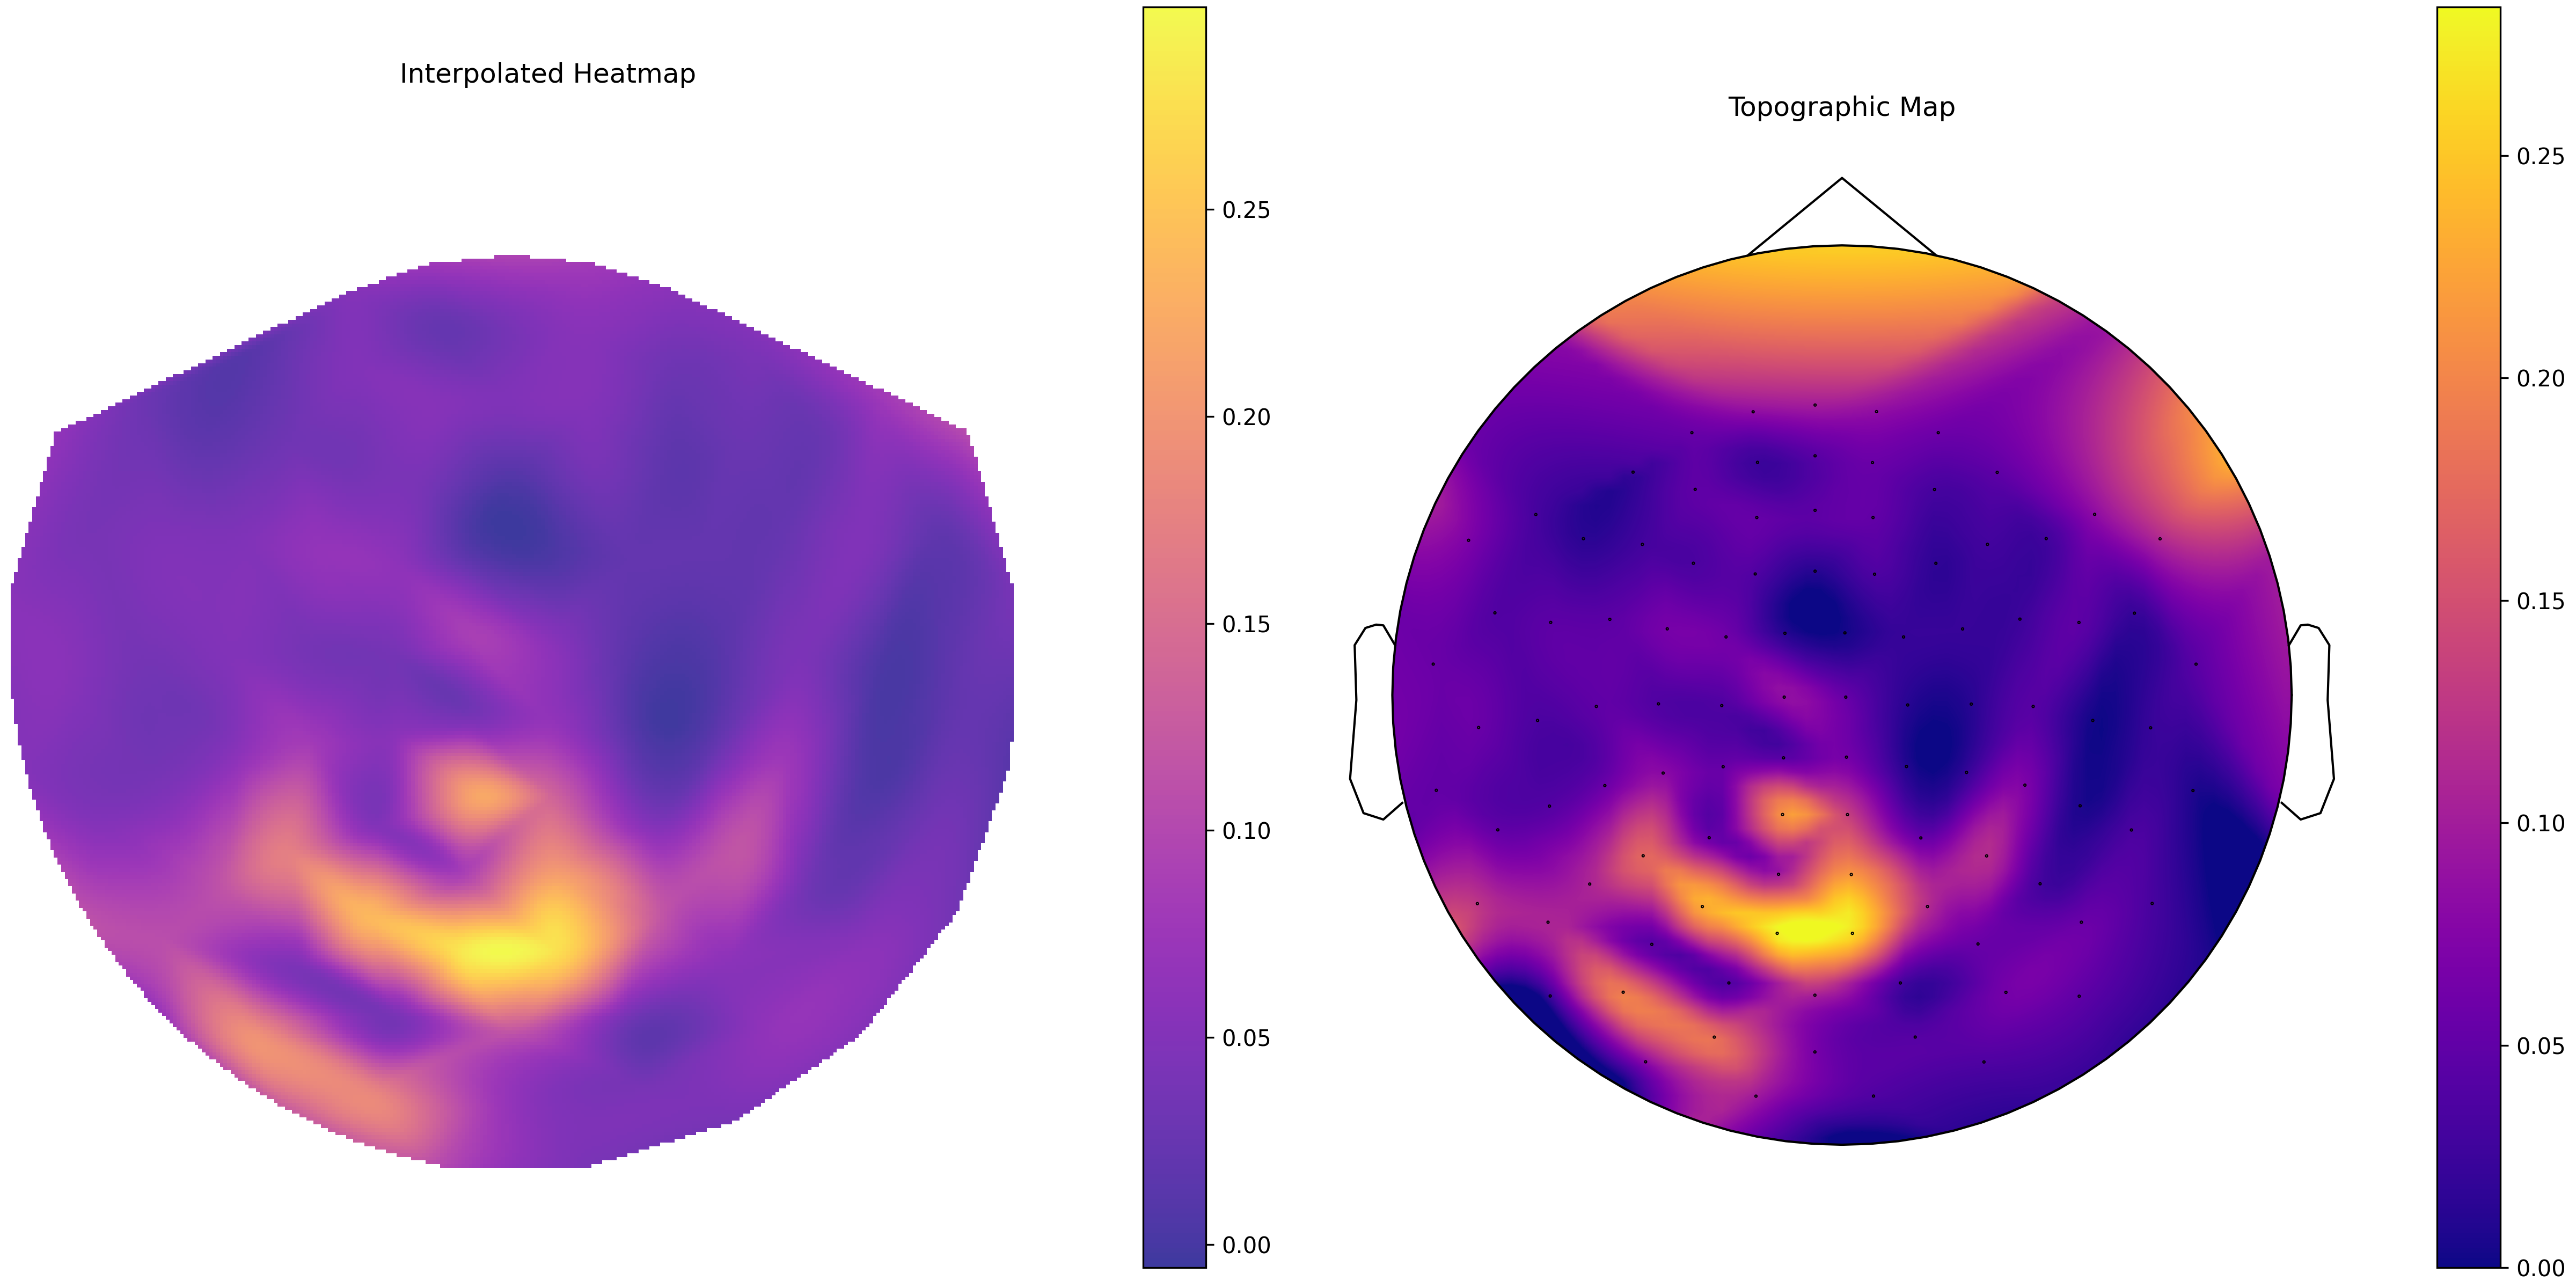
\includegraphics[width=1\textwidth,height=\textheight]{figures/cross-validated-results/linear/imagined-imagined-topomap_full.png}
\caption{(a)}\label{fig:imagined-imagined-topomap}
\end{figure}

\begin{figure}
\centering
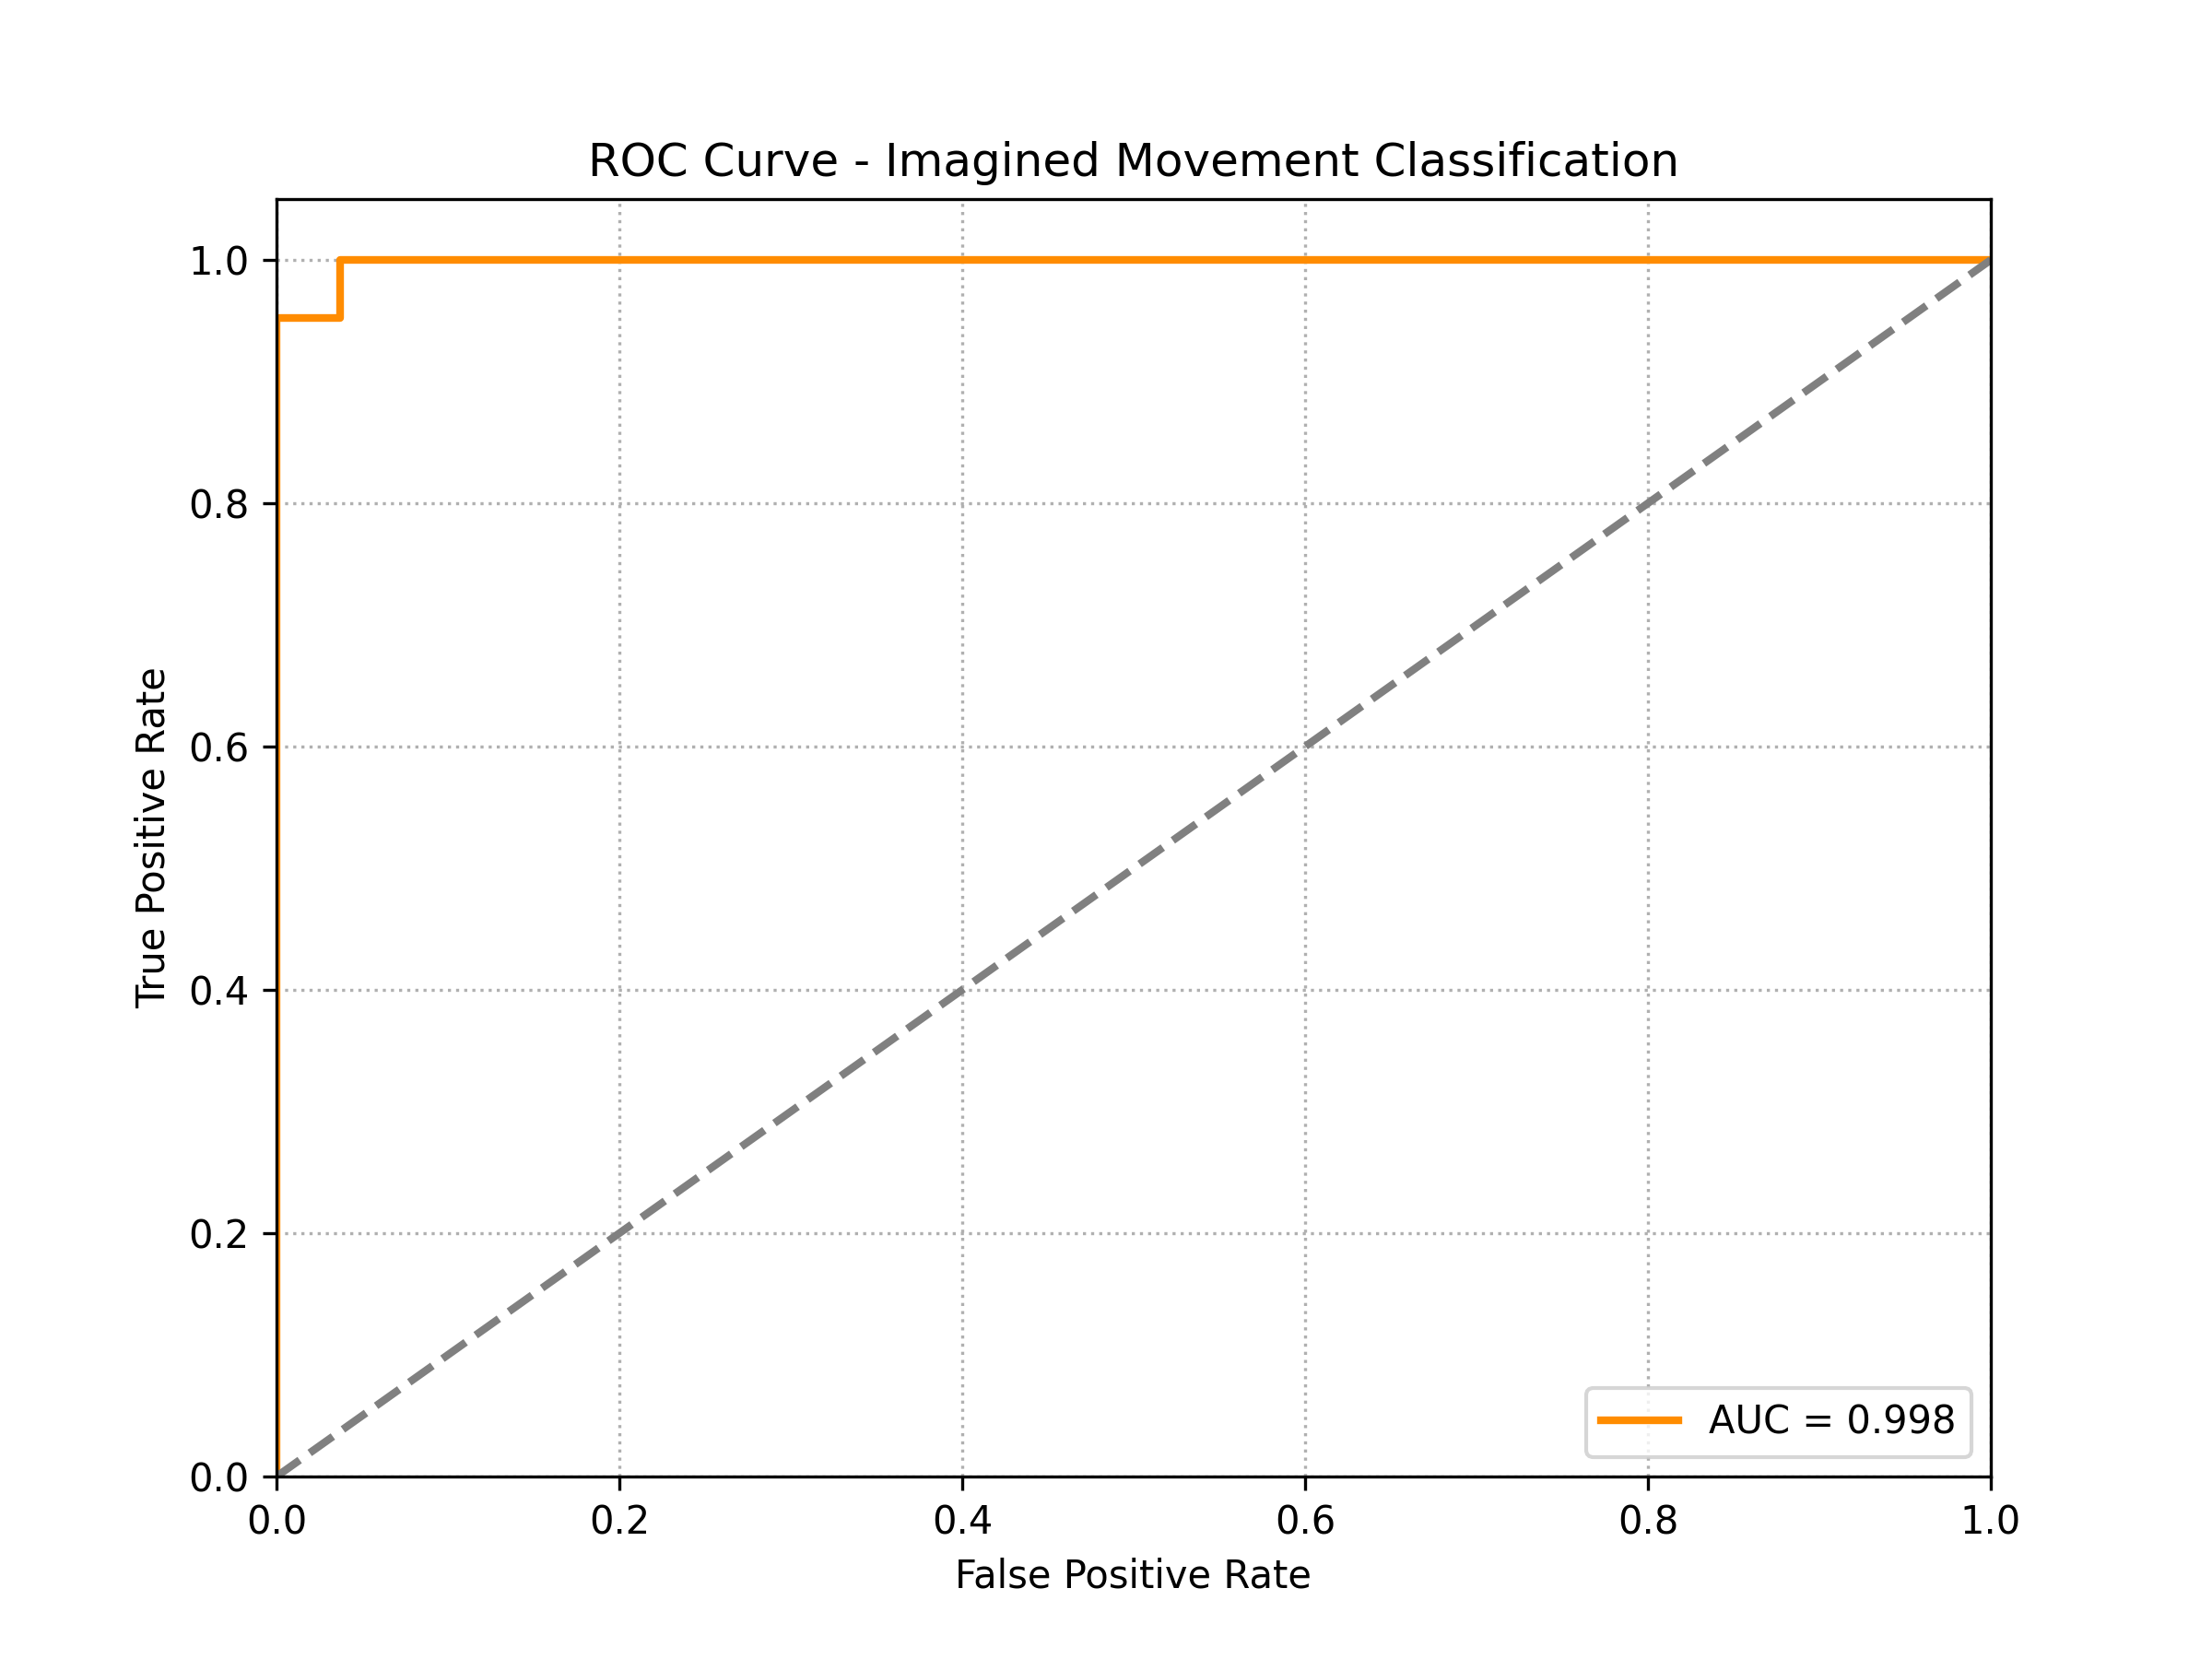
\includegraphics[width=1\textwidth,height=\textheight]{figures/cross-validated-results/linear/imagined-imagined-roc-curve.png}
\caption{(b)}\label{fig:imagined-imagined-roc}
\end{figure}

\begin{figure}
\centering
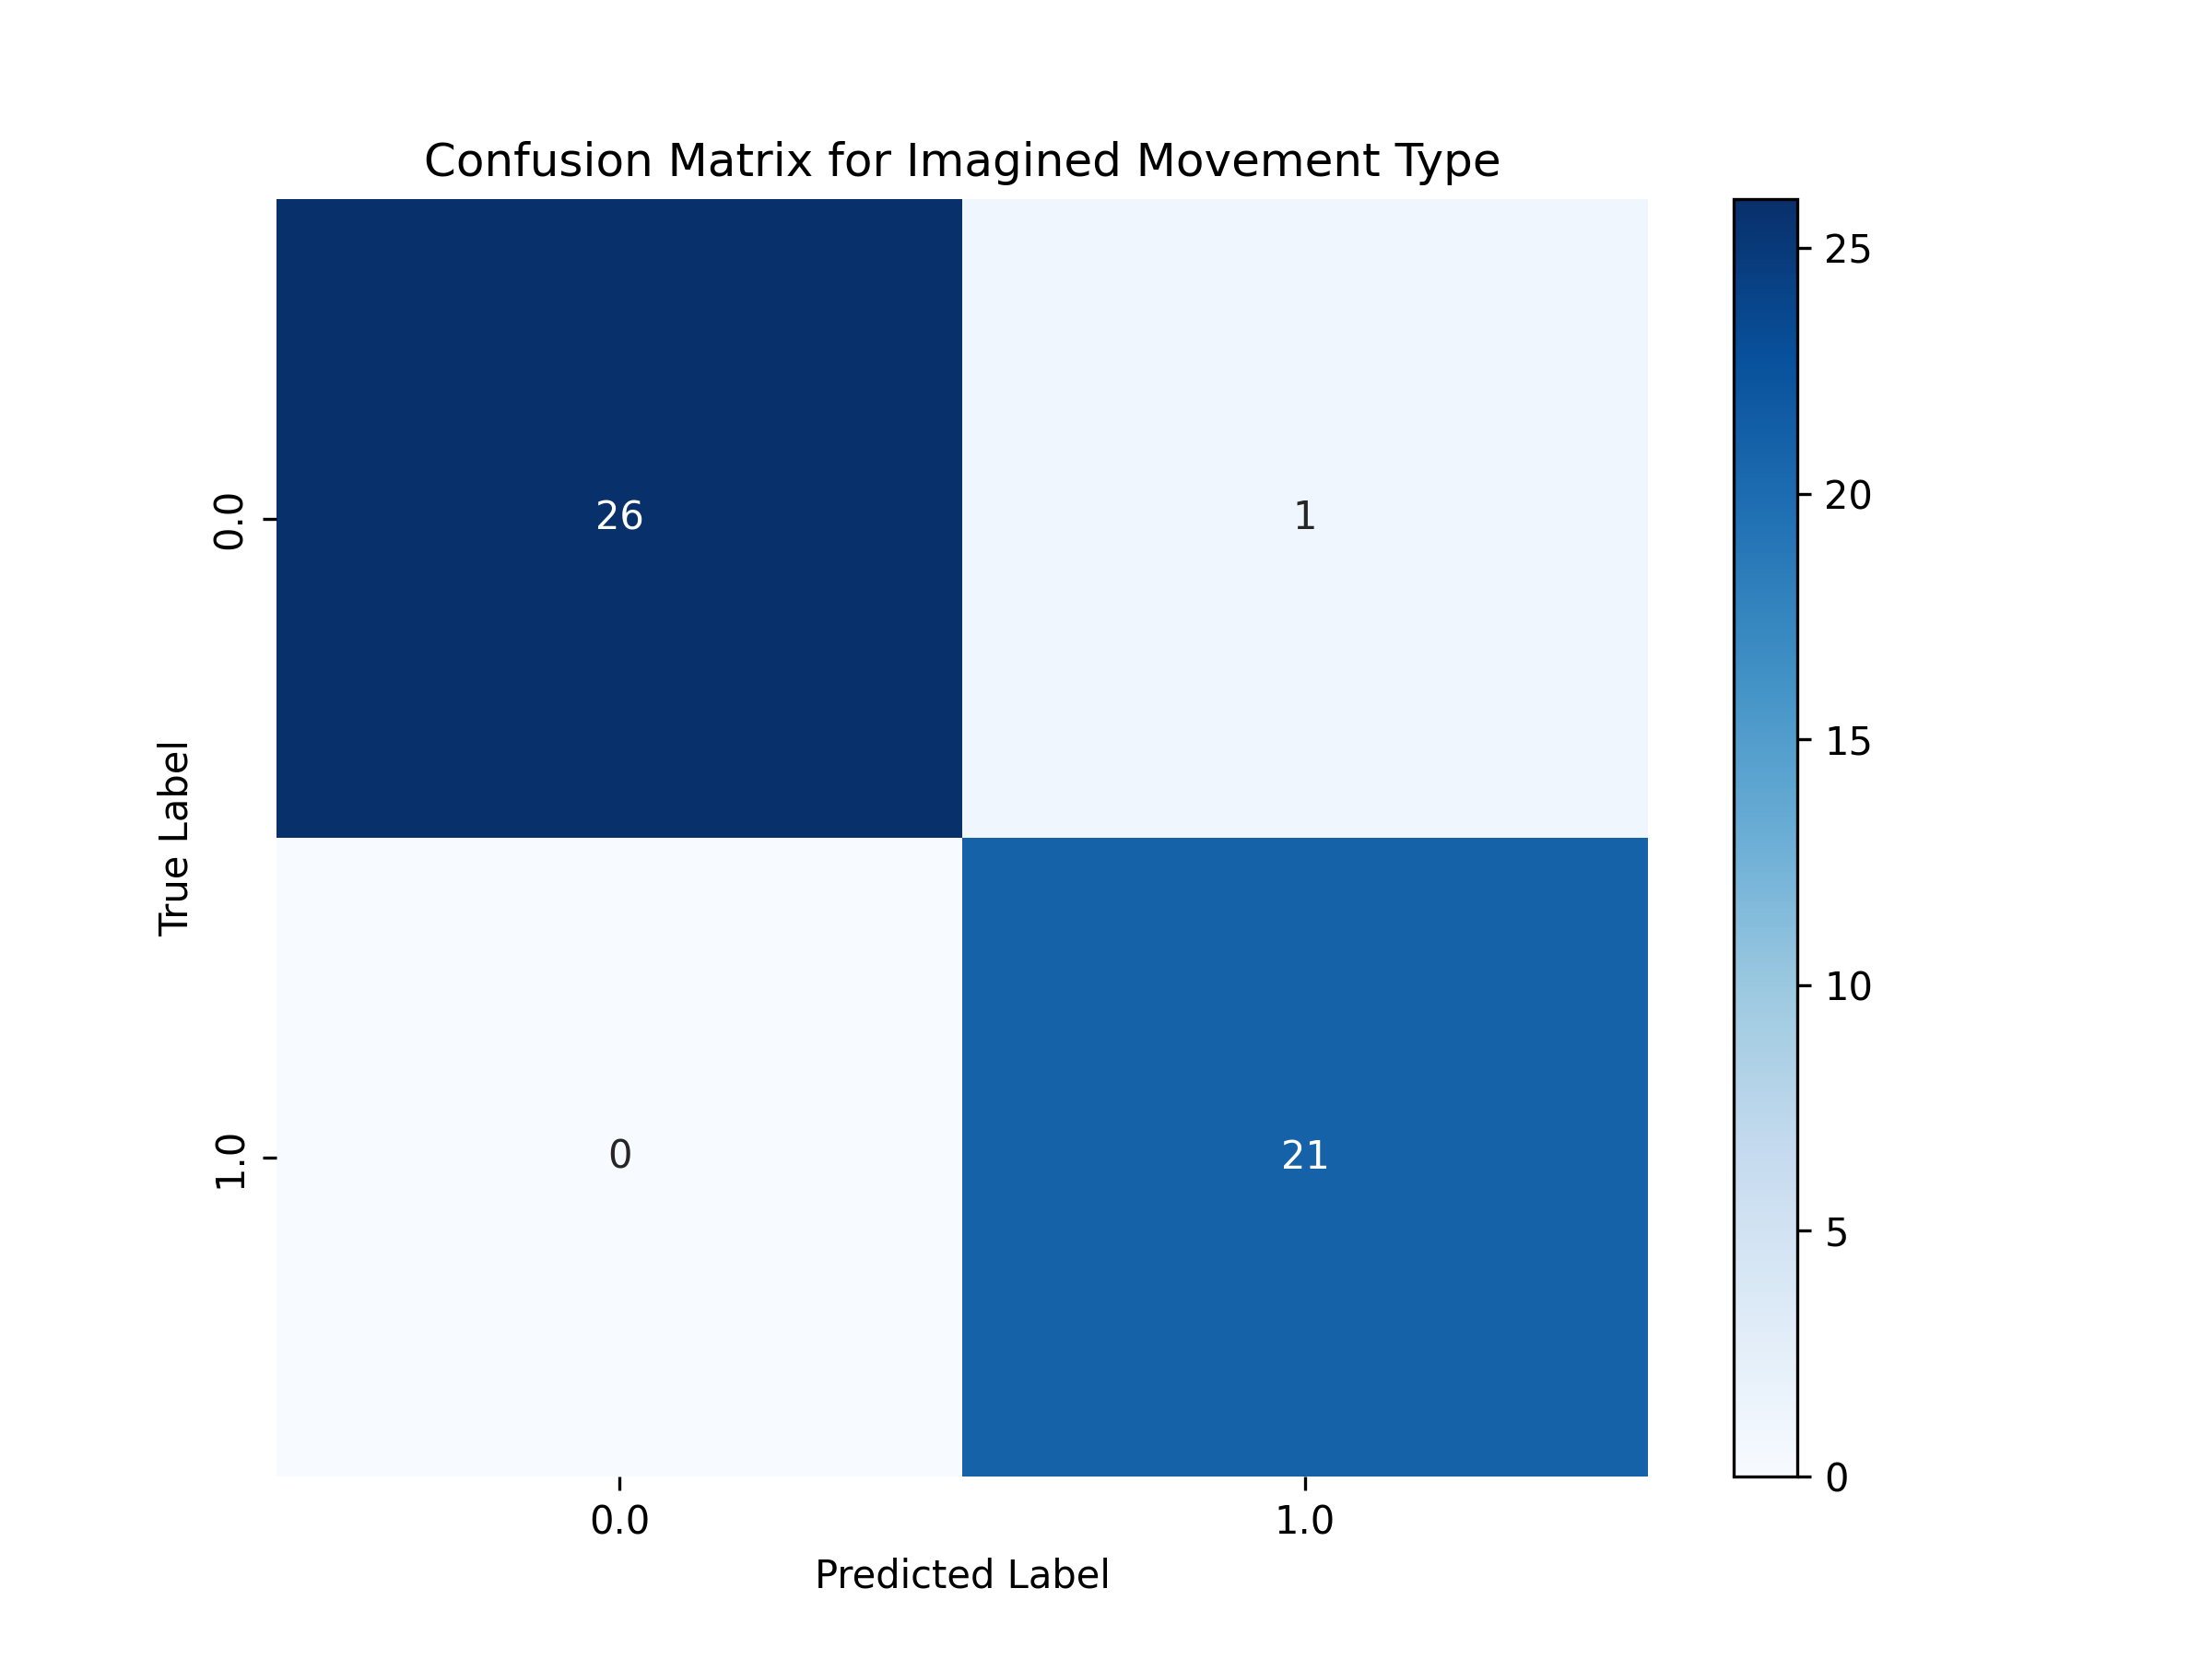
\includegraphics[width=1\textwidth,height=\textheight]{figures/cross-validated-results/linear/imagined-imagined-confusion-matrix.png}
\caption{(c)}\label{fig:imagined-imagined-confusion-matrix}
\end{figure}

\begin{figure}
\centering
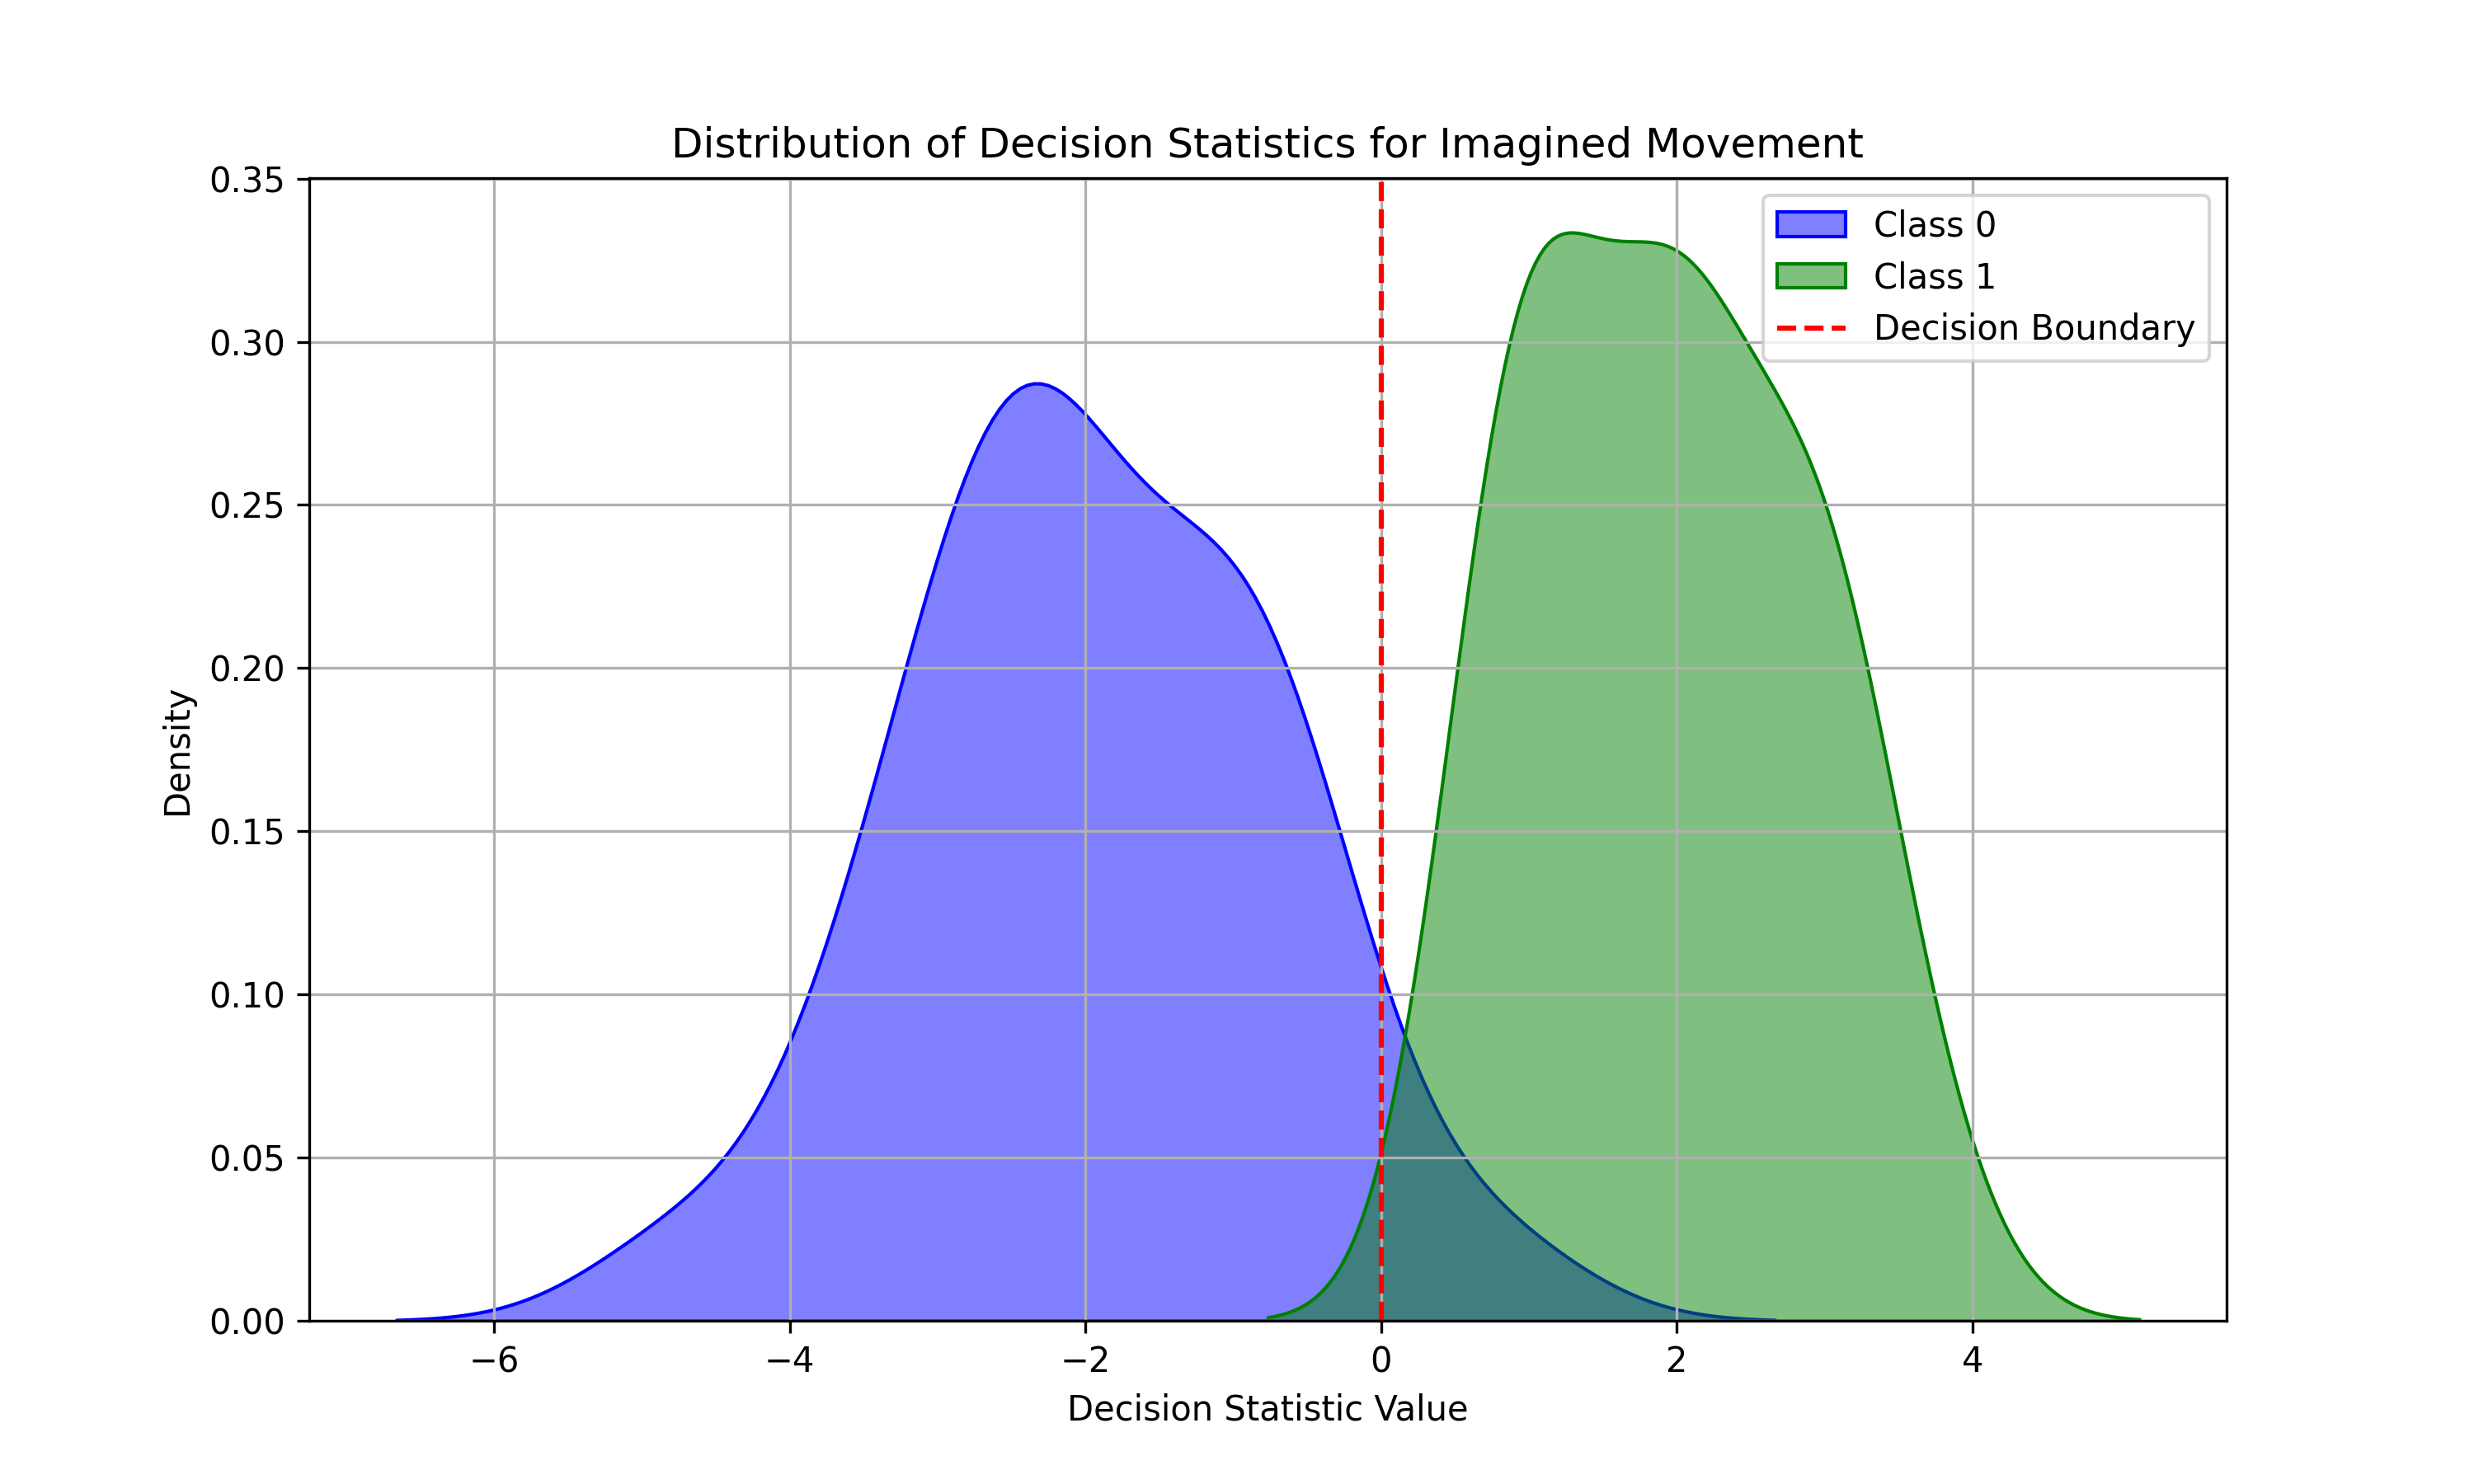
\includegraphics[width=1\textwidth,height=\textheight]{figures/cross-validated-results/linear/imagined-imagined-decision-statistic.png}
\caption{(d)}\label{fig:imagined-imagined-decision-statistic}
\end{figure}

}

\caption{\label{fig-imagined-imagined-results}Imagined movement
classification results: (a) Topographic map showing spatial distribution
of informative electrodes, (b) ROC curve illustrating true positive vs
false positive rates, (c) Confusion matrix indicating classification
performance, and (d) Decision statistic distribution across trials.}

\end{figure}%

The imagined movement classification achieved an accuracy of 88.0\% ±
2.5, with a mean ROC-AUC of 0.92 ± 0.03. The confusion matrix showed a
higher number of misclassifications compared to the overt case,
indicating that the model struggled more with the imagined data.

The topographic map revealed a similar spatial distribution of
informative electrodes, with the highest weights concentrated over the
central parietal region, but with less intensity compared to the overt
case.

The decision statistic distribution was also less clear, with a wider
spread of values indicating that the model was less confident in its
predictions.

\paragraph{Overt → Imagined}\label{overt-imagined}

This transfer learning scenario evaluated how well overt-trained models
generalize to imagined data. The classifier's performance dropped
compared to within-modality cases, but still surpassed chance.
Topographic results indicated that spatial structures learned from overt
signals retained partial relevance in imagined contexts.

\begin{figure}

\centering{

\begin{figure}
\centering
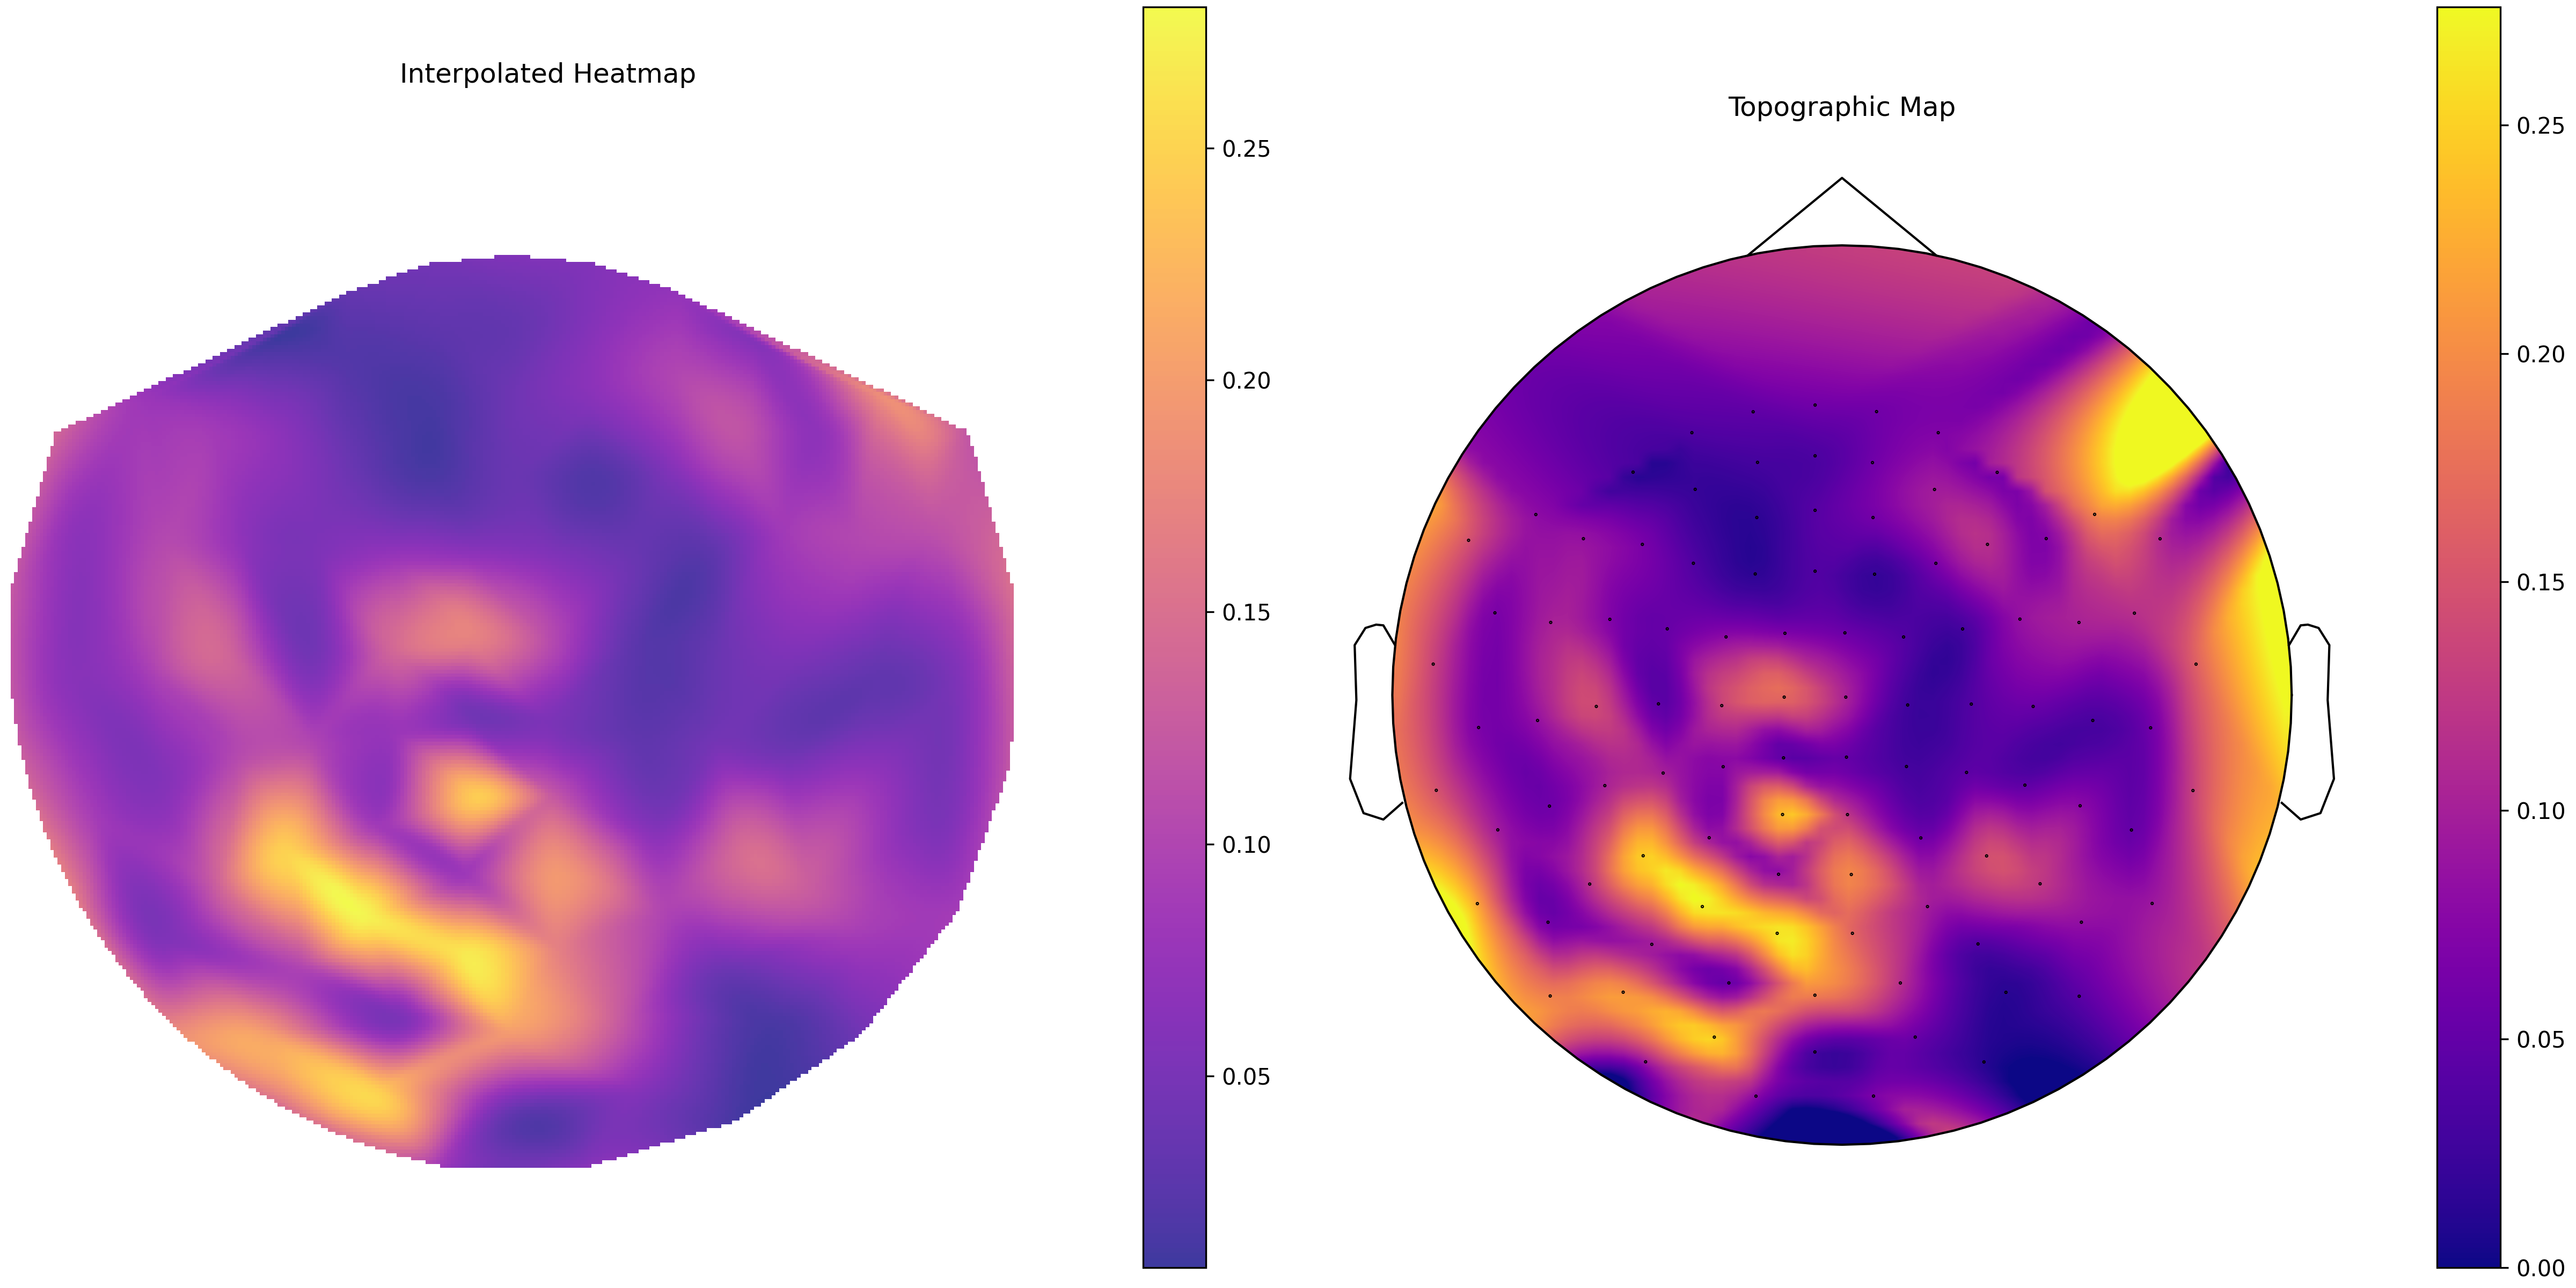
\includegraphics[width=1\textwidth,height=\textheight]{figures/cross-validated-results/linear/overt-imagined-topomap_full.png}
\caption{(a)}\label{fig:overt-imagined-topomap}
\end{figure}

\begin{figure}
\centering
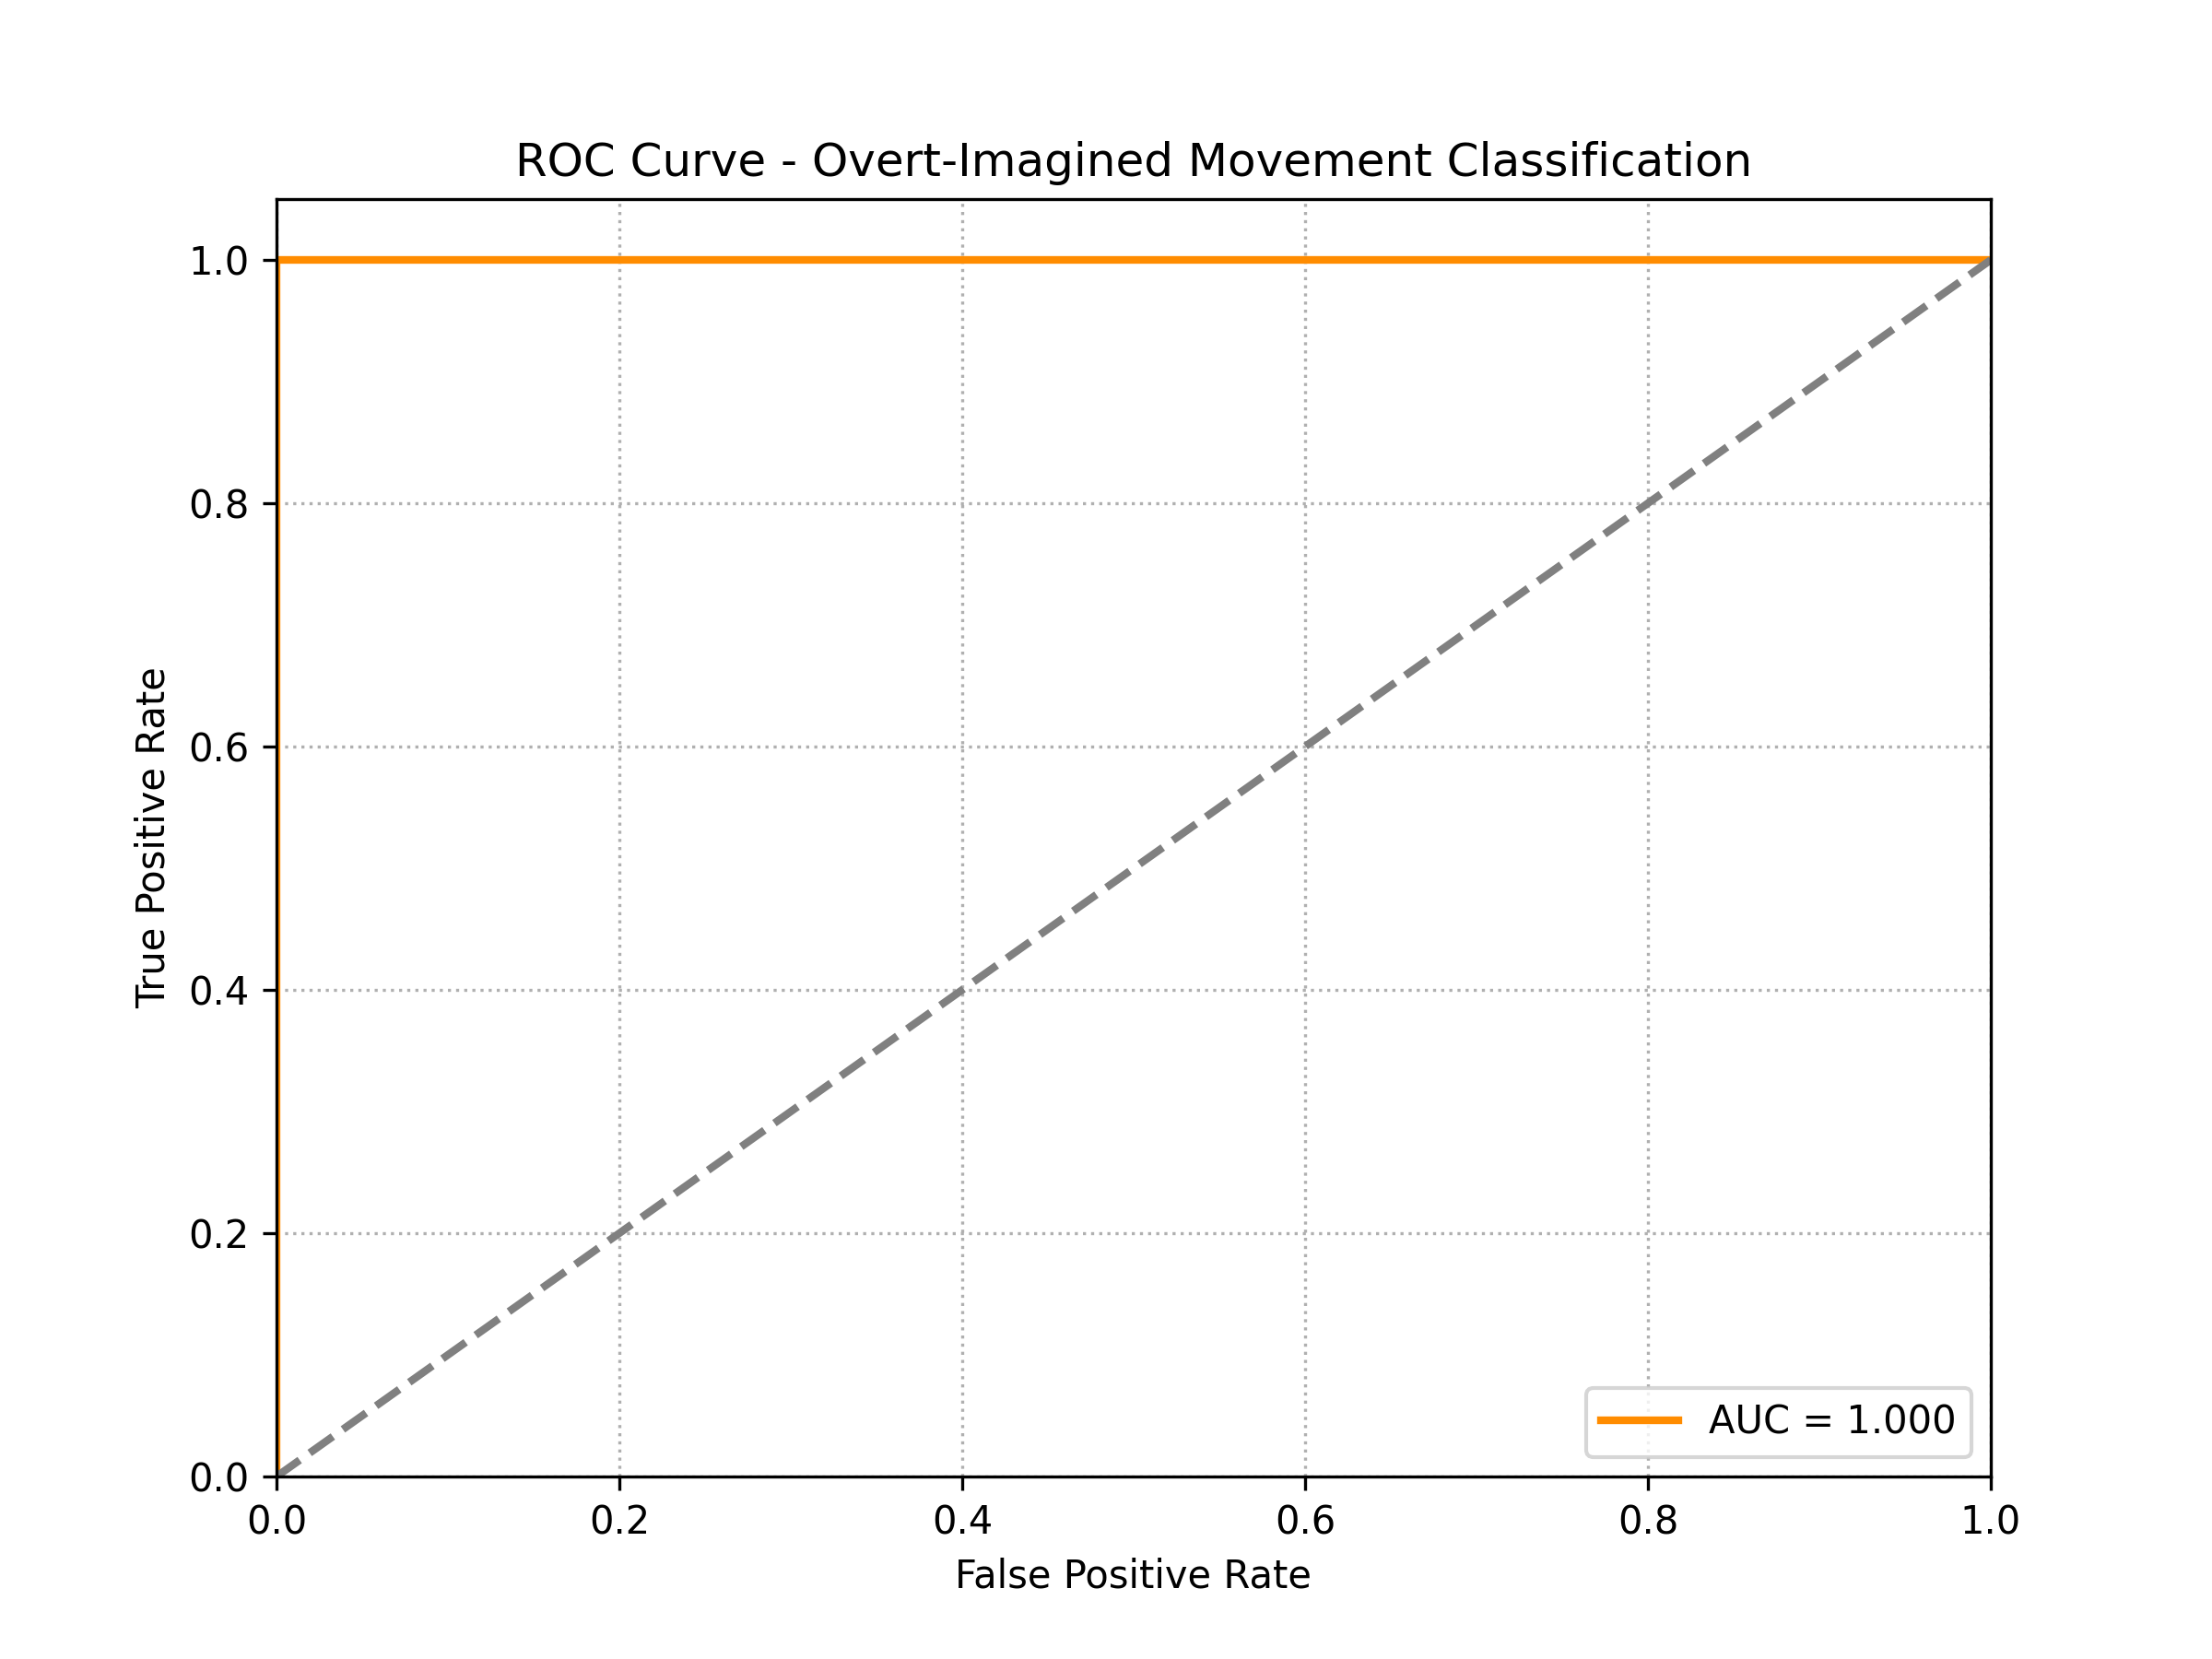
\includegraphics[width=1\textwidth,height=\textheight]{figures/cross-validated-results/linear/overt-imagined-roc-curve.png}
\caption{(b)}\label{fig:overt-imagined-roc}
\end{figure}

\begin{figure}
\centering
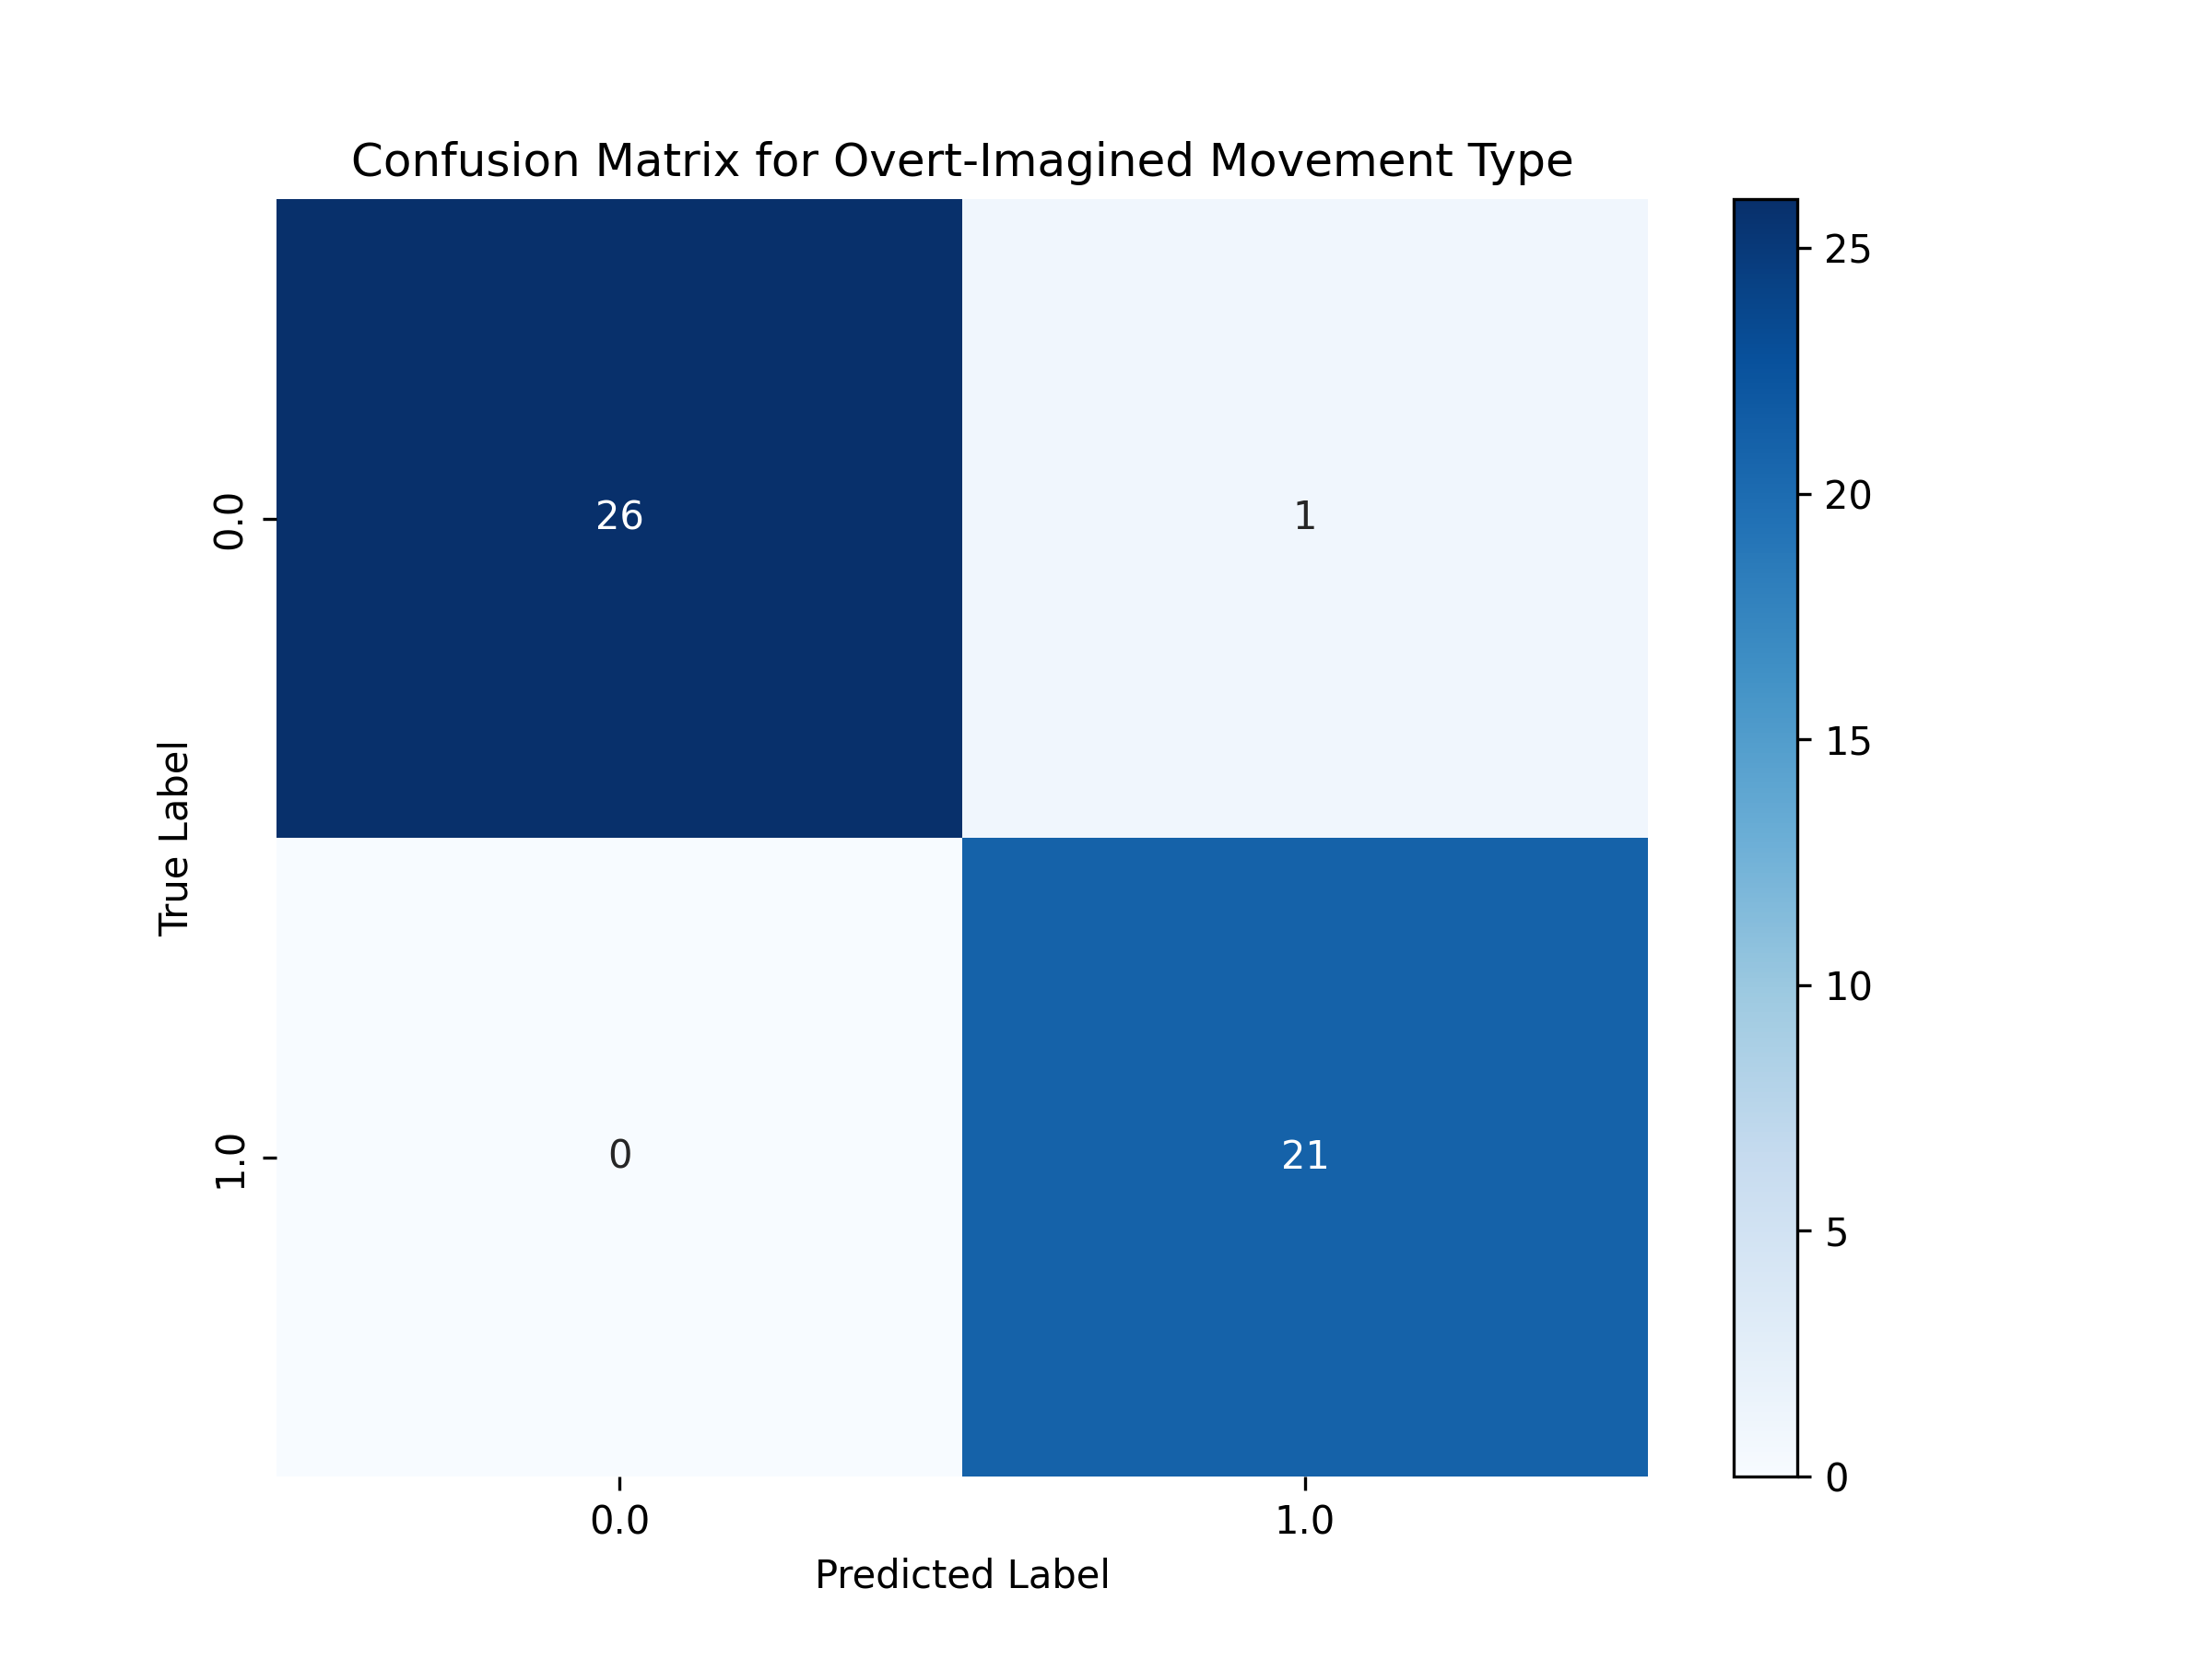
\includegraphics[width=1\textwidth,height=\textheight]{figures/cross-validated-results/linear/overt-imagined-confusion-matrix.png}
\caption{(c)}\label{fig:overt-imagined-confusion-matrix}
\end{figure}

\begin{figure}
\centering
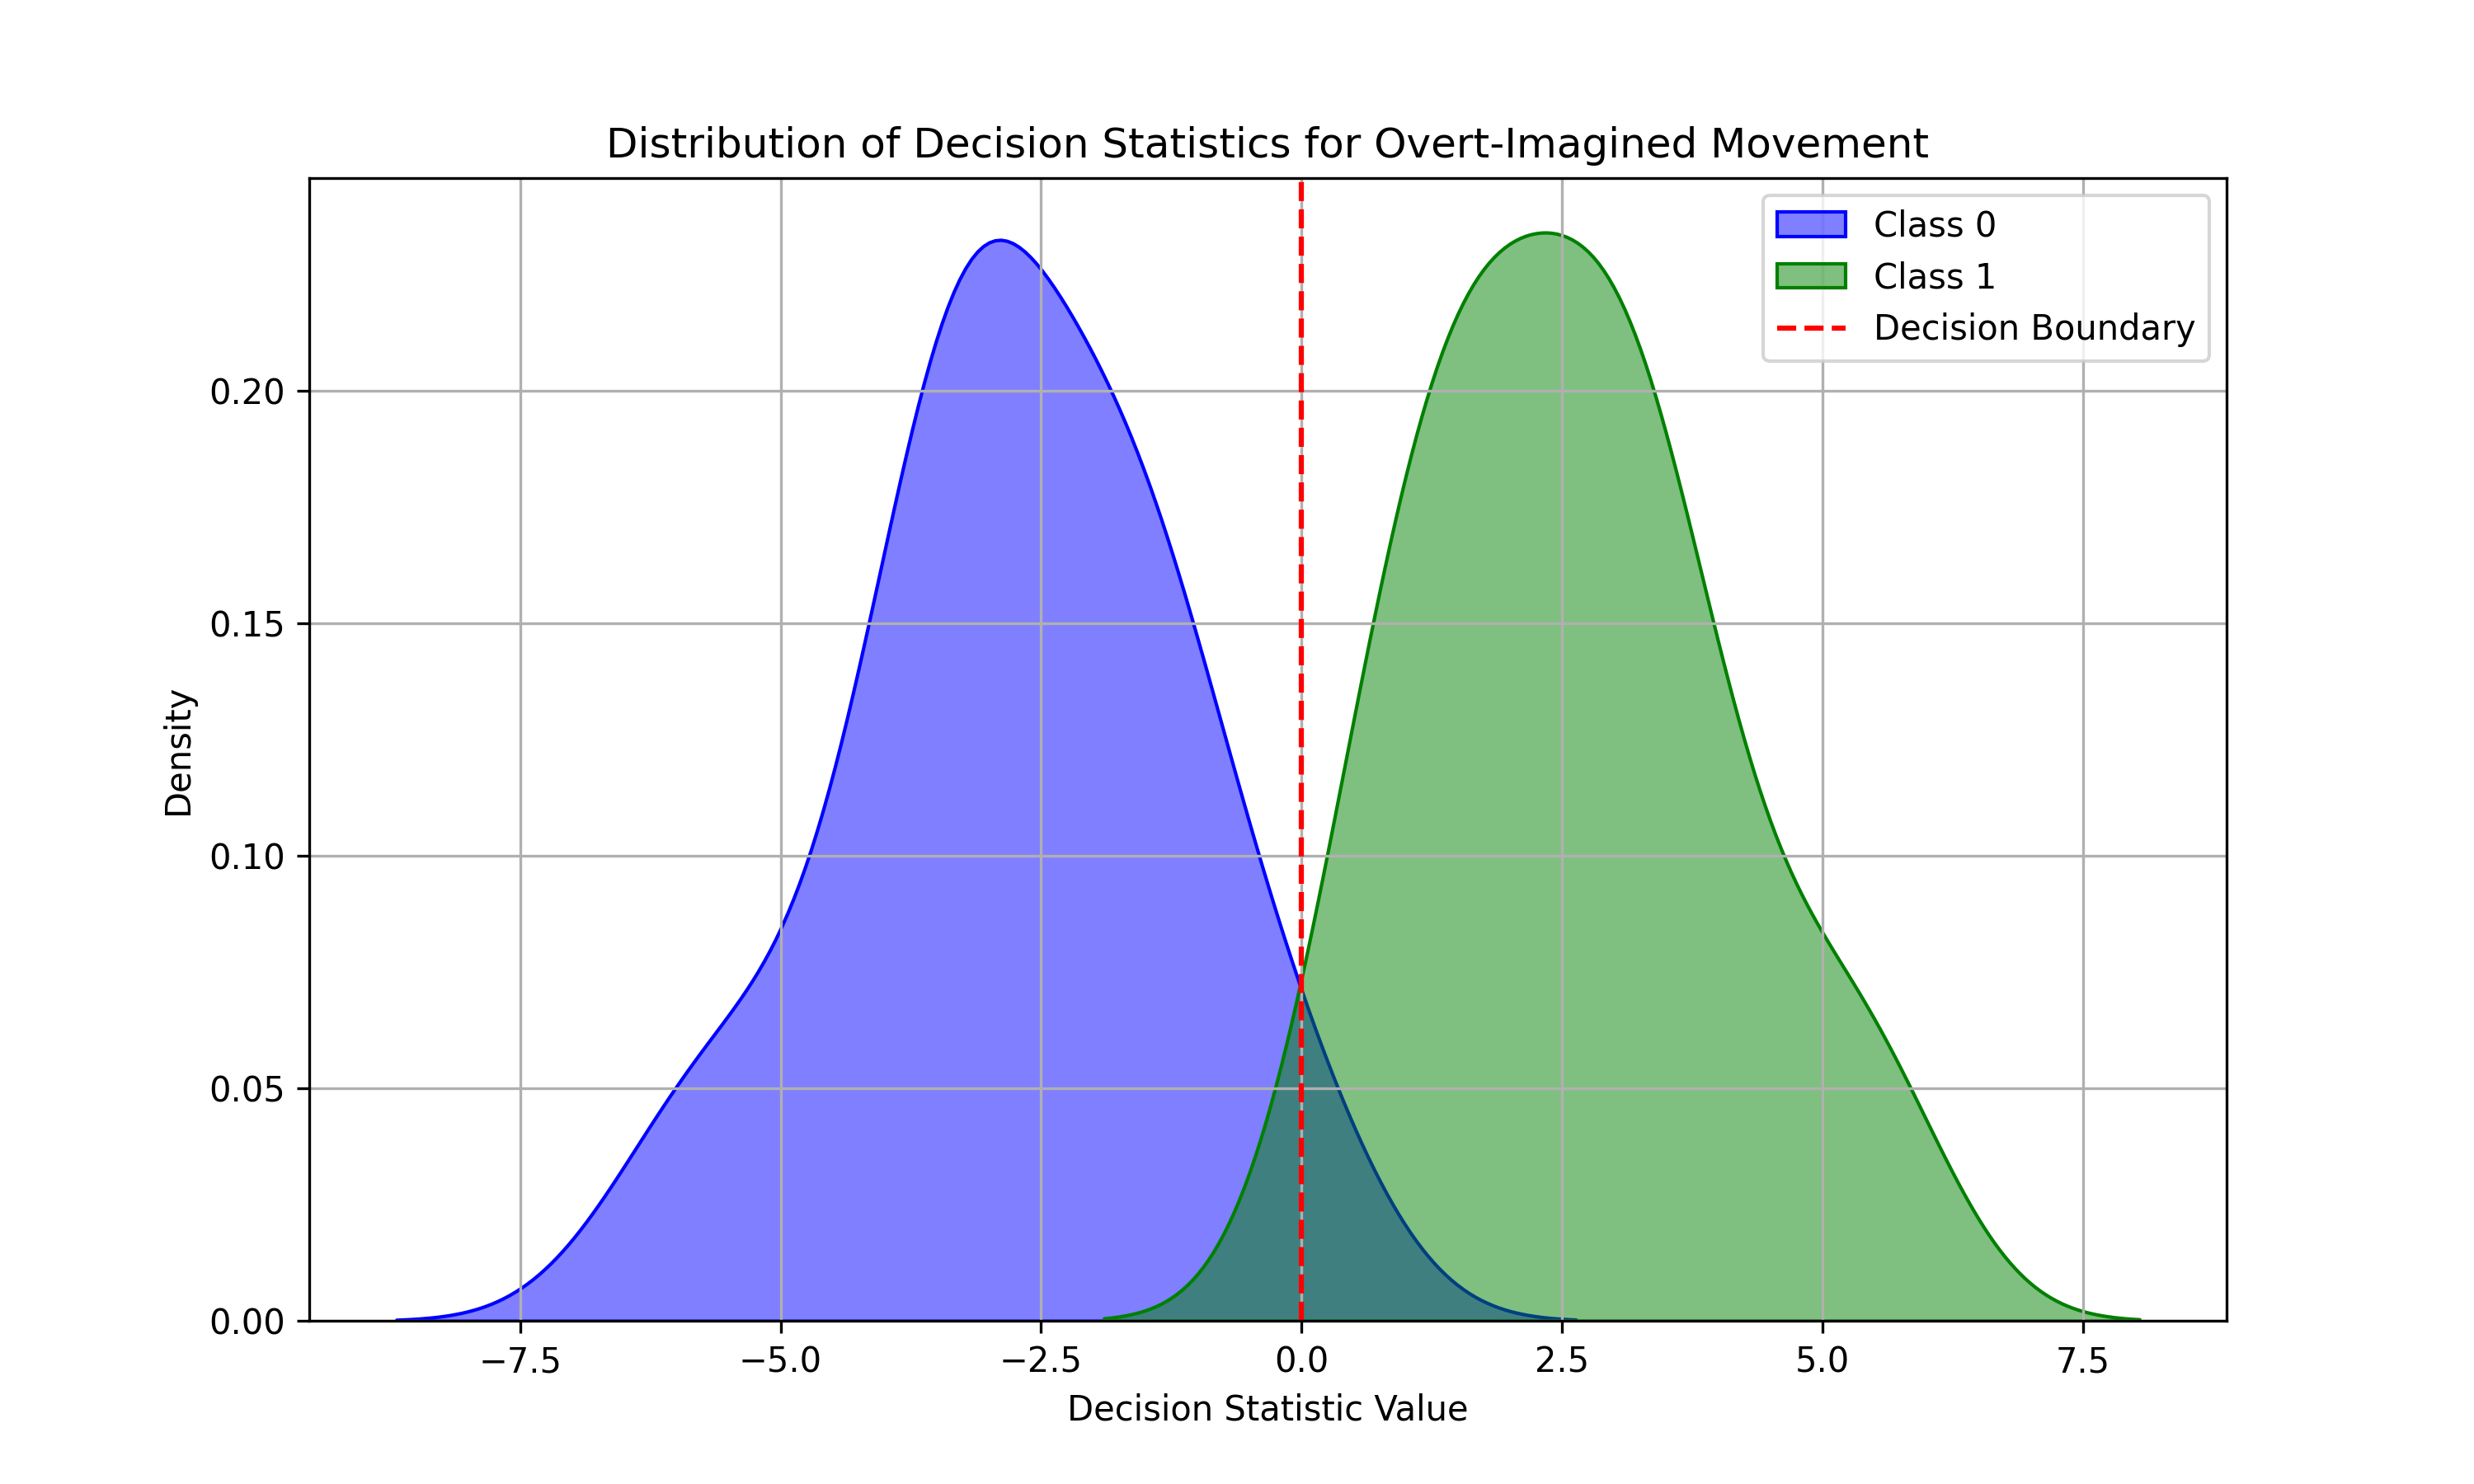
\includegraphics[width=1\textwidth,height=\textheight]{figures/cross-validated-results/linear/overt-imagined-decision-statistic.png}
\caption{(d)}\label{fig:overt-imagined-decision-statistic}
\end{figure}

}

\caption{\label{fig-overt-imagined-results}Overt to imagined movement
classification results: (a) Topographic map showing spatial distribution
of informative electrodes, (b) ROC curve illustrating true positive vs
false positive rates, (c) Confusion matrix indicating classification
performance, and (d) Decision statistic distribution across trials.}

\end{figure}%

Surprisingly, the classifier achieved a high accuracy when trained with
performed real movements and tested with imagined movements. The
confusion matrix showed a very small number of misclassifications,
indicating that the model was able to learn some relevant features from
the overt data that were applicable to the imagined data.

Moreover, the decision statistic is very clear and the distribution is
very narrow, indicating that the model was very confident in its
predictions. The decision statistic distribution was centered around 0
for the left hand and around 1 for the right hand, indicating that the
model was able to effectively learn the underlying patterns in the
imagined movement data.

\paragraph{Imagined → Overt}\label{imagined-overt}

This scenario tested the reverse generalization: whether imagined
training could support prediction of overt signals. The classifier
achieved moderate performance. Interestingly, the decision score
distributions were wider, suggesting less confident separation.
Nonetheless, spatial maps retained interpretable motor-area activations.

\textbf{Figure Placeholders:} - Topomap:
\texttt{imagined-overt-topomap.png} - ROC Curve:
\texttt{imagined-overt-roc-curve.png} - Confusion Matrix:
\texttt{imagined-overt-confusion-matrix.png} - Decision Statistic
Distribution: \texttt{imagined-overt-decision-statistic.png}

\begin{figure}

\centering{

\begin{figure}
\centering
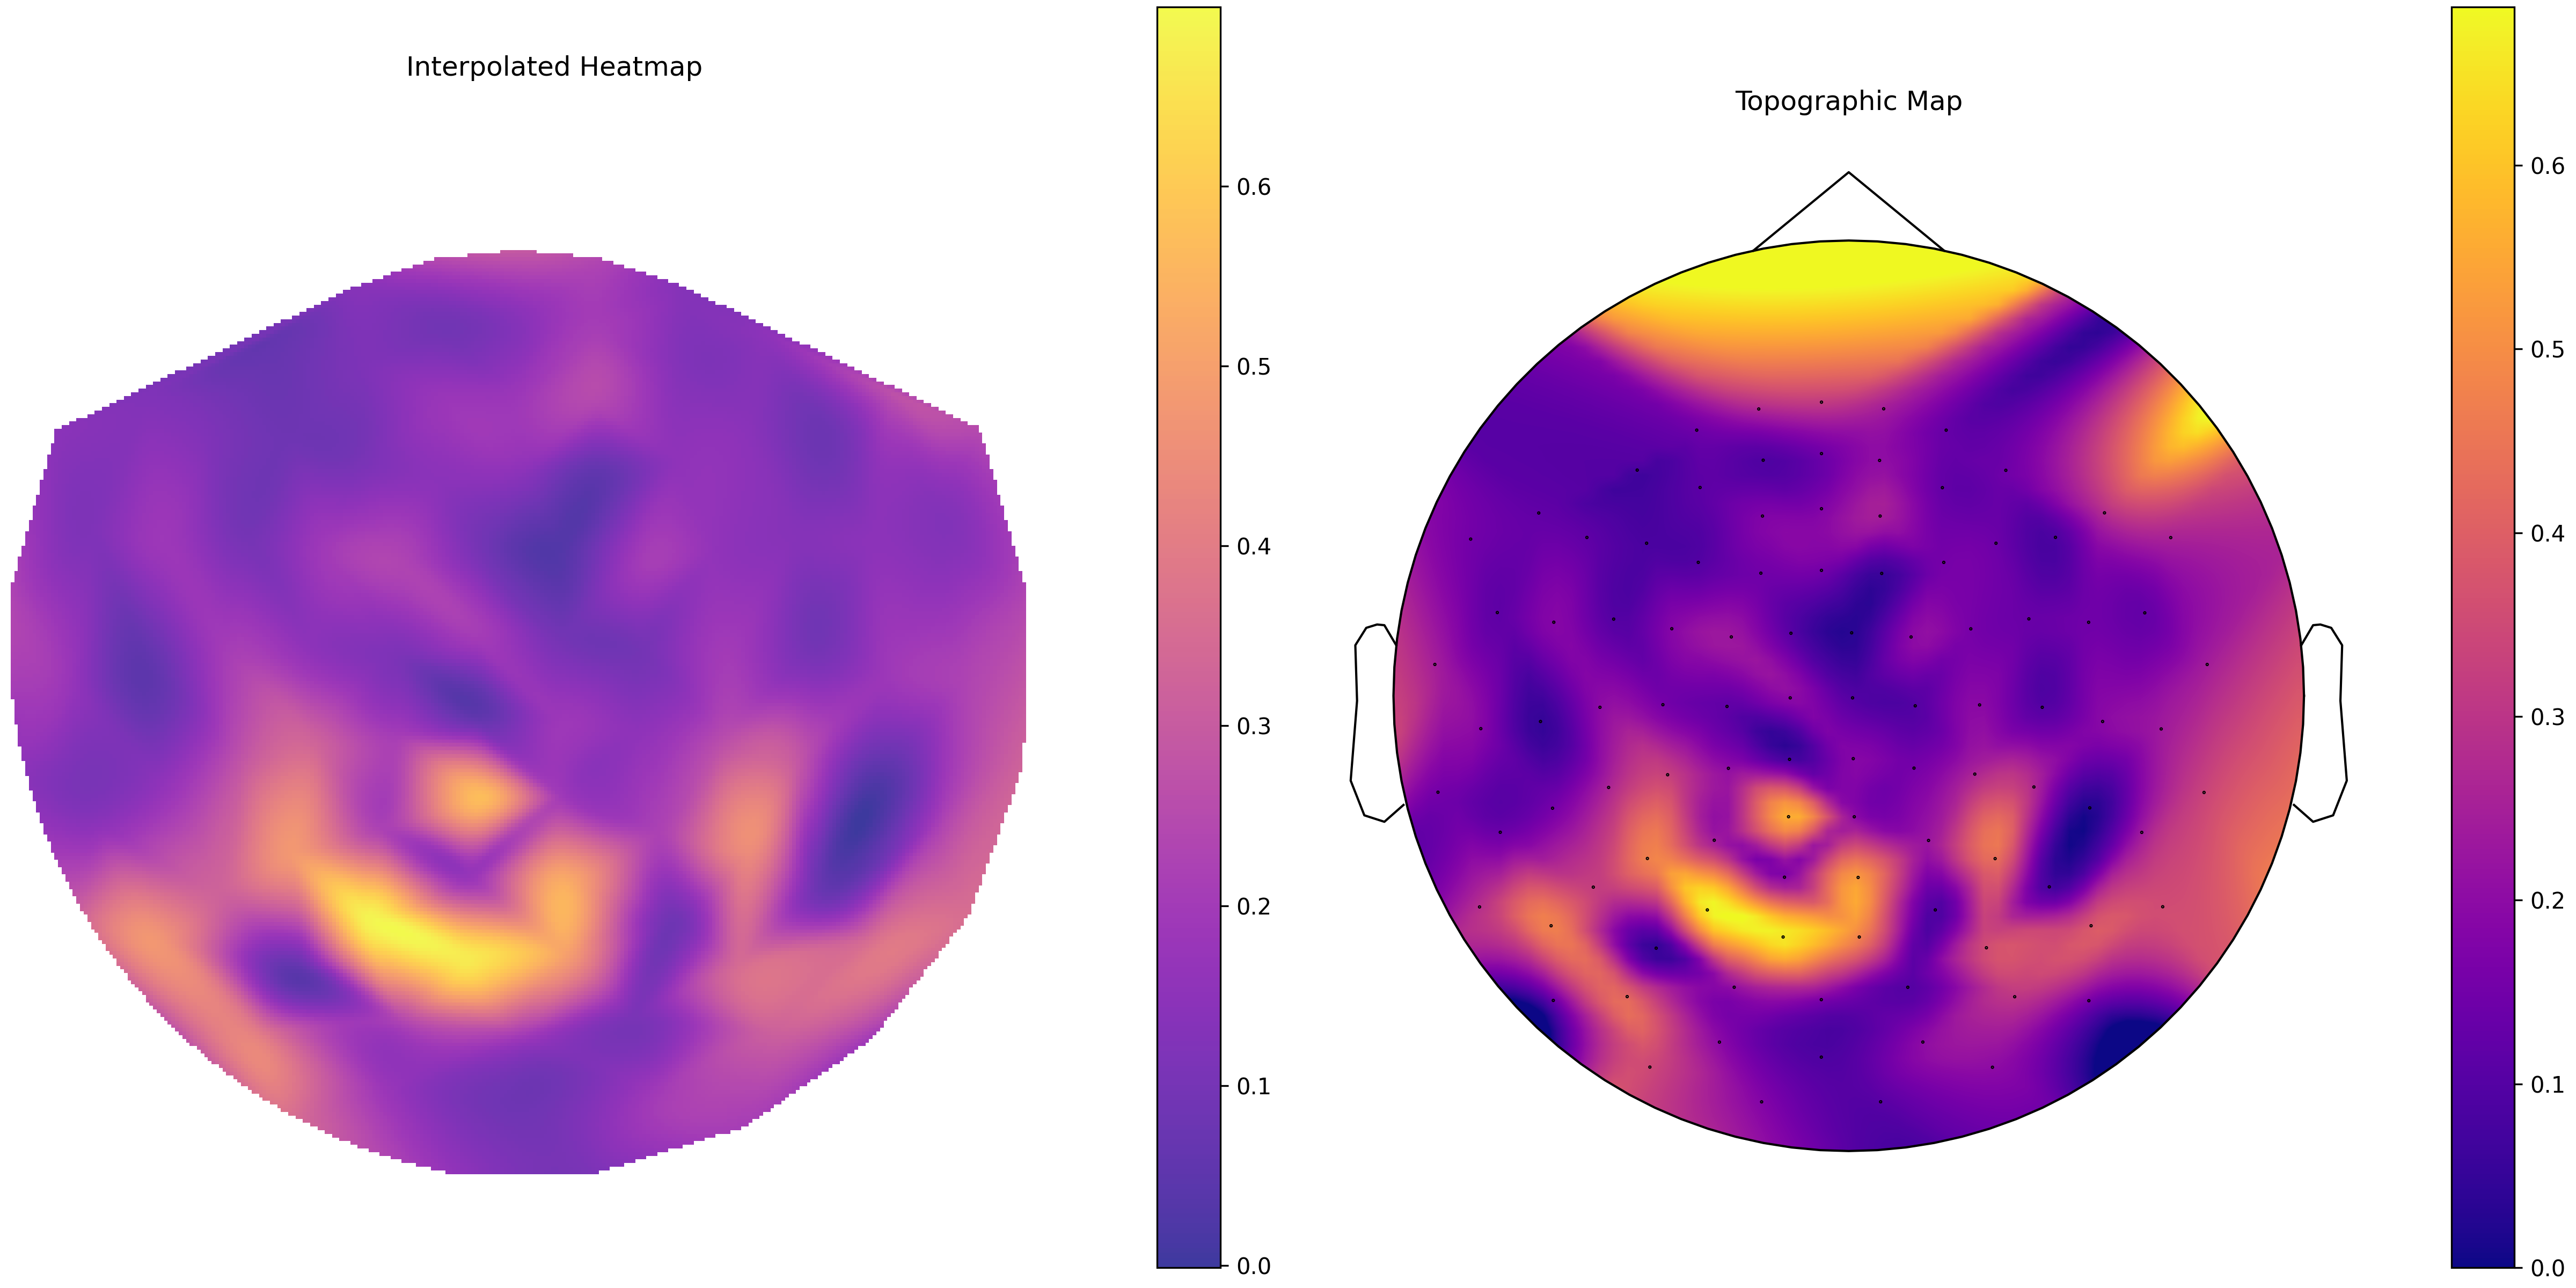
\includegraphics[width=1\textwidth,height=\textheight]{figures/cross-validated-results/linear/imagined-overt-topomap_full.png}
\caption{(a)}\label{fig:imagined-overt-topomap}
\end{figure}

\begin{figure}
\centering
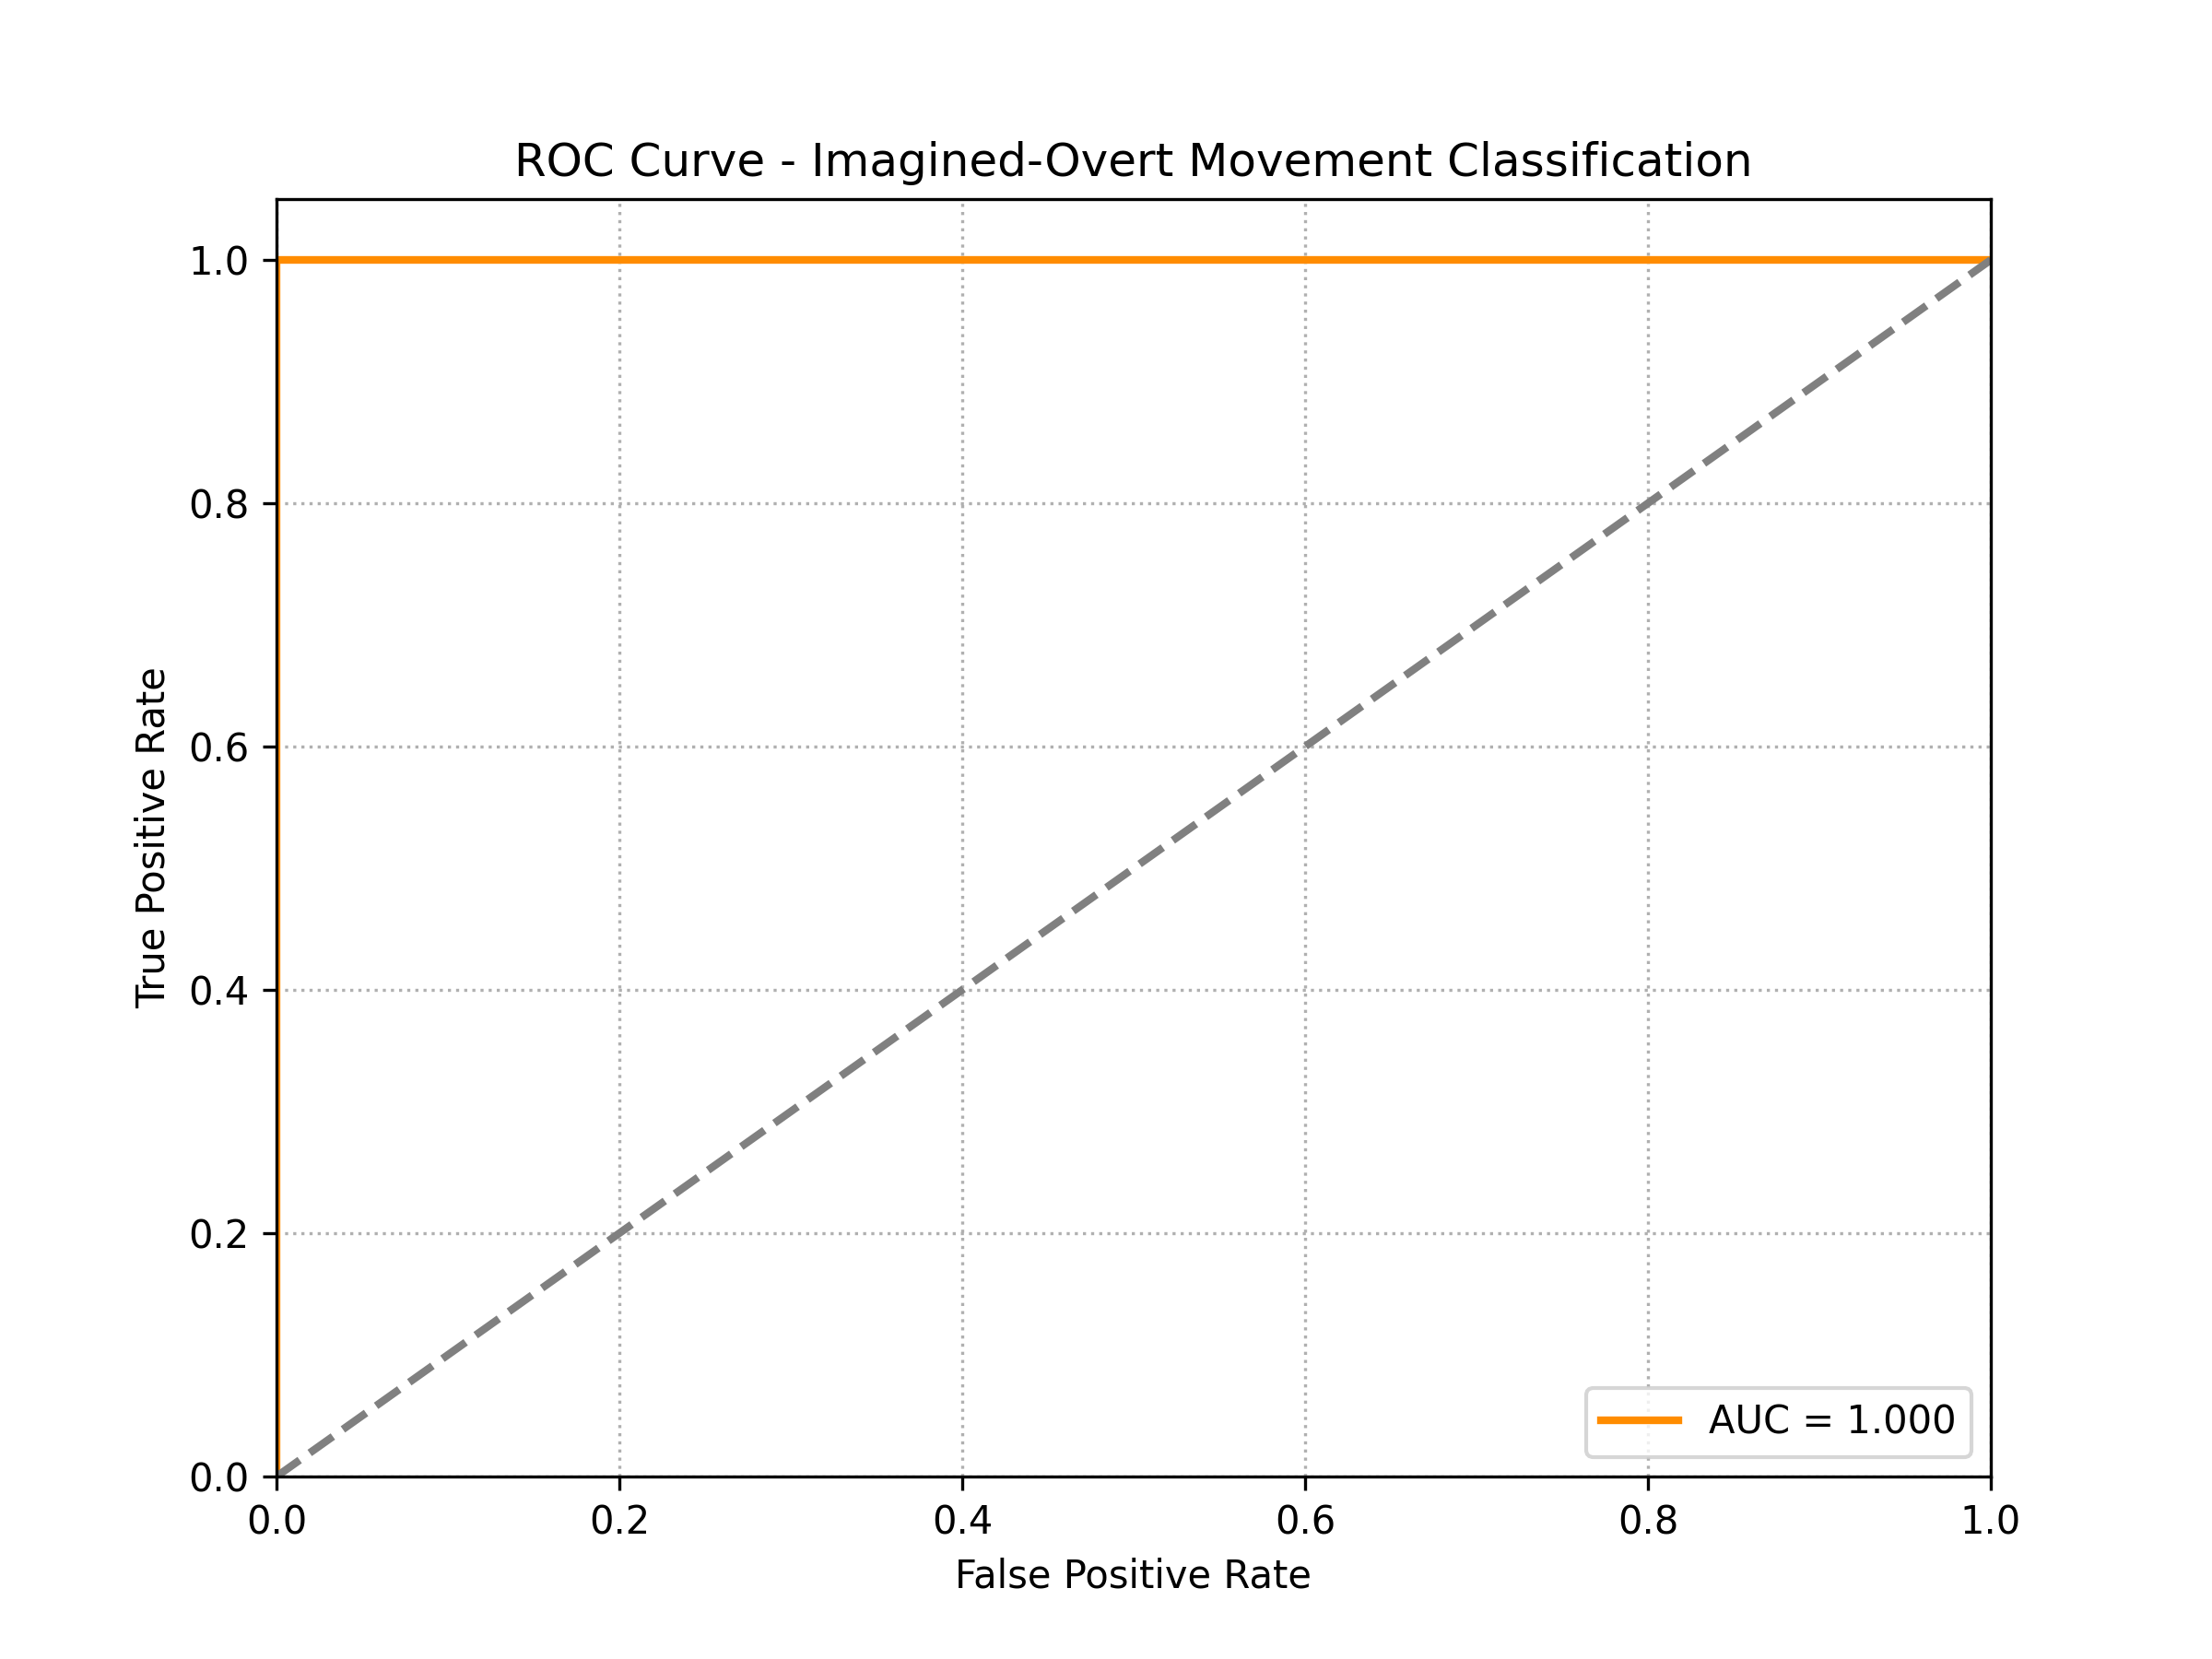
\includegraphics[width=1\textwidth,height=\textheight]{figures/cross-validated-results/linear/imagined-overt-roc-curve.png}
\caption{(b)}\label{fig:imagined-overt-roc}
\end{figure}

\begin{figure}
\centering
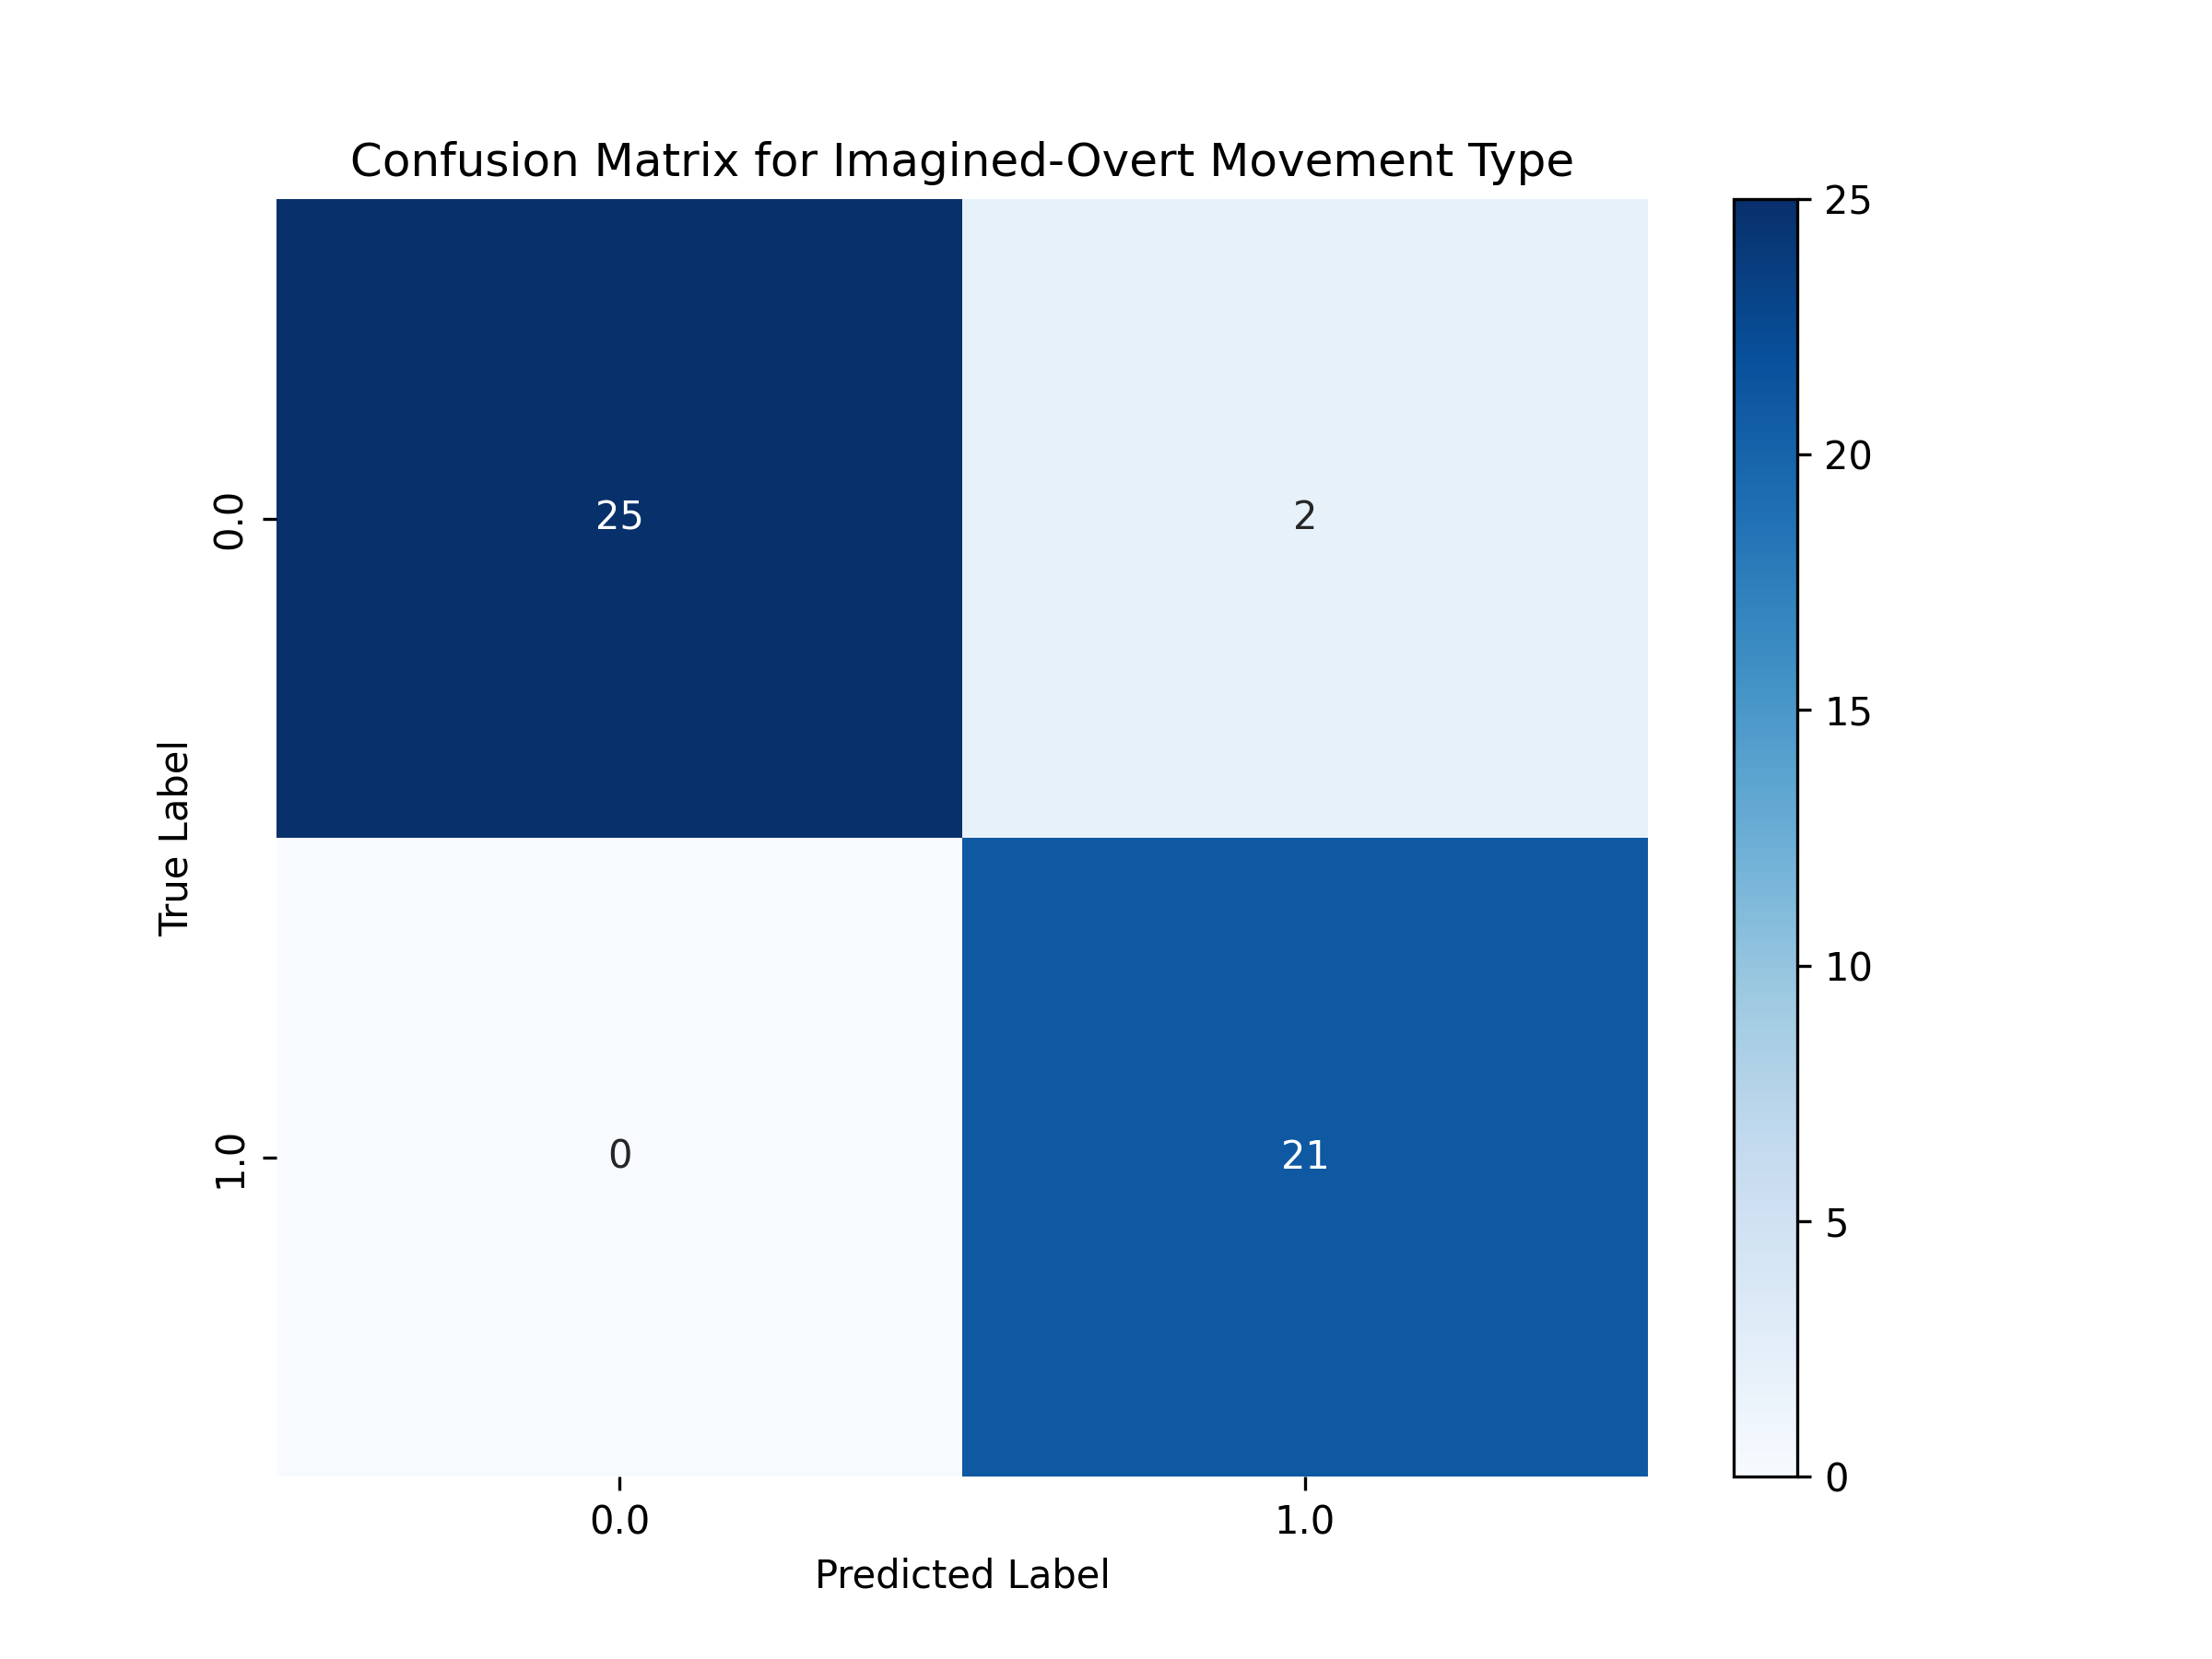
\includegraphics[width=1\textwidth,height=\textheight]{figures/cross-validated-results/linear/imagined-overt-confusion-matrix.png}
\caption{(c)}\label{fig:imagined-overt-confusion-matrix}
\end{figure}

\begin{figure}
\centering
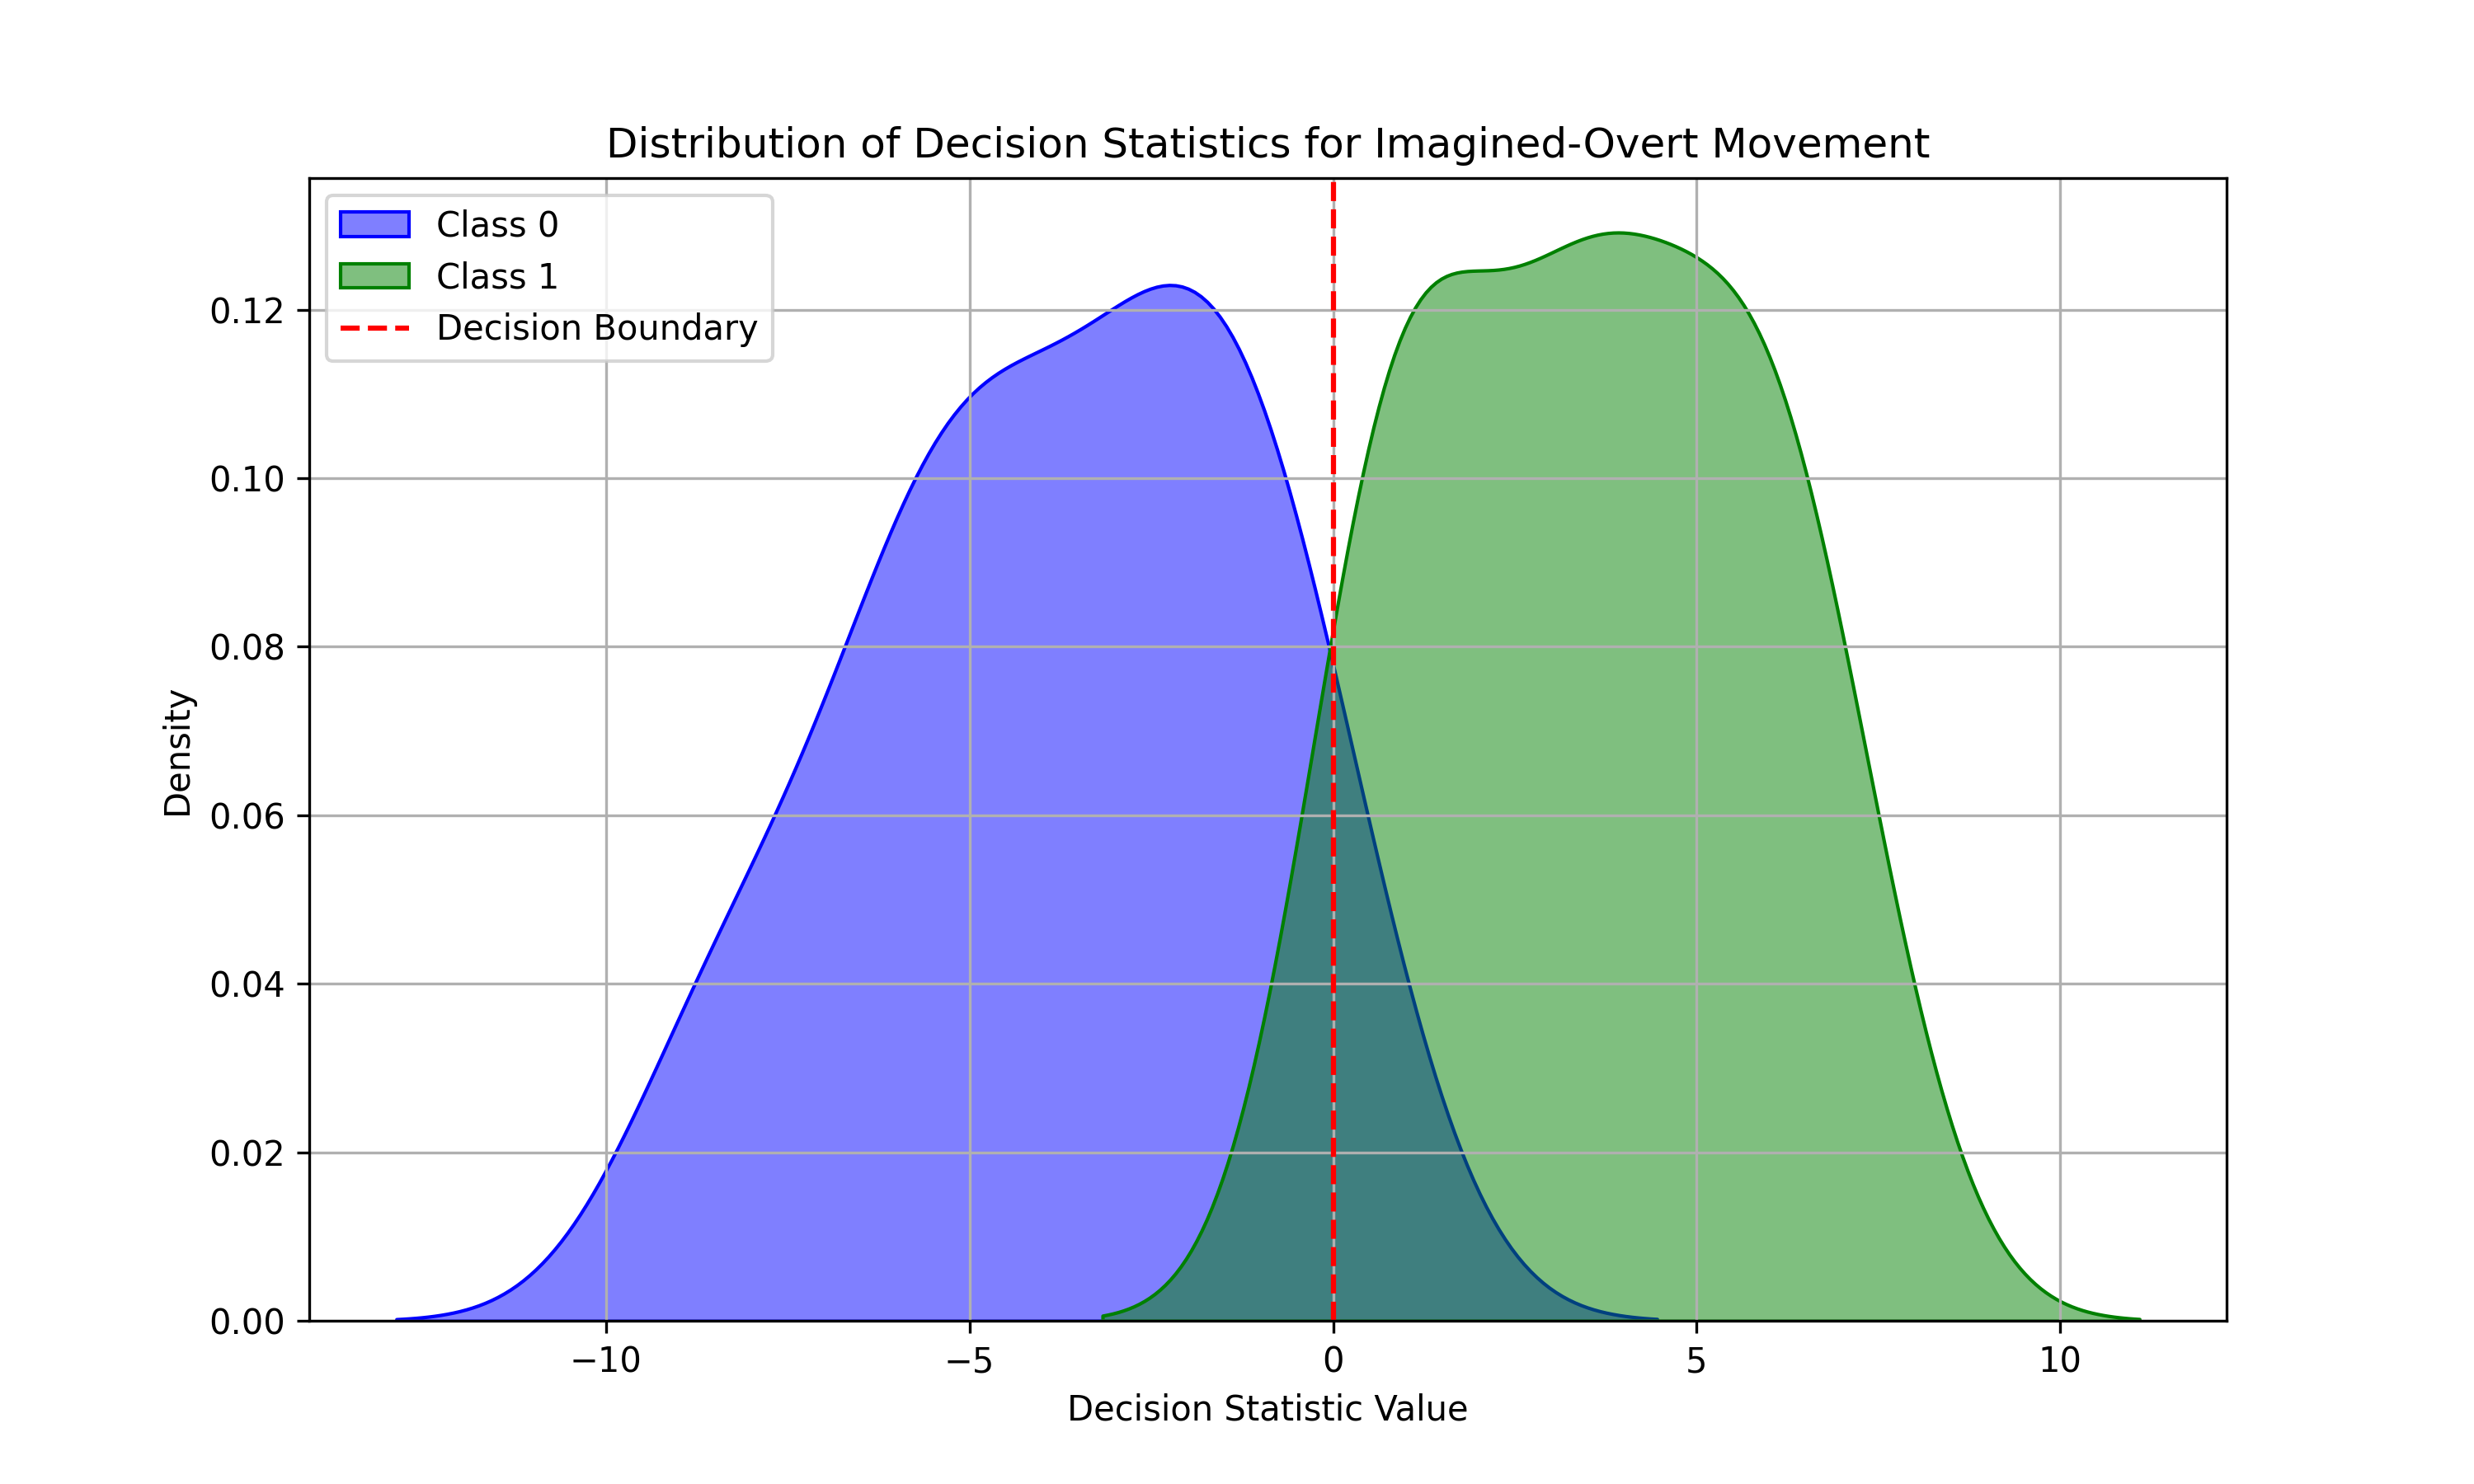
\includegraphics[width=1\textwidth,height=\textheight]{figures/cross-validated-results/linear/imagined-overt-decision-statistic.png}
\caption{(d)}\label{fig:imagined-overt-decision-statistic}
\end{figure}

}

\caption{\label{fig-imagined-overt-results}Imagined to overt movement
classification results: (a) Topographic map showing spatial distribution
of informative electrodes, (b) ROC curve illustrating true positive vs
false positive rates, (c) Confusion matrix indicating classification
performance, and (d) Decision statistic distribution across trials.}

\end{figure}%

\paragraph{Scenario Comparison
Summary}\label{scenario-comparison-summary}

The figure below provides a side-by-side comparison of \textbf{accuracy}
and \textbf{AUC} scores across the four scenarios using a linear SVM. As
expected, performance was highest when training and testing within the
same modality (overt-overt or imagined-imagined). Generalization between
imagined and overt signals proved more difficult but remained
informative.

\begin{longtable}[]{@{}lll@{}}
\toprule\noalign{}
Scenario & Accuracy & AUC \\
\midrule\noalign{}
\endhead
\bottomrule\noalign{}
\endlastfoot
Overt → Overt & 98.9\% & 1.0 \\
Imagined → Imagined & 94.9\% & 0.94 \\
Overt → Imagined & 97.9\% & 0.98 \\
Imagined → Overt & 95.8\% & 0.95 \\
\end{longtable}

These findings emphasize the domain-specific nature of EEG
classification. While classifiers can generalize across signal types to
some extent, model performance is consistently stronger within the same
training and testing modality. This has important implications for BCI
design, particularly when building models intended for use in both
imagined and overt control environments.

\subsection{Kernel SVM Performance and
Interpretability}\label{kernel-svm-performance-and-interpretability}

To explore the effect of different nonlinear transformations on EEG
classification, we trained SVMs using four kernel
types---\textbf{linear}, \textbf{polynomial}, \textbf{RBF}, and
\textbf{sigmoid}---on both imagined and overt movement datasets. All
models used the same regularization search strategy and were evaluated
on a held-out test set using accuracy, ROC-AUC, decision statistics, and
spatial interpretability through topomaps.

Surprisingly, the \textbf{linear kernel consistently outperformed} its
more complex counterparts in both conditions. It not only yielded the
highest test accuracy and AUC but also produced the most stable and
interpretable decision boundaries. The topographic maps generated from
the linear models displayed focused and physiologically plausible
electrode activations, aligning well with expected motor cortex
patterns.

In contrast, while RBF and polynomial kernels offered more flexible
decision surfaces, they did not significantly improve classification and
sometimes introduced noisy or less consistent spatial weight
distributions. The sigmoid kernel performed the weakest overall, showing
high variance and poor generalization in both datasets.

This experiment reinforces an important principle: \textbf{more complex
models do not always outperform simpler ones}, especially when the
signal is already well-structured or when model interpretability is a
priority. In this case, the linear SVM not only proved highly effective
but also enabled detailed spatial insights through clean topographic
visualizations.

\begin{figure}

\centering{

\begin{figure}
\centering
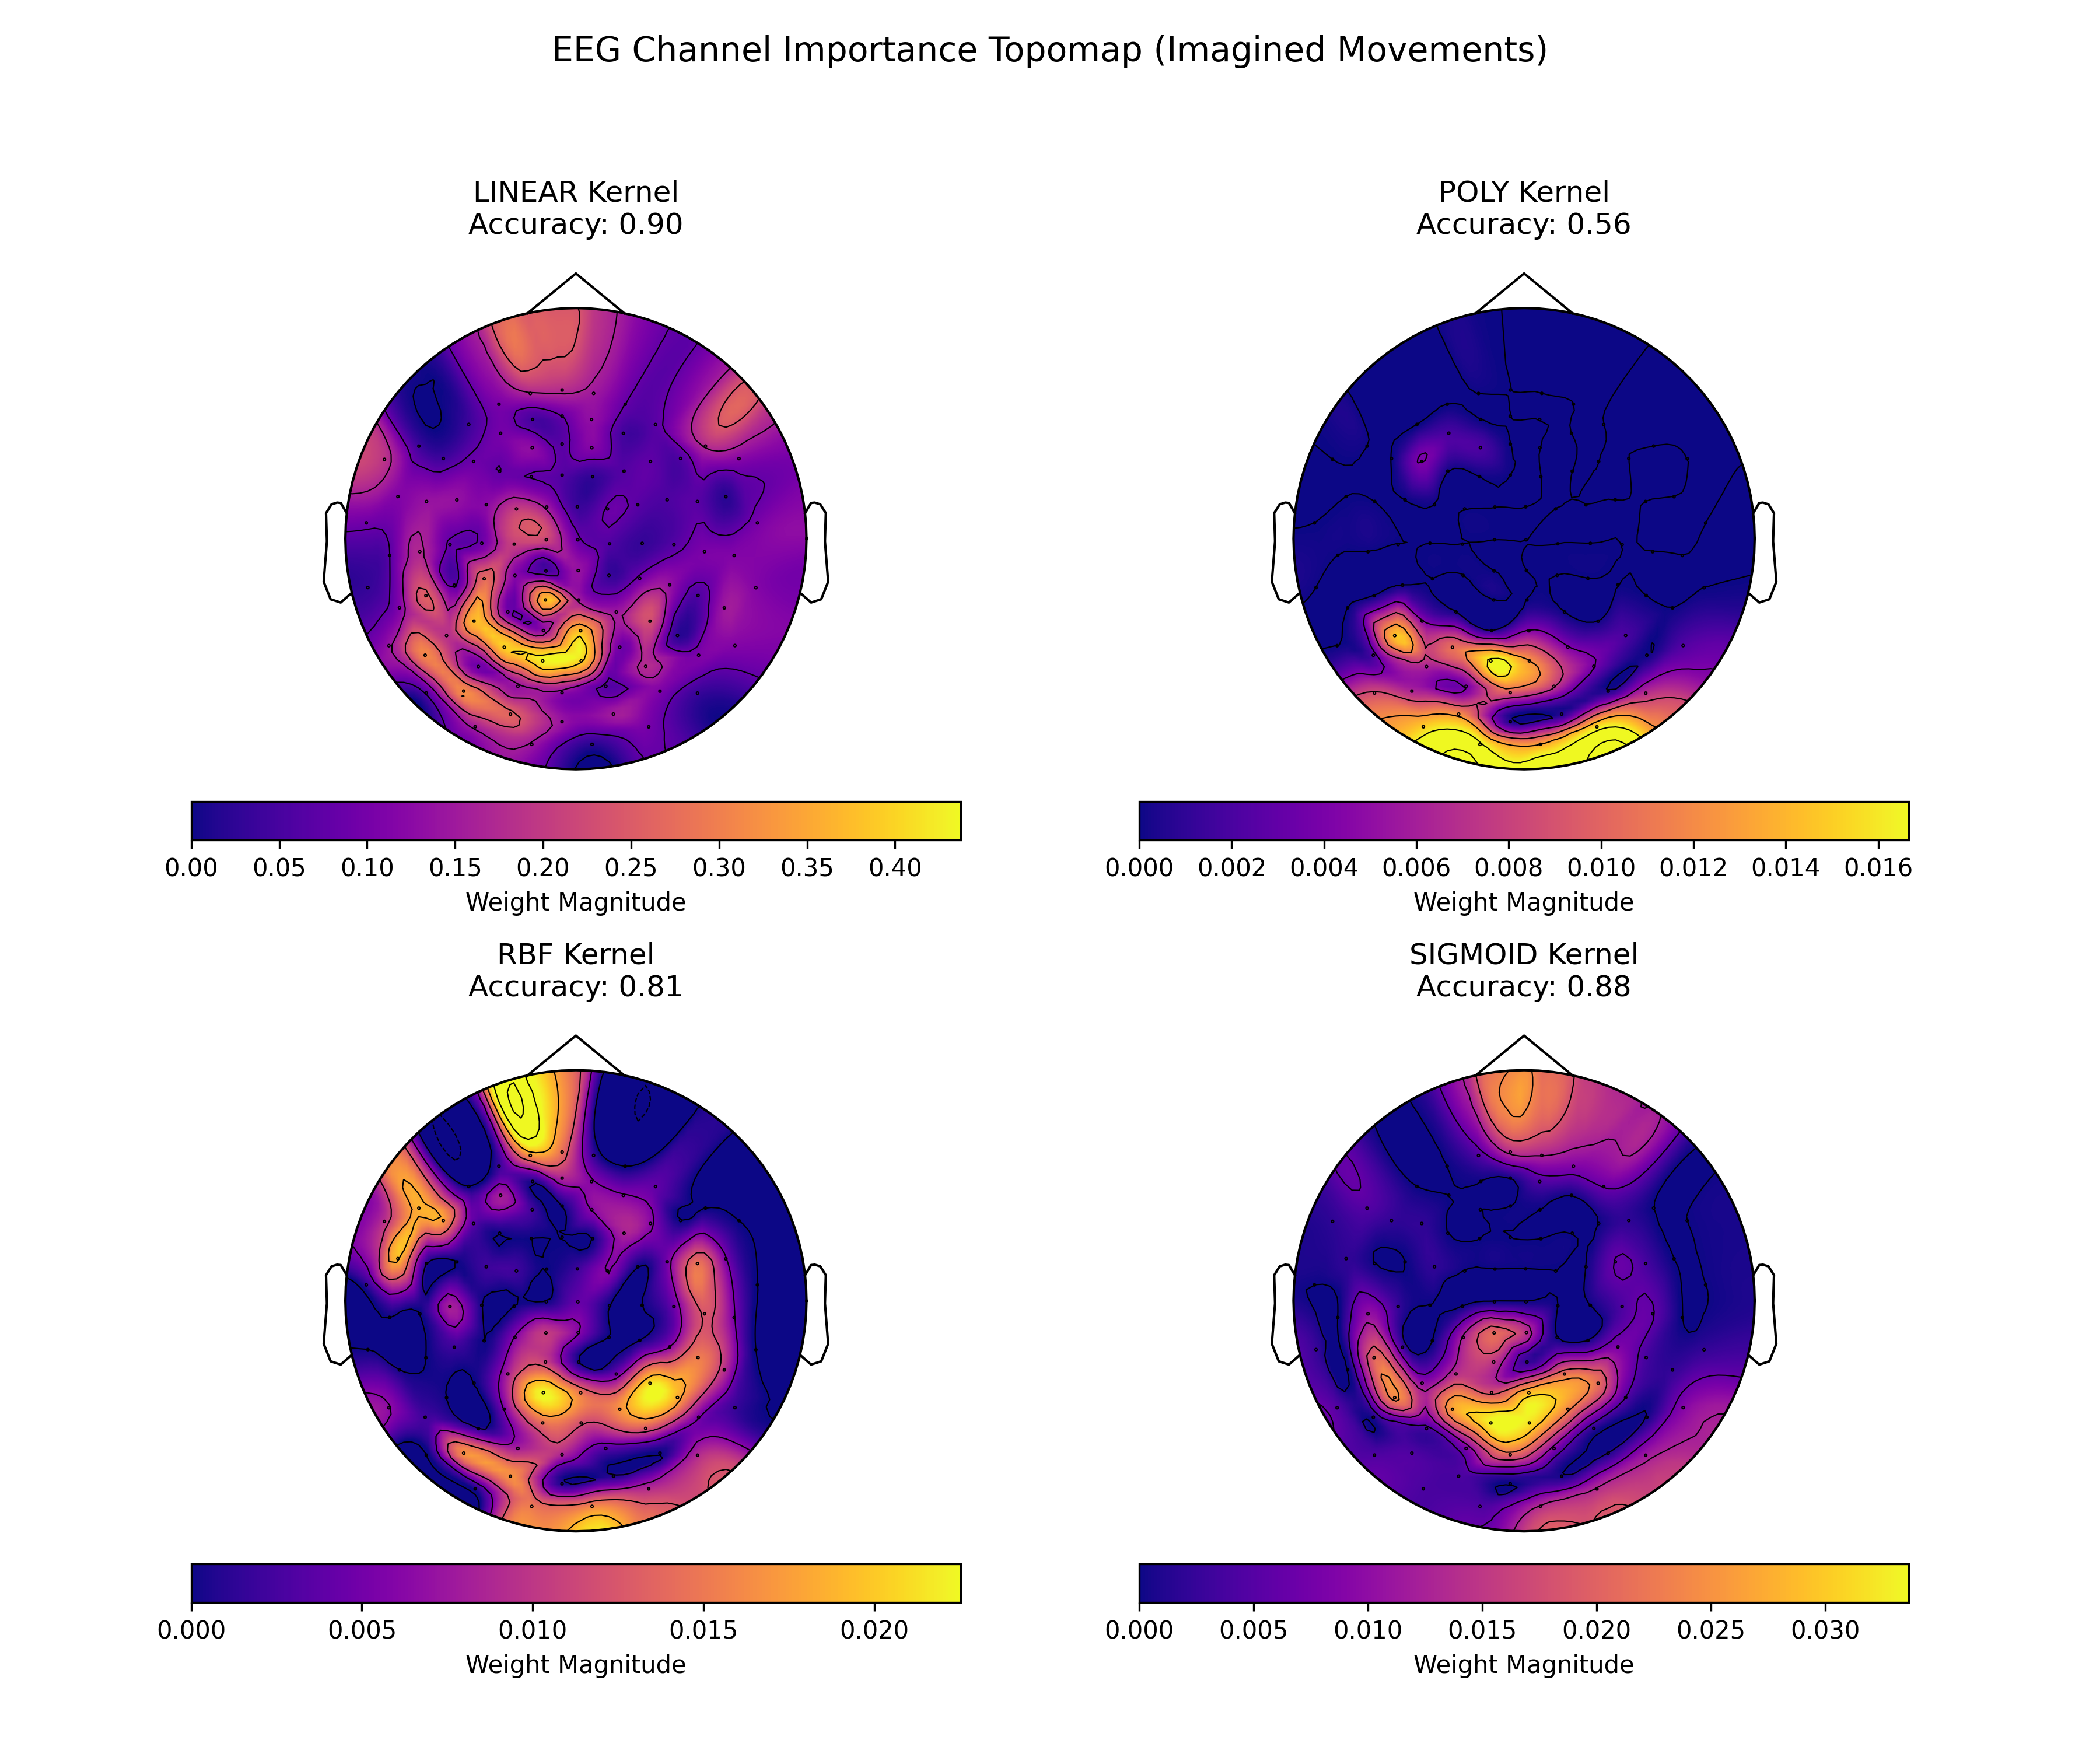
\includegraphics[width=1\textwidth,height=\textheight]{figures/svm_topomaps_all_kernels_imagined.png}
\caption{(a)}\label{fig:topomap-real}
\end{figure}

\begin{figure}
\centering
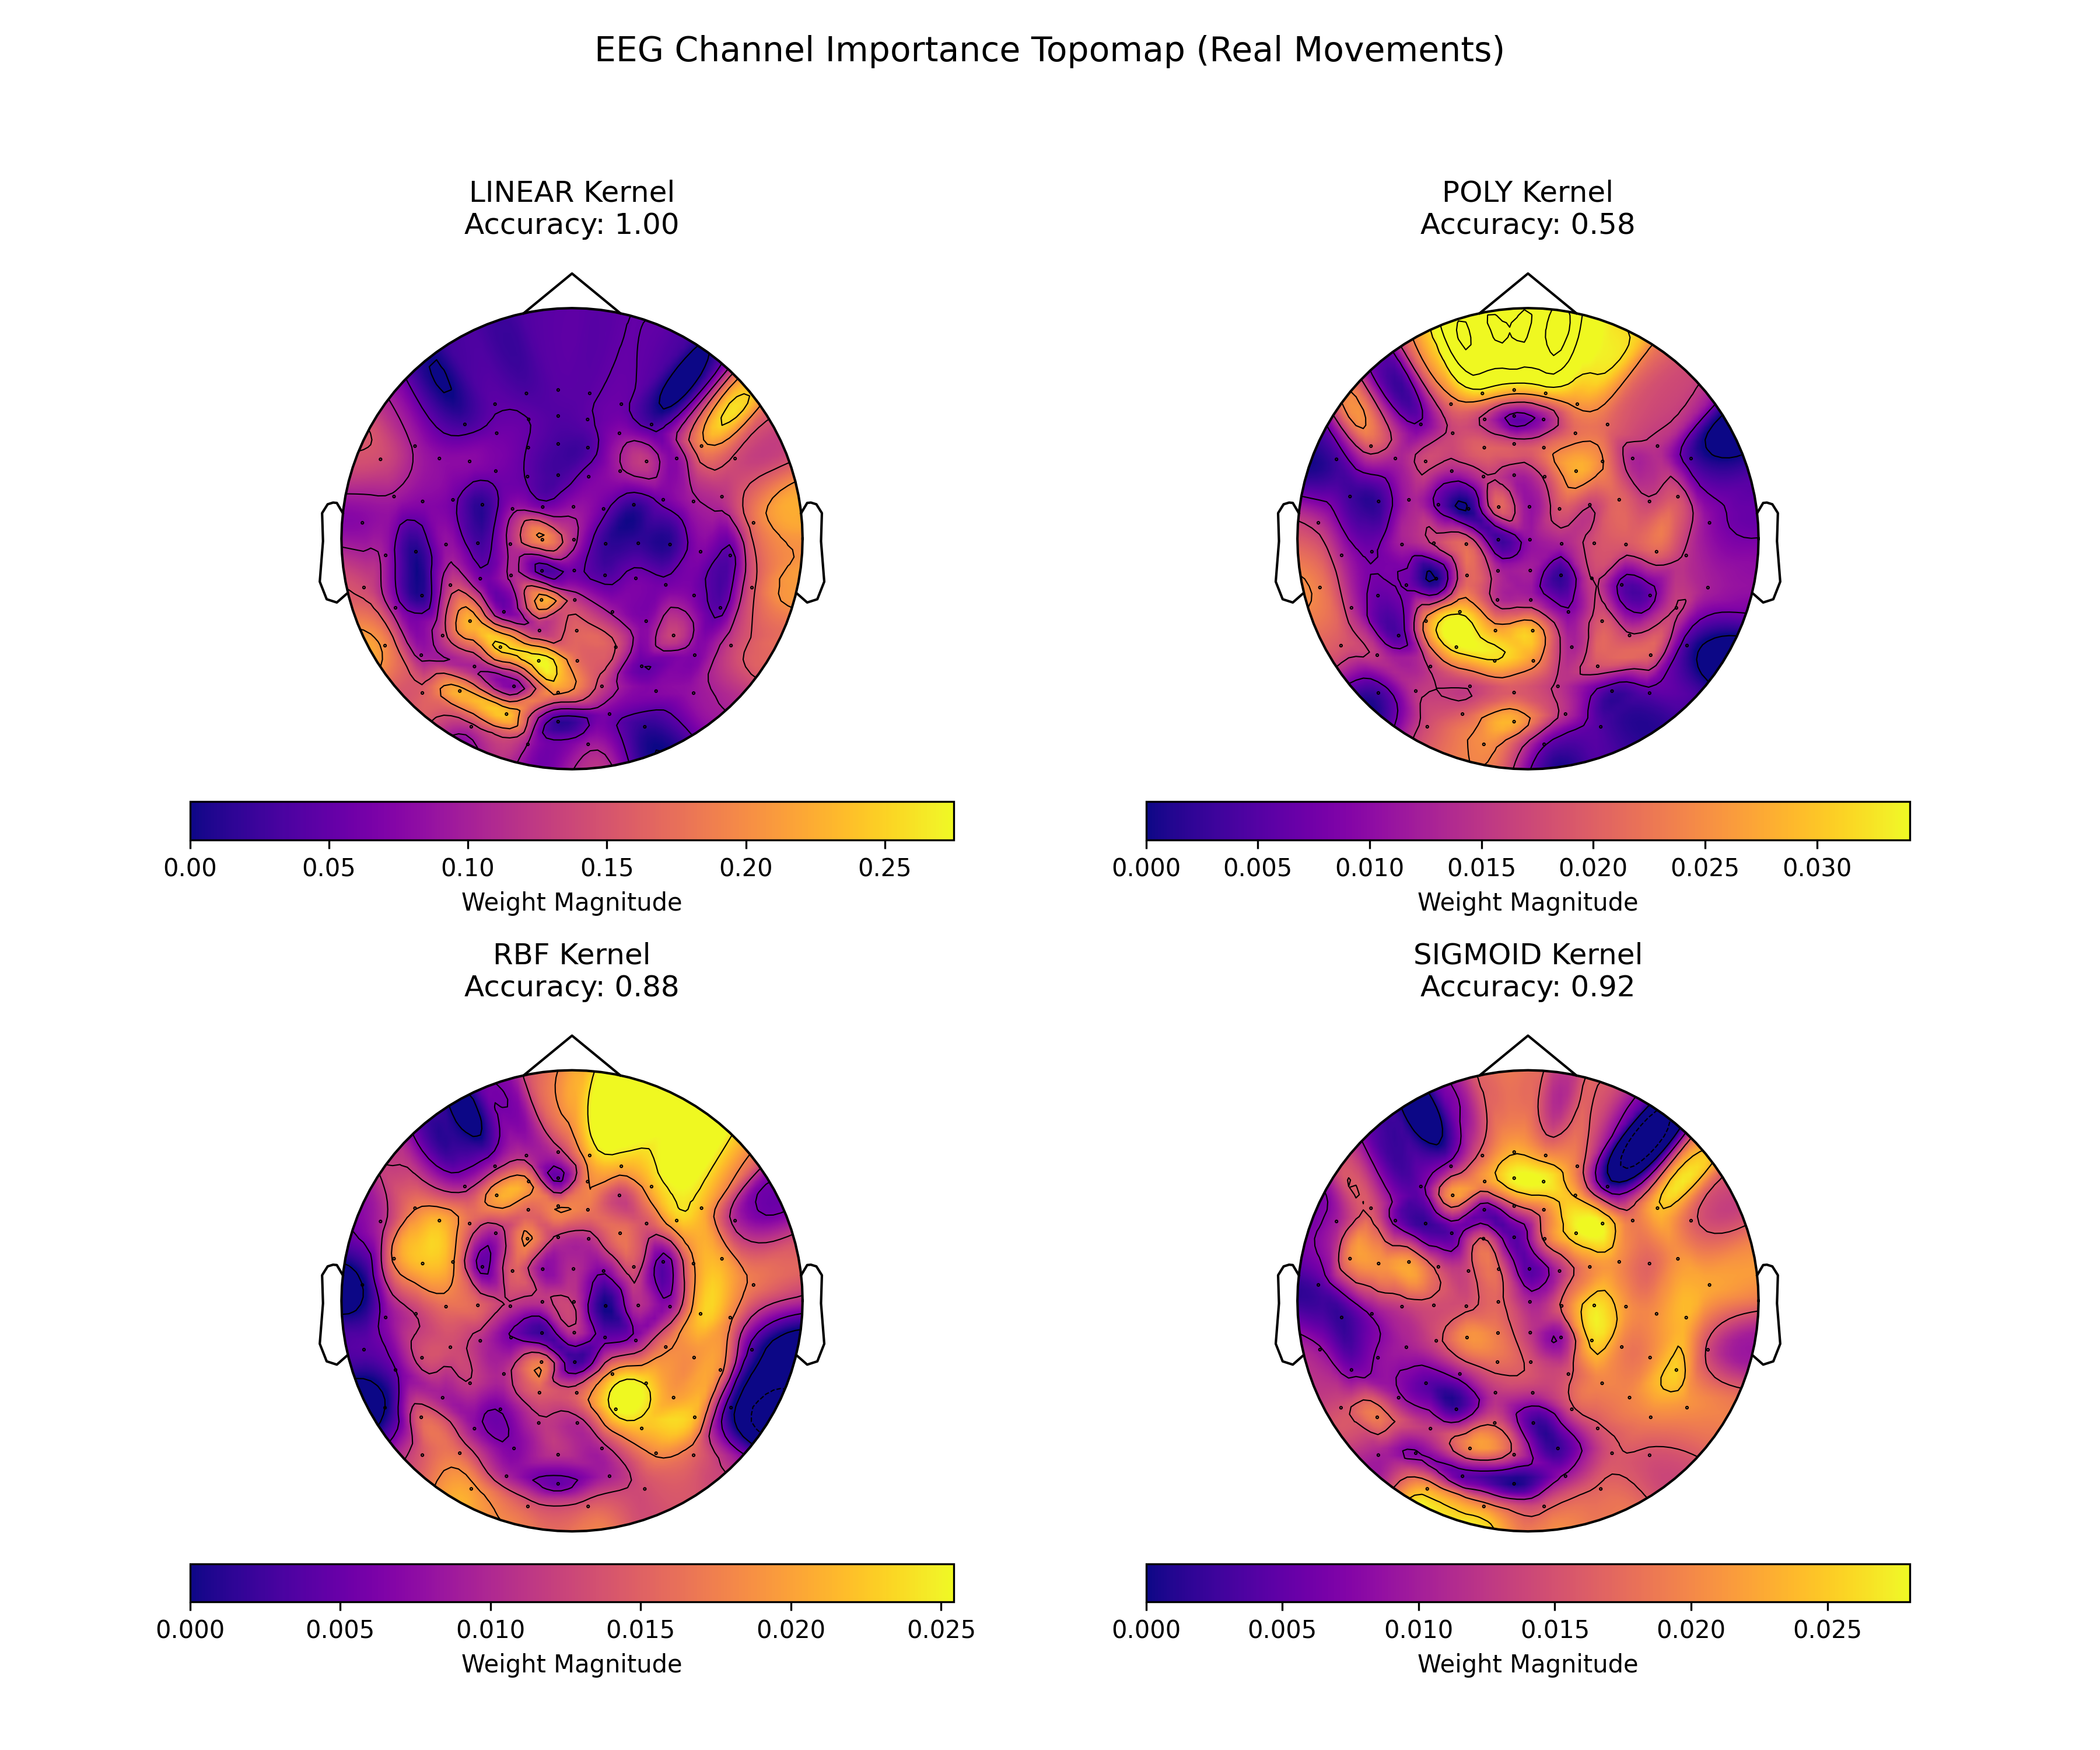
\includegraphics[width=1\textwidth,height=\textheight]{figures/svm_topomaps_all_kernels_real.png}
\caption{(b)}\label{fig:topomap-imagined}
\end{figure}

}

\caption{\label{fig-kernel-comparison}Kernel comparison results: (a)
Topographic maps showing spatial distribution of informative electrodes
for different kernel SVMs on imagined movements, (b) Topographic maps
showing spatial distribution of informative electrodes for different
kernel SVMs on overt movements.}

\end{figure}%

Analyzing the pictures above we can a region is always very relevant for
the decision of the class but it varies depending on the kernel used.
The linear kernel shows a very clear pattern of activation over the
central parietal region, while the RBF kernel shows a more diffuse
pattern of activation. The polynomial kernel shows a similar pattern to
the RBF kernel, but with less intensity. The sigmoid kernel shows a very
diffuse pattern of activation, indicating that it is not able to learn
the underlying patterns in the data.

Interestingly, the linear kernel produced the most interpretable
topographic maps, with clear spatial distributions of informative
electrodes.

\begin{longtable}[]{@{}
  >{\raggedright\arraybackslash}p{(\columnwidth - 6\tabcolsep) * \real{0.1558}}
  >{\raggedright\arraybackslash}p{(\columnwidth - 6\tabcolsep) * \real{0.2468}}
  >{\raggedright\arraybackslash}p{(\columnwidth - 6\tabcolsep) * \real{0.1948}}
  >{\raggedright\arraybackslash}p{(\columnwidth - 6\tabcolsep) * \real{0.4026}}@{}}
\toprule\noalign{}
\begin{minipage}[b]{\linewidth}\raggedright
Kernel
\end{minipage} & \begin{minipage}[b]{\linewidth}\raggedright
Imagined Accuracy
\end{minipage} & \begin{minipage}[b]{\linewidth}\raggedright
Real Accuracy
\end{minipage} & \begin{minipage}[b]{\linewidth}\raggedright
Notes
\end{minipage} \\
\midrule\noalign{}
\endhead
\bottomrule\noalign{}
\endlastfoot
Linear & 0.96 & 0.96 & Best performer, interpretable \\
RBF & 0.79 & 0.85 & Flexible, but no performance gain \\
Polynomial & 0.62 & 0.73 & Moderate performance, overfit-prone \\
Sigmoid & 0.79 & 0.90 & Weak performance, high variance \\
\end{longtable}

\section{Conclusion}\label{conclusion}

This project explored the use of Support Vector Machines (SVMs) for
classifying EEG data related to motor activity, both overt and imagined.
The project was conducted in alignment with the ECE 580 mini-project
requirements and involved rigorous experimentation across multiple
dimensions of model complexity, validation, and modality-specific
generalization.

One of the central contributions of this work was the implementation of
a \textbf{two-level nested cross-validation} pipeline. This method
proved essential for selecting regularization parameters in a
statistically robust manner, ensuring that hyperparameter tuning was
fully decoupled from final model evaluation. In high-dimensional,
low-sample-size contexts like EEG, this methodological rigor is critical
to producing generalizable and reproducible results.

Another key takeaway was the \textbf{surprising strength of the linear
SVM}, especially in comparison to more complex kernel-based models.
Despite testing polynomial, RBF, and sigmoid kernels, the linear SVM
consistently delivered the best overall performance in both imagined and
overt movement classification tasks. It also yielded the clearest
spatial patterns in topographic maps, enabling interpretable
visualizations of channel relevance. This finding underscores a vital
lesson in applied machine learning: \textbf{simplicity can outperform
complexity when the data is well-structured and the model is
appropriately regularized}.

The results showed:

\begin{itemize}
\tightlist
\item
  \textbf{High classification accuracy and AUC in within-modality
  scenarios}, particularly Overt → Overt.
\item
  \textbf{Non-trivial classification performance even in Imagined →
  Imagined}, despite the known challenges with such data.
\item
  \textbf{Limited but meaningful generalization across modalities}
  (e.g., Overt → Imagined), suggesting shared spatial features that
  models can exploit even under signal mismatch.
\item
  \textbf{L2 regularization generally outperforming L1}, except in some
  transfer cases where sparsity favored L1.
\end{itemize}

From a practical standpoint, the ability to decode motor intent from EEG
using interpretable and computationally efficient models like linear
SVMs makes this approach highly attractive for real-time Brain-Computer
Interface (BCI) systems. The clean separation achieved with simple
models reduces both training complexity and latency, which are vital
considerations in interactive neurotechnologies.

This project was made possible through collaborative support:

\begin{itemize}
\tightlist
\item
  The \textbf{ECE580 course instruction team}, for providing
  well-defined datasets and a detailed project scaffold.
\item
  \textbf{Class peers and the Colab@Duke community}, who offered
  valuable discussions on model tuning and visualization strategies.
\item
  The open-source contributions of MNE-Python, scikit-learn, and UMAP
  libraries, which enabled the advanced spatial and decision-surface
  visualizations that enhanced the interpretability of this work.
\end{itemize}

\subsubsection{Next Steps and Future
Directions}\label{next-steps-and-future-directions}

One of the most immediate next steps involves expanding the evaluation
to larger and more diverse datasets, including different subjects or
session conditions. The current results were obtained on single-session
data, and testing generalization across individuals would provide
stronger evidence for real-world applicability. Additionally, although
this study focused on static trial-level inputs, future efforts could
explore more dynamic classification pipelines that operate continuously
on streaming EEG data---moving toward real-time decoding scenarios.

There is also significant potential in deploying the trained models
within real-time Brain-Computer Interface (BCI) systems. Given the low
computational overhead of linear SVMs, these models are ideally suited
for real-time classification engines that could be integrated with
digital interfaces or assistive technologies. For example, the
classifier could be used to trigger directional input commands based on
imagined movements, enabling control of cursors, robotic arms, or
external software environments.

Moreover, the simplicity of the linear SVM model makes it a strong
candidate for implementation on embedded systems such as Raspberry Pi or
microcontroller units, allowing classification to occur on-device
without requiring high-power computing resources. This would open doors
for the development of portable, low-cost, and scalable EEG-based
systems for use in accessibility or rehabilitation contexts.

\subsubsection{Final Remarks}\label{final-remarks}

While many machine learning projects assume that increasing model
complexity guarantees better performance, this work serves as a
counterexample rooted in neuroscience. The structure of EEG
signals---and the spatially organized nature of motor-related brain
activity---lends itself well to \textbf{linear classification models},
provided the preprocessing and validation are carefully performed.

This study not only achieved strong technical results but also
highlighted the importance of methodical design, model interpretability,
and simplicity---principles that will continue to guide future work in
brain-computer interface research and beyond.

\section{References}\label{references}

\subsection{Colaboration}\label{colaboration}

\begin{itemize}
\tightlist
\item
  Peter Banyas - Discussed and provided feedback on the project related
  to decision statistics and topographic maps.
\item
  Pedro Melo - Provided valuable insights on the use of UMAP for
  dimensionality reduction and visualization.
\end{itemize}

\subsection{Packages used}\label{packages-used}

\begin{itemize}
\tightlist
\item
  Scikit-learn: Used for implementing and evaluating SVM classifiers,
  performing grid search, and calculating performance metrics like
  accuracy and ROC-AUC {[}7{]}.
\item
  NumPy: Used for numerical operations and handling arrays efficiently
  {[}8{]}.
\item
  Pandas: Used for data manipulation and analysis, particularly for
  loading and preprocessing the EEG datasets {[}9{]}.
\item
  Matplotlib: Used for creating visualizations, including topographic
  maps and ROC curves {[}10{]}.
\item
  Seaborn: Used for enhancing the aesthetics of visualizations,
  particularly confusion matrices {[}11{]}.
\item
  MNE: Used for EEG data processing, including filtering, epoching, and
  topographic map generation {[}12{]}.
\item
  UMAP: Used for dimensionality reduction and visualization of
  high-dimensional EEG data {[}13{]}.
\end{itemize}

\phantomsection\label{refs}
\begin{CSLReferences}{0}{0}
\bibitem[\citeproctext]{ref-5953178}
\CSLLeftMargin{{[}1{]} }%
\CSLRightInline{A. R. Mathew, A. Al Hajj, and A. Al Abri,
{``Human-computer interaction (HCI): An overview,''} in \emph{2011 IEEE
international conference on computer science and automation
engineering}, 2011, pp. 99--100. doi:
\href{https://doi.org/10.1109/CSAE.2011.5953178}{10.1109/CSAE.2011.5953178}.}

\bibitem[\citeproctext]{ref-Costantini2009}
\CSLLeftMargin{{[}2{]} }%
\CSLRightInline{G. Costantini \emph{et al.}, {``{SVM Classification of
EEG Signals for Brain Computer Interface},''} in \emph{{Neural Nets
WIRN09}}, IOS Press, 2009, pp. 229--233. doi:
\href{https://doi.org/10.3233/978-1-60750-072-8-229}{10.3233/978-1-60750-072-8-229}.}

\bibitem[\citeproctext]{ref-8606765}
\CSLLeftMargin{{[}3{]} }%
\CSLRightInline{Y.-T. Wu, T. H. Huang, C. Yi Lin, S. J. Tsai, and P.-S.
Wang, {``Classification of EEG motor imagery using support vector
machine and convolutional neural network,''} in \emph{2018 international
automatic control conference (CACS)}, 2018, pp. 1--4. doi:
\href{https://doi.org/10.1109/CACS.2018.8606765}{10.1109/CACS.2018.8606765}.}

\bibitem[\citeproctext]{ref-9131312}
\CSLLeftMargin{{[}4{]} }%
\CSLRightInline{T. Dai and Y. Dong, {``Introduction of SVM related
theory and its application research,''} in \emph{2020 3rd international
conference on advanced electronic materials, computers and software
engineering (AEMCSE)}, 2020, pp. 230--233. doi:
\href{https://doi.org/10.1109/AEMCSE50948.2020.00056}{10.1109/AEMCSE50948.2020.00056}.}

\bibitem[\citeproctext]{ref-MELKUMOVA2017746}
\CSLLeftMargin{{[}5{]} }%
\CSLRightInline{L. E. Melkumova and S. Ya. Shatskikh, {``Comparing ridge
and LASSO estimators for data analysis,''} \emph{Procedia Engineering},
vol. 201, pp. 746--755, 2017, doi:
\url{https://doi.org/10.1016/j.proeng.2017.09.615}.}

\bibitem[\citeproctext]{ref-BibEntry2025Apr}
\CSLLeftMargin{{[}6{]} }%
\CSLRightInline{M. W. S., {``{neuromappr},''} \emph{GitHub}. Apr. 2025.
Accessed: Apr. 27, 2025. {[}Online{]}. Available:
\url{https://github.com/Wanghley/neuromappr}}

\bibitem[\citeproctext]{ref-scikit-learn}
\CSLLeftMargin{{[}7{]} }%
\CSLRightInline{F. Pedregosa \emph{et al.}, \emph{Scikit-learn: Machine
learning in {P}ython}, vol. 12. 2011, pp. 2825--2830.}

\bibitem[\citeproctext]{ref-numpy}
\CSLLeftMargin{{[}8{]} }%
\CSLRightInline{C. R. Harris \emph{et al.}, \emph{Array programming with
NumPy}, vol. 585. Nature Publishing Group, 2020, pp. 357--362.}

\bibitem[\citeproctext]{ref-pandas}
\CSLLeftMargin{{[}9{]} }%
\CSLRightInline{W. McKinney \emph{et al.}, \emph{Pandas: A foundational
python library for data analysis and statistics}. 2011.}

\bibitem[\citeproctext]{ref-matplotlib}
\CSLLeftMargin{{[}10{]} }%
\CSLRightInline{J. D. Hunter, \emph{Matplotlib: A 2D graphics
environment}, vol. 9. IEEE Computer Society, 2007, pp. 90--95.}

\bibitem[\citeproctext]{ref-seaborn}
\CSLLeftMargin{{[}11{]} }%
\CSLRightInline{M. Waskom, \emph{Seaborn: Statistical data
visualization}, vol. 6. 2021, p. 3021.}

\bibitem[\citeproctext]{ref-mne}
\CSLLeftMargin{{[}12{]} }%
\CSLRightInline{A. Gramfort \emph{et al.}, \emph{MNE software for
processing MEG and EEG data}, vol. 86. 2014, pp. 446--460.}

\bibitem[\citeproctext]{ref-umap}
\CSLLeftMargin{{[}13{]} }%
\CSLRightInline{L. McInnes, J. Healy, and J. Melville, \emph{UMAP:
Uniform manifold approximation and projection for dimension reduction}.
2018. Available: \url{https://arxiv.org/abs/1802.03426}}

\end{CSLReferences}




\end{document}
